\documentclass[10pt,a4paper,notitlepage,twocolumn,oneside]{article}

\usepackage[utf8]{inputenc}
\usepackage[a4paper,left=0.15in,right=0.15in,top=0.6in,bottom=0.6in]{geometry}
\usepackage{amsmath,amssymb,amsfonts}
\usepackage{hyperref}
\usepackage{graphicx}
\usepackage{endnotes}
\usepackage{fancyhdr}
\usepackage{titlesec}
\usepackage{setspace}
\usepackage{xcolor}
\usepackage{wrapfig}
\usepackage[font=footnotesize]{subcaption}
\usepackage{longtable,ltcaption}
\usepackage{xtab}
\usepackage{multirow}
\usepackage{array}
\usepackage{enumitem}
%\usepackage[american]{babel}
\usepackage{csquotes}
\usepackage{pdflscape}
\usepackage{comment}
\usepackage[backend=biber,
            style=apa,
            %style=numeric-comp,
            citestyle=authoryear-comp,
            %citestyle=numeric-comp,
            sorting=nyt,
            %sorting=none,
            %maxcitenames=2,
            %mincitenames=1
            ]{biblatex}

%% MACROS
\renewcommand{\footnoterule}{%
  \kern -3pt
  \hrule width \columnwidth height 0.1pt
  \kern 4.5pt
}
\newcommand{\orcid}[1]{\href{https://orcid.org/#1}{
\includegraphics[width=1em]{orcid.pdf}}}
\newcommand{\scholar}[1]{\href{https://scholar.google.pt/citations?user=#1}{
\includegraphics[width=1em]{scholar.pdf}}}

%% GENERAL DEFINITIONS
\DeclareUnicodeCharacter{0301}{\'{e}}
\urlstyle{same}
\DeclareCiteCommand{\citetitle}
  {\boolfalse{citetracker}%
   \boolfalse{pagetracker}%
   \usebibmacro{prenote}}
  {\ifciteindex
     {\indexfield{indextitle}}
     {}%
   \printtext[bibhyperref]{\printfield[citetitle]{labeltitle}}}
  {\multicitedelim}
  {\usebibmacro{postnote}}
\newcolumntype{P}[1]{>{\centering\arraybackslash}p{#1}}
\renewcommand{\arraystretch}{1.25}
\setlength{\tabcolsep}{3pt}

%% HEADINGS
\pagestyle{myheadings}
%\fancyhf{}
\markboth{Ricardo B. Sousa \textit{et al.}}{A Systematic Literature Review on Long-Term Localization and Mapping for Mobile Robots}

%% BIBLATEX
\addbibresource{references.bib}



%%%%%%%%%%%%%%%%%%%% ARTICLE INFORMATION

\title{A Systematic Literature Review on Long-Term Localization and Mapping\\for Mobile Robots%
\thanks{%
This work is financed by National Funds through the Portuguese funding agency, FCT -- Fundação para a Ciência e a Tecnologia, within scholarship 2021.04591.BD.

\vspace{1em}
\noindent Ricardo B. Sousa\textsuperscript{1, 2}

\noindent \href{mailto:up201503004@edu.fe.up.pt}{up201503004@edu.fe.up.pt}

\vspace{0.5em}
\noindent H\'{e}ber M. Sobreira\textsuperscript{2}

\noindent \href{mailto:heber.m.sobreira@inesctec.pt}{heber.m.sobreira@inesctec.pt}

\vspace{0.5em}
\noindent Ant\'{o}nio Paulo Moreira\textsuperscript{1, 2}

\noindent \href{mailto:amoreira@fe.up.pt}{amoreira@fe.up.pt}

\vspace{1em}
\noindent \textsuperscript{1} Faculty of Engineering of the University of Porto, Electrical Engineering Department, Porto, 4200-465 Porto, Portugal

\noindent \textsuperscript{2} INESC TEC -- Institute for Systems and Computer Engineering, Technology and Science, CRIIS -- Centre for Robotics in Industry and Intelligent Systems, Porto, 4200-465 Porto, Portugal
}}
\author{%
Ricardo B. Sousa
\href{https://orcid.org/0000-0003-4537-5095}{
\includegraphics[width=1em]{orcid.pdf}}%
\and%
H\'{e}ber M. Sobreira
\href{https://orcid.org/0000-0002-8055-1093}{
\includegraphics[width=1em]{orcid.pdf}}%
\and%
Ant\'{o}nio Paulo Moreira
\href{https://orcid.org/0000-0001-8573-3147}{
\includegraphics[width=1em]{orcid.pdf}}%
}
\date{\today}



%%%%%%%%%%%%%%%%%%%% ARTICLE BODY

\begin{document}

\maketitle

\section*{Abstract}

Long-term operation of autonomous robots creates new challenges to the Simultaneous Localization and Mapping (SLAM). Varying conditions of the vehicle's surroundings, such as appearance variations (lighting, daytime, weather, or seasonal) or reconfigurations of the environment, are a challenge for SLAM algorithms to adapt to new changes while preserving old states. When also operating for long periods and trajectory lengths, the map should readjust to environment changes but not grow indefinitely, where the map size should be dependent only on the explored environment area.
Long-term SLAM intends to overcome the challenges associated with lifelong autonomy and improve the robustness of autonomous systems. Although several studies review SLAM algorithms, none of them focus on lifelong autonomy.
Thus, this paper presents a systematic literature review on long-term localization and mapping following the Preferred Reporting Items for Systematic reviews and Meta-Analysis (PRISMA) guidelines. The review analyzes 142 works covering appearance invariance, modeling the environment dynamics, map size management, multi-session, and computational issues including parallel computing and timming efficiency. The analysis also focus on the experimental data and evaluation metrics commonly used to assess long-term autonomy.
Moreover, an overview over the bibliographic data of the 142 records provides analysis in terms of keywords and authorship co-occurrence to identify the terms more used in long-term SLAM and research networks between authors, respectively.
Future studies can update this paper thanks to the systematic methodology presented in the review and the public GitHub repository with all the documentation and scripts used during the review process.

\hfill\break

\noindent\textbf{Keywords:} simultaneous localization and mapping (SLAM), lifelong SLAM, long-term autonomy, mobile robots.

\section{Introduction}
\label{sec:intro}

An autonomous mobile robot requires a representation of its surroundings to localize itself relative to the environment.
Simultaneous Localization and Mapping (SLAM) addresses this problem by incorporating the robot state estimation (pose and possibly other state variables) concurrently with the mapping process. This process builds a representation of the environment perceived by the robot originating a map incrementally built when exploring unknown areas or refined on passages through known locations.

In a static scene, the robot would only need to map once because it would be always consistent with the environment.
However, autonomous systems deployed in industrial locations, outdoor environments, or even service-oriented applications such as shopping centers or homes deal with moving elements in the scene (humans, objects), environment reconfiguration (machines moving places), and appearance variations (lighting, weather, seasonal, or daytime changes).
These varying conditions are a challenge for the SLAM system, where the system should decide how (consider the most current state or only the most static changes?) and when to update the map (when the variations occur or after a certain time?).
This challenge is also known as the stability-plasticity dilemma, where the long-term localization and mapping should both adapt to new environment changes and preserve old states over time~\parencite{biber-duckett:2009:0278364908096286}.

Furthermore, the map would grow indefinitely when gathering new information from the environment. This ever-growing problem poses another challenge for the SLAM system in the long-term due to the limited computational resources of the mapping vehicle. Indeed, the map size should be dependent on the environment area and not on the trajectory length of the mapping process nor operation time, only growing when the robot would explore unknown locations~\parencite{kretzschmar-stachniss:2012:0278364912455072}.

Although several studies overview SLAM literature, only a subset of those studies mentions long-term challenges of performing SLAM.
\cite{purpose:study:cadena:2016} has a brief survey on the robustness and scalability of autonomous systems focused on loop closure validation, dynamic environments, pose graph sparsification, and parallel and distributed computing for metric and semantic SLAM.
In contrast, \cite{purpose:study:lowry:2016} limits the study to vision-based topological SLAM discussing also the challenge of varying conditions.
While \cite{purpose:study:bresson:2017} overviews autonomous driving trends in terms of scalability, map updatability, and dynamicity, the survey limits the discussion to algorithms that have both odometry and mapping modules, excluding localization-only works. Also, \cite{purpose:study:bresson:2017} focuses more on the modules of the SLAM (relocalization, localization against a map).
\cite{purpose:study:kunze:2018} gives a brief overview of Artificial Intelligence (AI) -related works for robustness to appearance changes and learning dynamics of the environment, discussing areas in which AI enables long-term operation of autonomous systems.
As for \cite{purpose:study:zaffar:2018}, the study evaluates the long-term autonomy of sensors such as monocular and stereo cameras, and LiDAR.
However, to the best of the authors knowledge, none of the existing studies overviews the trends for dealing with long-term challenges in SLAM. Also, the studies that overview some of the challenges of lifelong SLAM do not clarify the process for identifying the cited works, not allowing other researchers to repeat the identification process of records when searching in bibliographic databases.

Therefore, this paper presents a systematic literature review on long-term localization and mapping following the Preferred Reporting Items for Systematic reviews and Meta-Analysis~(PRISMA)~\parencite{methodology:prisma} statement.
The systematic method followed in this review allows the replication of the results by other researchers and leads to the inclusion of 142 works for discussion and analysis.
Also, this paper makes available a public GitHub repository\footnote{\url{https://github.com/sousarbarb/slr-ltlm-mr}} with all the documentation and scripts used during the process of systematic revision of the literature.
The main contributions of this paper relative to the existing studies on SLAM are the following ones:

\begin{itemize}[nosep]
\item discussion on methodologies and trends focused on appearance invariance, dynamic elements, map sparsification and multi-session techniques, and other computational concerns;
\item comparative analysis on the public datasets and experimental data used in the included works in terms of environment conditions, sensorization, and distance and time properties;
\item presentation of common evaluation metrics used by the included works in the experimental results.
\end{itemize}

This review does not intend to review the fundamentals of SLAM nor the main formulations. The reader should refer to \cite{purpose:study:durrant-whyte-bailey:2006:1} and \cite{purpose:study:durrant-whyte-bailey:2006:2} for the Extended Kalman Filter (EKF) and particle filter probabilistic formulations, and to \cite{purpose:study:grisetti:2010} for the pose graph formulation of SLAM.





\subsection{Paper organization}

The rest of this review is organized as follows.
Section~\ref{sec:purpose} discusses the limitations of existent studies and reviews and presents the purpose and motivations of this paper.
Section~\ref{sec:methodology} explains the methodology followed in this review to search and select the included records, and the data extraction process for synthesis and analysis. In Appendix~\ref{a2:data-extraction}, Table~\ref{tab:a2:data-extraction} presents the data extraction results of the included records.
Next, Section~\ref{sec:overview} analyzes the bibliographic information of the 142 included works in this review in terms of the identification results of each data source considered in the methodology, keywords co-occurrence and co-authorship relations, the year of publication, and the publication venue.
Section~\ref{sec:discussion} discusses the methodologies found in the included records related to long-term localization and mapping and analyzes the experimental data and evaluation metrics used in the experiments by the authors.
Then, Section~\ref{sec:future} outlines challenges and future directions.
Section~\ref{sec:limitations} discusses possible limitations of this study.
Lastly, Section~\ref{sec:conclusions} presents the conclusions.

\section{Purpose of the study}
\label{sec:purpose}

\subsection{Limitations of current studies}

\begin{table}[h]
  \renewcommand{\arraystretch}{1.2}
  \setlength{\tabcolsep}{1.75pt}
  \caption[Existent Literature Reviews, Surveys, and Tutorials on SLAM.]{Existent Literature Reviews, Surveys, and Tutorials on SLAM.}
  \label{tab:purpose:current-literature}
  \centering
  {\scriptsize
  \begin{tabular}{p{0.595\columnwidth} p{0.395\columnwidth}}

\hline
\textbf{Topic} & \textbf{Reference}\\
\hline
Probabilistic approaches and data association%
& \cite{background:slam:durrant-whyte-bailey,background:slam:bailey-durrant-whyte}\\
SLAM back end%
& \cite{background:slam:grisetti}\\
Multi-robot SLAM%
& \cite{review:saeedi:2016}\\
Visual odometry%
& \cite{background:slam:scaramuzza-fraundorfer,background:slam:fraundorfer-scaramuzza}\\
Overview of challenges in SLAM%
& \cite{review:cadena:2016}\\
Trends in SLAM for autonomous vehicles%
& \cite{review:bresson:2017}\\
\textbf{Completar tabela!}\\
\hline

  \end{tabular}}
\end{table}

\subsection{Motivations and goals}

Research question: What is the current state of the art of long-term localization and mapping using mobile robots?

Goals of this review:

\begin{itemize}[nosep]
\item which are the main strategies for accomplishing long-term operations with mobile robots;
\item how to deal with varying conditions of the environment;
\item how do autonomous robots deal with the dynamics of the environment;
\item which are the main strategies to deal with the limited computational resources of a mobile robot on long-term operations.
\end{itemize}

PICO framework (Population--Intervention--Comparison--Outcome) helps to frame the research questions of this systematic review into a more structured framework:

\begin{itemize}[nosep]
\item \textbf{Population:} mobile robots;
\item \textbf{Intervention:} localization, mapping, SLAM;
\item \textbf{Comparison:} \textit{not applicable to this study};
\item \textbf{Outcome:} long-term operation, lifelong autonomy, robust.
%\item \textbf{Context:} continuous operation, service robots, industrial environments.
\end{itemize}


\section{Methodology}
\label{sec:methodology}

A systematic literature review uses explicit, rigorous, and reproducible systematic methods to synthesize the findings of studies related to a particular research question, topic area, or phenomenon of interest. This type of review assures the quality and trustworthiness of the review's findings by presenting a complete, organized, and summarized analysis of all works considered while allowing others to replicate or update the reviews. The most common standard for performing a systematic review is the Preferred Reporting Items for Systematic reviews and Meta-Analysis~(PRISMA)~\parencite{methodology:prisma} statement. Although the PRISMA statement has been designed originally for evaluating the effects of health interventions, the checklist items of the methodology are general and applicable to other subject areas. Thus, the methodology used in this systematic review follows the PRISMA~\parencite{methodology:prisma} guidelines.

This section presents the detailed methodology used in this study. First, the eligibility criteria decide which studies to include in the review. Next, the search strategy details the information sources considered in the review and the base string and search fields used for inquiring these sources. Furthermore, the selection process focuses on describing its stages and the quality evaluation criteria used to select works for the synthesis and analysis phase of the review. Lastly, the data extraction process details the relevant data collected for synthesis and analysis.
Parsifal \parencite{methodology:parsifal} is the online tool used to support the literature review in designing the methodology protocol, removing duplicates, screening and selecting works including their quality assessment. Additional documentation and scripts developed within the scope of this review related to removing duplicates, checking and processing the bibliographic references, and data extraction are available in a public GitHub repository\footnote{\url{https://github.com/sousarbarb/slr-ltlm-mr}}.

\subsection{Eligibility criteria}
\label{sec:methodology:eligible}

Table~\ref{tab:methodology:exclusion-criteria} presents the exclusion criteria used to determine the eligible studies for the selection process. These eligibility criteria focus mainly on the type of paper and availability. The index criterion rejects all publications not indexed in a scientific publication venue. This rejection guarantees that the eligible works were peer-reviewed by the scientific community. Also, the exclusion criteria reject short papers and gray, secondary, and tertiary literature. Short papers do not usually present a detailed methodology of their scientific contribution. As for only considering primary literature in the review, this criterion increases the relevance of search results by favoring original articles and simultaneously guaranteeing peer-revision of the works. In terms of language, only considering studies with English full-texts increases the scope and visibility of the review. Similarly, the eligibility criteria reject studies not available in digital libraries for reproducibility and accessibility reasons.

\begin{table}[h]
  \renewcommand{\arraystretch}{1.25}
  \setlength{\tabcolsep}{3pt}
  \caption[Exclusion criteria for the selection process.]{Exclusion criteria for the selection process.}
  \label{tab:methodology:exclusion-criteria}
  \centering
  {\scriptsize
  \begin{tabular}{c m{0.28\columnwidth} m{0.6\columnwidth}}

\hline
\textbf{E\#} & \textbf{Criteria} & \textbf{Statement}\\
\hline
E1 &
Index &
Papers not indexed in a scientific publication venue\\
\hline
E2 &
Language &
Full-text of the papers not published in English\\
\hline
E3 &
Subject Area &
Papers not classified in the databases as Computer Science, Engineering, Mathematics, or Multidisciplinary\\
\hline
E4 &
Short Papers &
Papers classified as short papers accordingly to the publication venue\\
\hline
E5 &
Gray, Secondary, and Tertiary Literature &
Books, preprints, reports, reviews, thesis, ...\\
\hline
E6 &
Availability &
Full-text of the papers not available in digital libraries\\
\hline
E7 &
Dataset &
Papers that focus only on data collection\\
\hline
E8 &
Coverage &
Papers using only odometry for localization\\
\hline
E9 &
Scope &
Papers that focus on different and not related subjects\\
\hline

  \end{tabular}}
\end{table}

Another exclusion criterion considered in the review is relative to the studies' categorization of their subject areas by bibliographic databases. The ones considered in the review are Computer Science, Engineering, Mathematics, or Multidisciplinary areas. In the list provided by the Clarivate's Journal Citation Reports\footnote{\url{https://jcr.clarivate.com/jcr/browse-categories}}, these four subject areas include the artificial intelligence, interdisciplinary applications, electrical and computers engineering, robotics, and applied mathematics categories, among others. These categories are intrinsically related to the localization and mapping problem for long-term operation of mobile robots.

The final three criteria presented in Table~\ref{tab:methodology:exclusion-criteria} focus on the scientific contribution of the studies. The dataset criterion rejects all works that focus only on sharing a data collection. Although these works are important for the evolution of localization and mapping algorithms in providing a benchmark for comparison and reference purposes, their scientific contribution is not directly comparable to research articles. Odometry-only approaches are unusable over long distances invalidating their use for long-term operations with mobile robots. As for the scope criterion, this review does not consider eligible for selection papers not related to long-term localization and mapping.

\subsection{Search strategy}
\label{sec:methodology:search}

The search phase consists of identifying the data sources that could be relevant for this literature review, and defining the base string and which search fields considered to obtain the results for the review. \citetitle{methodology:search:db:wos} and \citetitle{methodology:search:db:scopus} are traditionally the two most widely used bibliographic databases. However, previous studies demonstrate that different databases differ significantly in their scientific coverage~\parencite{methodology:search:db:coverage:scopus-wos,methodology:search:db:coverage:dim-scopus-wos}. Thus, the data sources considered in this review are the following ones: \citetitle{methodology:search:db:acm}, \citetitle{methodology:search:db:dimensions}, \citetitle{methodology:search:db:ieee-xplore}, \citetitle{methodology:search:db:inspec}, \citetitle{methodology:search:db:scopus}, and \citetitle{methodology:search:db:wos}.

Moreover, May 17, 2022, is the date of the last full inquiry. Future reviews on the topic of this study should consider this final date as theirs initial one. As for inquiring the data sources, the base string used is the following one:

\vspace{1em}

\noindent\begin{center}
\begin{tabular}{l l}
\texttt{(robot* OR vehicle*)}                     & \texttt{AND}\\
\texttt{((locali* AND map*) OR "slam")}           & \texttt{AND}\\
\texttt{("long term" OR "life long" OR lifelong)}\\
\end{tabular}
\end{center}

\vspace{1em}

The first terms, \texttt{robot* OR vehicle*}, attempt to focus the search results to the desired population. These two terms have multiple synonyms within the scope of autonomous mobile robots: mobile robots, autonomous vehicles, robotics, agricultural robots, intelligent robots, service robots, unmanned aerial/ground/underwater vehicles, among other terms. Therefore, by adding the asterisk to the end of the terms robot and vehicle (\texttt{robot*} and \texttt{vehicle*}, respectively), and by only considering the terms with asterisk in the inquiry, all the synonyms are covered for the desired population. Given the incompatibility of the \citetitle{methodology:search:db:dimensions} database with wildcards (e.g., using the asterisk), the first part of the base string becomes as follows when searching in this database: \texttt{robot OR robots OR robotics OR vehicle OR vehicles}.

The next part of the query focus on the intervention side of the systematic review. Given the interest of this review on searching for localization and mapping algorithms, \texttt{locali*} and \texttt{map*} summarize all the synonyms for the localization and mapping terms, respectively. For example, \texttt{locali*} not only is agnostic to the US versus UK spelling differences (localization vs localisation, respectively) but also resumes several synonyms: localization, localize, or localizing. The term \texttt{map*} also attempts to cover its respective synonyms such as map, maps, or mapping.
Also, the acronym \texttt{"slam"} is another alternative to search for localization and mapping algorithms. Even though its definition is compatible with \texttt{locali* AND map*}, some authors only refer to SLAM.
Similarly to the inquiry's first part, the second one becomes as follows for searching in \citetitle{methodology:search:db:dimensions}: \texttt{((localize OR localization OR localizing OR localise OR localisation OR localising) AND (map OR maps OR mapping)) OR "slam"}.

As for \texttt{"long term" OR "life long" OR lifelong}, this part of the base string is relative to the outcome of the PICO framework, presented in Section~\ref{sec:purpose}. The reason for having both \texttt{"life long"} and \texttt{lifelong} terms is the existing confusion in which term is grammatically the correct one.

Furthermore, the Title, Abstract, and Keywords are the fields considered for obtaining the search results. The third one includes the author keywords, the indexed terms by the databases, and the uncontrolled ones if they are available. The selection of these search fields for this review improves the relevance of the results compared to using all fields and the full text by focusing the search on the summary items of the works. Indeed, the main contributions of scientific works should be summarized in at least the title, abstract, or the author keywords. The indexed terms also help in obtaining records only related to the base string used in this review.
However, not all data sources have available the search fields considered in the review or some of them require an adaptation when performing the search. 
Although the \citetitle{methodology:search:db:acm} allows searching within multiple search fields, including the ones considered in this review, the advanced search query on this library sets by default an AND operator between the different fields. This setting must be changed manually in the query syntax to the desired OR operator. Also, there are two options to search items in the \citetitle{methodology:search:db:acm}: \textit{The ACM Full-Text Collection} and \textit{The ACM Guide to Computing Literature}. Given that the latter includes all the content from the former, the identification process in this source performs the search using \textit{The ACM Guide to Computing Literature} option.
Other than searching in the publications' full data, \citetitle{methodology:search:db:dimensions} only has the title and abstract search fields compatible with this review. Given the limitation of \citetitle{methodology:search:db:ieee-xplore} to 7 wildcards, the search results of this digital library using the base string for the inquiry are the grouping of different searches considering only a search field at a time, importing each search results to Parsifal and removing the duplicates. As for \citetitle{methodology:search:db:inspec}, \citetitle{methodology:search:db:scopus}, and \citetitle{methodology:search:db:wos}, these databases have available all the search fields considered in the review.

In terms of the publication date, this review does not restrict it to avoid ignoring important works and to improve the discussion. Indeed, to best of the authors knowledge, there is not available a systematic review on long-term localization and mapping for mobile robots to provide an initial date for rejecting older publications. Even though the number of publications per year could indicate an initial date on when the topic gained relevance, the date filtering could still reject important works.

\subsection{Selection process}
\label{sec:methodology:selection}

The selection process of this review summarized in Figure~\ref{fig:methodology:prisma-flow} has three phases: identification, screening, and quality assessment. The first phase consists of inquiring each data source discussed previously with the base string and adapting it if needed. The second phase requires screening the papers. In this review, screening is equivalent to reading the publications' title and abstract and deciding whether the study is eligible or not based on the exclusion criteria. Then, a set of evaluation criteria assesses the quality of the eligible records. The records obtained after the three phases of the selection process are for the data extraction phase.

\begin{figure}[h]
  \centering
  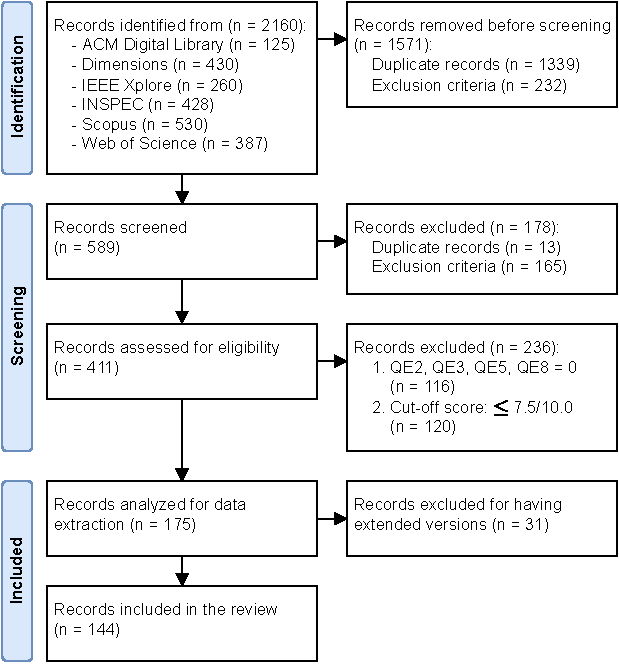
\includegraphics[width=\columnwidth]{figures/selection.pdf}
  \caption{PRISMA flow diagram for the selection process.}
  \label{fig:methodology:prisma-flow}
\end{figure}

\subsubsection{Identification}

In the identification phase of this review, the search strategy is applied to all data sources. \citetitle{methodology:search:db:acm}, \citetitle{methodology:search:db:dimensions}, \citetitle{methodology:search:db:inspec}, \citetitle{methodology:search:db:scopus}, and \citetitle{methodology:search:db:wos} data sources only require a single inquiry to obtain the search results.
Given the limitation of the \citetitle{methodology:search:db:ieee-xplore} for using wildcards mentioned in Section~\ref{sec:methodology:search}, the number of records for this source presented in Figure~\ref{fig:methodology:prisma-flow} represents the results of 7 inquiries (using the fields title, abstract, author keywords, IEEE terms, INSPEC controlled terms, and the INSPEC uncontrolled ones, respectively) after removing the duplicates with the support of Parsifal. Although the total number of search results found is 2160, Parsifal is used to remove duplicates from different data sources, excluding 1339 records. Following the duplicates removal, the exclusion criteria defined in Section~\ref{sec:methodology:search} exclude 232 works from the review. This exclusion is possible due to \citetitle{methodology:search:db:inspec}, \citetitle{methodology:search:db:scopus}, or \citetitle{methodology:search:db:wos} having filters related to the publication's type, subject area, and language.

The works excluded from the search results also include the ones that do not meet the exclusion criteria E4 and E7. For the first one, a Python script available in the GitHub repository of this review searches studies with a number of pages lower or equal to 4. Even though short papers have a maximum number of 3 pages, the papers with 4 pages do not usually present a detailed methodology.
As for the E7 exclusion criterion, some works are possible to remove from the review by searching in their title for the term ``dataset''.
All excluded articles of this review are double-checked to certify if the exclusion criteria are correctly applied. For example, articles published in the Remote Sensing journal from MDPI do not meet the E3 criterion. Indeed, the Journal Citations Reports from Clarivate classifies it by the following categories: Remote Sensing, Geosciences Multidisciplinary, Environmental Sciences, and Imaging Science \& Photographic Technology. However, most search results from this journal found in the identification phase are directly related to the topic of this review and the respective subject areas. Thus, in these cases and in other ones related to the remaining exclusion criteria, the decision is reverted to consider the initially rejected studies for the next phase of the review.

\subsubsection{Screening}

Next, the screening phase in this review consists of reading the title and abstract of the publications and rejecting the ones that meet the exclusion criteria. However, the initially rejected papers have another assessment for validating the exclusion. The analysis of the results and conclusions of these publications considering the exclusion criteria either confirms the exclusion decision or reverses it to eligible works for quality assessment. As a result of the screening phase, 178 studies are rejected from the initial identified 589 works. The duplicate records found in screening and removed manually are due to titles with invalid characters originated by exporting the search results from the \citetitle{methodology:search:db:dimensions}~database.

\subsubsection{Quality assessment}

The quality evaluation in this review of the selected works from screening follows the 8 Quality Evaluation (QE) criteria presented in Table~\ref{tab:methodology:quality-assessment}. All of them are subjective criteria derived from the analysis of the eligible works. The score column establishes the possible values for the QE criteria, in which the minimum, intermediate, and maximum values correspond to none, partial, and full compliance, respectively.
Furthermore, QE1, QE2, QE4, and QE8 focus on the details provided in the papers, specifically, if the discussion of the related work, the proposed methodology, the experimental setup, and the results are detailed and thoroughly analyzed in the publication, respectively.
The possible scores for QE3 are twice the value of QE1, QE2, QE4, and QE8 due to this criterion being directly related to the topic of the review. A work focusing on both localization and mapping problems will have a score of 2.0 (full compliance). If the study only focuses on one of these problems or none of them, the scores will be 1.0 or 0.0, i.e., partial or no compliance, respectively.
QE5 evaluates the long-term results of the eligible studies and is either 2.0 (full) or 0.0 (no compliance). This criterion has the same range as QE3 for similar reasons, given the focus of this review on long-term localization and mapping algorithms.
The definition of long-term experiments for assigning full compliance in QE5 is the following one: dynamic changing environments (e.g., dynamic elements or semi-static ones), increasing environments or feature maps in terms of their size, redundant data removal, or varying conditions (e.g., different seasons of the year or lighting conditions).
QE6 and QE7 can only be 1.0 or 0.0. The former criterion intends to highlight works that compare themselves to the state of the art and/or ground-truth data. The latter emphasizes the importance of having available either the implementation of the proposed methodology or the data used in the experiments for other works to be able to compare the proposed methodologies.
Lastly, considering the possible scores for the QE criteria in Table~\ref{tab:methodology:quality-assessment}, each work can only have a  maximum score of 10.0.

\begin{table}[h]
  \renewcommand{\arraystretch}{1.25}
  \setlength{\tabcolsep}{3pt}
  \caption[Quality evaluation criteria and score range.]{Quality evaluation criteria and score range.}
  \label{tab:methodology:quality-assessment}
  \centering
  {\scriptsize
  \begin{tabular}{c m{0.68\columnwidth} c}

\hline
\textbf{QE\#} & \textbf{Criteria} & \textbf{Score}\\
\hline
QE1 &
Does the paper have an updated state of the art on long-term localization and mapping? &
\{0.0, 0.5, 1.0\}\\
\hline
QE2 &
Is the methodology appropriate and detailed? &
\{0.0, 0.5, 1.0\}\\
\hline
QE3 &
Does the methodology consider both localization and mapping problems? &
\{0.0, 1.0, 2.0\}\\
\hline
QE4 &
Is the hardware and/or software used in the experiments detailed? &
\{0.0, 0.5, 1.0\}\\
\hline
QE5 &
Does the paper presents any kind of long-term experimental results? &
\{0.0, 2.0\}\\
\hline
QE6 &
Does the paper presents comparative results with other methods and/or ground-truth data? &
\{0.0, 1.0\}\\
\hline
QE7 &
Does the work's implementation and/or the data used in the experiments are publicly available? &
\{0.0, 1.0\}\\
\hline
QE8 &
Is the discussion of the results and conclusions appropriate and detailed? &
\{0.0, 0.5, 1.0\}\\
\hline

  \end{tabular}}
\end{table}

After evaluating the 411 eligible works accordingly to the previously discussed QE criteria (the scores of each record are available in the GitHub repository), the first conclusion of the authors is that works with a non-detailed or not appropriate methodology, results' discussion, or conclusions should not be included in the review. Another conclusion is relative to rejecting works that do not consider either localization or mapping problems, or do not present any long-term experimental results, given the focus of this review on the long-term localization and mapping problem for mobile robots. Furthermore, the quality assessment phase should consider a cut-off score to filter works with low quality scores. Consequently, the assessment phase considers the following two reasons to reject a record:

\begin{enumerate}\setlength\itemsep{-0.5em}
\item QE2, QE3, QE5, QE8: reject works with a 0.0 (no compliance) score;
\item cut-off score: reject works with a score lower or equal to 7.5/10.0.
\end{enumerate}

The distribution of the evaluation scores and the QE criteria itself justify the selection of a 7.5/10.0 cut-off score. 
Figure~\ref{fig:methodology:qe} illustrates the scores distribution for all eligible works versus the scores of the ones that pass the first criterion defined previously for the QE phase (related to the compliance on the QE2, QE3, QE5, and QE8 criteria). The assessment of this criterion rejects 116 records (28\%) of the 411 eligible works (see Figure~\ref{fig:methodology:prisma-flow}). 
Even though the distribution of the evaluation scores changes significantly in the range of scores lower or equal to 7.5/10.0, as observed between Figures~\ref{fig:methodology:qe:qe_wo-r1} and~\ref{fig:methodology:qe:qe}, only one work with a score higher than 7.5 is rejected due to not having a detailed and appropriate discussion of the results. This result indicates that interesting works are associated with high scores, as intended when using a quality assessment methodology, while also suggests that the range between 8.0 and 10.0 have the most interesting and quality works compatible with the focus of this review on long-term localization and mapping. Although only assessing the eligible works would seem to lead to the same results in terms of records included in the review, the rejection criterion on QE2/3/5/8 prevents outliers related to the quality assessment.
From the remaining 295 eligible works, cut-off scores from 7.5 up to 8.5 have the following corresponding rejection rates:

\begin{itemize}[nosep]
\item 7.5/10.0 \phantom{$\xrightarrow{\text{reject}}$} 120 records (40.7\%) \phantom{$\xrightarrow{\text{include}}$} 175 records
\item 8.0/10.0 $\xrightarrow{\text{reject}}$ 160 records (54.2\%) $\xrightarrow{\text{include}}$ 135 records
\item 8.5/10.0 \phantom{$\xrightarrow{\text{reject}}$} 203 records (68.8\%) \phantom{$\xrightarrow{\text{include}}$} 92 records
\end{itemize}

\begin{figure}[h]
  \centering
  \subfloat[][]{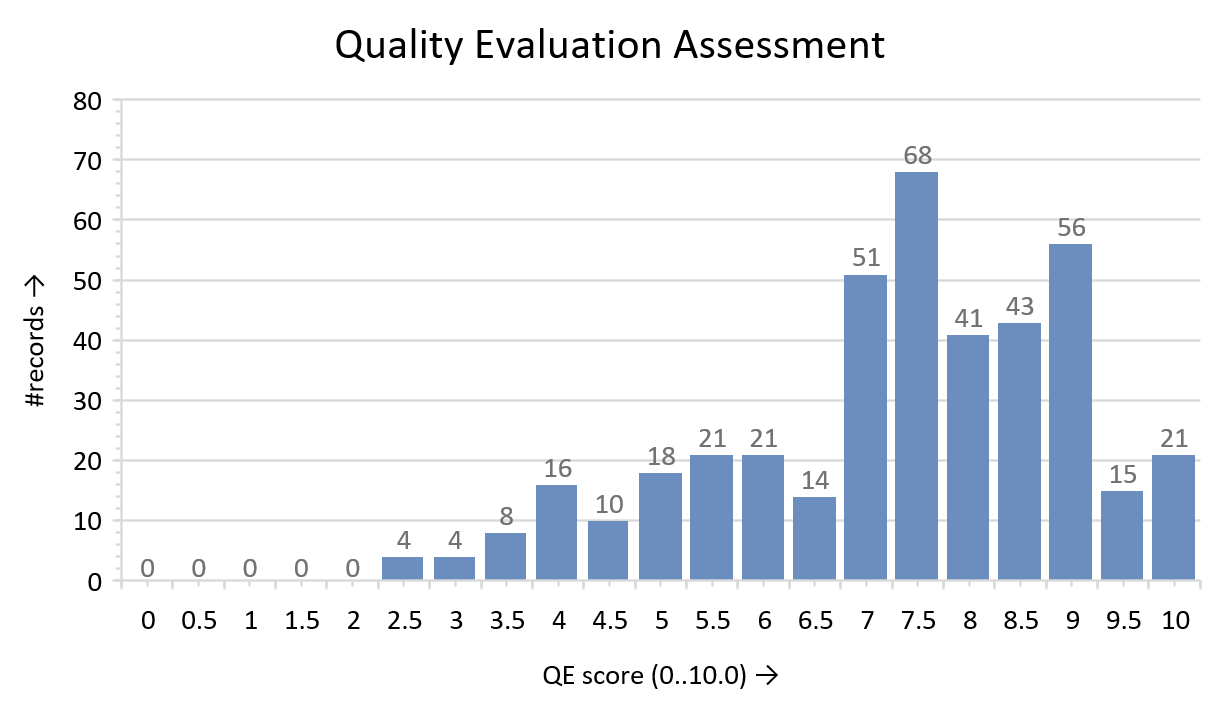
\includegraphics[width=\columnwidth]{figures/qe.png}%
  \label{fig:methodology:qe:qe}}
  \linebreak
  \subfloat[][]{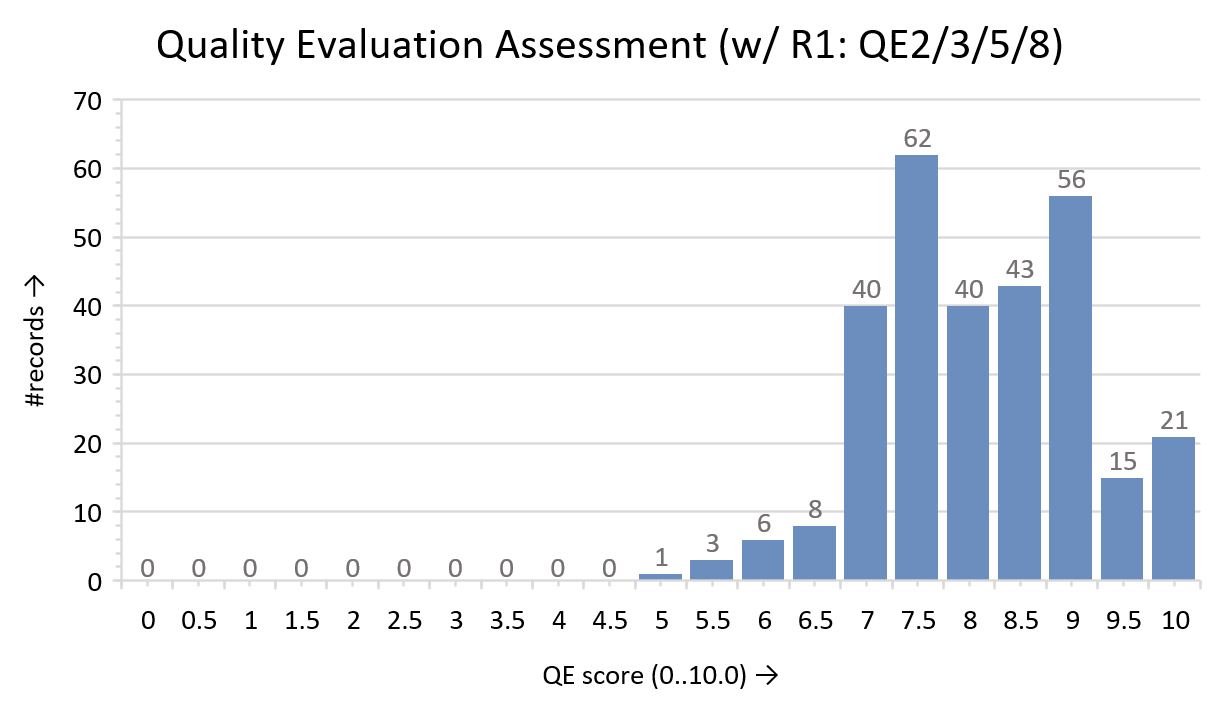
\includegraphics[width=\columnwidth]{figures/qe_wo-r1.png}%
  \label{fig:methodology:qe:qe_wo-r1}}
  \caption{Distribution of the quality evaluation scores obtained from assessing the eligible works considered in the review: (a) all eligible works; (b) works that pass the rejection criterion during the QE assessment related to QE2/3/5/8 = 0.0 (no compliance).}
  \label{fig:methodology:qe}
\end{figure}

The 8.5 cut-off score would not be suitable because methods that focus only on localization or mapping, or not having either the implementation or the experimental data publicly available would be obligated to have maximum scores in the other criteria to be included in the review. In these cases, a work would have a maximum score of 9.0 due to partial compliance on QE3 or no compliance on the QE7 criteria. Likewise, a cut-off score of 8.0 would only leave a margin for having a single partial compliance on QE1, QE2, QE4 or QE8 criteria in similar cases, even though it would reject 160/295 (54\%) records. Therefore, the 7.5/10.0 cut-off score is more appropriate for the quality assessment phase in this review by leaving margin for works to have partial compliance in more than one criterion. Indeed, this cut-off score allows an article with no public data and/or implementation (e.g., due to confidentiality agreements) to have up to four criteria with partial compliance, depending on the criterion's maximum score or if the work has available the experiments data and/or implementation. Another example is articles that only focus on localization or mapping. In these cases, the work could have no public implementation, even though requiring a maximum score on all other criteria, or, if the work has public data or implementation available, two other criteria could have partial compliance.

Overall, as illustrated in Figure~\ref{fig:methodology:prisma-flow}, the quality assessment of the 411 eligible works considering the two rejection criteria previously mentioned leads to rejecting a total of 236 (57\%) records. As a result, the remaining 175 records will be analyzed for data extraction.

\subsection{Data extraction}
\label{sec:methodology:data}

The data extraction process analyzes the records selected after the quality assessment phase and extracts information from these works. In the scope of this review, the Data Extraction (DE) items required for each record are the following ones:

\begin{itemize}[nosep]
\item $\left[\textbf{DE1}\right]$ \textbf{Long-term considerations} -- long-term factors the works consider in their proposed approach and experiments. Considering the knowledge obtained in the previous phases of this review's methodology, the authors considered the following factors for categorizing the included works:
  \begin{itemize}[nosep]
  \item appearance: varying conditions, appearance changes;
  \item dynamics: environment dynamics, dynamic elements;
  \item sparsity: map pruning, redundant data removal;
  \item multi-session: map management;
  \item computational: memory management, efficiency.
  \end{itemize}
\item $\left[\textbf{DE2}\right]$ \textbf{Localization} -- how the robot localizes itself and the type of localizer;
\item $\left[\textbf{DE3}\right]$ \textbf{Mapping} -- type of the map;
\item $\left[\textbf{DE4}\right]$ \textbf{Multi-robot} -- if the proposed methodologies consider multi-robot systems;
\item $\left[\textbf{DE5}\right]$ \textbf{Execution mode} -- offline, online, if requires both, or if no information on this item;
\item $\left[\textbf{DE6}\right]$ \textbf{Environment and domain} -- type of environment (indoor, outdoor) and domains (air, ground, water) tested with the proposed methodologies;
\item $\left[\textbf{DE7}\right]$ \textbf{Sensory setup} -- which sensors considered in the methodologies;
\item $\left[\textbf{DE8}\right]$ \textbf{Non-public experiments} -- if the authors performed experiments or tests with non-public data;
\item $\left[\textbf{DE9}\right]$ \textbf{Ground-truth} -- how ground-truth for non-public data is obtained or its type, if available;
\item $\left[\textbf{DE10}\right]$ \textbf{Distance and time characteristics} -- relative to the non-public experiments if available, as follows:
  \begin{itemize}[nosep]
  \item total distance (km) of the non-public experiments;
  \item path (km), in the case of repetitive paths;
  \item total time (h) in terms of continuous operation;
  \item time interval (day/week/month/year, or d/w/m/y) between the first and the last run.
  \end{itemize}
\item $\left[\textbf{DE11}\right]$ \textbf{Datasets} -- if and which public datasets are used in the experiments;
\item $\left[\textbf{DE12}\right]$ \textbf{Evaluation metrics} -- which metrics are used for evaluation.
\end{itemize}

In Section~\ref{sec:discussion}, a comparison table of the public datasets identified by the DE11 will contain the sensory setup, ground-truth data availability from the datasets, and the distance and time characteristics, similar to the data extraction items for non-public data, among other aspects. As a result, the distinction between public and non-public data availability represented in DE8, DE9, and DE10 allows to understand the distance and time characteristics of non-public data independently from the public datasets.

Although the data extraction phase in a systematic literature review usually does not remove any records, 31 of the analyzed 179 works have extended versions of the proposed methodologies, more detailed ones, or equivalent methods applied in different conditions.
Thus, these records are not included in the review to improve the discussion section in terms of singularity and originality of proposed approaches for the long-term localization and mapping problem.
The extracted information helped identifying the corresponding extended and more complete versions of these works.
A document containing the association of the removed versions to the records included in the review is available in the public GitHub repository, including their bibliographic references. 

Consequently, 144 original works are included in this review for an overview of these records in Section~\ref{sec:overview}, and their synthesis and discussion in Section~\ref{sec:discussion}. The information relative to the 12 data items for each of the included records is available in Appendix~\ref{a2:data-extraction} and also in the repository. The included works represent 35\% of the 411 eligible records for this review. This result indicates that the methodology followed in this review led to a high percentage of quality results.


\section{Results Overview}
\label{sec:overview}

In this section, the main goal is to overview the results not in terms of their scientific contribution but in terms of their bibliographic data for presenting an overview of the included records in the review. First, statistic results of the data sources in which the 142 included records could be identified in the methodology allow the evaluation of the coverage between the sources.
Next, the tool VOSviewer~\parencite{results:vosviewer:1,results:vosviewer:2} is used to obtain the co-occurrence analysis for the keywords and the authors. The former focus on the keywords recency and their occurrence in the sources, while the latter discusses the research networks between the authors, and the ones with more publications in long-term localization and mapping.
Lastly, two analysis are presented relative to the evolution of the publication year and most relevant publication venues.

\subsection{Data source}
\label{sec:overview:db}

The results on the identification phase are exported to BibTeX files from each data source. This exportation considers all the information available in the data sources, such as citation (e.g., author, title, publication venue, and type of record) and bibliographic (e.g., affiliation and the publisher) information of each record, the abstract, and author and indexed keywords. Next, using the \texttt{bibtexparser}\footnote{\url{https://bibtexparser.readthedocs.io/en/master/}} Python library, the BibTeX files are processed to identify uncompleted records. For example, the DOI must be specified and, if not available, the record's information must be manually completed with a corresponding URL. Then, considering the 142 included records in this review, a Python script searches each record in the BibTeX files corresponding to each data source. This search uses the DOI, URL, and title data to identify if a data source had in its identification results the searched record. Given that these three fields can contain lower and upper letters, the respective strings must be compared only after converting them to lower cases. As a result, the number of identified records by each data source of the 142 included ones in the review are the following ones:

\begin{itemize}[nosep]
\item \citetitle{methodology:search:db:acm}: 25 records (17.6\%);
\item \citetitle{methodology:search:db:dimensions}: 84 records (59.2\%);
\item \citetitle{methodology:search:db:ieee-xplore}: 67 records (47.2\%);
\item \citetitle{methodology:search:db:inspec}: 102 records (71.8\%);
\item \citetitle{methodology:search:db:scopus}: 120 records (84.5\%);
\item \citetitle{methodology:search:db:wos}: 105 records (73.9\%).
\end{itemize}

The database \citetitle{methodology:search:db:scopus} is the source that identified the greatest number of included records. This result was expected given that \citetitle{methodology:search:db:scopus} is considered as one of the largest curated databases~\parencite{methodology:search:db:coverage:dim-scopus-wos}, indexing more than 25000 active titles (e.g., conferences proceedings, journals) and 7000 publishers\footnote{\url{https://www.elsevier.com/solutions/scopus/how-scopus-works}}.
Two other sources with more than 70\% of identified records are \citetitle{methodology:search:db:inspec} and \citetitle{methodology:search:db:wos}. Similarly to \citetitle{methodology:search:db:scopus}, these two databases index also records from thousands of journals, conferences, and publishers\footnote{\url{https://www.elsevier.com/solutions/engineering-village/content/inspec}}\textsuperscript{,}\footnote{\url{https://clarivate.com/webofsciencegroup/solutions/web-of-science/}}.
Although \citetitle{methodology:search:db:dimensions} is also a bibliographic database covering millions of publications from thousands of sources, this database is the newest one (created in 2018) relative to the other three considered in this review (\citetitle{methodology:search:db:inspec}, \citetitle{methodology:search:db:scopus}, and \citetitle{methodology:search:db:wos}) and could be a factor to why it obtained a lower percentage (59.2\%) than the other three databases. Another possible reason is that \citetitle{methodology:search:db:scopus} and \citetitle{methodology:search:db:wos} have the majority of their coverage in Life Sciences, Physical Sciences, and Technology Area (including the Engineering subject area related to the topic of this review), while \citetitle{methodology:search:db:dimensions} has better coverage in Social Sciences and Arts \& Humanities~\parencite{methodology:search:db:coverage:dim-scopus-wos}.
Even though \citetitle{methodology:search:db:ieee-xplore} is a digital library and only indexes works published by IEEE and its partners, this data source returns 47.2\% of the include records in the review. The main reason is that this library indexes publications related to electrical engineering and computer science, subject areas related to long-term localization and mapping\footnote{\url{https://ieeexplore.ieee.org/Xplorehelp/overview-of-ieee-xplore/about-ieee-xplore}}.
Finally, the \citetitle{methodology:search:db:acm} using \textit{The ACM Guide to Computing Literature} collection only finds published records by ACM and possible links to other records focused exclusively on computing\footnote{\url{https://libraries.acm.org/digital-library/acm-guide-to-computing-literature}} and not directly related to the Computer Science or Engineering subject areas, explaining why this source obtained a lower coverage percentage of the included results than the other sources for this review.

Furthermore, Table~\ref{tab:overview:source} presents a coverage analysis of the identified results from each data source for the 142 included records in this review. Table~\ref{tab:overview:source:intersect} presents the pairwise overlap between sources. The corresponding percentage is the ratio of records identified by both sources to the one between the two that has the smallest number of results: $\#\{A\cap B\} / \text{min}\{\#A,\#B\}$, where $\#A$ and $\#B$ is the number of results for a data source $A$ and $B$, respectively, and $\#\{A\cap B\}$ is the intersection results between the two sources. For example, if the pairwise results is 100\%, it means that the data source with more records found was capable of obtaining all the results, i.e., had full coverage over the other source. Table~\ref{tab:overview:source:union} reports the percentage of records identified by at least one of two data sources over all 142 included records: $\#\{A\cup B\} / 142$, where $A\cup B$ is the union correspondence results of the sources $A$ and $B$. This percentage represents the joint coverage of two databases over the 142 included records.
					
\begin{table}[h]
  \centering
  \caption{Pairwise coverage analysis of the data sources considered in the review over the 142 included records: (a) identification only on both pairwise sources ($\#\{A\cap B\} / \text{min}\{\#A,\#B\}$); (b) on either ones ($\#\{A\cup B\} / \#\text{records}$). Legend: dim -- \citetitle{methodology:search:db:dimensions}, ieee -- \citetitle{methodology:search:db:ieee-xplore}, insp -- \citetitle{methodology:search:db:inspec}, scop -- \citetitle{methodology:search:db:scopus}, wos -- \citetitle{methodology:search:db:wos}.}
  \label{tab:overview:source}
  \subfloat[][]{%
  \label{tab:overview:source:intersect}%
  \begin{tabular}{l|P{0.08\columnwidth}P{0.08\columnwidth}P{0.08\columnwidth}P{0.08\columnwidth}P{0.08\columnwidth}P{0.08\columnwidth}}
\hline
$A\cap B$ & \textbf{acm} & \textbf{dim} & \textbf{ieee} & \textbf{insp} & \textbf{scop} & \textbf{wos}\\
\hline
\textbf{acm}  & -- & 96.0\% & 44.0\% & 88.0\% & 96.0\% & 96.0\%\\
\textbf{dim}  & -- & --     & 68.7\% & 77.4\% & 97.6\% & 96.4\%\\
\textbf{ieee} & -- & --     & --     & 89.6\% & 91.0\% & 74.6\%\\
\textbf{insp} & -- & --     & --     & --     & 87.3\% & 69.6\%\\
\textbf{scp}  & -- & --     & --     & --     & --     & 89.5\%\\
\textbf{wos}  & -- & --     & --     & --     & --     & --\\
\hline
    \end{tabular}%
  }
  \linebreak
  \subfloat[][]{%
  \label{tab:overview:source:union}%
  \vspace{0.5em}
  \begin{tabular}{l|P{0.08\columnwidth}P{0.08\columnwidth}P{0.08\columnwidth}P{0.08\columnwidth}P{0.08\columnwidth}P{0.08\columnwidth}}
\hline
$A\cup B$ & \textbf{acm} & \textbf{dim} & \textbf{ieee} & \textbf{insp} & \textbf{scop} & \textbf{wos}\\
\hline
\textbf{acm}  & -- & 59.9\% & 57.0\% & 73.9\% & 85.2\% & 74.6\%\\
\textbf{dim}  & -- & --     & 73.9\% & 85.2\% & 85.9\% & 76.1\%\\
\textbf{ieee} & -- & --     & --     & 76.8\% & 88.7\% & 85.9\%\\
\textbf{insp} & -- & --     & --     & --     & 93.7\% & 95.8\%\\
\textbf{scp}  & -- & --     & --     & --     & --     & 92.3\%\\
\textbf{wos}  & -- & --     & --     & --     & --     & --\\
\hline
  \end{tabular}%
  }
\end{table}

Analyzing the coverage results in Table~\ref{tab:overview:source}, the first observation is that the pairwise union results of two sources increase the independent coverage of each source. This observation validates the need identified in the methodology discussed in Section~\ref{sec:methodology} to consider several data sources in the identification phase of a review. Moreover, the pairwise union coverage of \citetitle{methodology:search:db:inspec}, \citetitle{methodology:search:db:scopus}, and \citetitle{methodology:search:db:wos} is greater than 90\% of the included records. When evaluating the joint coverage of these three databases, they identify all 142 of the included records, i.e., a 100\% coverage. Although this result could indicate that those three sources guarantee full coverage of the long-term localization and mapping research topic, it is always advisable to consider as most as possible sources in the methodology. Another observation is relative to the overlap of \citetitle{methodology:search:db:scopus} with the other sources, which is greater than 85\%. This overlap indicates that \citetitle{methodology:search:db:scopus} covers results not only on the topic of this review but also the results obtained by the other sources considered in the methodology. Lastly, \citetitle{methodology:search:db:inspec} and \citetitle{methodology:search:db:wos} achieve a pairwise overlap percentage of 69.6\% between themselves, while their union represents 95.8\% of the included records. This discrepancy indicates that these two sources identify unique results between themselves. Indeed, \citetitle{methodology:search:db:inspec} identifies 31/142 records not found by \citetitle{methodology:search:db:wos}, and vice-versa for \citetitle{methodology:search:db:wos}, with 34/142 unique records.

\subsection{Keywords co-occurrence}
\label{sec:overview:kw}

Next, VOSviewer~\parencite{results:vosviewer:1,results:vosviewer:2} is used to analyze the co-occurrence of keywords in the included articles. This co-occurrence is the relatedness of items determined based on the number of documents in which the keywords occur together.
For this analysis, first, a Python script processes the BibTeX file containing the citation and bibliographic information, the author and the indexed keywords, and the abstract of the records to join the author with the indexed keywords in the same \texttt{keywords} field. Then, an online tool\footnote{\url{https://www.bibtex.com/c/bibtex-to-ris-converter/}} converts this processed BibTeX to a RIS file.
Even though VOSviewer supports file types directly exported from \citetitle{methodology:search:db:dimensions}, \citetitle{methodology:search:db:scopus}, or \citetitle{methodology:search:db:wos} as input, none of these data sources obtained all the 142 included records of the review in the identification phase. Given that VOSviewer does not support BibTeX files, the conversion to RIS file is required for using as input.
The disadvantage of using this file format in VOSviewer is only allowing to perform co-occurrence of items (e.g., keywords or authors), while bibliographic data from \citetitle{methodology:search:db:dimensions}, \citetitle{methodology:search:db:scopus}, or \citetitle{methodology:search:db:wos} in CSV files would allow other analysis such as citation, co-citation, or bibliographic coupling.
However, the creation of these CSV files follow different templates depending on the data source. So, RIS files allow the integration of all 142 included records for obtaining the two co-occurrence analysis presented in this review (namely, keywords and co-authorship).

In Figure~\ref{fig:overview:kw:original}, the network presents the overlay visualization of the keywords co-occurrence in the included records weighted by the number of occurrences of each term, using full counting for the links' strength. The latter computes the strength of the links directly by the number of co-occurrences of the respective two terms.
The overlay visualization colors the keywords differently according to the average publication year of the included records in which each of the keywords appears. This coloring allows analyzing which are the ones that are associated with the most recent publications.
As for the keywords' weighting, the number of occurrences dictates the size of the circles.
Furthermore, the minimum number of occurrences of a keywords set in VOSviewer for obtaining the graph is 5 originating the 34 keywords illustrated in Figure~\ref{fig:overview:kw:original}. This parameter was selected for visualization purposes while also filtering uninteresting keywords.
Similarly, setting the attraction and repulsion parameters to 2 and 0, respectively, distances the terms more from each other than using the values recommended in the VOSviewer manual\footnote{\url{https://www.vosviewer.com/documentation/Manual_VOSviewer_1.6.8.pdf}} (2 and 1, respectively). These two parameters only interfere in the localization of the terms in the map, not in the graph connections.
Lastly, a thesaurus of the keywords (available in the repository) is used to join similar terms: spelling differences (e.g., localization -- localisation), full terms versus abbreviations (simultaneous localization and mapping -- SLAM), while also allowing the concatenation of long keywords for visualization reasons.

\begin{figure*}[!t]
  \centering
  \subfloat[][]{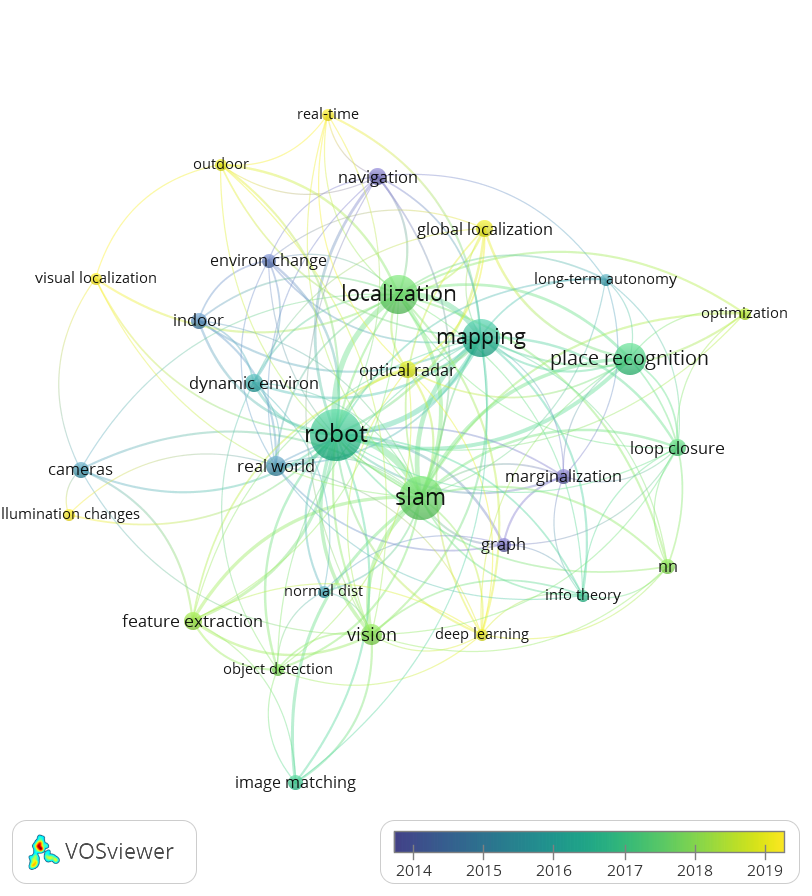
\includegraphics[width=\columnwidth]{figures/kw.png}%
  \label{fig:overview:kw:original}}
  \hfill
  \subfloat[][]{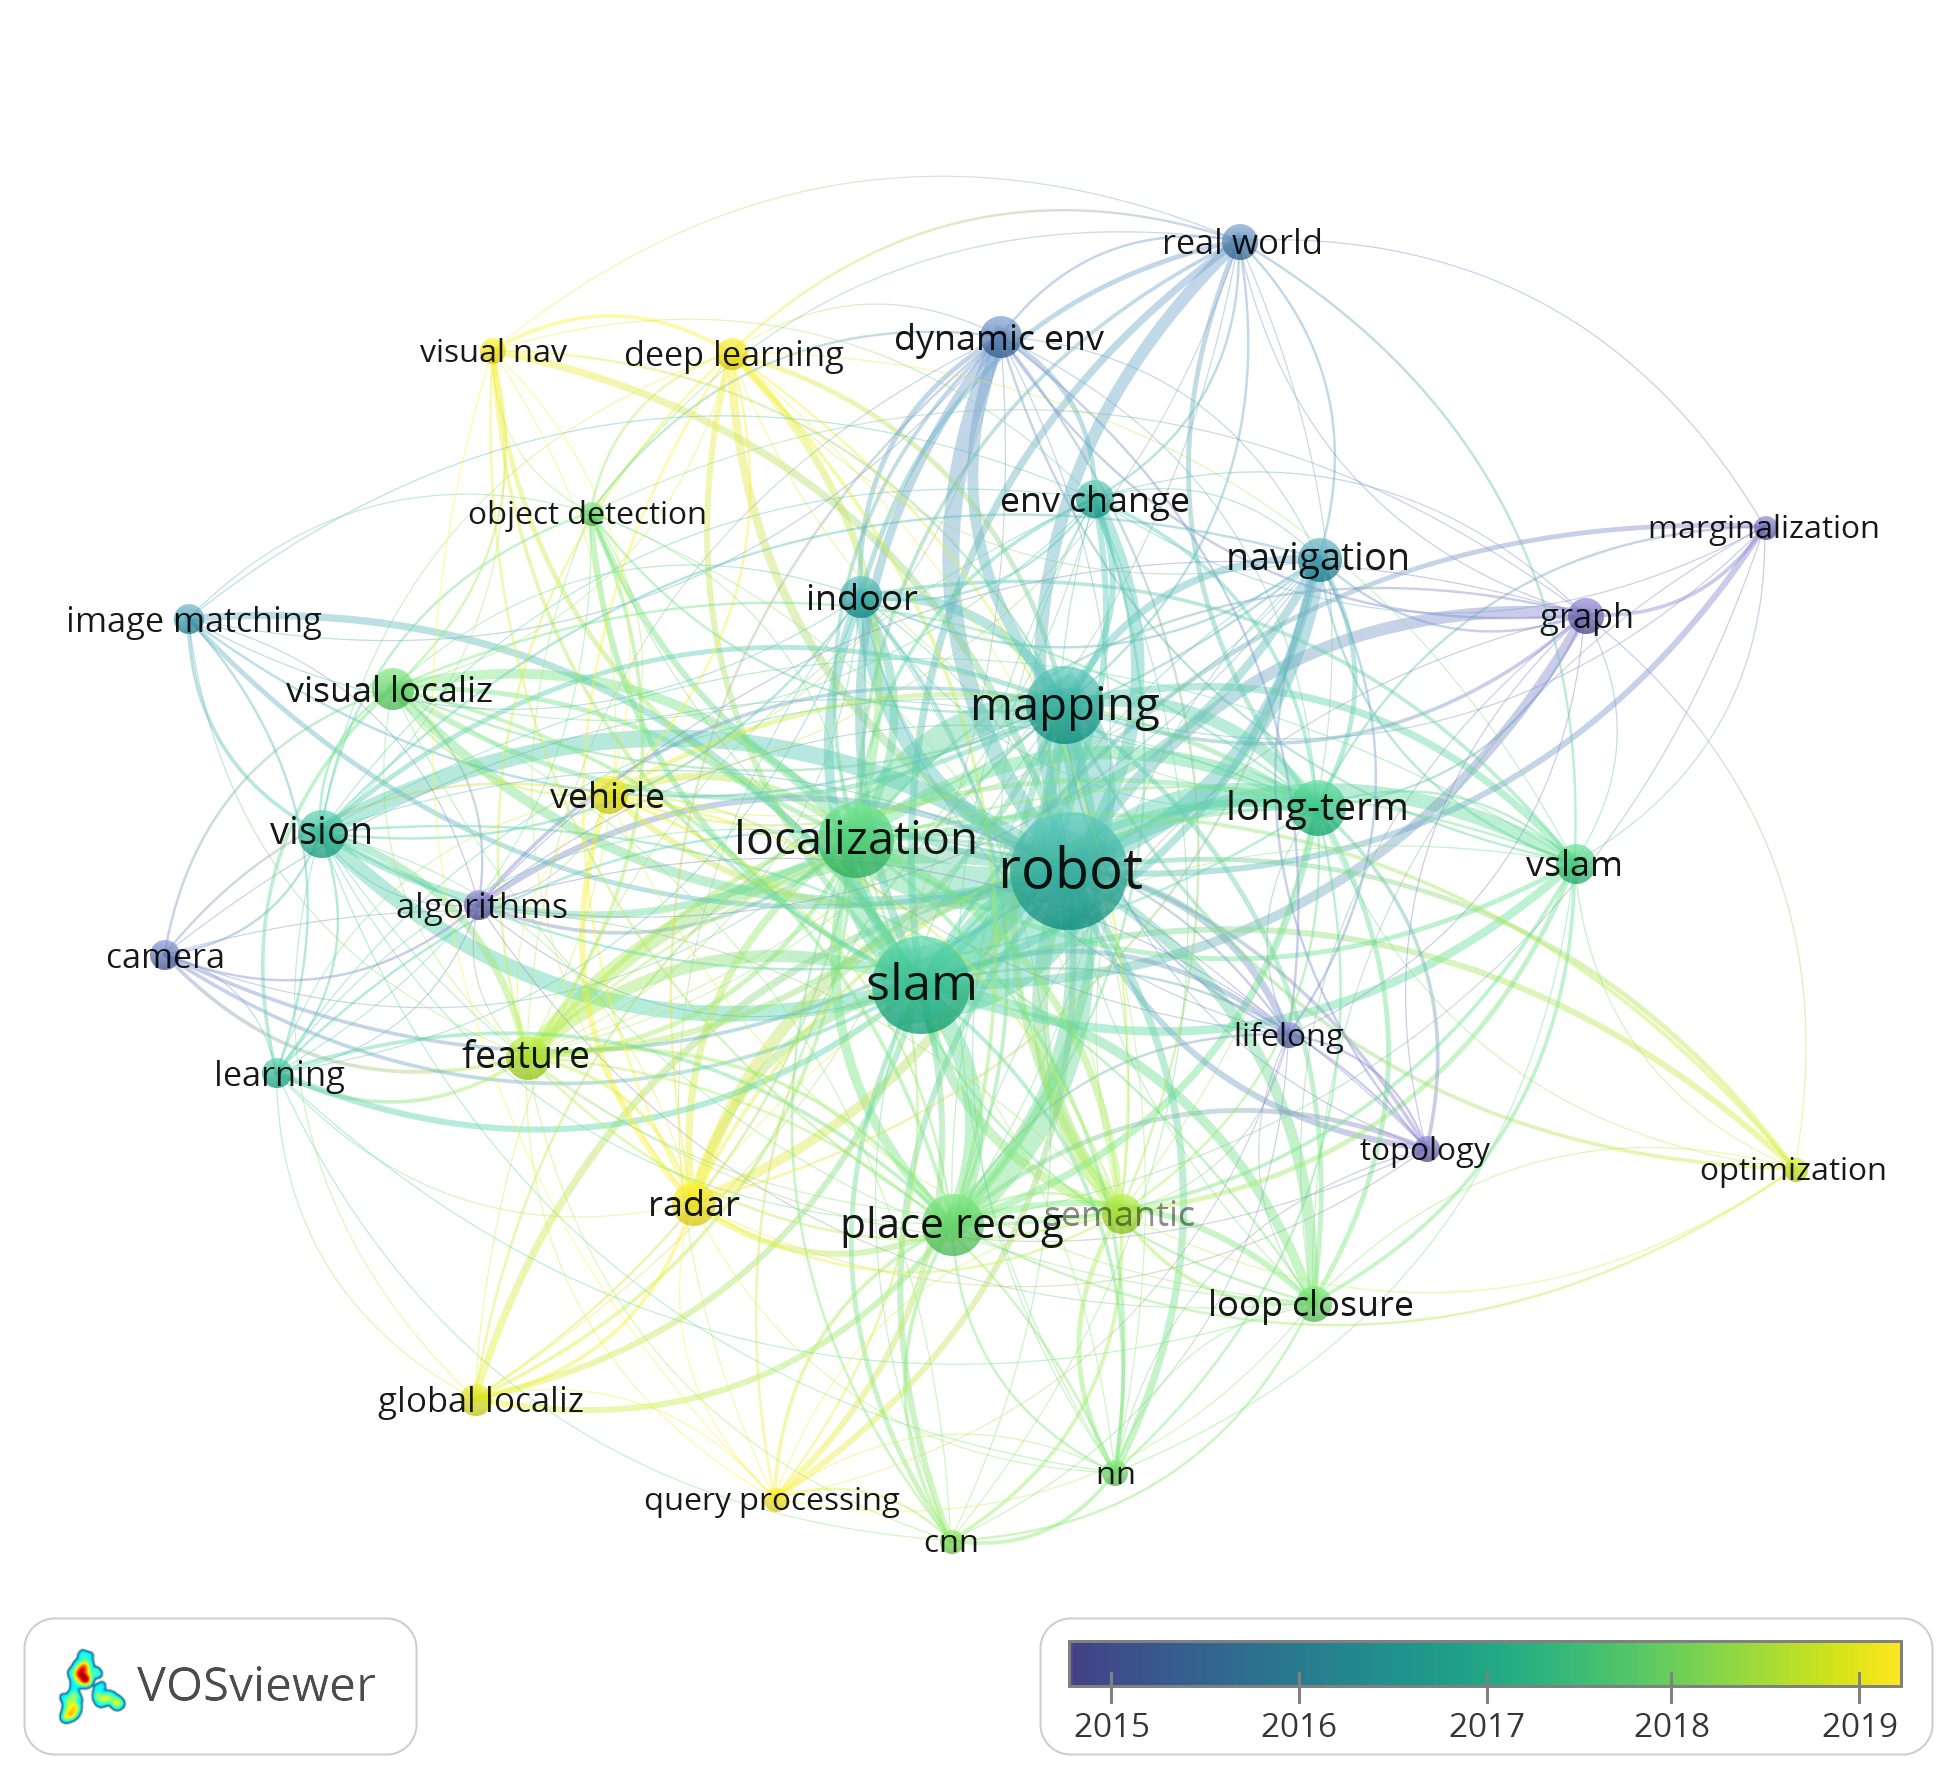
\includegraphics[width=\columnwidth]{figures/kw_long-term.png}%
  \label{fig:overview:kw:long-term}}
  \caption{Keywords co-occurrence analysis on the 142 included records generated by VOSviewer with overlay visualization by the average publication year: (a) original keywords; (b) all keywords containing long-term and lifelong summarized by the terms themselves. Parameters used for generating the co-occurrence network: minimum number of occurrences = 5, attraction = 2, repulsion = 0, scale = 1.49, circles size variation = 0.5, lines size validation = 1.0. Legend: \texttt{cnn} -- Convolutional Neural Networks, \texttt{env} -- environment, \texttt{localiz} -- localization, \texttt{nav} -- navigation, \texttt{nn} -- Neural Networks, \texttt{recog} -- recognition, \texttt{vslam} -- visual SLAM.}
  \label{fig:overview:kw}
\end{figure*}

Overall, the keyword \texttt{robot} is the one that appears more times in the included records: 109 occurrences, links with 33 other terms, and has a total link strength of 390 (sum of co-occurrences of all of its links). This result is expected due to the relation of this review's topic to robotics.
Similarly, three other keywords in the network related to long-term localization and mapping topic with high values of occurrence, number of links, and total link strength are \texttt{slam} (74, 33, and 280), \texttt{mapping} (47, 32, and 196), and \texttt{localization} (46, 31, and 188, respectively). The methodology for the search strategy discussed in Section~\ref{sec:methodology:search} considers all of these four keywords. Thus, the significant influence of \texttt{robot}, \texttt{slam}, \texttt{mapping}, and \texttt{localization} in the keywords co-occurrence analysis indicates that, after the all the phases executed in this review's methodology, the 142 included records have a high correlation with the keywords considered in the search query. Given that the keywords are usually selected or indexed to capture the essence of the document, this correlation indicates that the search query is appropriate to obtain the search results, even considering only the keywords as search fields.

As for keywords related to the outcome of the PICO framework, \texttt{long-term autonomy} occurs only 6 times in the included records, linking with 16 other keywords and having a total link strength of 27. This low occurrence could indicate that the term \texttt{long-term autonomy} is not usually used by the authors nor indexed by the databases. 
However, the specific term of \texttt{long-term autonomy} does not summarize all the possibilities for the outcome of the PICO framework (see Section~\ref{sec:purpose}). Indeed, for this reason, the search query for the identification phase uses only the following single terms: \texttt{"long term"} and \texttt{"life long"} (resumes the possibility of having a space or a hyphen), and \texttt{lifelong}.
Figure~\ref{fig:overview:kw:long-term} presents the keywords co-occurrence analysis using the same parameters for obtaining Figure~\ref{fig:overview:kw:original}. The difference to the latter network is using a thesaurus that summarizes all the keywords that contain \texttt{long-term} and \texttt{lifelong} into the terms themselves, obtaining 35 keywords with a minimum of 5 occurrences in the 142 included records.
In terms of occurrences, number of links, and total link strength, the impact of the thesaurus keyword \texttt{long-term} is 25, 27, and 103, and for lifelong 6, 17, and 31, respectively. These values are much higher than the ones respective only to \texttt{long-term autonomy} from Figure~\ref{fig:overview:kw:original}.
The reason is that \texttt{long-term} in Figure~\ref{fig:overview:kw:long-term} compiles the occurrences of keywords such as \texttt{long-term autonomy}, \texttt{long-term mapping}, and \texttt{long-term localization} (6, 2, and 2 occurrences, respectively), and \texttt{lifelong} sum up, for example, three different versions of \texttt{lifelong learning} (using \texttt{lifelong}, \texttt{life-long} and \texttt{life long} with 2, 1, and 2 occurrences, respectively) and \texttt{lifelong slam} (1 occurrence). Hence, these results proves that the third \texttt{AND} part of the search query (\texttt{"long term" OR "life long" OR lifelong}) covers well the PICO framework's outcome. Plus, they also show no consensus among the authors and by the databases indexation on how to define a keyword for the topic of long-term localization and mapping.

In terms of the average year of publication, analyzing the diagrams in Figure~\ref{fig:overview:kw} on its colorization, the first observation is the recency of terms related to visual localization. The keywords visual SLAM (\texttt{vslam}), visual navigation (\texttt{visual nav}), and visual localization (\texttt{visual localiz}) have all an average publication year higher than 2017. This recency indicates that recent approaches related to the topic of this review, long-term localization and mapping, are more inclined to use vision as a sensorization input.
Another sensor that appeared with high relevance in the network is \texttt{radar}, with 15 occurrences and an average publication year of 2019.20. This sensor is agnostic to the environment changes such as illumination and season changes intrinsically associated with vision and could be the reason why the recent works related to long-term localization and mapping are using it.
Moreover, place recognition (\texttt{place recog}) stands out not only by its recency but importance. The keyword itself (\texttt{place recog}) occurs 31 times and an average publication year of 2017.77, with terms related to place recognition such as \texttt{loop closure} and global localization (\texttt{global localiz}) with recent average publication years (2017.82 and 2018.75, respectively) and strong link to place recognition (5 co-occurrences for each of the links between \texttt{loop closure} and \texttt{global localiz} with \texttt{place recog}). Lastly, machine learning also seems to be used in recent works included in this review. The keywork learning occurs 7 times with an average publication year of 2017.00. Neural Netowrks (\texttt{nn}), Convolutional Neural Networks (\texttt{cnn}), and \texttt{deep learning} have a similar number of occurrences (6, 5, and 8) and publication years higher than 2017 (2017.83, 2018.00, and 2019.12, respectively). These results could mean another trend of using machine learning to improve the long-term autonomy of mobile robots.

Although the recency of keywords related to dynamic environments is lower than 2017 (2015.50 and 2016.75 for \texttt{dynamic env} and \texttt{env change}), they have a high occurrence (14 and 12, respectively), located close to each other in the network, and have a strong link between them (4 co-occurrences). Three keywords also located near each other are \texttt{graph} and \texttt{marginalization} while having similar average publication years (2014.70 and 2014.60, respectively). Even though the number of occurrences of these terms is low (10 and 5 for \texttt{graph} and \texttt{ marginalization}, respectively), their map proximity could indicate a focus in the past on the topic of graph sparsity, i.e., maintaining the graph in the long-term to only depend on the environment size and not on the robot's operation time.

The keywords co-occurrence analysis also relates to the categories of DE1 (see Section~\ref{sec:methodology:data}). Works associated with place recognition, global localization, and loop closure terms require invariance to the appearance changes in the environment, equivalent to the appearance category. The dynamics category is associated with works focused on dynamic environments. As for the other group of keywords with a high occurrence and strong links between each other, the ones related to graph and marginalization, the respective works focus on removing uninformative data from the map~\parencite{kretzschmar-stachniss:2012:0278364912455072}, which is related to map sparsification, and so, to the sparsity category of DE1. These relations between the appearance, dynamics, and sparsity categories to the semantic analysis of the keywords co-occurrence supports the categorization of DE1 considered in this review, while also indicating that the discussion on the proposed methodologies should focus on each one of the categories. Even though the two remaining categories of DE1 (multi-session and computational) are not represented in the keyword analysis, the execution of the data extraction phase identified the need for having these two categories, given the importance of multi-session handling and computational efficiency for long-term localization and mapping. However, each category of DE1 will be discussed in Section~\ref{sec:discussion} in further detail.


\subsection{Co-authorship analysis}
\label{sec:overview:authors}

The other analysis obtained using VOSviewer is the co-authorship network presented in Figure~\ref{fig:overview:authors}. Similar to the keywords network illustrated in Figure~\ref{fig:overview:kw}, the co-occurrence of the authors' names creates links among them in the graph. The strength of these links is dictated by the number of documents the two authors of a link are co-authors in the same record, and the number of co-authored works determines the size of the circles respective to each author in the graph. 
In contrast to Figure~\ref{fig:overview:kw}, the network in Figure~\ref{fig:overview:authors} does not have any overlay specific to coloring depending on the average publication year. Instead, the main goal of the co-authorship analysis in this review is to present possible research networks detected in the 142 included records. Thus, the coloring in Figure~\ref{fig:overview:authors} represents the clusters of authors detected by VOSviewer. This network only considers authors with a minimum of 3 works for relevance and visualization reasons, resulting in 27 authors.
Also, authors identified only by the initial of the first name and by the surname can lead to incorrect correspondences in terms of co-authorship. VOSviewer detects 392 authors in the 142 included records using the original RIS file used in Section~\ref{sec:overview:kw} compared to 413 after checking the authors names. Indeed, a manual check is performed on all authors of the included records to guarantee no false correspondences for the co-authorship analysis with VOSviewer. This manual check ensures each author has its full first and surname and any middle initials while also using the same name for an author in different records.

\begin{figure}[h]
  \centering
  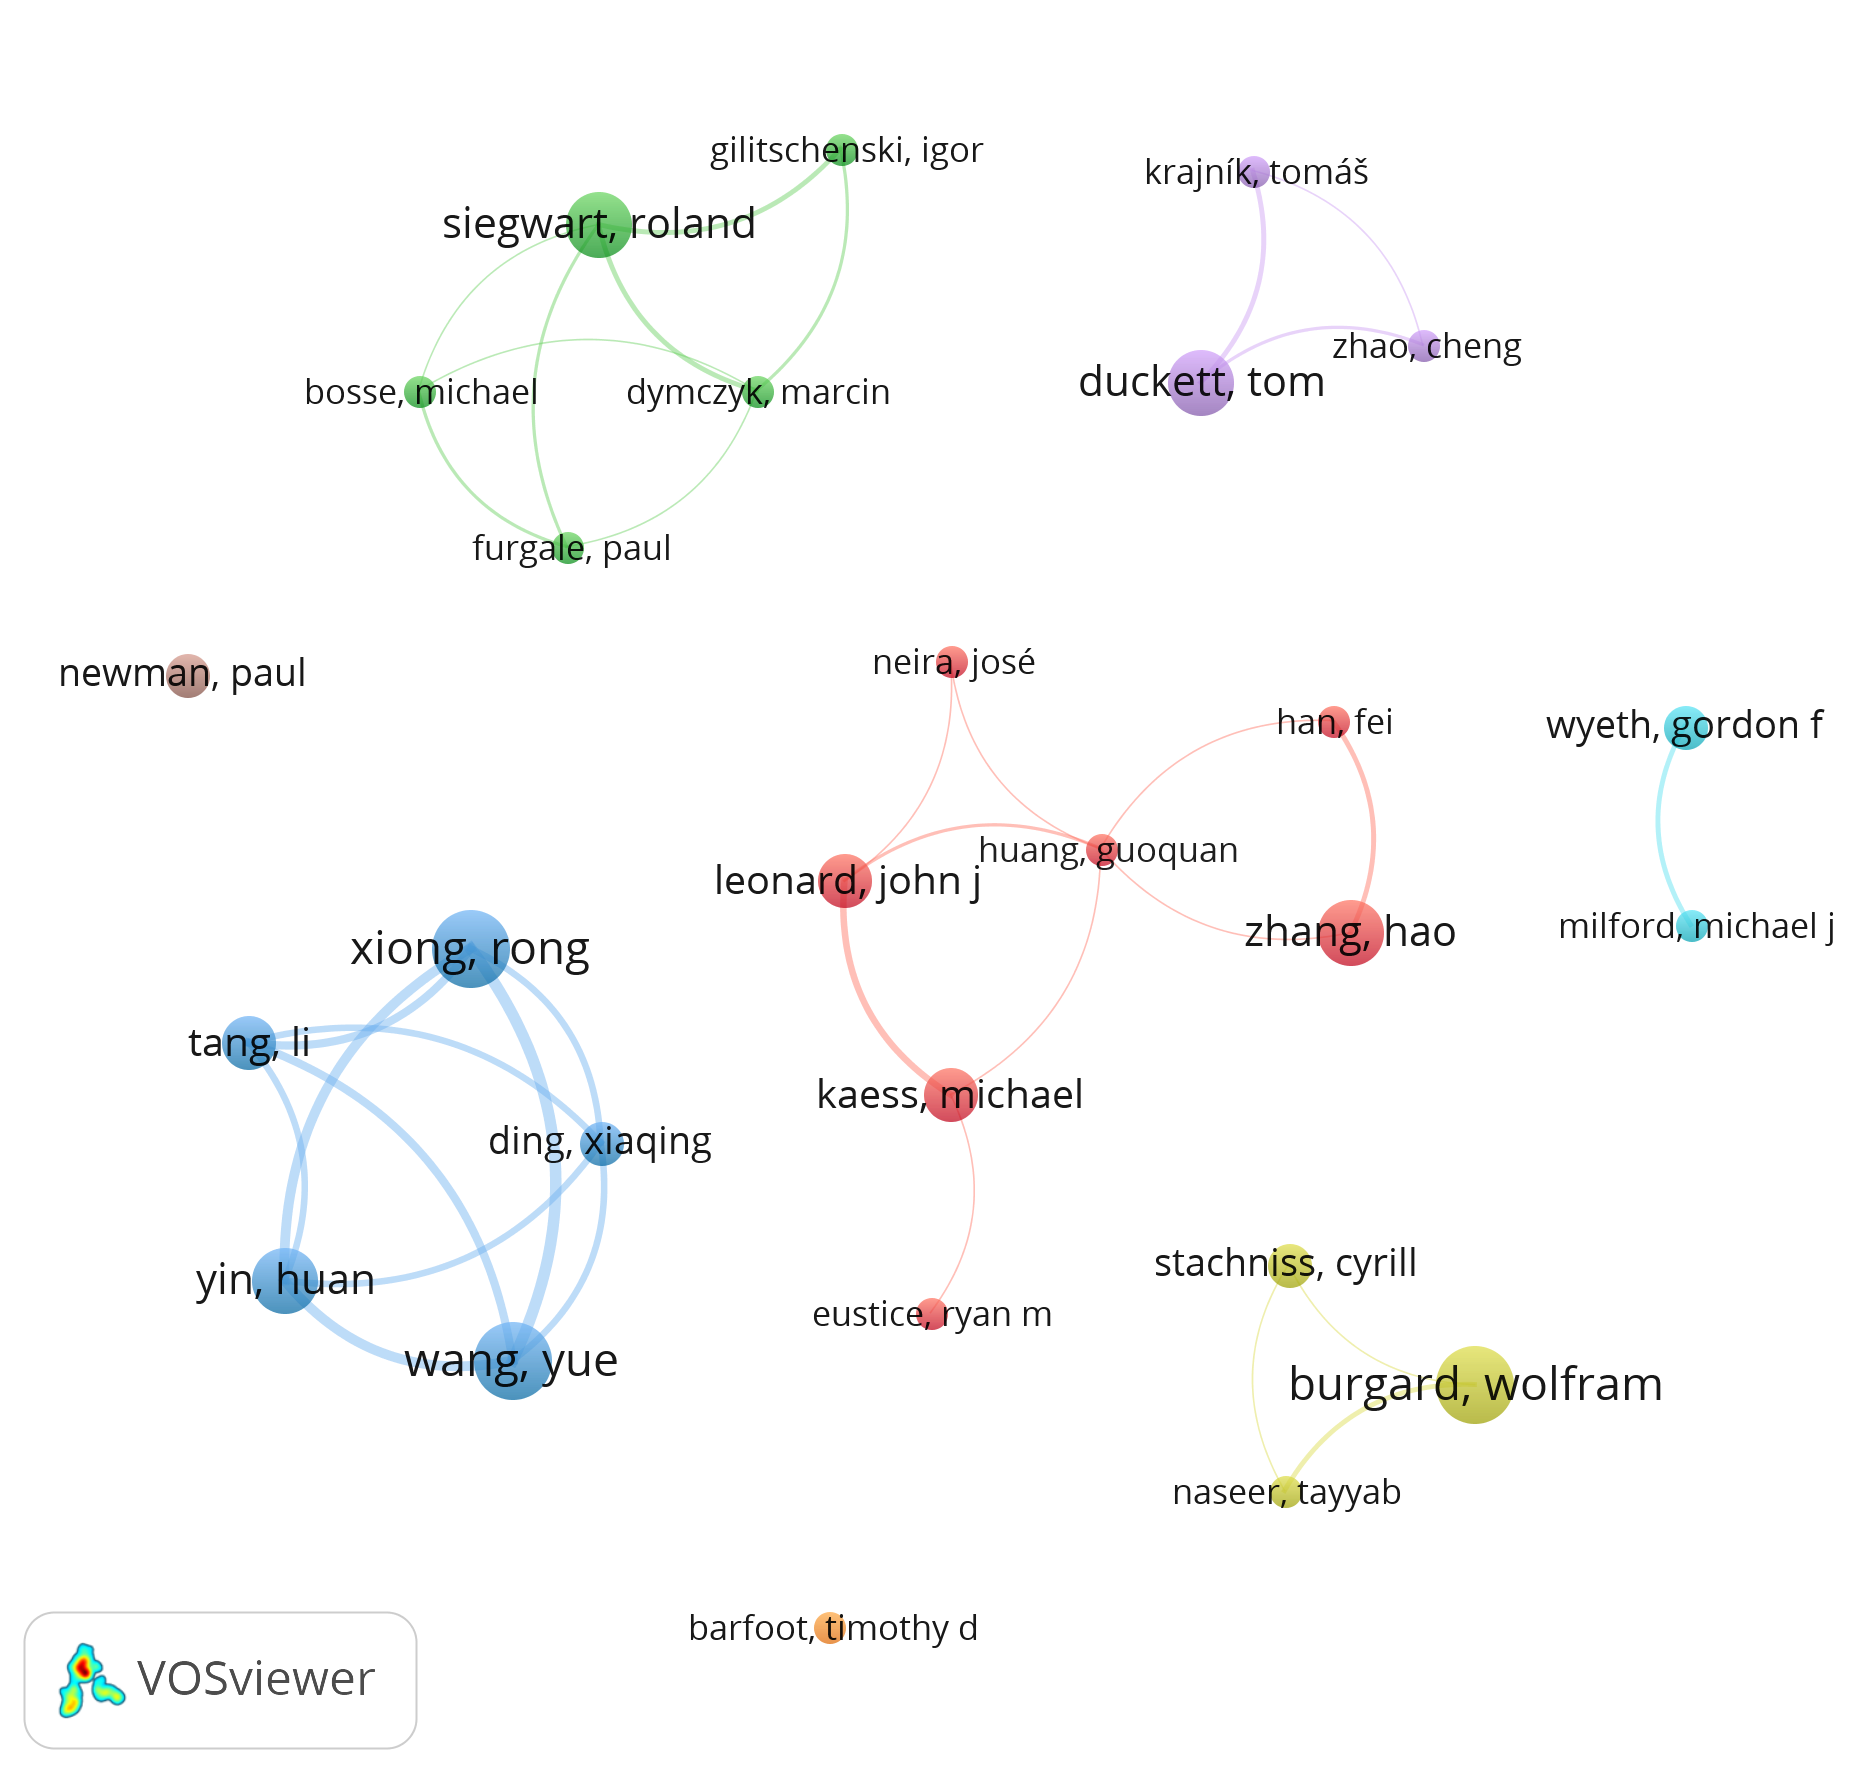
\includegraphics[width=\columnwidth]{figures/authors.png}
  \caption{Co-authorship analysis on the 142 included records generated by VOSviewer. Parameters used for generating the co-occurrence network: minimum number of occurrences = 3, attraction = 4, repulsion = -2, scale = 1.49, circles size variation = 1.0, lines size validation = 1.0.}
  \label{fig:overview:authors}
\end{figure}

Analyzing Figure~\ref{fig:overview:authors}, the co-authorship network presents 8 clusters. These clusters are separated from each other, i.e., no link exists between authors from different clusters. However, this separation does not mean that there is not any co-authorship between authors from different clusters only indicating that for a minimum of 3 co-authored documents there is not a connection between the authors of these 8 clusters. Even so, the graph presented in Figure~\ref{fig:overview:authors} allows the identification of the most relevant research networks in terms of number of co-authored documents and in the context of long-term localization and mapping, considering the 142 records included in this review. As a results, the following enumeration presents the authors that belong to each cluster in the format of author (number of co-authored documents):

\begin{enumerate}\setlength\itemsep{-0.5em}
\item Rong Xiong \orcid{0000-0001-9318-9014}\textsuperscript{,}\scholar{1hI9bqUAAAAJ} (7),
      Yue Wang \orcid{0000-0002-0981-935X}\textsuperscript{,}\scholar{N543LSoAAAAJ} (7),
      Huan Yin \orcid{0000-0002-0872-8202}\textsuperscript{,}\scholar{1fNc3vUAAAAJ} (6),
      Li Tang \orcid{0000-0003-2590-6872} (5), and
      Xiaqing Ding \orcid{0000-0001-7802-0130}\textsuperscript{,}\scholar{6u5OHUcAAAAJ} (4);
\item Hao Zhang \scholar{Ug2VxyUAAAAJ} (6),
      John J. Leonard \orcid{0000-0002-8863-6550}\textsuperscript{,}\scholar{WPe7vWwAAAAJ} (5),
      Michael Kaess \scholar{27eupmsAAAAJ} (5),
      Fei Han \orcid{0000-0002-8619-3987} (3),
      Guoquan Huang \scholar{trMUyZIAAAAJ} (3),
      José Neira \orcid{0000-0003-0668-977X}\textsuperscript{,}\scholar{scoMbR8AAAAJ} (3), and
      Ryan M. Eustice \orcid{0000-0002-9989-4942}\textsuperscript{,}\scholar{WroYmiAAAAAJ} (3);
\item Wolfram Burgard \orcid{0000-0002-5680-6500}\textsuperscript{,}\scholar{zj6FavAAAAAJ} (7),
      Cyrill Stachniss \orcid{0000-0003-1173-6972}\textsuperscript{,}\scholar{8vib2lAAAAAJ} (4), and
      Tayyab Naseer \orcid{0000-0002-3350-3005}\textsuperscript{,}\scholar{1FePZqEAAAAJ} (3);
\item Roland Siegwart \orcid{0000-0002-2760-7983}\textsuperscript{,}\scholar{MDIyLnwAAAAJ} (6),
      Igor Gilitschenski \orcid{0000-0001-6426-365X}\textsuperscript{,}\scholar{Nuw1Y4oAAAAJ} (3),
      Marcin Dymczyk \orcid{0000-0003-3667-8764}\textsuperscript{,}\scholar{XYHy7U8AAAAJ} (3),
      Michael Bosse \scholar{eopb1VgAAAAJ} (3), and
      Paul Furgale \orcid{0000-0002-7367-1046}\textsuperscript{,}\scholar{RNDtSG8AAAAJ} (3);
\item Tom Duckett \orcid{0000-0003-2971-7905}\textsuperscript{,}\scholar{et1GU2EAAAAJ} (6),
      Cheng Zhao \orcid{0000-0001-8502-3233}\textsuperscript{,}\scholar{EAC-8m0AAAAJ} (3), and
      Tomáš Krajník \orcid{0000-0002-4408-7916}\textsuperscript{,}\scholar{Qv3nqgsAAAAJ} (3);
\item Gordon F. Wyeth \orcid{0000-0002-4996-3612}\textsuperscript{,}\scholar{yfXZfXEAAAAJ} (4) and
      Michael J. Milford \orcid{0000-0002-5162-1793}\textsuperscript{,}\scholar{TDSmCKgAAAAJ} (3);
\item Paul Newman \scholar{BtO5fTUAAAAJ} (4);
\item Timothy D. Barfoot \orcid{0000-0003-3899-631X}\textsuperscript{,}\scholar{N_vPIhoAAAAJ} (3).
\end{enumerate}

When analyzing the affiliations of the authors mentioned previously at the time of publication, all authors of the first cluster belonged to the State Key Laboratory of Industrial Control and Technology (SKLICT) and the Institute of Cyber-Systems and Control at Zhejiang University in China. Even though Huan Yin, Yue Wang, Xiaqing Ding, Li Tang, and Rong Xiong mention their affiliation to the Joint Centre for Robotics Research between Zhejiang University, China, and the University of Technology Sydney, Sydney, in the work \cite{yin-et-al:2020:2905046}, this specific affiliation only appeared in this article. The total link strength (sum of all links weights) of each of the authors in that cluster is higher than 16, meaning a high co-authorship between them. Indeed, all five authors have links between all of them.
Similar to the first cluster, the third, fourth, fifth, and sixth clusters have common affiliations within each one: the Autonomous Intelligent Systems at the University of Freiburg in Germany, the Autonomous Systems Lab (ASL) at ETH Zürich in Switzerland, the Lincoln Centre for Autonomous Systems (LCAS) at the University of Lincoln in UK, and the School of Electrical Engineering and Computer Science at Queensland University of Technology (QUT) in Australia, respectively.
However, the interlinking between the authors is not as strong as in the first cluster, as shown in Figure~\ref{fig:overview:authors} by the authors of these clusters not being connected between all the ones within each cluster. Even so, the common affiliation shows there is considerable interest by these research units in the long-term localization and mapping topic.

The affiliation analysis in the second cluster is more complex given that there was no affiliation common to all authors at the time of the records' publication. Instead, the following affiliations were found: Fei Han and Hao Zhang with the Department of Computer Science at Colorado School of Mines in the USA, Guoquan Huang with the Department of Mechanical Engineering at the University of Delaware in the USA, John J. Leonard and Michael Kaess with the Computer Science and Artificial Intelligence Laboratory (CSAIL) at the Massachusetts Institute of Technology (MIT) in the USA, Ryan M. Eustice with the Perceptual Robotics Laboratory (PeRL) at the University of Michigan in the USA, and José Neira with the Instituto Universitario de Investigación en Ingeniería de Aragón (I3A) at the Universidad de Zaragoza in Spain.
Although there are 5 different affiliations to which the 7 authors stated in the respective records, 4 of the research institutions noted for the second cluster are in the USA, indicating a possible reason for facilitating the linkage between these authors from different research units.

In terms of the clusters composed by single authors, the affiliations of Paul Newman and Timothy D. Barfoot are the Oxford Robotics Institute at the University of Oxford in UK and the Autonomous Space Robotics Laboratory (ASRL) at the University of Toronto Institute for Aerospace Studies (UTIAS) in Canada, respectively. Even though these two authors are not linked with any others in the network, the co-authorship analysis indicates that they have an interest in long-term localization and mapping. This interest is shown by their number of co-authored records: 4 and 3 by Paul Newman and Timothy D. Barfoot, respectively.

As for the number of co-authored publications, considering the 142 included records, the authors that appeared to have more research on the review's topic are Rong Xiong, Yue Wang, and Wolfram Burgard, given the 7 co-authored publications of each one. However, Rong Xiong and Yue Wang have co-authored the 7 documents attributed to each of them. This relation and similar ones can biase the analysis of which authors are having more impact in the review's topic.
The clustering shown in Figure~\ref{fig:overview:authors} allows a more unbiased analysis relative to the co-authorship links between authors. Thus, based on the clustering and which author from each cluster has the most co-authored publications, the most influential authors in long-term localization and mapping are the following ones: Rong Xiong (or Yue Wang), Hao Zhang, Wolfram Burgard, Roland Siegwart, Tom Duckett, Gordon F. Wyeth, Paul Newman, and Timothy D. Barfoot.

\subsection{Year of publication}
\label{sec:overview:year}

The relevance of the long-term localization and mapping topic can be evaluated by the evolution of the number of publications. Figure~\ref{fig:overview:year} presents this evolution from the earliest year of publication of the included records to the year at the time of writing this article. The latter has its respective data dashed to indicate that the last year is not completed at the time of writing. Analyzing Figure~\ref{fig:overview:year}, this review's topic seems to have gain relevance in 2009 with 6 works, compared to only one publication in 2007 and another in 2002 in the previous years to 2009. From that year onwards, the graph has an almost linear tendency reaching a maximum of 23 records in 2021, while already having 8 publications in 2022 until May 17, 2022. This tendency shows that long-term localization and mapping is gaining interest throughout the years and, consequently, supports the importance and relevance of this review for the scientific community.

\begin{figure}[!h]
  \centering
  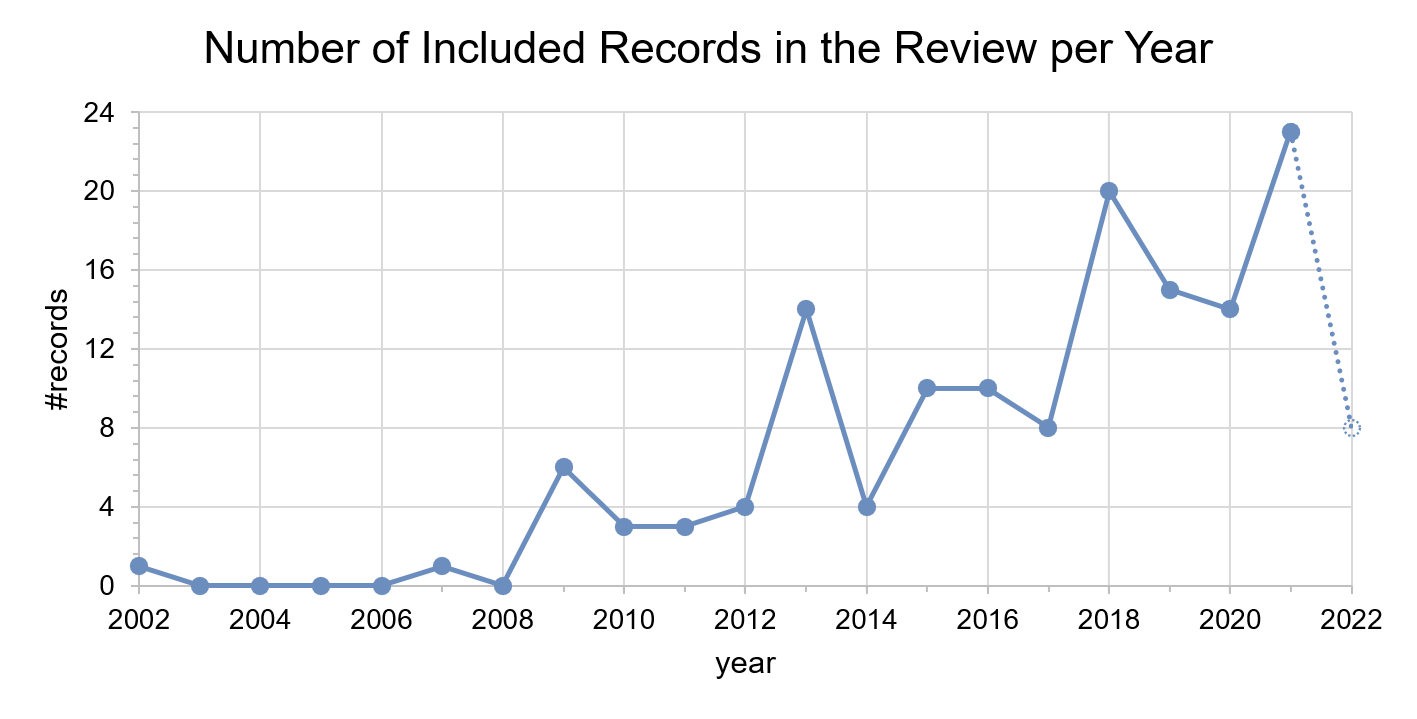
\includegraphics[width=\columnwidth]{figures/year.png}
  \caption{Evolution of published records per year considering the 142 included records in this review.}
  \label{fig:overview:year}
\end{figure}

\subsection{Publication venue}
\label{sec:overview:publication}

Finally, the last overview of the 142 included records in the review is relative to the publication venue. Table~\ref{tab:overview:publication} presents the venues with more than 1 publication, separating the journals and conferences in two different tables (Tables~\ref{tab:overview:publication:journal} and \ref{tab:overview:publication:conference}, respectively).
The columns $\mu$ present the average year of publication of the records associated to a certain venue, while $\text{max}$ columns display the publishing recency by the year of the most recent publication in the venue. For comparing to the average value ($\mu$), the third column ($\sigma$) of each table presents the standard deviation based on the publication year data.
The last column state the number of records published in the venue from the 142 records included in the review for discussion.

\begin{table}[!h]
  \centering
  \caption{Publication venues of the included records in this review with more than one record published in the venue: (a) journals; (b) conferences. Legend: $\mu$ -- average year of publication, $\sigma$ -- standard deviation of the publication year, $\text{max}$ -- maximum year of publication, \# -- number of records published at a certain venue.}
  \label{tab:overview:publication}
  \subfloat[][]{%
  \begin{tabular}{p{0.55\columnwidth}cccc}
\hline
                 & \multicolumn{3}{c}{\textbf{Year}} & \\
\cline{2-4}
\textbf{Journal} & $\mu$ & $\sigma$ & $\text{max}$ & \textbf{\#}\\
\hline
Robotics and Autonomous Systems & 2016 & 3.9 & 2021 & 13\\
IEEE Robotics and Automation Letters & 2019 & 1.7 & 2022 & 12\\
International Journal of Robotics Research & 2014 & 3.2 & 2022 & 11\\
Journal of Field Robotics & 2017 & 3.5 & 2022 & 8\\
Autonomous Robots & 2017 & 2.2 & 2020 & 7\\
IEEE Transactions on Intelligent Transportation Systems & 2021 & 0.8 & 2022 & 4\\
Sensors & 2019 & 0.8 & 2020 & 4\\
IEEE Transactions on Robotics & 2017 & 3.1 & 2022 & 4\\
IEEE Sensors Journal & 2020 & 1.5 & 2021 & 2\\
International Journal of Advanced Robotic Systems & 2020 & 1.5 & 2021 & 2\\
\hline
  \end{tabular}\label{tab:overview:publication:journal}%
  }
  \linebreak
  \subfloat[][]{%
  \begin{tabular}{p{0.55\columnwidth}cccc}
\hline
                    & \multicolumn{3}{c}{\textbf{Year}} & \\
\cline{2-4}
\textbf{Conference} & $\mu$ & $\sigma$ & $\text{max}$ & \textbf{\#}\\
\hline
IEEE International Conference on Robotics and Automation (ICRA) & 2016 & 3.9 & 2021 & 22\\
IEEE/RSJ International Conference on Intelligent Robots and Systems (IROS) & 2017 & 3.6 & 2021 & 17\\
IEEE International Conference on Robotics and Biomimetics (ROBIO) & 2019 & 2.1 & 2021 & 3\\
IEEE International Intelligent Transportation Systems Conference (ITSC) & 2018 & 2.4 & 2021 & 3\\
European Conference on Mobile Robots (ECMR) & 2014 & 0.9 & 2015 & 3\\
IEEE Intelligent Vehicles Symposium (IV) & 2019 & 0.5 & 2019 & 2\\
International Conference on 3D Vision (3DV) & 2018 & 1.5 & 2019 & 2\\
International Conference on Advanced Robotics (ICAR) & 2011 & 2.0 & 2013 & 2\\
\hline
  \end{tabular}\label{tab:overview:publication:conference}%
  }
\end{table}

In terms of journals, the Robotics and Autonomous Systems, IEEE Robotics and Automation Letters, and the International Journal of Robotics stand out with more than 10 publications. Also, these journals have a high standard deviation (greater than 1.5), indicating that the publications spread out throughout the years.
In the case of the IEEE Robotics and Automation Letters, these results gain more relevance indicating a recent trend on publishing on this journal, considering that its creation was only on 2015\footnote{\url{https://www.ieee-ras.org/publications/ra-l}}.
With more than 5 publications, the Journal of Field Robotics and the Autonomous Robots have recent average of publication (2017) with a high standard deviation (greater than 2.0), similarly indicating that authors have been publishing in these two journals along the years.
In contrast, the IEEE Transactions on Intelligent Transportation Systems and Sensors journals have a standard deviation lower than 1 year, with an average publication year of at least 2019. The recency of publication on these two journals with a very low deviation suggests a recent interest of the authors to publish in these two journals works related to long-term localization and mapping.

As for conferences, the data in Table~\ref{tab:overview:publication:conference} shows a high discrepancy in the number of publications related to this review's topic in ICRA and IROS compared to the other venues. Indeed, all the other conferences have only a maximum of 3 records published in them, compared to 22 and 17 papers in ICRA and IROS, respectively. When considering that 60 of the 142 included records are published in conferences, ICRA and IROS with a total of 39 published works related to this review's topic represent 65\% of works published in conferences and 27.5\% of all included records. This result expresses the high relevance of ICRA and IROS in the topic of long-term localization and mapping.


\section{Discussion}
\label{sec:discussion}

The main goal of this review is to synthesize methodologies focused on long-term localization and mapping. Therefore, the discussion first analyzes the techniques proposed in the 142 included works for the five categories of DE1 (see Section~\ref{sec:methodology:data}). Section~\ref{sec:discussion:appearance} discusses methodologies related to dealing with the varying appearance of environments for localization and place recognition. Section~\ref{sec:discussion:dynamics} analyzes works focused on modeling the environment dynamics or identifying dynamic objects within the environment. Section~\ref{sec:discussion:sparsity} focuses on approaches for removing redundant data from the map or identifying novelty data to keep the map size constrained to the environment size. Section~\ref{sec:discussion:multisession} discusses how methods handle multi-session in terms of mapping. Section~\ref{sec:discussion:computational} reviews works related to computation concerns over long-term localization and mapping, in addition to the ones relative to map sparsification discussed in Section~\ref{sec:discussion:sparsity}. However, the discussion should also focus on how the included works evaluated their results in long-term operations. Thus, Section~\ref{sec:discussion:experiments} analyzes the experimental data and datasets used in the experiments, and Section~\ref{sec:discussion:metrics} presents the evaluation metrics used for evaluating the proposed methodologies.





\subsection{Appearance variance}
\label{sec:discussion:appearance}

Next, the discussion focuses on included works categorized in DE1 as appearance. The different methodologies found in these works deal with variable lighting changes, perspective or viewpoint variance, moving elements in the scene, different weather conditions, or changes caused by the year's seasons.
In order to improve the discussion, the analysis of the proposed techniques related with appearance invariance is organized into the following topics: experience maps for treating different appearances as multiples experiences, handcrafted features, features extracted using Convolutional Neural Networks (CNN), assessment of feature stability, multi-modal features, leverage of temporal coherence by image sequence matching, and a discussion of the different sensors modalities used in the included works for appearance invariance.



\subsubsection{Experience maps}
\label{sec:discussion:appearance:exp-maps}

One way to deal with the appearance variance of environments is by treating different conditions as multiple experiences.
The biologically inspired RatSLAM~\parencite{ball-et-al:2013:9} introduces the experience map as a semi-metric topological map, where each experience is a view of the environment at a certain position and wheel odometry provides the relative pose for the links. New experiences are created when none of the previous ones saved in the map are sufficiently similar in appearance to the current scene.
\cite{glover-et-al:2010:5509547} combines the mapping of RatSLAM with the place recognition of FAB-MAP~\parencite{discussion:fab-map}. The latter improves the loop closure detection of the original RatSLAM due to FAB-MAP having light invariant characteristics for data association by learning a generative model for the Bag of Words (BoW) model~\parencite{discussion:bow}.
Both RatSLAM and the hybrid RatSLAM+FAB-MAP systems uses visual data to retrieve information from the environment.
Although \cite{martini-et-al:2020:s20216002} uses also experience-based mapping, the main sensor is a radar, where an experience is represented by a point cloud from the sensor and the point descriptors retrieved from it. Radar is known for being less affected by environment changes such as different illumination or weather conditions compared to vision sensors~\parencite{hong-et-al:2022:02783649221080483}.

The concept of adding the environment changes to the map identified by the degradation in localization is also employed by \cite{konolige-bowman:2009:5354121} and \cite{tang-et-al:2019:7}.
The former implements a keyframe SLAM system created from the Visual Odometry (VO) module, where each keyframe represents a view of the environment, while a place recognition module tries to match the current frame to similar views already in the map for loop closure.
The latter applies a similar idea to experience maps based on the 2D manifold assumption for locally smooth navigation. Even though the proposed topological local-metric framework encodes geometric information in the edges, the nodes do not require global pose, i.e., no restriction for global consistency. New nodes are trigered either from localization failure or after a certain length is traveled by the robot. The goal is to restrict the erroneous alignment computed from odometry locally.

Instead of considering an experience as a location or a view of the current scene, \cite{churchill-newman:2013:0278364913499193} defines it as a whole sequence of the saved poses and related features directly obtained from VO. In this case, the topological mapping links experiences not geometrically but instead if two experiences observe the same space. However, the method does not implement a specific place recognition module for loop closure, assuming that the robot will subsequently return to a place that can have successful localization.
\cite{gadd-newman:2016:7759843} builds on the work of \cite{churchill-newman:2013:0278364913499193} for multi-robot systems. This method adds FAB-MAP for place recognition in the existing map maintained by a centralized versioning framework. The selection of the most relevant experiences by the centralized framework for localizing multiple agents in the system assumes that appearance change is only driven by the passage of day time.

Another example of experience maps is Visual Teach \& Repeat systems using spatial-temporal pose graphs, as implemented in \cite{mactavish-et-al:2018:21838} and \cite{zhang-et-al:2018:8460674}.
Similar to \cite{churchill-newman:2013:0278364913499193}, an experience is the output of the VO module defining the appearance of a scene throughout a path. In the teaching phase, the robot is teleoperated by humans creating privileged experiences in the graph.
Autonomous experiences are the ones relative to the repetition phase. These experiences are linked either temporally or spatially if they are sequential in time or related metrically by multi-experience matching, respectively.
Unlike \cite{churchill-newman:2013:0278364913499193}, new experiences have a known metric pose relative to the others in the pose graph.

In general, experience-based navigation methods try to generate new experiences if the environment changes, expecting that at a certain point in time the robot will be able to localize itself relative to previous experiences, not requiring new ones to be added to the map.
However, these approaches are not scalable in the long-term time frame nor to deal with dynamic elements, even using central servers as in \cite{gadd-newman:2016:7759843} with more computational resources than the robots.
Pruning algorithms would be required to remove redundant or outdated information, as in \cite{konolige-bowman:2009:5354121} or \cite{tang-et-al:2019:7}.
Also, other methods should be employed to deal not only with long-term appearance changes (weather conditions or seasonal changes) but also with dynamic elements in the scene.



\subsubsection{Illumination transformations}
\label{sec:discussion:appearance:illumination}

As a preprocessing step, illumination invariant transformations can be applied to color images for increasing the robustness of visual localization to changing lighting conditions and shadows.
One example is the illumination invariant space that combines the log-responses of the 3 color channels into an one-dimensional space with a weighting parameter conditioned by the peak spectral responses of each channel, usually available in the camera specifications. This one-dimensional space is only dependent on the sensor and elements in the scene, while being independent of the intensities and colors.
Both works of \cite{arroyo-et-al:2018:7} and \cite{yang-et-al:2021:12054} uses this transformation for preprocessing the color images into grayscale ones demonstrating the robustness of the illumination invariant space when lighting changes appear.

An alternative to using predefined illumination invariant transformations is to learn them.
\cite{clement-et-al:2020:2967659} learns a nonlinear transformation mapping function from the RGB color space to grayscale also combining the three-channel log-responses, but relaxing the constraints of the one-dimensional space due to the original weighting parameter used in \cite{arroyo-et-al:2018:7} and \cite{yang-et-al:2021:12054}. Instead of using the same parameters independently of the image content, \cite{clement-et-al:2020:2967659} trains an encoder to predict the optimal transformation weighting parameters of the three-channel log-responses.
The objective function chosen for maximization is based on the number of inlier feature matches from a vision localization pipeline.
The learned nonlinear RGB to grayscale transformation helped achieving a full-day cycle using a single mapping experience and the applying the optimized transformation to the color images.

Even though the Gamma correction does not transform an image to an invariant color space, this transformation can be used to strengthen low-illumination changes. \cite{sun-et-al:2021:9635886} uses the Gamma transform to synthesize low-illumination night-time images from daytime ones. Applying the transformation in the HSV (Hue, Saturation, Value) space, the gamma parameter adjusts the value channel without distorting the colors. Then, the synthesized images are used for training the DarkPoint descriptor proposed by \cite{sun-et-al:2021:9635886} to improve day-to-night matching.



\subsubsection{Handcrafted features}
\label{sec:discussion:appearance:handcrafted}

Many localization and mapping algorithms rely on detection and extraction of features. The designation of handcrafted features refers to properties derived from the sensors data as a two-step process: a keypoint detector to locate the features and their characterization by computing a descriptor capable of distinguishing each feature from the others~\parencite{discussion:handcrafted-features}.
Algorithms for long-term localization and mapping using handcrafted feature should be robust to changing conditions such as illumination, appearance, weather and seasonal changes.


\paragraph{Visual features}

A way to improve long-term feature-based visual localization is to enhance the descriptiveness of visual feature descriptors and their long-term stability.
\cite{kawewong-et-al:2013:826410} defines the Position Invariant Robust Features (PIRF). In a sliding window framework, PIRF tracks the motion of local features such as Scale-Invariant Feature Transform (SIFT) or Speeded Up Robust Features (SURF) selecting the stable ones.
Using an incremental tree-like PIRF (with inverted index as in BoW) dictionary, the method has shown robustness to viewpoint variance and unstable features. Also, PIRF-based localization improved the recall over FAB-MAP in the experiments.

Moreover, Histogram of Oriented Gradients (HOG) features have been used in different works to improve robustness to appearance variance, given that HOG descriptors capture local gradient information robust to seasonal changes \parencite{naseer-et-al:2015:7324181}.
\cite{li-et-al:2015:7139706} computes local HOG descriptors from visually-salient image patch features in an underwater environment. Using a trained Support-Vector Machine (SVM) to classify the matching between corresponding patches, the method achieved approximately 80\% accuracy with dramatic appearance changes.
Although \cite{naseer-et-al:2015:7324181} computes HOG descriptors from each cell of a partitioned image, a global descriptor for the whole image joins all the cell ones. The global descriptor proved to be robust to foliage color changes, occlusions, and seasonal changes.
\cite{vysotska-et-al:2015:7139576} uses the same global HOG descriptor as in \cite{naseer-et-al:2015:7324181}, but applied to image sequence matching requiring a rough global pose estimation for the images (e.g., GPS) for efficient matching.

Local Difference Binary (LDB) features also include gradient comparisons. These features are used in the Able for Binary-appearance Loop-closure Evaluation (ABLE) \parencite{arroyo-et-al:2018:7} approach to achieve higher descriptiveness power for appearance invariance.
ABLE outperformed FAB-MAP in terms of precision-recall evaluation metrics. An advantage of using binary features such as LDB is the possibility of using the Hamming distance to compute descriptor similarity, improving the computational efficiency of this process over cosine similarity or Euclidean distance.

Another work from the included records focused on improving the long-term performance of handcrafted visual features is from \cite{karaoguz-bozma:2016:4}. Their approach uses bubble descriptors for preserving the relative $S^2$ geometry of visual features, being rotationally invariant. The experimental results demonstrated improvements on viewpoint and illumination invariance of bubble features-based localization.

Instead of preserving the long-term appearance-invariance of visual descriptors, \cite{neubert-et-al:2015:005} introduces the SuperPixel-based Appearance Change Prediction (SP-ACP) to predict extreme appearance changes across seasons.
SP-ACP extracts descriptors (combination of color histogram in Lab color space with upright SURF descriptor) from the image superpixels and clusters the descriptors into seasonal-specific vocabularies using hierarchical k-means.
With training images with pixel-accurate alignment between images, the known pixel association creates a translation dictionary between seasons to synthesize a predicted image for cross-season place recognition.
SP-ACP was able to improve cross-season place recognition performance compared to not comparing with the predicted image, although the method has the limitation of requiring pixel-wise alignment in training.

The work of \cite{griffith-pradalier:2017:21664} considers GPS and compass data in addition to visual data. \cite{griffith-pradalier:2017:21664} builds on SIFT Flow to find dense correspondences among images for survey registration in long-term lakeshore monitoring. SIFT Flow combines the precision of point-based feature matching with the robustness of whole-image matching, while the GPS, the feature tracks from a visual SLAM, and the compass measurements bias the image registration. The proposed method was able to match images from different surveys separated by several months with dramatic changes relative to lighting, occlusions, seasonal changes, and even the sun glare.

Even though \cite{cao-et-al:2018:2815956} and \cite{cao-et-al:2021:2962416} require a 2D or a 3D laser for place recognition and not a visual sensor, these methods use 2D image representations of a point cloud to extract visual handcrafted features.
\cite{cao-et-al:2018:2815956} transforms the 3D point clouds of a 3D laser into 2D images using the bearing angle 2D representation (image according to the relative position among adjacent laser points, without projecting the point cloud onto a certain surface). Using a BoW approach with the dictionary learned using ORB features, the query image is matched to the database ones, while performing geometric verification by reprojecting the ORB features into the 3D coordinate frame. One main advantage of using LiDAR in the experiments was its less sensitivity to lighting conditions relative to visual sensors while not being incapacitated in dark environments. The proposed method outperformed M2DP~\parencite{discussion:m2dp} -- global descriptor for point clouds --, given that M2DP could not deal in situations where the point clouds distributions were centralized and similar to each other.
As for \cite{cao-et-al:2021:2962416}, the proposed method accepts also 2D laser data by accumulating a sequence of scans. The 2D representation used differs from \cite{cao-et-al:2018:2815956} by projecting the point cloud into cylindrical coordinates and using the centroid of the point cloud to ensure viewpoint invariance.
Using Gabor filters to detect and describe the contours of the images, \cite{cao-et-al:2021:2962416} generates Binary Robust Independent Elementary Features (BRIEF) descriptors for matching images using a nearest neighbors search. In addition to showing the seasonal appearance variance in laser data (e.g., different foliage in the scene), the proposed methodology outperforms SeqSLAM~\parencite{discussion:seqslam} (sequential place recognition) and PointNetVLAD~\parencite{discussion:pointnetvlad} (CNN-based place recognition for 3D point clouds) on precision-recall.

In terms of visual features from radar data, \cite{hong-et-al:2022:02783649221080483} extracts visual features used for tracking using a blob detector based on a Hessian matrix. These features are extracted from a 2D cartesian image transformed from the polar image representation of radar, while also compensating the distortion from the vehicle's motion.
As for loop closure detection, the peaks in intensity from the polar radar image are evaluated to remove noise of areas without a real object due to speckle noise. Then, the processed polar image is transformed into a point cloud and the M2DP descriptor adapted to 2D point clouds is used to detect loop closure.
The proposed methodology improved the radar odometry tracking, while also outperforming ORB-SLAM2~\parencite{discussion:orb-slam2}.


\paragraph{Environment structure features}

The structure of the environment defined by its geometry is more robust to appearance variance than the appearance itself. Common structure features extracted from sensors data are line and edge features.
\cite{biswas-veloso:2013:0278364913503892} extracts 2D line segments corresponding to the walls from depth and 2D laser sensors. The line segment-based localization had a low failure rate on an over-a-year long-term indoor deployment even in areas with movable objects, due to the long-term stability of the line segment features.
\cite{nuske-et-al:2009:20306} extracts 3D edge features of the scenes using a monocular camera to get the edges of the buildings in the environment, while employing an exposure control to maximize the strength of edges corresponding to the mapped ones. The proposed method was able to successfully track the edges of the buildings along an all-day outdoor experiment.
Instead of using the walls of the buildings, \cite{an-et-al:2016:0} formulates a visual node descriptor based on ceiling salient edge points. Even though the method achieved good results in lighting changing conditions, the method's performance decreases using low and inclined ceilings, due to the image perspective effect that may lead to matching failure in the implemented Iterative Closest Point (ICP) framework.

Furthermore, \cite{meng-et-al:2021:3062647} extracts edge and planar features by evaluating the large and small values of the local surface smoothness over the points of a 3D laser, respectively. ICP estimates the laser odometry while the histogram cross-correlation of the Normal Distribution Transform (NDT) that computes local probability density functions of the surface smoothness identifies the loop closures.
The proposed methods outperformed an ICP-based SLAM approach on Absolute Trajectory Error (ATE) in the experiments.
As for \cite{bosse-zlot:2009:009}, 2D point clouds segmented into connected components are clustered at regions of high curvature to get high curvature keypoints from multiple scans.
The proposed descriptor based on the moment grid improves outdoor place recognition relative to SIFT or Hough transform peaks due to the moment grid descriptor includes higher order of moments relative to other descriptors.

Poles are structures also used for long-term localization.
\cite{schaefer-et-al:2021:103709} retrieves the 2D coordinates of poles registered with a 3D laser. Results demonstrated the ability of reliable long-term localization over more than one year.
In addition to poles, \cite{berrio-et-al:2019:8814289} extracts also corner features from the 3D laser point cloud, being able to localize over a 6 month experiment at different times of the day.

Another possible application of environment structure features found in the included works is in crop fields for agriculture.
\cite{chebrolu-et-al:2018:2849603} formulates an aerial image registration algorithm based on the positions of the crops and the gaps between them remaining the same over time. The method computes a vegetation mask by exploiting the Excess Green Index (ExG) of RGB images. Using the Hough transform to find lines between vegetation, the center of the crops are the peaks on vegetation histograms perpendicular to the rows.
The testing results demonstrated invariance of the registration algorithm to changing conditions caused by weather and crop growth over one month.



\subsubsection{Convolutional Neural Networks (CNN)}
\label{sec:discussion:appearance:cnn}

A more recent direction noted in the included works is the use of CNN.
The evolution of deep learning in computer vision led to researching how CNN could be used for generating feature representations robust to appearance variance, as an alternative to handcrafted features.
CNN-based features are known to offer more discriminate power compared to handcrafted features while being able to be more robust in challenging environments~\parencite{taisho-kanji:2016:7866383}.
The feature representations can be retrieved from the layers of CNN, with earlier ones usually extract low-level features such as edges or corners, while deeper layers extract high-level ones such as semantic structures~\parencite{chen-et-al:2018:2859916}.
In addition to using the CNN feature maps, the included works also used CNN for semantic segmentation to extract semantic information from sensor data and appearance-content disentanglement for generating appearance-invariant descriptors.


\paragraph{CNN feature maps}

One application of CNN features is for image place recognition as a classification task. Instead of comparing pairs or triplets of images, the place recognition is formulated as a classification problem~\parencite{chen-et-al:2018:2859916}.
In \cite{taisho-kanji:2016:7866383}, the layer fc6 (fully connected) of AlexNet extracts 4096-dimensional CNN features from box regions in the query image, then reduced to 128-dimensional features with Principal Component Analysis (PCA). Comparing these features to the ones extracted from the reference images in a cross-domain library (collected in different routes and seasons), \cite{taisho-kanji:2016:7866383} defines the query image as a set of nearest neighbor library features (similar to BoW) and employs the image-to-class distance with the Naive Bayes Nearest Neighbor (NBNN) method. The proposed PCA-NBNN descriptor outperformed BoW and FAB-MAP on a cross-season experiment in precision-recall metrics.
\cite{chen-et-al:2018:2859916} also formulates a classification task for place recognition, using a VGG16 network for generating local features, while adding a convolutional a fully-connected, and a softmax layer to learn the correct label output for classification. The proposed architecture outperformed FABMAP and SeqSLAM on seasonal changing conditions.

Place recognition can also be formulated as a coarse to fine image matching problem. An initial set of reference image candidates is obtained based on nearest neighbor distances of image-wise global descriptors~\parencite{xin-et-al:2017:8310121,camara-et-al:2020:9196967,liu-et-al:2021:9561126}, while local features are used for obtaining a more accurate estimation based on spatial matching~\parencite{xin-et-al:2017:8310121,camara-et-al:2020:9196967} or geometrical verification~\parencite{liu-et-al:2021:9561126}.
\cite{xin-et-al:2017:8310121} extracts both global and local features using a convolutional layer (conv3) of the AlexNet network, where local features are extracted from regions of the image with candidate regions sorted by the objectness score (improves viewpoint invariance).
Instead of using AlexNet, \cite{camara-et-al:2020:9196967} uses layers from VGG16 for feature extraction, specifically, conv5-2 and conv4-2 layers for global and local features, respectively.
As for \cite{liu-et-al:2021:9561126}, the MobileNetV2 network is selected for global feature extraction due to its computational efficiency. However, their work uses grid-based motion statistics with Oriented FAST and Rotated BRIEF (ORB) local features instead of CNN features.

Deep features can be combined with handcrafted features and preprocessing techniques to facilitate learning and further enhance their discriminative properties.
\cite{zhang-et-al:2022:3086822} uses the Key.Net network for keypoint generation, given that combines handcrafted and learned filters to detect keypoints at different scale levels, helping reduce the number of learnable parameters. Combined with HardNet for descriptor extraction, the method outperformed a BoW approach in viewpoint and illumination changing conditions.
\cite{yin-et-al:2020:2905046} proposes a handcrafted rotational invariant feature to be the input of a LocNet network for 3D laser-based place recognition. The proposed handcrafted feature reduced the complexity of the network and improved the efficiency on similarity evaluation.
As for preprocessing techniques to help in training, \cite{sun-et-al:2021:9635886} uses a the Gamma transform and other transformations (translation, scale, in-plane rotation, and symmetric perspective distortion) to generate day-nigh image pairs from daytime ones. These images are used for training the proposed visual descriptor DarkPoint on the keypoints generated by the SuperPoint keypoint detector. DarkPoint achieved approximately 1.7x more inliers during navigation than the original SuperPoint in day-night experiments.

Given that feature maps can extract different types of features depending on the deepness of the respective layers, \cite{zhu-et-al:2018:8500686} extracts features from three different layers (conv3-3, conv4-4, conv5-3) of a VGG16 network and concatenates these to form a global descriptor for an image. A cross-season experiment showed an increasing performance in precision-recall when the single layer gets deeper.
These results are conformal to ones obtained in \cite{yang-et-al:2021:12054}. The conv5-3 achieved higher accuracy than conv4-4 and conv3, indicating that the spatial information increases in deeper layers improving the place recognition. \cite{zhu-et-al:2018:8500686} also showed that fusing the three layers used in their work by concatenating them into a global descriptor improves even further the place recognition performance.
Moreover, \cite{yu-et-al:2019:8961714} chooses DenseNet for feature extraction due to this network reusing feature maps, i.e., connecting all layers with the same map sizes directly with each other. Then, \cite{yu-et-al:2019:8961714} uses the Weighted Vector of Locally Aggregated Descriptor (WVLAD) encoding for obtaining a global descriptor of the image. The proposed descriptor improved precision-recall over other architectures (VGG16, ResNet50) and to a BoW place recognition method.

The included works also focus on LiDAR and radar place recognition with CNN features. However, the raw point cloud data is not directly suitable for the CNN inputs. The most common solution is to project the point clouds onto the surface plane, the so-called Bird's-Eye View (BEV).
\cite{yin-et-al:2018:8593562} encodes directly the BEV of a LiDAR into a low dimensional global feature using a bidirectional Generative Adversarial Network (GAN). Using the extracted features within the SeqSLAM framework, the proposed method improved the precision-recall metrics over the original SeqSLAM in changing conditions.
Similarly, \cite{martini-et-al:2020:s20216002} extracts a global descriptor from the BEV using NetVLAD but with the point cloud from a radar sensor.
\cite{kim-et-al:2019:2897340} formulates the point cloud descriptor Scan Context Image (SCI), also known as ScanContext. The 3D point cloud is converted to a polar representation of BEV named Scan Context (SC) matrix, where each cell of the 2D matrix contains the maximum height of points around a scene. Using the jet colormap to transform the SC into the SCI as a three-channel image suitable for the CNN inputs, \cite{kim-et-al:2019:2897340} uses a LeNet network for feature extraction and place classification. The proposed architecture outperforms PointNetVLAD~\parencite{discussion:pointnetvlad} and the handcrafted point cloud feature M2DP in precision-recall.
Based on SCI~\parencite{kim-et-al:2019:2897340}, \cite{xu-et-al:2021:3060741} proposes the Differentiable Scan Context with Orientation (DiSCO) descriptor. This method distinguishes from SCI by applying the Fast Fourier Transformation (FFT) to convert the polar BEV representation to the frequency domain. Given that frequency spectrum is translation-invariant, DiSCO becomes rotation invariant. The results showed a superior performance to SCI and PointNetVLAD in changing conditions.
Similar to DiSCO~\parencite{xu-et-al:2021:3060741}, \cite{yin-et-al:2021:661199} also uses SCI and FFT for feature extraction of point clouds. The difference is the use of a shared U-Net architecture to extract features of LiDAR and radar data, training simultaneously the radar-to-radar, LiDAR-to-radar, and LiDAR-to-Lidar place recognition tasks. The proposed method had similar or improved performance in these three recognition tasks relative to SCI and DiSCO.
In addition to BEV, \cite{yin-et-al:2021:3061375} also uses the spherical view. Using two separated 2D CNN following the convolutional layers in VGG16 to encode local features, a VLAD layer extracts place features from each view (BEV and spherical). A tightly-coupled fusion network fuses the features of each view. The proposed FusionVLAD descriptor outperformed PointNetVLAD and M2DP on the recall metric in appearance variant conditions.

Lastly, a trend found in the included works to improve the discriminative power of CNN features is the use of triplets~\parencite{martini-et-al:2020:s20216002,liu-et-al:2021:9561126,piasco-et-al:2021:6,sun-et-al:2021:9635886,yin-et-al:2021:3061375,yin-et-al:2021:661199} in training.
A triplet consists in an anchor image, a positive corresponding match, and an unrelated negative example. Triplet loss tries to minimize the matching distance between positive pairs (anchor, positive) and maximize that between negative ones (anchor, negative)~\parencite{sun-et-al:2021:9635886}.
Additionally, \cite{piasco-et-al:2021:6} uses also depth information during training, given that depth maps and their geometric information remain more stable across time than visual ones. A CNN encoder aggregates local features to produce a global descriptor, while a decoder reconstructs the scene geometry from the features obtained by the encoder. Then, triplet loss during training uses the fusion of image and depth map descriptors. In the experiments, the depth map training supervision provided building shapes understanding while improving the performance compared to not using side information.


\paragraph{Semantic segmentation}

Instead of using the feature maps of CNN, the networks can also segment raw data to extract semantic information.
\cite{naseer-et-al:2017:7989305} uses the Fast-Net network for extracting saliency maps for stable structures. These structures considered in training are man-made ones such as buildings or signs that are presumable to be stable in long-term. Then, the salient maps boost the importance of features retrieved from a convolutional layer (conv3) for place recognition. The proposed method improved the precision-recall metrics compared to HOG and place recognition without boosting stable structures on a cross-season experiment.

The included works also use semantic features from pixel-wise labeling of image data.
\cite{qin-et-al:2020:9340939} modifies an U-Net for semantic feature detection specifically trained for parking lots. This network generates pixel-wise segmentation of lanes, parking lines, guide signs, speed bumps, free space, obstacles, and wall, used in both localization and feature mapping. In the experiments, the semantic features were robust to light changes, texture-less-regions, motion blur, and appearance change.
\cite{berrio-et-al:2021:3094485} also segments an image with pixel-wise labels, discriminating 12 classes: pole, building, road, vegetation, undrivable road, pedestrian, rider, sky, fence, vehicle, and unknown. Using the extrinsic parameters of the 3D laser--camera, the pixel-wise semantic information from the labeled images is transferred to the 3D point cloud. Then, pole and corner features are retrieved from the projected point cloud onto the horizontal plane based on the IMU data for localization and mapping. The long-term evaluation of the map corrections showed a decrease over time demonstrating the stability of these features in outdoor environments.
In addition to pixel-wise segmentation, \cite{singh-et-al:2021:9564866} connects the regions of each instance of the semantic classes to characterize them in terms of their centroid in 3D camera coordinates (using also depth information from a stereo camera) and connections to other regions. The proposed global semantic-geometric descriptor defines a location in terms of how the pairs of semantic entities are distributed in the scene. The proposed method obtained higher accuracy when compared to SeqSLAM, FAB-MAP, and a BoW-based place recognition methods in a highly dynamic outdoor experiment.

Similar to \cite{singh-et-al:2021:9564866}, graph embedding of semantic features also tries to integrate the relationships between features for improving the robustness of place recognition.
\cite{han-et-al:2018:2856274} proposes the Holism-And-Landmark Graph Embedding (HALGE) descriptor. In the training phase, an image is represented by its global HOG descriptor and semantic features (static or stable elements such as houses, traffic signs, trees).
A graph relates the training images from different domains and locations, where the nodes are images or the semantic classes, and the edges represent the presence of a semantic class in an image or if two images represent the same location.
Then, HALGE learns a projection matrix of each template database image from the graph to generate an appearance invariant feature from the original global HOG descriptor. The proposed method improved the performance over HOG, SURF, and color and AlexNet-based descriptors in changing conditions.
As for \cite{gao-zhang:2020:9196906}, the proposed method formulated the place recognition task into a graph matching problem. The graph represents each semantic feature (same classes as in \cite{singh-et-al:2021:9564866}) by its central position in the image coordinate frame, while the edges that relate the features represent theirs spatial distance and angular relations, and their appearance similarity (Euclidean distance of local HOG descriptors). Then, a graph optimization optimizes a correspondence matrix between the features in the query to the ones in the template images for obtaining the final matching scores, assuming a long-term worst-case scenario (maximizes the distance and angular similarities of features that have the least similar appearance).
The proposed method outperformed \cite{han-et-al:2018:3} and an HOG-based place recognition method on recall at higher precision in outdoor experiments with seasonal and weather changing conditions.

Semantic information can also be retrieved from other sensors such as LiDAR. \cite{wang-et-al:2021:9739599} uses the RangeNet++ network for inferring semantic labels of 3D point clouds from LiDAR data. Even though the network can label 10 different categories, the method only used the categories representative of pole-like objects (poles, tree trunks). The method achieved a higher localization accuracy than SCI~\parencite{kim-et-al:2019:2897340} in an outdoor experiment with moving elements and dense vegetation.


\paragraph{Appearance-content disentanglement}

A location has different representations due to weather or seasonal changing conditions in the long-term perspective, among other factors. In terms of image data, the information retrieved from these representations could be separated in terms of its contents and appearance. The included works studied this possibility by learning the appearance-content disentanglement for feature representation that assumes the decomposition of the images latent space into apperance and content spaces~\parencite{qin-et-al:2020:103561}.

\cite{oh-eoh:2021:app11198976} adopts a Variational AutoEncoders (VAE) architecture that uses an encoder to generate the appearance and content feature vectors, while a decoder reconstructs the original image from these vectors.
Instead of using a single encoder, \cite{qin-et-al:2020:103561} proposes the Feature Disentanglement Network (FDNet) consisting of independent content and an appearance encoders, a decoder, and also an appearance discriminator to ensure the vectors are unrelated. Even though the content feature vector demonstrated to invariant to seasonal changes, the method significantly reduced its performance on high viewpoint variance, where the content vector changed greatly while the appearance one did not changed at all. This results indicated that viewpoint change is considered to be content in the proposed algorithm.
With a similar architecture to \cite{qin-et-al:2020:103561}, \cite{tang-et-al:2021:17298814211037497} also considers a place domain discriminator to ensure that the content discriminator only contains the place information and not also its appearance, while also using data augmentation in training to increase robustness against viewpoint changes. In the experiments, all images generated from a zero-appearance feature vector looked similar, while their place information remains conserved indicating that the proposed method can disentangle the input image across appearance changes.

Even though \cite{hu-et-al:2022:1003907} does not extract appearance and content independent features from the images, the proposed architecture builds on the same assumption of appearance-content disentanglement that a content representation of a location is shared across multiple domains.
\cite{hu-et-al:2022:1003907} adopts a multi-domain image-to-image architecture that expands the CycleGAN architecture from two to multiple domains, with domain-specific encoder-decoder pairs and discriminators.
For obtaining a shared-latent feature across different domains, the descriptor is learned using the feature consistency loss for domain-invariance.
In the experiments, even though night-time images were not included in the training, the model was able to learn the content space of the places, while also outperforming FAB-MAP.



\subsubsection{Feature stability}

Although long-term handcrafted or CNN-based features intend to remain invariant to changing conditions of the environment, their long-term stability is not guaranteed to be the same for all detected features. In this context, \cite{dymczyk-et-al:2016:66} proposes a CNN architecture based on AlexNet for evaluating the feature stability for long-term visual localization. The network is trained using a set of labeled data pairs (image patch around the feature keypoint, label) or triplets (adds depth information), where the feature label is binary - stable or unstable - computed for training by assessing the number of the feature observations over multiple sessions. In the experiments of over 15 months and changing conditions, the proposed method outperformed random selection of features for localization in terms of f-score, while the addition of depth information improved the method's performance.

Other approaches in the included works define predictor functions for evaluating the feature stability.
\cite{berrio-et-al:2019:8814289} defines the following predictors to evaluate the pole and corner features extracted from a 3D laser: the number of observations, maximum detected and possible spanning angle, maximum length driven while observing the feature, maximum detection area, and concentration ratio. A regression algorithm adjusts the weights of each predictor based on the number of observations across sessions to define the scoring function. A threshold based on the histogram of the feature scores determines which features to include in the long-term map.
Although \cite{berrio-et-al:2021:3094485} also uses the concentration ratio and maximum driven length as predictors, their approach simplifies the selection by including features that have been observed for more than 1m and conserving the ones in sparse density areas to avoid localization failures. \cite{berrio-et-al:2021:3094485} also defines a visibility measure related to the maximum range from where the feature is detected at a particular angle and the respective probability of detection to only the feature metrics when it is a match or if both not detected and not occluded.

Furthermore, \cite{egger-et-al:2018:8593854} and \cite{derner-et-al:2021:103676} propose methodologies for updating the map upon detecting changing conditions of the environment.
\cite{egger-et-al:2018:8593854} defines a minimum time interval between evaluations and the number of reconfirmations before updating the map with new stable and persistent features. The change in the conditions is determined by an overlap measure between the current view and the existing map that measures the relative amount of matched surfels extracted from a 3D laser. The proposed methodology led to a successful deployment of a robot over 18 months in changing conditions.
Even though \cite{derner-et-al:2021:103676} does not add features after creating the visual database used as a map, the method updates the feature weights saved that represent their stability and reliability for localization. After computing the transformation between the current view and the best database match, the descriptors of the latter are compared with their transformed counterparts, i.e., reprojecting the keypoints of the database on the query image using the transformation and re-compute the respective descriptors. The descriptors similarity, a spatial and temporal constraints, and the number of successful matches determine if the environment changed to update the feature weights based on their previous value and on the descriptors similarity. The method outperformed the localization without the weights update.

Instead of assuming observability independence, the observation of the features may be correlated between them.
\cite{nobre-et-al:2018:8461111} models the feature persistence using a Bayesian filter in a time-varying feature-based environmental model. The model considers the correlation between features without assuming no specific-sensor feature descriptor. The approach follows a survivability formulation where each map feature has a latent survival-time (represents the time when the feature ceases to exist) and a persistence variable. The marginal persistence is estimated probabilistically given the detection sequence of all features, following the intuition that if a set of features is co-observed and geometrically close, the likelihood that they belong to the same semantic object is high. The marginal feature persistence weights the data associations. The method was able to maintain track of the localization and updating the map accordingly in a semi-static changing environment.
\cite{luthardt-et-al:2018:8569323} proposes the Long-term Landmarks (LLamas) as persistent features, where the candidate points are the inlier feature tracks from visual odometry (short-term stable points). Considering that the map holds quality and viewpoint information, the correlated quality between neighboring viewpoints is modeled by Markov Random Field. The experiments showed that the identified LLamas over a 2 month experiment consisted on persistent structures in the environment such as curbstone, sign, or a street lamp, discarding varying structures like vegetation, parked carts or shadows.
As for \cite{bürki-et-al:2019:21870}, the proposed appearance equivalence class measure models the probability of observing the feature given the past map sessions. This model expects to observe again the same features together with those already co-observed in the past.
Although the proposed selection measure outperformed the random selection of features in changing environments, the method suffered from the lock-in effect due to abrupt changes in the environment not being reflected in the observation sessions.



\subsubsection{Multi-modal features}

Another type of approach to feature-based localization and mapping is the use of multi-modal features, given that these features can be more discriminative than only considering a single feature space~\parencite{latif-et-al:2017:016}.
\cite{filliat:2007:364080} proposes a two-stage voting scheme for localization integrating 3 different feature spaces: SIFT, local color histograms, and local normalized grey level histograms. First, each feature space votes for the estimated location based on an incremental dictionary, without considering features seen in all known locations. Then, the votes of the different modalities are joined into a score that determines which location is the correct one.
On the contrary, \cite{latif-et-al:2017:016} tested the use of multi-modal features -- GIST and feature maps from a CNN -- by concatenating their descriptors into a single vector. 
In both \cite{filliat:2007:364080} and \cite{latif-et-al:2017:016}, the use of multiple feature spaces improved the localization performance over considering only a single feature space.

The included works also cover a more specific approach to multi-modal features by formulating the place recognition task as a regularized sparse optimization problem. The optimization uses training data for learning the weight of each feature modality when computing the matching score between the query and database images~\parencite{han-et-al:2017:2662061,han-et-al:2018:3,siva-zhang:2018:8461042,siva-et-al:2020:9340992}.
\cite{han-et-al:2017:2662061} formulates the Shared Representative Appearance Learning (SRAL) for fusing multi-modal visual features from 6 different spaces applied on downsampled images as scene descriptors: color histograms, GIST, HOG, Local Binary Patterns (LBP), SURF, and AlexNet (conv3). SRAL outperformed the individual feature spaces and also the concatenation of the 6 spaces into a single descriptor.
\cite{han-et-al:2018:3} proposes the RObust Multimodal Sequence-based loop closure detection (ROMS), that is the adaptation of the regularized optimization to image sequence matching. The modalities considered are LDB \parencite{arroyo-et-al:2018:7}, GIST, Faster R-CNN, and ORB. ROMS outperformed both FAB-MAP and SeqSLAM in appearance changing conditions, while improving the performance over considering a single feature space.
In addition to learn discriminative modalities, \cite{siva-zhang:2018:8461042} formulates the Fusion of Omnidirectional Multisensory Perception (FOMP) that learns the weights representative of discriminative views (omnidirectional vision) and considers both image and depth modalities of features. The feature spaces considered are GIST, HOG, LBP, and AlexNet (conv3). In a cross-season experiment, the depth-related modalities had more importance than the image ones, indicating that the latter are more susceptible to appearance change. Also, FOMP outperformed feature concatenation and only using the front field of view.
As for \cite{siva-et-al:2020:9340992}, the proposed Voxel-Based Representation Learning (VBRL) method identifies representative feature modalities and voxels from 3D point cloud. The feature spaces considered are the HOG in the XY, XZ, and YZ planes, the subvoxel occupancy scene descriptors, and the covariance points containe within each voxel. VBRL outperforms only considering discriminative voxels or features, and also outperformed descriptor concatenation in changing conditions.



\subsubsection{Image sequence matching}

The temporal coherence of a sequence of visual data improves the performance of long-term place recognition in appearance variant conditions due to higher discriminative properties while exploring the temporal sequential relationships of the images~\parencite{ouerghi-et-al:2018:s18040939,nguyen-et-al:2013:004}.
\cite{ouerghi-et-al:2018:s18040939} builds on SeqSLAM~\parencite{discussion:seqslam} by proposing the Sequence Matching Across Route Traversals (SMART) system. The original SeqSLAM defines a location as a sequence of images by searching first for the best sequence match and then performing a local search for place recognition. Given the SeqSLAM's drawback on lack of viewpoint invariance due to global matching, SMART introduces a variable offset in the image match to compare each frame with the database within a range of image offsets, while also fusing the place recognition with visual odometry using an Extended Kalman Filter (EKF). The fusion of topological with local metric localization improved the mean error distance error over visual odometry in changing conditions, while SeqSLAM only provides a location-wise estimation.
\cite{han-et-al:2018:3} compared frame-to-frame matching to the proposed ROMS algorithm that models frame correlation and formulates the image sequence matching problem into a regularized sparse optimization (in addition to learning the features modalities). ROMS improved the place recognition over frame-to-frame matching, while outperforming SeqSLAM and FAB-MAP in changing conditions.

Moreover, \cite{vysotska-et-al:2015:7139576} defines image sequence matching between a query and a database as a data association graph, encoding in the graph the cost proportional to the similarity between two images given by a HOG descriptor~\parencite{naseer-et-al:2015:7324181}. Instead of formulating the sequence matching as a network flow optimization problem, \cite{vysotska-et-al:2015:7139576} estimates the shortest path in the graph. This approach requires a rough global pose estimation for the images (e.g., GPS) to search efficiently through the graph for possible image matches.
\cite{naseer-et-al:2015:7324181} leverages the temporal sequence of images by requiring ordered sequential images in the database. The state transition model of the Bayes filter allows transitions between all places but modeled with different probabilities, while a sequence filtering searches for sequences of local peaks of matching images. The sequential information is accounted by imposing a minimum sequence length and maximum gap in frames between two matches to avoid false-positives.
Both \cite{vysotska-et-al:2015:7139576} and \cite{naseer-et-al:2015:7324181} outperformed SeqSLAM and network flow in the experiments.

Although an image sequence is a set of images, the sequence itself can be described by a descriptor. In both \cite{arroyo-et-al:2018:7} and \cite{zhu-et-al:2018:8500686}, the sequence descriptor is the concatenation of the single images, and the sequence matching is the computation of Hamming distance between the descriptors. \cite{arroyo-et-al:2018:7} uses the LDB binary descriptors for single images, and the experiments showed a lower accuracy for single image matching in long-term compared to the sequence descriptor. Also, the proposed method outperformed FAB-MAP and SeqSLAM in terms of precision-recall metrics.
As for \cite{zhu-et-al:2018:8500686}, the feature maps from VGG16 are normalized into a binary descriptor. The method outperformed FAB-MAP, SeqSLAM, and ABLE~\parencite{arroyo-et-al:2018:7} in a cross-season experiment.

Lastly, \cite{nguyen-et-al:2013:004} proposes an approach to identify topological places based on an image stream. 
The method uses a clustering scheme K-iteration Fast Learning Neural Network (FLANN) to organize the visual input images into scene tokens. These tokes are the input to a Spatio-Temporal Long-Term Memory (LTM) architecture equivalent to an NN-based memory structure, in which the topological locations defined as image sequences are stored in the memory structure (LTM cells). Then, the proposed architecture models the topological structure of an environment by linking the scene clusters into a temporally ordered sequence using a one-shot learning mechanism and only requiring a single representation of the sequence.
A pooling system determines the current topological location of the robot.
The method was able to localize different topological sequences in appearance changing conditions.



\subsubsection{Sensor modalities}

The appearance variance in the environments affects visual sensors as well as ranging-based ones such as 2D/3D lasers or radar. Visual data is affected by the illumination changes of day-night situations, the weather changing conditions, and the changes on visual data caused by the different seasons of the year. Laser-based localization does not suffer from illumination variance. However, the laser is affected by low reflections or occlusions  in unfavorable conditions such as fog, direct light, or moving elements in the scene. As for radar, the sensor is invariant to lighting and weather changes. Still, noisy measurements affect the performance of radar-based localization and mapping in long-term scenarios~\parencite{yin-et-al:2021:661199}.

Consequently, long-term localization and mapping algorithms should also consider fusing different sensor modalities to use the advantages of each one and improve the overall robustness to appearance changes. In addition to the works already discussed previously,\cite{pérez-et-al:2015:y}, \cite{coulin-et-al:2022:3136241}, and \cite{nguyen-et-al:2022:3094157} also focus on appearance invariance upon changing environments while using more than one modality.
\cite{pérez-et-al:2015:y} introduces an appearance-based particle injection in the Monte Carlo Localization (MCL) framework to account the visual place recognition of FAB-MAP~\cite{discussion:fab-map}. The BoW model of FAB-MAP is created using visual data recorded at different hours and changing conditions. Then, using the BoW model and a 2D occupancy grid as prior, the MCL fuses the odometry (wheel encoders and IMU data), the 2D laser, and the loop closure detection from FAB-MAP. The method did not need any manual recovery even in the case of global localization in a crowded environment with significant lighting changing conditions.
\cite{coulin-et-al:2022:3136241} proposes the use of a magnetic map with a Multi-State Constraint Kalman Filter (MSCKF). The magnetic map is built offline using visual-inertial SLAM in conjunction with global optimization to provide ground-truth positions for the map readings. As for localization, the tightly-coupled visual-inertial MSCKF reuses the magnetic map, while simultaneously estimating the magnetometer bias to avoid calibrating it every session. The experiments compared the proposed method to a visual-inertial SLAM algorithm with a visual map on a run one year after the creation of the map. The proposed method outperformed the other one given that visual data was variant to appearance changes in the environment, while reducing the ATE from 2.4m to 0.033m compared to using vision-only in the MSCKF.
As for \cite{nguyen-et-al:2022:3094157}, the proposed Visual-Inertial-Ranging-Lidar (VIRAL) sensor fusion algorithm includes an IMU, LiDAR, a camera, and Ultra-Wide-Band (UWB) data for localizing an aerial vehicle in indoor environments, with the first three sensor modalities for odometry and UWB for absolute positioning in the world frame. VIRAL formulates cost functions of the sensors evaluated at every time step for inclusion in the optimization. The method improved over ORB-SLAM3~\parencite{discussion:orb-slam3} in the experiments performed with an aerial vehicle in changing lighting conditions.





\subsection{Dynamics modeling}
\label{sec:discussion:dynamics}

This section analyzes included works focused on modeling and identifying dynamic elements in the environment, categorized in DE1 as dynamics.
Even though Section~\ref{sec:discussion:appearance} already discusses appearance changes in the environment that can include moving elements in the scene, this section focuses on how the methods identify these elements and handle them for long-term localization and mapping.
The discussion on dynamics modeling is organized into the following topics: specific map representations used to model or deal with dynamic elements in the scene, identification of dynamic elements matching the current observation to the current map, future prediction of dynamic properties of scene elements, and semantic identification of dynamic objects.



\subsubsection{Map representation}
\label{sec:discussion:dynamics:map}

Inspired by the human memory, \cite{dayoub-et-al:2011:013} and \cite{bacca-et-al:2013:003} adapt the multi-store model of \cite{discussion:atkinson:stm+ltm} for robot mapping. This model divides the memory into three stores: Sensory Memory (SM) to save the perceived information, Short-Term Memory (STM), and Long-Term Memory (LTM).
Three mechanisms move information between memories: selective attention for SM to STM, rehearsal to commit information from STM to LTM or which one is forgotten, and the retrieval mechanism to move unused information from LTM back to STM.
\cite{dayoub-et-al:2011:013} implements two types of state machines for rehearsal and retrieval mechanisms of the STM and LTM. In rehearsal, a STM feature moves closer to LTM or moves back to the initial state (or forgotten if already in that state) when observed consecutively or if not, respectively. Similar for retrieval, where a feature in LTM moves to the initial state or closer to forget if observed in the current view or not.
Consequently, LTM and STM save the most static and dynamic features based on their observability in the current view, respectively.
In a changing environment, the method decreases the localization failure rate compared to a static view.
Instead of using a state machine, \cite{bacca-et-al:2013:003} implements a Feature Stability Histogram (FSH) depending on the feature observability to distinguish between STM and LTM features using k-means clustering. This modification allows that an input feature in SM can bypass STM and become part of LTM depending on the feature strength.
The method was able to filter out pedestrian dynamics from the 2D laser and camera data while also achieving a more accurate representation of the environment compared to a static approach.

Although \cite{biber-duckett:2009:0278364908096286} does not adopt specific memory mechanisms, they implement STM and LTM maps. The method implements a dynamic map as a set of local maps, each maintaining submaps representing different timescales. The timescale parameter of each submap determines probabilistically when to add samples from 2D laser scans.
The dynamics of the environment are represented by using 5 different timescales, where the smaller one ($\sim$3.1s) represents an STM map updated at every instant and the other 4 are LTM submaps ranging from $\sim$0.43session to $\sim$13.5day, updated after each season or daily. Instead of only localizing on the LTM maps as in\cite{dayoub-et-al:2011:013} and \cite{bacca-et-al:2013:003}, \cite{biber-duckett:2009:0278364908096286} selects the best representation of both STM and LTM maps that best explain the sensor data.
In a 5 weeks experiment, the localization with a dynamic map improved while a static representation degraded over time, while the timescales led to static parts as walls emerging in LTM and dynamic elements disappearing from the STM maps.

Similar to \cite{dayoub-et-al:2011:013} and \cite{bacca-et-al:2013:003}, two maps can represent a more stable and a more dynamic representations of the environment.
In \cite{walcott-bryant-et-al:2012:6385561}, an active map represents the most current state of the environment, including parts that did not change from previous passes and objects added to the environment. A dynamic map only saves the points of a 2D laser scan that changed over time.
\cite{wang-et-al:2019:8793499} uses a tracking map with short-term static points and a long-term map only containing long-term static points identified by a semantic segmentation module with ORB-SLAM2~\parencite{discussion:orb-slam2}.
Also, \cite{zhu-et-al:2021:9561584} creates offline a semi-dynamic map and a static one, where the former has semi-dynamic objects (parked cars in a parking lot environment) and the latter has both static and semi-dynamic objects.
The main goal of representing two different dynamics is usually to favor the most stable one in the long-term.
\cite{walcott-bryant-et-al:2012:6385561} and \cite{wang-et-al:2019:8793499} only use static parts in the most current representation of the environment (active and the long-term maps, respectively) for localization.
In the experiments, \cite{walcott-bryant-et-al:2012:6385561} showed that their method was able to identify static parts, although it was affected by false positives and negatives, and by the blur effect in the 2D grid map.
\cite{wang-et-al:2019:8793499} improved the ATE in a dynamic environment over ORB-SLAM2 and DynaSLAM~\parencite{bescos-et-al:2018:2860039}.
As for \cite{zhu-et-al:2021:9561584}, its MCL framework reduces the weight corresponding to observations of moved semi-dynamic objects. The method improved the localization in a parking lot compared to a standard MCL.



\subsubsection{Map matching}

Environment dynamics can be identified by comparing the current observation to the map.
Assuming a prior vector map as a permanent map, \cite{biswas-veloso:2017:005} determines the probability of observed features being long-term ones by the 2D laser scan-to-map matching distance. Short-term features are determined by the scan-to-scan matching distance, while the remaining ones are considered dynamic features and not considered for localization. Compared to MCL with a static map and to \cite{tipaldi-et-al:2013:0278364913502830}, \cite{biswas-veloso:2017:005} had lower localization error in a parking-lot environment. However, the method would not handle semi-static changes.
Instead of using a permanent map, \cite{zhang-et-al:2019:8814347} maintains a Signed Distance Field (SDF) representation based on a prior occupancy map. The method rejects dynamic points identified by range flow and updates the SDF-based map with semi-static changes observed in the scan-to-map difference. Compared to MCL in a semi-static environment, the proposed method had lower pose errors and an improved representation of the environment.
\cite{boniardi-et-al:2019:003} detects semi-static changes leveraging the ICP scan-to-map consistency and a CAD prior of the environment, and updates the map accordingly. The method was capable of maintaining a consistent map when dealing with substantial reconfiguration of the environment.
\cite{du-et-al:2022:3028218} minimizes the Gibbs energy defined on the proposed Long-term Consistent Conditional Random Field (LC-CRF) for detecting dynamic points, considering that these points have often a large reprojection error in frame-to-map matching and points tend to have the same dynamic properties as the neighbor ones. In a dynamic scene, LC-CRF achieved lower ATE than ORB-SLAM.

Furthermore, \cite{pan-et-al:2019:s19194252} and \cite{ding-et-al:2020:2942760} leverage clustering properties of the observations evaluating the observations count.
\cite{pan-et-al:2019:s19194252} segments the points of a LiDAR point cloud into different clusters assuming that dynamic points do not appear frequently in the same place. The map only considers clusters that appear in same location more than 10 times.
As for \cite{ding-et-al:2020:2942760}, the method build on the assumption that dynamic and static parts of the environment have a clustering property relative to its neighbors (similar to \cite{du-et-al:2022:3028218}). The number of observations in different sessions combined with its consistency relative to its neighbors determine if a map point is static throughout the sessions.
Both representations of the environment in \cite{pan-et-al:2019:s19194252} and \cite{ding-et-al:2020:2942760} were stable to structural changes in the environment.

The concept of ray tracing is also used by the included works to handle dynamic changes.
\cite{lázaro-et-al:2018:8594310} uses ray tracing to exploit the free space information. When comparing two 2D point clouds from a viewpoint, the ray tracing evaluation identifies new objects added to the scene (observed point closer to viewpoint than the old one) and outdated information (observed point further way), allowing the identification of dynamic changes and having an up-to-date representation for localization.
Given that ray tracing in 3D is expensive in terms of memory and requires dense map representations, \cite{pomerleau-et-al:2014:6907397} uses directly the sparse point cloud from a 3D laser. The map points are associated with each single reading in small conical apertures in spherical coordinates, updating the observed points closer than the mapped ones and the further ones are left untouched. The approximation of ray tracing results are used to update the probability of points in the map to be dynamic, based on a Bayesian approach. The probability of being dynamic can be used in ICP to not trust dynamic points and indeed, in the experiments, \cite{pomerleau-et-al:2014:6907397} had a more precise and cleaner map of the environment than using a standard ICP matching.
Instead of weighting the map points, \cite{an-et-al:2016:0} proposes the Dynamic Edge Link (DEL) to model the dynamics in the edges of a pose graph instead on the data itself. The observation of moving obstacles between two poses change the weight of the respective edge, decrease gradually the weight until not detecting the obstacle. Integrating DEL in an exploration scheme, nodes with a edge weight average lower than a certain threshold, meaning frequent moving obstacles or changed structure near that node, are not considered for exploration due to the robot may be unable to move to that position.

Although the standard NDT representation does not model free space, \cite{einhorn-gross:2013:6698849}, \cite{saarinen-et-al:2013:0278364913499415}, and \cite{einhorn-gross:2015:008} use NDT with occupancy maps to model explicitly the free space and adopt exponential weighted moving average and covariance for new measurements having an higher influence than old ones.
\cite{einhorn-gross:2015:008} proposes a generic 2D/3D mapping using NDT and occupancy maps. The hit cells considering the current observation are updated incrementally with exponential weighting. The other cells along the sensor beam potentially empty are updated using the standard update rule of occupancy maps based on the log-odds of the occupancy value and on the inverse range sensor model.
Instead of using the standard occupancy map update, the sensor model in \cite{saarinen-et-al:2013:0278364913499415} depends on the inconsistency between observation and map. Also, the occupancy value describes the confidence of the NDT based on past observations.
As for \cite{einhorn-gross:2015:008}, the method defines two probabilities for the occupancy map: occupancy and statically occupied, where the first is updated based on the sensor model (2D/3D generic beam sensor), and the second one is adapted slowly to high probability for static objects in the environment. The statically occupancy probability follows the proposed ad-hoc model that is parameterized to control how fast the static occupancy probabilities are adapted, depending also on the occupancy probability itself.
\cite{einhorn-gross:2013:6698849} and \cite{einhorn-gross:2015:008} were able to handle semi-static and dynamic changes having a consistent and up-to-date representation of the environment, while \cite{saarinen-et-al:2013:0278364913499415} favored long-term static structures in dynamic environments.



\subsubsection{Prediction modeling}

In the included works, Markov processes are used to predict the dynamics of the environment.
\cite{tipaldi-et-al:2013:0278364913502830} uses a dynamic occupancy grid and exploits the stationary distribution and the state holding time associated with Hidden Markov Models (HMM) on a 2D grid. The method uses past observations for each run to learn the state transition probabilities iteratively to estimate the HMM parameters. Then, the localization can infer how often is expected to see a dynamic object in the environment and for how long. Comparing the proposed HMM-based localization to MCL using a standard grid, the former had a lower localization failure rate than MCL, capable of dealing with high dynamics (moving cars) and lower ones (parked cars).
\cite{rapp-et-al:2015:77} implements a semi-Markov process extended by a Levy process to model a time dependency on the state holding time of Markov processes, also predicting as \cite{tipaldi-et-al:2013:0278364913502830} the expected retention time for each cell being in a specific state. In the experiments, the proposed model integrated in MCL improved the classic MCL in a dynamic environment.

The environment dynamics can have periodic patterns associated with them.
Assuming periodic changing patterns, \cite{krajník-et-al:2017:2665664} proposes the FreMEn (Frequency Map Enhancement) to model the probability of occupancy or feature visibility in a grid as a combination of harmonic functions related to periodic processes. FreMEn uses spectral analysis (Fourier transform) to compute the harmonic functions and predict future state with a given confidence. In a changing environment, FreMEn outperformed a static map and experience maps~\parencite{churchill-newman:2013:0278364913499193} in terms of localization error by selecting the most likely visible features at each location for localization.
\cite{santos-et-al:2016:2516594} adopts the FreMEn within an exploration scheme, where the planner predicts which areas are more likely to change at a certain time and generate the subsequent locations to explore. The experimental results showed that considering the environment dynamics increases the amount of information gathered compared to static models.
Unlike FreMEn, \cite{wang-et-al:2020:9468884} models both aperiodic and periodic changes by an Auto-regressive Moving Average Model (ARMA). This model describes time series as stationary stochastic processes in terms of polynomials. While FreMEn is able to update recursively its model online, ARMA only is updated once a day based on past observations. However, the model achieved a higher prediction accuracy than FreMEn and a lower localization failure rate than both FreMEn and \cite{tipaldi-et-al:2013:0278364913502830}.

Instead of modeling the dynamics in the map, \cite{thomas-et-al:2021:9561701} uses a KPConv network to predict online dynamic motion labels of points with single 3D laser scans as input. The method is a self-supervised learning approach with two main modules: PointMap and PointRay. PointMap is an ICP-based SLAM algorithm to provide a point cloud map for the annotation process. PointRay uses a similar approach to \cite{pomerleau-et-al:2014:6907397} to approximate ray tracing using spherical coordinates for obtaining the training annotation of dynamic labels: permanent (static points over all sessions), ground (to avoid ray tracing ground samples), and long-term (still objects in single sessions but relocated between sessions) and short-term (dynamic objects) movables, with the localization not considering the latter two. In the simulation experiments, PointMap with the proposed prediction module led to lower localization pose errors than an MCL algorithm.



\subsubsection{Dynamic objects detection}

In terms of detecting dynamic objects, \cite{yue-et-al:2020:9197072} proposes a collaborative dynamic mapping for detecting humans using visual and thermal images and a 3D LiDAR. The YOLOv3 algorithm extracts the bounding boxes from the images relative to humans. The 3D point cloud projection onto the images allows the creation of a static point cloud for localization and mapping of each robot by filtering out the points corresponding to humans. In the experiments, the dynamic objects removal generated a more accurate relative transformation of the collaborative maps compared to not removing those objects.
\cite{zhu-et-al:2021:9561584} also uses YOLOv3 to extract bounding boxes of dynamic classes (parked cars) from a RGB image, and the projection of LiDAR points allows the creation of the static and semi-dynamic maps required for localization. Even though Zhu does not discard the dynamic objects, the localization module reduce the importance of weight of the corresponding observations.
Instead of using visual data to detect object classes, \cite{sun-et-al:2018:2856268} adapts the PointNet for object recognition (pedestrian, cyclist, car, or background) to classify the scan points of a LiDAR. The proposed Recurrent-OctoMap maintains the occupancy and semantic information, whereas the latter specifies the cell semantic state and the probability of the prediction. The transition between states is learned by a Long Short-Term Memory (LSTM) Recurrent Neural Network (RNN). In a long-term experiment, the method was able to improve its 3D semantic map compared to a standard Bayes update.

Moreover, pixel-wise semantic segmentation is another way to identify dynamic objects.
Additionally to the proposed semantic-descriptor in \cite{singh-et-al:2021:9564866}, the method sets lower weights to features detected on sky and dynamic classes (person, car, etc.) from the semantic segmentation of EdgeNet.
Instead of identifying object classes, \cite{song-et-al:2019:8967749} proposes the MD-Net CNN to segment a grayscale image into unstable, static, and moving pixel points, only using static points for localization. The localization error was reduced compared to not estimated the pixel dynamic attribute.
\cite{ganti-waslander:2019:00024} proposes the Semantically Informed Visual Odometry (SIVO) to improve the performance of ORB-SLAM2 by using the Bayesian neural network SegNet for segmentation and computation of the network uncertainty. SegNet is trained to distinguish different object classes for identifying dynamic objects (sky, car, truck/bus, person/rider, motorcycle/bicycle, and void) from static ones (road, traffic sign, building, wall/fence, pole, vegetation, sidewalk, traffic light, and terrain). Only static keypoints that reduce the most of the state's uncertainty (considering the network uncertainty) are considered as input for ORB-SLAM2.
SIVO was able to remove uninformative and dynamic keypoints from the current frame. However, the immediate rejection of potential dynamic objects without verifying if they are moving reduced the localization performance of the module in certain scenarios.

Dynamic objects identification can be improved by verifying geometric constraints.
\cite{bescos-et-al:2018:2860039} proposes DynaSLAM as a front end for ORB-SLAM2 to segment potential dynamic classes using a Mask R-CNN. The semantic labeling is improved using a multi-view geometry verification. DynaSLAM outperformed ORB-SLAM2 in highly dynamic scenarios while having similar accuracy in static ones. However, its performance reduced in slower dynamics.
Similar to DynaSLAM, \cite{wang-et-al:2019:8793499} implements a front end for ORB-SLAM2 to identify movable objects with a ResNet-based network for segmentation. The segmentation of the previous frame and a geometric verification based on the reprojection error improves the labeling of dynamic objects. The method improved the ATE over DynaSLAM and ORB-SLAM2 in a scenario with movable objects.
Instead of using semantic segmentation, the Semantic and Geometric Contraints Visual SLAM (SGC-VSLAM)~\parencite{yang-et-al:2020:s20082432} uses YOLOv3 to extract bounding boxes of dynamic objects for also improving ORB-SLAM2. A constraint based on epipolar geometry improves the labeling. SGC-VSLAM decrease the RMSE of the ATE by 96\% compared to ORB-SLAM2 in highly dynamic environments. However, similar to DynaSLAM, its performance decreased in lower dynamics.
Finally, \cite{xing-et-al:2022:22062} proposes the DE-SLAM to deal with Short-Term Dynamics (STD) and Long-Term Dynamics (LTD) at the same time. A MobileNetv2 identifies bounding boxes of movable objects (cars, persons, etc.) classified as STD. A motion check of STD elements recognizes all moving objects in the current keyframe. As for LTD, DE-SLAM uses HOG features extracted from ORB keypoints to improve its invariance to illumination changes. In the experiments, DE-SLAM improved the localization over ORB-SLAM2 in a changing environment.
All of these methods using geometric constraints to improve the identification of dynamic objects only use static features for localization and mapping.





\subsection{Map sparsification}
\label{sec:discussion:sparsity}

The next subject in this discussion is the analysis of the included works categorized as sparsity in DE1. The methodologies proposed in those works manage the map size of the environment representation perceived by the mapping agent, where the size should be dependent on the operation area and not on the trajectory length of the robots.
Hence, the discussion on map sparsification is organized into the following topics: sparsification of graph SLAM to remove redundant nodes or outdated environment observations, management of the keyframe graph and its features relative to the keyframe formulation of the SLAM problem, and generic sparsification methods proposed in the included works for feature maps.



\subsubsection{Pose graph SLAM}

In graph-based SLAM, the constant update of the map leads to the ever-growing problem of the pose graph, where most basic approaches grow with the length of the trajectory or operation time. However, this growth should be bounded only by the size of the mapped environment. Information-theoretic methods focus on removing redundant nodes based on the concept of mutual information for limiting graph growth~\parencite{kretzschmar-stachniss:2012:0278364912455072}. Outdated nodes should also be removed to limit the graph size and update the current map representation upon changes in the environment. Additionally, the spatial distribution, time recency, and fusion of information onto existing nodes can also enable the reduction of nodes over time.


\paragraph{Mutual information}

The concept of mutual information from information theory can be used to determine which nodes to remove from the pose graph.
\cite{kretzschmar-et-al:2010:2} and \cite{kretzschmar-stachniss:2012:0278364912455072} estimate the expected information gain of a node based on its entropy contributing to the robot's pose belief in the current pose's neighborhood. The nodes with the lowest information gain are removed until the value is greater than a threshold. \cite{kretzschmar-stachniss:2012:0278364912455072} also sets a limit on the total number of nodes of the graph.
However, these two methods differ on how to marginalize the edges.
\cite{kretzschmar-et-al:2010:2} removes all $N$ edges of a removed node and adds $N-1$ edges between the removed one and a neighbor node. The latter is selected as the node that minimizes the edges length of the affected nodes by the removal. Effectively, the method only decreases by 1 the total number of edges per node removal.
As for \cite{kretzschmar-stachniss:2012:0278364912455072}, this method summarizes the information of the original edges into the nodes that are kept using an approximate marginalization that preserves sparsity. This approximation is based on using Chow-Liu trees to approximate a local probability distribution of the graph minimizing the relative entropy, or also known as the Kullback-Leibler Divergence (KLD), to reduce the number of edges locally.
In the experiments, both \cite{kretzschmar-et-al:2010:2} and \cite{kretzschmar-stachniss:2012:0278364912455072} stabilize the number of nodes and edges over time, limiting the computational requirements of online execution, while full marginalization (densely connected graph after removal) leads to an increasing number of edges.

The works focused on edge marginalization assume the prior selection of the node for removal.
\cite{carlevaris-bianco-et-al:2014:2347571} proposes the Generic Linear Constraints (GLC) to produce a set of constraints over the subset of nodes affected by the node removal. These constraints can produce either the full marginalization (dense GLC) or a sparse approximation using a Chow-Liu tree (sparse GLC). The repeated application of a sparse GLC node removal only had a low difference in both mean pose error and KLD compared to the full graph.
\cite{ozog-et-al:2016:21582} applies the same graph marginalization as \cite{carlevaris-bianco-et-al:2014:2347571} on a pose graph map obtained with an underwater vehicle. The system also had similar KLD compared to full graph.
\cite{huang-et-al:2013:6698835} formulates an $l_1$-regularized optimization problem to minimize the KLD of the approximation estimating Generic Linear Constraints (GLC) from the discarded measurements. The proposed method did not impact the localization error while also reducing by 77\% the non-zero elements of the information matrix, improving the sparsity of the graph.
As for \cite{mazuran-et-al:2016:0278364915581629}, this work proposes the Nonlinear Factor Recovery (NFR) edge marginalization, recovering the set of nonlinear factors that best represent the marginal distribution of the subset of nodes affected in the removal in terms of KLD, while considering both global and local linearization points. \cite{mazuran-et-al:2016:0278364915581629} demonstrated that NFR is equivalent to GLC when using only relative measurements. In the experiments, NFR tended to achieve similar or improved performance relative to GLC between the sparsified and full graph, having similar results or improved KLD depending on good or poor linearization points, respectively.

Other methods in the included works doe not require edge marginalization.
\cite{maddern-et-al:2012:6224622} does not impose global geometric corrections on loop closure to ensure similar odometric sequences on different passages in the same locations, only requiring the update on existent odometric edges. The method sets a maximum limit on the number of nodes eliminating the ones with lowest relative information content computed by the negative log of odometric and appearance-based matching likelihoods. The algorithm stabilized at a constant execution time and memory occupation due to the limit of nodes.
\cite{ila-et-al:2017:0278364917691110} proposes an incremental solution to decide whether a node should be added or not. Only nodes part of informative links or establishing informative links are added to the graph, avoiding to add unnecessary edges and thus not requiring edge marginalization. Although the method was able to slow the growth rate of nodes and edges in the experiments, the method was not able to bound it.
\cite{egger-et-al:2018:8593854} filters all poses with an overlap with their closest neighbors of the respective submaps higher than a threshold. The removal also updates the scores of affected neighbors relative to the number of observations required for evaluating the stability of the 3D LiDAR surfel features. Considering an overlap threshold of 0.6, the resulting map in the experiments was 9.4MB compared to the 5GB of the initial point cloud map.


\paragraph{Outdated information}

Instead of selecting nodes based on mutual information, the removal of outdated nodes based on the current information can limit the size of the pose graph.
\cite{walcott-bryant-et-al:2012:6385561} removes inactive nodes that do not represent the current state of the environment, considering the creation of nodes for each run to be able to create the active and dynamic maps required for dealing with dynamic environments. The removed points labeled in the dynamic map (points no longer present in the active map) over time allow the identification of inactive nodes. In the experiments, the method was only able to remove approximately 50\% of the nodes and edges compared to the full graph.
\cite{tang-et-al:2019:7} filters submaps in the proposed manifold navigation considering the number of successful localization in each location versus the attempted ones to indicate the outdated submaps. Even though the number of nodes stabilizes over time, the stabilization only happens on the third day, possibly due to the proposed manifold navigation treating new conditions of the environment as new nodes.
\cite{boniardi-et-al:2019:003} also evaluates the current localization of the robot to select nodes for removal. The method prunes outdated nodes when the pose's belief drops below a tolerance level, possibly related to changes in the environment. Additionally, upon loop detection, the method builds a local map from the subset of nodes candidate for loop closure. This local map allows for discarding candidates that are not topologically consistent with the local environment surrounding the robot using ray tracing, avoiding the addition of unnecessary edges. The method was able to limit the graph size in the same environment over multiple runs, being dependent on the size of the operational area and not on the operation time.


\paragraph{Spatial density and time recency}

The spatial distribution of the nodes is another approach to evaluate the graph sparsity.
\cite{johannsson-et-al:2013:6630556} proposes an incremental approach for managing the addition of new nodes, similar to \cite{ila-et-al:2017:0278364917691110}. However, the method only adds a new node if there is no existing node in the current position, instead of being based on mutual information. If a loop is detected, though the first one would not generate any new node due to the spatial constraint, in the case of a second loop, the method compounds the chain of constraints between the first and second loops to add a new constraint.
In contrast to \cite{johannsson-et-al:2013:6630556}, \cite{zeng-si:2021:6} adds nodes upon revisiting locations for optimizing the pose graph. Then, the method identifies redundant nodes clustering loop closure edges to identify similar trajectories.
Both works showed reduced growth compared to the full graph in the number of nodes in the experiments, even though the growth did seem to stabilize.

In addition to the spatial density, the time recency of the node can be another factor for selecting nodes for removal.
\cite{kurz-et-al:2021:9636530} tries to keep the spatial density of nodes below a certain threshold across the entire map. The proposed scale-invariant density measure determines to remove the nodes with the highest densities, marginalizing their edges with an approach similar to \cite{kretzschmar-et-al:2010:2}, until the density is lower than a threshold. The removal process keeps the most recent nodes from being removed, even though the density measure is computed considering all nodes. The method reduced the growth in the number of nodes compared to the full graph, having stabilized over time.
Similarly, \cite{ali-et-al:2021:3100882} also favors older nodes for removal, moving older nodes after a certain traveled distance from the online graph to an offline database to not lose the information. Also, upon loop detection, the older submap is substituted with a new one. Compared to \cite{discussion:orb-slam2}, the proposed method had lower computational requirements in terms of CPU and memory usage.


\paragraph{Information fusion}

The information fusion between nodes and/or with the current observation also allows the reduction of the graph growth.
Both \cite{einhorn-gross:2013:6698849} and \cite{einhorn-gross:2015:008} fuse NDT map fragments that cover a similar region of the environment, only fusing nodes whose relative pose is known with low uncertainty. The marginalization of the affected edges is performed using the same approach as \cite{kretzschmar-et-al:2010:2}. In the experiments, the number of vertices in both works did not increase significantly on revisiting locations.
Assuming that a loop closure occurs due to spatial closeness having overlap between the affected nodes, Lazaro merges loop closure-related nodes (including intra- and inter-sessions) following a similar methodology to the ray tracing one used for detecting dynamic changes in the environment. The oldest point cloud is used as a reference for refinement with the newest one based on their timestamps. Edge marginalization is based on condensed measurements where the remaining node is connected to the neighbors using a star-like topology. The method achieved a 50\% node reduction in an experiment while retaining the localization accuracy.
\cite{karaoguz-bozma:2020:2} uses a Topological Spatial Cognition (TSC) model to organize the visual place memory as a collection of appearances and respective descriptors for each robot, with a hierarchical organization to cluster places with a similar appearance. Based on the similarity of the descriptors, \cite{karaoguz-bozma:2020:2} merges place memories of TSC models on a multi-robot system, incorporating all places known by other robots but not known to itself. The merge is performed based on the nature of overlap of the descriptor hyperspheres in appearance space. Although the method was able to merge the TSC models between two robots leading to 18 final locations, the merged locations are more than the 15 predicted ones due to limited field of view and appearance changes.



\subsubsection{Keyframe SLAM}

A specific formulation of the pose graph is the keyframe SLAM, where the keyframes are selected from the frames usually captured by a camera, the 3D map points are triangulated considering features extracted from the camera images, and the edges determine the keyframes that observe the map points. Odometry and shared observations of map points induce additional edges between keyframes~\parencite{schmuck-chli:2019:00071}.
The keyframe SLAM also suffers the same ever-growing graph problem as the standard pose graph formulation. Thus, long-term localization and mapping methods using keyframe SLAM should employ policies to manage the growth of the number of keyframes and map points, or restricting the selection of the frames from the views captures from a sensor to ensure the graph sparsity.


\paragraph{Keyframe graph management}

Clustering techniques are employed in the included works to identify keyframes for removal.
\cite{konolige-bowman:2009:5354121} proposes the Least-Recently Used (LRU) algorithm to limit the keyframes in a local neighborhood, while preserving their diversity and removing preferably older unmatched views. LRU clusters keyframes  based on its feature matching closeness, assuming that keyframes capturing similar environment appearances will be in the same cluster. If the number of local keyframes exceeds a threshold, older ones are removed from each cluster. Then, having clusters only with a single view, LRU removes the oldest exemplars. LRU reduced significantly the number of views and edges relative to having no management rule for keyframes while preserving the mean number of clusters in local neighborhoods, i.e., preserving the diversity.
Instead of evaluating single keyframes, \cite{bouaziz-et-al:2022:4} exploits the similarity between traversals in the keyframe map that represent runs possibly in different environment conditions. Hierarchical clustering on a proposed similarity matrix between traversals identifies which one to remove when their number exceeds a predefined threshold, trying to maintain the map diversity as possible as in \cite{konolige-bowman:2009:5354121}. The limitation on the number of traversals bound the computational requirements of the method.

Moreover, \cite{gadd-newman:2016:7759843} implements a merge process in its centralized versioning framework to measure the relevance of discovered segments by every single agent using stereo matching from visual odometry. The merging strategy with multiple agents built the map in an experiment in 3.6h, while a single agent would require 12.4h, while the size of the merged database was smaller than a single agent due to the redundancy check.
Similar to methods for sparsification of the standard pose graph, \cite{ding-et-al:2019:8968550} uses the KLD measure to determine which keyframe to remove based on their contribution. When adding a new one, the method updates the KLD of each keyframe that has common features to the new frame. The keyframes with KLD lower than a threshold are removed using GLC for edge marginalization if needed. The proposed sparsification approach reduced the map size for transmitting it between an external agent and the robot.

Although the keyframe management removes map points indirectly, e.g., when the points are not well constrained with less than 2 observations~\parencite{schmuck-chli:2019:00071}, management techniques on the keyframe graph can also remove points directly from the feature map.
LLamaSLAM~\parencite{luthardt-et-al:2018:8569323} considers only high-quality LLama points for adding to the map, while ensuring their spatial coverage in a 2D grid selecting only the best 10 points within each cell. The keyframe selection is based on the overall quality threshold of the observed LLama points in the frame.
Furthermore, \cite{mur-artal-et-al:2015:2463671} implements in ORB-SLAM both keyframe and feature addition and removal rules. ORB-SLAM only adds a keyframe if the current view tracks at least 50 points in the sliding window and less than 90\% of the points of the current reference keyframe, while discards all keyframes whose 90\% points are seen in at least more than 3 other keyframes. As for map points, the points are only retained if the tracking finds them in more than 25\% of the frames which are predicted to be observed in and must be observed from at least 3 keyframes.
\cite{zhang-et-al:2018:1729881418780178} implements the same map management method as ORB-SLAM in a multi-robot system to reduce redundant data, where each robot executes independently monocular SLAM and communications their map with other robots.
Instead of using thresholds, \cite{schmuck-chli:2019:00071} modifies ORB-SLAM with a redundancy score to classify the map points. The method defines a maximum score of 1 for features seen in more than 5 keyframes (also removing these points from the map) and a score of 0 for the minimum of 2 observations, while scoring the keyframes by the normalized sum of their features' scores. Considering a maximum limit of keyframes, the algorithm was able to compress up to 50\% relative to no management while also outperforming the original ORB-SLAM in RMSE.

The selection process of features for removal in the keyframe graph can use more than a single scoring function.
\cite{dymczyk-et-al:2015:7139575} scores the map points on the number of observations (considering a lower bound for removal, while restraining the deletion in rarely visited areas and not well-constrained points), the descriptors variance (rejecting the ones with high variances), and the number of observations between different sessions. The method also sets a minimum number of keypoints to retain a keyframe and a total limit on the number of map points. These policies led to an approximately constant number of keyframes and map points in posterior sessions in the same environment.


\paragraph{Representative keyframes}

Another approach to reduce the growth of keyframe graph found in the included works is to restrict the selection of the keyframes from the sensor live data.
\cite{pirker-et-al:2011:6048253} only adds keyframes to the graph if at least 55\% of the image area is covered by keypoints used for tracking, in contrast with the standard rule of adding frames accordingly to a certain motion relative to the previous keyframe. Also, the method removes points based on their visibility accordingly to the Histogram of Oriented Cameras (HOC) descriptor that represents a map point. The method was able to keep the map size proportional to explored space stabilizing the number of features.

Topic-probabilistic models used in both \cite{paul-newman:2013:0278364913509859} and \cite{murphy-sibley:2014:6907022} also try to identify the most representative keyframes from camera images.
\cite{paul-newman:2013:0278364913509859} applies Latent Dirichlet Allocation (LDA) as a probabilistic topic model to identify perplexing observations and for retrieving images similar in thematic content, providing a compact representation of the sampling set to improve the timing efficiency of FAB-MAP. Topic models provide a low-dimensional representation of BoW, capturing their thematic content via word-occurrences. Although the method reduced the number of generated keyframes, Paul did not implemented a deletion or forgetting rule for the map frames.
As for \cite{murphy-sibley:2014:6907022}, their approach implements probabilistic Latent Semantic Indexing (pLSI) as the topic modeling engine in an incremental manner to expand the vocabulary and perform topic updating online. The topic clustering using DBSCAN identifies temporally smoothed unique places. In the experiments, the proposed method retained up to 1.06\% of the image stream while having similar precision and recall metrics relative to considering all frames, respectively.



\subsubsection{Features management}

In addition to feature management policies applied in keyframe SLAM and discussed previously, the included works also propose techniques for sparsification of feature maps for improving the mapping scalability in the long-term time frame.
\cite{hochdorfer-schlegel:2009} and \cite{hochdorfer-et-al:2009:5339626} focus on ensuring the spatial distribution of the features in the environment, removing the ones that cover nearly the same region.
The first clusters SURF-based features based on the $l_1$ distance of their 2D position in the map using k-means with the number of clusters as 25\% of known features in the map. Considering feature information content as dependent on the covariance matrix, the proposed approach selects the cluster with the maximum difference in information content and removes the feature with the lowest localization benefit while limiting the number of map features to 50. This limit constrains the computation requirements of the method. The second work uses DBSCAN instead of k-means because the former is a density-based algorithm while the latter is a partitioning one. Even though both \cite{hochdorfer-schlegel:2009} and \cite{hochdorfer-et-al:2009:5339626} limit the number of map features and improve their spatial coverage, the DBSCAN-based method led to a better spatial distribution of features compared to k-means.

The evaluation on matching observations with the features in the map versus the number of attempts could indicate unstable or dynamic features that could be removed from the map and reducing its size.
\cite{davison-murray:2002:1017615} deletes features after a predetermined number of matching fails when they should be visible and sets a maximum of 2 features in the map, the minimum for the robot to localize itself. Even though the limit was to improve the computational efficiency with the resources available at the time, the map should have consider more features to improve localization robustness.
Similar to \cite{davison-murray:2002:1017615}, the STM/LTM memory scheme implemented by \cite{dayoub-et-al:2011:013} and \cite{bacca-et-al:2013:003} imposes a consecutive observation of the features for retaining them in the map. \cite{bacca-et-al:2013:003} showed in its experimental results that removing useless and old features avoided the ever-increasing number of features, leading to an approximately constant map size over different runs.

Furthermore, the use of multiple predictors for evaluating feature stability on changing conditions also helps the sparsification of the feature map.
The removal of features with low scores on the predictor proposed by \cite{berrio-et-al:2019:8814289} had similar localization covariance in the experiments while removing up to 70\% of the least valuable features in the map.
\cite{berrio-et-al:2021:3094485} also evaluates the concentration ratio and maximum driven length predictors used in their work. Features in high concentration areas and low visibility in terms of the maximum driven length while observing them are discarded from the map. The removal method contributed to the map size being approximately constant in later runs throughout a 24 weeks experiment.
Similar to \cite{berrio-et-al:2019:8814289}, \cite{dymczyk-et-al:2016:7759673} formulates a regression for optimizing the weights given to the predictors and combining all predictors into a single score. The method considers as predictors the number of frames the feature is re-observed, traveled distance while observing the landmark and the one between the two most distant keyframes while tracking, maximum angle between observation rays, the mean reprojection error, a gravity constant to favor anchored objects presumable more useful for localization, the vertical coordinate, and the descriptor appearance classification. The results showed a 80\% reduction on data transfers with similar localization recall when selecting a subset of the map features compared to retaining all features.
Also, \cite{mühlfellner-et-al:2016:21595} creates a Summary Map from a map gathered over multiple traversals in the environment by selecting a limited number of features, first, based on the observations in distinct traversals, and then, on the total number of observations. The authors compared the Summary Map with 1200 features to only selecting features seen during the most recent traversals, features seen in two or more traversals, and to the works of \cite{konolige-bowman:2009:5354121} and \cite{dayoub-et-al:2011:013}. The proposed selection method, \cite{konolige-bowman:2009:5354121}, and retaining features seen in two or more traversals achieved the higher localization accuracy, while the Summary Map had higher accuracy that the other methods at the same map size.

In terms of managing a BoW dictionary, \cite{tsintotas-et-al:2021:103782} presents an incremental Bow model to remove multiple codewords of repetitive patterns representing the same environmental elements at different time instants. A spatial check identifies the redundant words upon loop closure, where the words are ignored if not associated with the chosen loop image and are merged with the ones in the database accordingly to the median of the descriptors. The incremental approach reduced the model size compared to other BoW-based approaches while also improving the timing efficiency due to having fewer visual words for searching for loop closures.
Instead of managing the addition and removal of words from the BoW model, \cite{opdenbosch-et-al:2018:00114} proposes a culling map point algorithm by minimizing the points coding cost to keep map points that exhibit good compression properties and favor the ones with many visually similar observations when assigning the features descriptors to its closest visual word from a pre-trained BoW model. The method allows the definition of an apriori size of the desired BoW model to constrain the computation requirements. The integration of the proposed method in ORB-SLAM2 reduced by 3 times the map size (3MB to 1MB) having a similar localization success rate, while also reducing the number of points substantially (17426 to 2370). 

Lastly, the works of \cite{schaefer-et-al:2021:103709} and \cite{wang-et-al:2021:9739599} that retrieve pole features from 3D LiDAR data for appearance invariance in changing conditions also employ feature management policies to avoid redundant points in the maps.
\cite{schaefer-et-al:2021:103709} merges ambiguous poles by projecting them onto the ground plane and evaluate their overlap. The merge process computes a weighted average over their center coordinates and widths over the mean pole score, determined by averaging over the scores of all voxels that touch the pole.
\cite{wang-et-al:2021:9739599} segments the point clouds into clusters based on the semantic labels obtained with the RangeNet++ network. For each cluster, the label is voted by the statistical number of the point labels in the cluster. Considering the clusters of the global map versus the ones found in the current laser scan, each cluster of the current scan is searched by the closest neighbor and is only added into the map if the cluster is not found in the global map.





\subsection{Multi-session}
\label{sec:discussion:multisession}

This section analyzes works categorized as multi-session in DE1 focusing on methodologies for dealing with the start of the robot in each operation session. A multi-session system must handle the data acquired in each session by a robot without having a prior initial pose relative to the current map. This system should avoid the restart of the mapping procedure in all runs while being capable of localizing the robot in the existing map~\parencite{labbé-michaud:2019:21831}.
In the context of long-term localization and mapping, a multi-session solution is desirable to integrate new information acquired over different operation runs without requiring a known initial pose for accomplishing a continuous autonomous operation in a changing and dynamic environment.
Even though global localization is required for multi-session to localize the robot in a known map without any prior knowledge, Sections~\ref{sec:discussion:appearance}~and~\ref{sec:discussion:dynamics} already discuss methodologies for topological and metrical localization robust to changes and moving elements in the scene.

One methodology found in the included works is the implementation of global multi-session where both localization and mapping processes consider a global common frame between all sessions~\parencite{ozog-et-al:2016:21582}.
\cite{bürki-et-al:2019:21870} implements an offline process to localize a new mapping session against an existing map. This process generates an initial pose estimation for the vehicle in the new dataset and the feature association between the new dataset and the features in the map. New map points are created from unmatched features in the multi-session association step. Then, the system optimizes the resulting global multi-session map again with bundle adjustment.

Instead of assuming that the localization is always possible to perform in the current map similarly to global multi-session, another possibility is considering independent sessions at the beginning of each run.
\cite{latif-et-al:2012:6385879} proposes the RRR method that defines 2 types of loop closures: intra- and inter-session. If no inter-session loop, RRR considers all sessions unconnected between them. Assuming that the front-end of graph SLAM deals with odometry outliers, the graph error introduced by each constraint would be caused only by loop closing links. Then, RRR clusters loop hypotheses accordingly to its impact on the graph error, where small and similar errors versus greater and contradictory would be caused by correct and false loop closures, respectively. The method was able to recover from 600 wrong loop closures in a 4 session experiment.
\cite{oberländer-et-al:2013:6766479} starts a new mapping session in each run. Eventually, the independent graph will be connected to previous sessions by matching the submaps of the graph nodes, similar to the inter-loop considered by \cite{latif-et-al:2012:6385879}.
Similar implementations are considered by \cite{mühlfellner-et-al:2016:21595}, \cite{lázaro-et-al:2018:8594310}, and \cite{labbé-michaud:2019:21831}, allowing inter-loop links connect different sessions when the data association module of localization and mapping finds a candidate loop between sessions. Also, the experimental results in \cite{mühlfellner-et-al:2016:21595} showed an improvement in terms of increasing localization recoveries from failures when considering a multi-session map compared to single-session.

The representation of independent mapping sessions can be represented in the same graph using anchor nodes as \cite{ozog-et-al:2016:21582}.
Each robot session has an associated anchor node containing the transformation from the global to the session's reference frames. This representation allows individual sessions to optimize their pose graphs before any links are formed between sessions while allowing faster convergence than global multi-session in the pose graph formulation of the SLAM problem.
Additionally, \cite{ozog-et-al:2016:21582} uses GLC constraints~\parencite{carlevaris-bianco-et-al:2014:2347571} for graph sparsification, as discussed previously.
The method was capable of merging a multi-session experiment with 12 sessions 3 years apart.





\subsection{Computational}
\label{sec:discussion:computational}

Next, this section discusses the works categorized as computational in DE1. These works focus on computational concerns of long-term localization and mapping apart from map sparsification, as the latter subject is already discussed in Section~\ref{sec:discussion:sparsity} and belongs to another category in DE1 (sparsity).
The discussion is organized by the following topics: mechanisms to manage map storage, techniques for reducing the descriptor dimensions, parallel computing, and timing efficiency improvements for place recognition in long-term localization and mapping.



\subsubsection{Map management}

Although map sparsification techniques try to maintain constrained memory and processing requirements by removing redundant or outdated information from the map, these techniques could not be enough to guarantee computational stability in online execution. Thus, a methodology followed by \cite{oberländer-et-al:2013:6766479} and \cite{labbé-michaud:2019:21831} only maintains a sampled version of the map in RAM while the remaining part or the whole map is saved in the disk memory.
\cite{oberländer-et-al:2013:6766479} makes the proposed multi-session submap graph compatible with serialization, allowing its nodes to be transparently swapped out to disk. The online execution maintains only a smaller version of the entire graph in RAM. This version allows faster localization estimates, where the full-resolution map can be brought back into memory on demand when detailed comparisons are needed for localization. The oldest scans are moved to disk upon adding new ones to limit the memory to a constant size.
As for \cite{labbé-michaud:2019:21831}, the proposed Real-Time Appearance-Based Mapping (RTAB-Map) implements a memory system resembling the one adopted by \cite{dayoub-et-al:2011:013}: STM, Working Memory (WM), and LTM. However, these memories only define which nodes of the graph are considered in the online execution. Indeed, STM assembles the sensor data into a node for adding to the graph, WM is the nodes considered for operation, and LTM are nodes transferred from LTM to satisfy the online requirements of RTAB-Map, where the latter is an SQLite offline database. This transfer is dictated by a weighting mechanism to favor frequently observed locations to be preserved in WM.
Both works satisfied the online requirements of the respective localization and mapping algorithms in the experiments due to capping the memory and computation requirements of the online execution.

In the context of Earth-scale mapping, \cite{kim-et-al:2021:3047421} presents a Geodetic Normal Distribution (GND) map structure. A geodetic quad-tree tiling organizes the Earth's surface into spatial tiles with the same angular size in latitude and longitude directions, where a unique identification number inferred by location allows real-time searching. This tiling organization allows large-scale localization and a way to manage submaps of different locations on the Earth. Also, the 3D LiDAR point cloud conversion into normal distributions compresses the map size of each location.
The method was able to compress the map size by 85\% relative to only considering a point cloud while satisfying the localization requirements of the experimental setup. Also, the method was able to map and localize three different continents (Europe, Asia, and America) with the GPS information inferring the quad-key tile of vehicle's localization.



\subsubsection{Descriptor dimension reduction}

The reduction of features descriptor dimensions can reduce the overall map size and increase the efficiency in feature searching and matching.
An example is the work of \cite{bosse-zlot:2009:009} that performs a nonlinear normalization on each descriptor while reducing the the proposed moment grid descriptor's dimensions to remove elements with low signal-to-noise ratio. Both normalization functions and dimension reduction require training their respective parameters in map data from a similar environment to the expected one. The method showed that reducing the dimension of feature descriptors reduces the computation required for nearest searching neighbors and the map size.

One of the most used techniques for reducing descriptors' dimensions of CNN-based features is Principal Component Analysis (PCA). This compression algorithm requires learning its model using extracted features from a database of example images as training data. Both \cite{taisho-kanji:2016:7866383} and \cite{camara-et-al:2020:9196967} used PCA for reducing from a 4096-dim AlexNet and a 25088-dim VGG16 descriptors to 128 and 100 dimensions, respectively. The results presented in both works showed that PCA does not affect significantly the accuracy of the place recognition methods while reducing the computation time.
Also, PCA can be combined with whitening as in \cite{piasco-et-al:2021:6} to make the features less correlated with each other and have all the same variance while reducing the descriptor dimensions.

Furthermore, the random selection of descriptor components to reduce its dimensions is employed in \cite{naseer-et-al:2017:7989305} and \cite{xin-et-al:2017:8310121} due to not requiring a learning phase, unlike PCA.
\cite{naseer-et-al:2017:7989305} uses Sparse Random Projection for embedding its FastNet-based descriptor with approximately 130000 dimensions into a reduced 4096-dim descriptor. The compression procedure achieved similar f-score, and precision-recall metrics compared to the uncompressed descriptor.
\cite{xin-et-al:2017:8310121} evaluated the compressing of the 64896-dim AlexNet-based feature used in their work using a random selection of the descriptor's components. The results showed similar precision while speeding up 17 times the matching speed and achieving a compression ratio of 93.7\% considering descriptors with 4096 dimensions.
Also, max-pooling the descriptors of CNN-based features by channel is another technique for dimension reduction.
\cite{yu-et-al:2019:8961714} uses 4-max pooling to reduce 1024-dim descriptors into 256 dimensions. Even though the accuracy of place recognition was slightly lower than PCA in the experiments, the pooling reduction scheme had lower computational complexity.

Semantic hashing implemented in \cite{ikeda-tanaka:2010:5509579} focuses on learning a compact binary code for image retrieval. The method uses GIST scene descriptors as input to the network architecture that progressively maps the high-dimensional input vector to lower dimensions. The network's output is binarized by a threshold learned in the training phase for obtaining the final lower-dim binary descriptor, where the binary code allows searching directly in a hash table. In the experiments, the method achieved a compact feature representation scalable for large environments, with an 8KB visual dictionary, and a 5.3MB of visual words on approximately 20km in mapping and localization trajectories. However, semantic hashing had the same problems as pre-trained dictionaries as BoW, where there is a semantic gap between the dataset used for learning the dictionary and the one for localization.



\subsubsection{Parallel computing}

In terms of improving the overall efficiency of the computational resources, parallel computing allows the simultaneous execution of algorithms.
\cite{williams-et-al:2014:0278364914531056} proposes concurrent filtering and smoothing for pose graph formulations of SLAM to achieve faster updates of the current solution while optimizing simultaneously the full graph even in presence of loop closures. The method factorizes the graph into three groups: a small number of most recent states, a large group of states for global smoothing, and separator states to make the filter and smoother ones conditionally independent. If the computation of the filtering stage exceeds a real-time threshold, the algorithm moves the older states in filtering to the smoother thread for further optimization. Periodic synchronization exchanges updated information between the filter and smoother threads after concurrent updates while also accounting for delays. The method achieved a constant filtering time update while concurrently performing full optimization of the graph. Even though the smoother update time increased over time, the smoother optimization required to improve the consistency of the graph over time did not interfere with the filtering stage.
\cite{yang-et-al:2021:12054} also uses multi-threading computing. The multi-thread approach splits an image into multiple grids for high parallelism and feature extraction for loop closure. The results showed a reduction in computational complexity by checking 4 candidates in parallel for each frame.

The use of external computation resources allows parallel computation of different algorithms, even though delays may occur.
\cite{ding-et-al:2019:8968550} divides the localization task between the robot and the cloud. The latter is responsible to maintain a map and refine the localization estimation of the robot considering visual-inertial odometry constraints sent to the cloud. This refinement performs an alignment of the data received from the robot to the laser and visual points of the cloud map. As for the robot, only maintains a local sliding window and implements a delayed state EKF to account the refined localization estimators computed by the cloud. Even with a network latency of 5s, the EKF was able to converge and achieve a robust localization in terms of ATE.
Similarly, \cite{ali-et-al:2020:3389033} stores the global map in an external computing system, in their case, an edge device. The method adapts ORB-SLAM2 for mobile-edge parallel execution, where only the most recent data is kept in the mobile device and the edge device performs the heavier computation tasks such as global bundle adjustment and optimization of the graph relations. The method achieved constant memory usage and execution time on the mobile device in the experiments due to outsourcing computation tasks to the edge device.



\subsubsection{Timing efficiency}

Finally, three other included works focus on improving the timing efficiency related to the place recognition process.
\cite{mohan-et-al:2015:7139966} considers 2 discretization levels for the words of a BoW model: a finer level representing the images and a coarse one representing environments. The method implements 2 nested levels of inverted indexes for fast computation, where one encodes the co-occurrence of words in a high-level environment index, and another index stores the BoW image words of the environments. As for place recognition, the query image is transformed into 2 BoW vectors representing the fine and coarse levels to perform a coarse-to-fine search in the respective indexes. Compared to a single inverted-index as in a standard BoW model, the hierarchical inverted index achieves similar accuracy in loop recognition while decreasing the execution time, allowing large dictionaries for the same execution time.
The second work focused on timing efficiency is \cite{latif-et-al:2017:016}. This method formulates a sparse $l_1$ minimization problem that is convex  for place recognition instead of nearest neighbor search to find a vector whose elements best explain the image also represented by a vector. This formulation is independent of the representations (e.g., BoW, scene features) leveraging fast convergent optimizers to ensure real-time generation of loop closure hypotheses. As for the vector solution of the optimization, it is expected to be very sparse (only 1 non-zero, if current image matches perfectly one of the dictionary). However, the method only declares a valid loop only when it is globally unique, to avoid false positives. The experiments showed similar precision to a BoW-based approach and lower recall due to being more conservative on loop closure detection, while being compatible with a real-time implementation (116.45ms mean time for 4800-dim image descriptors in a database of 8358 images).
As for the third work, \cite{wu-wu:2019:8968599} uses a deep supervised hashing network to learn hash codes for direct access of similar features in a hash table, similar to \cite{ikeda-tanaka:2010:5509579}. Even when using brute force for matching hash codes, the method achieved a 6.67ms matching time with a 8192-dim descriptor in a 10000 image database, while having similar precision-recall and f-score compared to SeqSLAM or AlexNet-based place recognition.





\subsection{Long-term experimental data}
\label{sec:discussion:experiments}

While the previous subsections of the discussion in this review focus on the methodologies for performing long-term localization and mapping, this section focuses on the analysis of the experimental data used by the authors in their experiments. The analysis is organized as follows: identification and discussion of the public datasets used by the included works in the review, discussion of the distance and time characteristics of the experimental data, and identification of the types of ground-truth data more used and proposed for evaluating the proposed methodologies.



\subsubsection{Public datasets}

The analysis of the data extraction item DE11 shows that 89 of the 142 (62.7\%) included works in this review used public datasets to evaluate the proposed methodologies. This percentage indicates the importance of using datasets in the experiments, possibly due to facilitating the accessibility to the experimental data and allowing comparisons between works that use the same datasets and evaluation metrics. Even considering the 77 works that also performed private experiments, 24 (31\%) of those also used datasets for evaluating the proposed methods.
Also, Figure~\ref{fig:discussion:datasets} presents the usage of public datasets over time versus the records published per year.
This graph shows similar linear tendencies between the two series and an usage over than 65\% in the past 5 years. The latter percentage strengths the indication of the importance of using public datasets in the experiments given by the included works in this review.

\begin{figure}[!t]
  \centering
  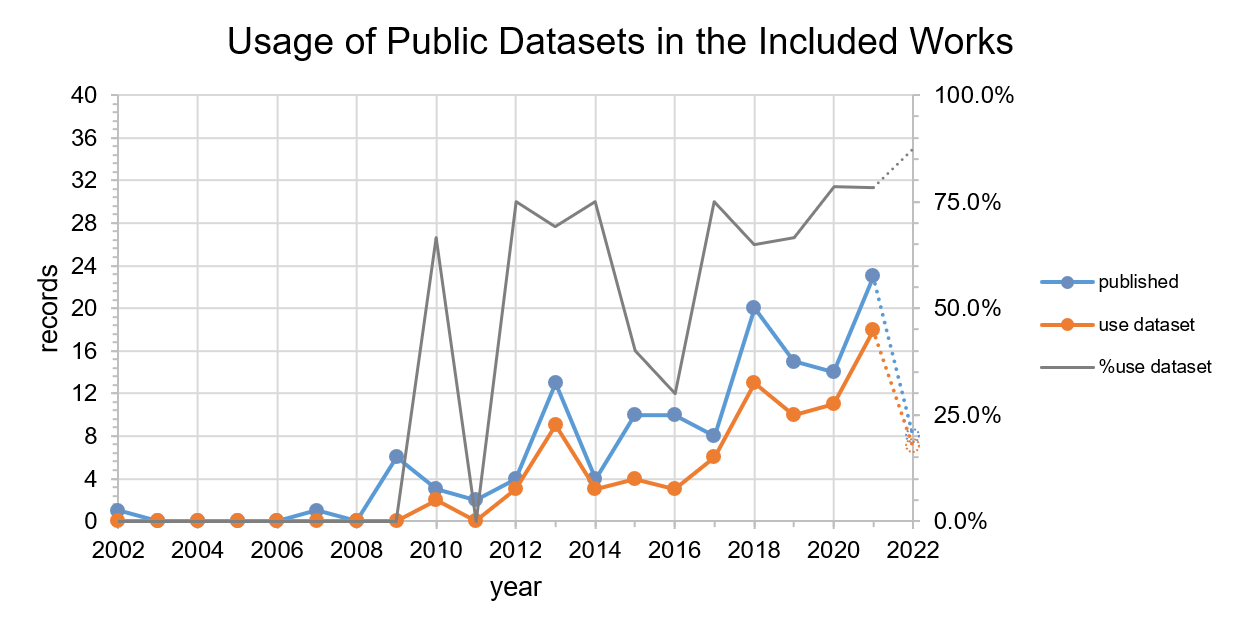
\includegraphics[width=\columnwidth]{figures/datasets.png}
  \caption{Evolution of the usage of public datasets per year considering the 142 included records in this review.}
  \label{fig:discussion:datasets}
\end{figure}

Although DE11 indicates which datasets are used in the experiments, this item does not characterize the datasets. Thus, Table~\ref{tab:discussion:datasets} presents a comparison table with the following items: long-term characteristics of the dataset in terms of the environment conditions (lighting, day and night sequences, weather and seasonal changing conditions, dynamic elements, and sparsity), type of environment (indoor, outdoor, or both), the domain of the agent used for acquiring data (ground, air, or water, and the commercial unit used if indicated), sensorization, if the dataset provides intrinsic and extrinsic calibration of the sensor setup used, type of ground-truth data, format, and long-term characteristics in terms of distance, time, and the number of runs. Next, the discussion focuses on comparing the datasets based on the column items presented in Table~\ref{tab:discussion:datasets} and correlating their usage in terms of DE1.

\onecolumn

\renewcommand{\arraystretch}{1.125}
\setlength{\tabcolsep}{1.5pt}

\begin{tiny}

\begin{longtable}{@{\extracolsep{1pt}}
p{0.065\textwidth}                          % Dataset name
c|                                          % Year
cccccc|                                     % Long-term
p{0.095\textwidth}                          % Environment
p{0.095\textwidth}|                         % Domain
c|                                          % Sensory setup: odo
ccccccc|                                    %                camera
cc|                                         %                laser
cccc|                                       %                radar, sonar, imu, gps
cc|                                         % Sensor calibrations
p{0.095\textwidth}p{0.095\textwidth}|       % Ground-truth + Format
ccccc@{}}                                   % Distance, time, \#sequences
  \caption{Datasets used in the 144 included records for long-term localization and / or mapping experiments. Legend: odo -- odometry (wheeled, laser, visual, inertial, or a combination of odometry sources, dist. -- total distance length of the dataset, path -- total path distance if repeated several times, time -- total operation time, int. -- time interval between the start and end acquisition dates / time instants (d/w/m/y equivalent to day/week/month/year, 0 if only 1 run), and seq. -- number of sequences of the dataset.}
  %\vspace{0.5em}
  \label{tab:discussion:datasets}\\

%% FIRST TABLE HEADER
\hline
&&
\multicolumn{6}{c|}{\textbf{Long-term}} &
&&
\multicolumn{14}{c|}{\textbf{Sensor}} &
\multicolumn{2}{c|}{\textbf{Calib.}} &
&&
&&&&\\
&&&&&&&&&&
\multicolumn{1}{c}{} &
\multicolumn{7}{c}{\textbf{camera}} &
\multicolumn{2}{c}{\textbf{laser}}  &
&&&&
&&
&&
&&&&\\
\cline{12-18}
\cline{19-20}
\textbf{Dataset} & \textbf{Year} &
\rotatebox{90}{\textbf{lighting}} & \rotatebox{90}{\textbf{day/night}} & \rotatebox{90}{\textbf{weather}} & \rotatebox{90}{\textbf{seasonal}} & \rotatebox{90}{\textbf{dynamics}} & \rotatebox{90}{\textbf{sparsity}} & 
\textbf{Environ.} & \textbf{Domain} & 
\multicolumn{1}{c}{\rotatebox{90}{\textbf{odo}}} &
\rotatebox{90}{\textbf{gray}} & \rotatebox{90}{\textbf{color}} & \rotatebox{90}{\textbf{monocular}} & \rotatebox{90}{\textbf{stereo}} & \rotatebox{90}{\textbf{omni}} & \rotatebox{90}{\textbf{RGBD}} & \multicolumn{1}{c}{\rotatebox{90}{\textbf{thermal}}} &
\rotatebox{90}{\textbf{2D}} & \multicolumn{1}{c}{\rotatebox{90}{\textbf{3D}}} &
\rotatebox{90}{\textbf{radar}} & \rotatebox{90}{\textbf{sonar}} & \rotatebox{90}{\textbf{IMU}} & \rotatebox{90}{\textbf{GPS}} &
\rotatebox{90}{\textbf{intrinsic}} & \rotatebox{90}{\textbf{extrinsic}} & 
\textbf{GT data} & \textbf{Format} & 
\rotatebox{90}{\textbf{dist.} (km)} & \rotatebox{90}{\textbf{path} (km)} & \rotatebox{90}{\textbf{time} (h)} & \rotatebox{90}{\textbf{int.} (d/w/m/y)} & \rotatebox{90}{\textbf{\#seq.}}\\
\hline
\endfirsthead

%% TABLE HEADER IN THE FOLLOWING PAGES
\multicolumn{27}{l}{\itshape{\tablename\ \thetable{}: continued from previous page}}
\vspace{0.5em}\\
\hline
&&
\multicolumn{6}{c|}{\textbf{Long-term}} &
&&
\multicolumn{14}{c|}{\textbf{Sensor}} &
\multicolumn{2}{c|}{\textbf{Calib.}} &
&&
&&&&\\
&&&&&&&&&&
\multicolumn{1}{c}{} &
\multicolumn{7}{c}{\textbf{camera}} &
\multicolumn{2}{c}{\textbf{laser}}  &
&&&&
&&
&&
&&&&\\
\cline{12-18}
\cline{19-20}
\textbf{Dataset} & \textbf{Year} &
\rotatebox{90}{\textbf{lighting}} & \rotatebox{90}{\textbf{day/night}} & \rotatebox{90}{\textbf{weather}} & \rotatebox{90}{\textbf{seasonal}} & \rotatebox{90}{\textbf{dynamics}} & \rotatebox{90}{\textbf{sparsity}} & 
\textbf{Environ.} & \textbf{Domain} & 
\multicolumn{1}{c}{\rotatebox{90}{\textbf{odo}}} &
\rotatebox{90}{\textbf{gray}} & \rotatebox{90}{\textbf{color}} & \rotatebox{90}{\textbf{monocular}} & \rotatebox{90}{\textbf{stereo}} & \rotatebox{90}{\textbf{omni}} & \rotatebox{90}{\textbf{RGBD}} & \multicolumn{1}{c}{\rotatebox{90}{\textbf{thermal}}} &
\rotatebox{90}{\textbf{2D}} & \multicolumn{1}{c}{\rotatebox{90}{\textbf{3D}}} &
\rotatebox{90}{\textbf{radar}} & \rotatebox{90}{\textbf{sonar}} & \rotatebox{90}{\textbf{IMU}} & \rotatebox{90}{\textbf{GPS}} &
\rotatebox{90}{\textbf{intrinsic}} & \rotatebox{90}{\textbf{extrinsic}} & 
\textbf{GT data} & \textbf{Format} & 
\rotatebox{90}{\textbf{dist.} (km)} & \rotatebox{90}{\textbf{path} (km)} & \rotatebox{90}{\textbf{time} (h)} & \rotatebox{90}{\textbf{int.} (d/w/m/y)} & \rotatebox{90}{\textbf{\#seq.}}\\
\hline
\endhead

%% TABLE FOOTER
\hline
\endfoot
\hline
\endlastfoot



\citetitle{dataset:fhw} & 2001 &  &  &  &  &  & x & indoor (museum) & ground (TOURBOT) & x &  &  &  &  &  &  &  & x &  &  &  &  &  &  &  & -- & CARMEN & -- & -- & 1.98 & -- & 1\\
\hline
\citetitle{dataset:fr079} & 2003 &  &  &  &  &  & x & indoor (office) & ground (robot) & x &  &  &  &  &  &  &  & x &  &  &  &  &  &  &  & -- & CARMEN & -- & -- & 0.29 & -- & 1\\
\hline
\citetitle{dataset:fr101} & 2003 &  &  &  &  &  & x & indoor (office) & ground (robot) & x &  &  &  &  &  &  &  & x &  &  &  &  &  &  &  & -- & CARMEN & -- & -- & 0.29 & -- & 1\\
\hline
\citetitle{dataset:intel03} & 2003 &  &  &  &  &  & x & indoor (office) & ground (robot) & x &  &  &  &  &  &  &  & x &  &  &  &  &  &  &  & -- & CARMEN & 0.506 & -- & 0.75 & -- & 1\\
\hline
\citetitle{dataset:mit-kilian} & 2004 &  &  &  &  &  & x & indoor (office) & ground (robot) & x &  &  &  &  &  &  &  & x &  &  & x &  &  &  &  & -- & CARMEN & 2.2 & -- & 2.5 & -- & 1\\
\hline
\citetitle{dataset:city-center-fabmap} & 2008 & x &  &  &  & x &  & outdoor (urban) & ground (robot) &  &  & x & x &  &  &  &  &  &  &  &  &  & x & x &  & GPS, manual & plain text (non-image), jpg (image) & 2 & -- & -- & -- & 1\\
\hline
\citetitle{dataset:lip6indoor} & 2008 &  &  &  &  &  &  & indoor (office) & ground (handheld) &  &  & x & x &  &  &  &  &  &  &  &  &  &  & x &  & manual & ppm (images) & -- & -- & 0.11 & -- & 1\\
\hline
\citetitle{dataset:lip6outdoor} & 2008 & x &  &  &  & x &  & outdoor (campus) & ground (handheld) &  &  & x & x &  &  &  &  &  &  &  &  &  &  & x &  & manual & ppm (images) & -- & -- & 0.3 & -- & 1\\
\hline
\citetitle{dataset:new-college-fabmap} & 2008 & x &  &  &  & x &  & outdoor (campus) & ground (robot) &  &  & x & x &  &  &  &  &  &  &  &  &  & x & x &  & GPS, manual & plain text (non-image), jpg (image) & 1.9 & -- & -- & -- & 1\\
\hline
\citetitle{dataset:stlucia07} & 2008 & x &  &  &  & x &  & outdoor (urban) & ground (car) &  & x &  & x &  &  &  &  &  &  &  &  &  &  &  &  & -- & -- & 66 & -- & 1.67 & -- & 1\\
\hline
\citetitle{dataset:bicocca-indoor} & 2009 & x &  &  &  & x & x & indoor (office) & ground (Robocom) & x & x & x & x & x & x &  &  & x &  &  & x & x &  & x & x & map model, laser-based & plain text (non-image), png (image) & -- & -- & 2.5 & 3d & 5\\
\hline
\citetitle{dataset:cold} & 2009 & x & x & x &  & x &  & indoor (office) & ground (Pioneer 3, ATRV Mini, PeopleBot) & x &  & x & x &  & x &  &  & x &  &  &  &  &  &  &  & laser-based, manual & plain text (non-image), jpg (image) & 0.92 & -- & 0.99 & -- & 76\\
\hline
\citetitle{dataset:malaga-2009} & 2009 & x &  &  &  & x &  & outdoor (parking, campus) & ground (car) &  &  & x & x &  &  &  &  & x &  &  &  & x & x & x & x & RTK-GPS & Rawlog MRPT & 6.358 & -- & -- & -- & 6\\
\hline
\citetitle{dataset:newcollege} & 2009 & x &  &  &  & x &  & outdoor (campus) & ground (Segway) & x & x & x &  & x & x &  &  & x &  &  &  & x & x & x & x & GPS & plain text (non-image), png (stereo), jpg (omni) & 2.2 & -- & 0.73 & -- & 1\\
\hline
\citetitle{dataset:albert-b} & 2010 & x &  &  &  &  & x & indoor (office) & ground (iRobot B21r) & x &  & x & x &  &  &  &  & x &  &  &  &  &  &  &  & -- & CARMEN (non-image), jpg (image) & -- & -- & 0.18 & -- & 1\\
\hline
\citetitle{dataset:cmu-vl} & 2011 & x &  &  & x & x &  & outdoor (urban) & ground (car) &  &  & x & x &  &  &  &  &  &  &  &  &  & x & x & x & GPS & -- & -- & 8.5 & -- & 1y & 16\\
\hline
\citetitle{dataset:ford} & 2011 & x &  &  &  & x &  & outdoor (campus, urban) & ground (car) &  &  & x &  &  & x &  &  & x & x &  &  & x & x & x & x & RTK-GPS & LCM log & -- & -- & -- & 2m & --\\
\hline
\citetitle{dataset:utias} & 2011 & x &  &  &  &  &  & indoor (empty space) & ground (iRobot Create) & x &  & x & x &  &  &  &  &  &  &  &  &  &  & x &  & external tracking system & jpg (image), dat (non-image) & -- & -- & 4.78 & -- & 9\\
\hline
\citetitle{dataset:alderley} & 2012 & x &  & x &  & x &  & outdoor (urban) & ground (car) &  &  & x & x &  &  &  &  &  &  &  &  &  &  &  &  & manual & -- & 16 & 8 & -- & -- & 2\\
\hline
\citetitle{dataset:tum-rgbd} & 2012 & x &  &  &  & x &  & indoor (office, industrial hall) & ground (handheld, Pioneer 3) &  &  & x &  &  &  & x &  &  &  &  &  & x &  & x & x & external tracking system & plain text (non-image), png (image + depth), ROS bag & 0.285 & -- & 0.35 & -- & 15\\
\hline
\citetitle{dataset:cobot} & 2013 & x &  &  & x & x & x & indoor (office) & ground (robot) & x &  & x &  &  &  & x &  & x &  &  &  &  &  &  & x & -- & ROS bag & 131 & -- & 260 & 2y3m & 1082\\
\hline
\citetitle{dataset:kitti} & 2013 & x &  &  &  & x &  & outdoor (urban) & ground (car) &  & x & x & x & x &  &  &  &  & x &  &  & x & x & x & x & RTK-GPS & png (image), binary (laser), plain text (imu, gps) & -- & -- & 1.18 & 8d & 61\\
\hline
\citetitle{dataset:mit-stata} & 2013 & x &  &  & x & x & x & indoor (office) & ground (PR2) & x &  & x &  & x &  & x &  & x &  &  &  & x &  &  & x & map model & ROS bag & 42 & -- & 38 & 1y9m & 84\\
\hline
\citetitle{dataset:nordlandsbanen} & 2013 & x &  & x & x &  &  & outdoor (railway) & ground (train) &  &  & x & x &  &  &  &  &  &  &  &  &  & x &  &  & GPS & mp4 (video stream), plain text (gps) & 2916 & 729 & 39.74 & -- & 4\\
\hline
\citetitle{dataset:gardens-qut} & 2014 & x & x &  &  & x &  & indoor, outdoor (campus) & ground (handheld) &  &  & x & x &  &  &  &  &  &  &  &  &  &  &  &  & ground-plane position & png (images), plain text (ground plane) & -- & -- & -- & -- & 3\\
\hline
\citetitle{dataset:lcas-strands} & 2014 & x & x &  & x & x &  & indoor (office) & ground (SCITOS-G5) &  &  & x &  &  &  & x &  & x &  &  &  &  &  &  & x & -- & ROS bag & -- & -- & -- & 1y1m & 368\\
\hline
\citetitle{dataset:kaist} & 2015 & x & x &  &  & x &  & outdoor (urban) & ground (car) &  &  & x &  & x &  &  & x &  &  &  &  & x & x & x & x & RTK-GPS & png (images), plain text (imu, gps) & 84 & -- & -- & 18d & 36\\
\hline
\citetitle{dataset:euroc} & 2016 & x &  &  &  &  &  & indoor (industrial hall, office) & air (AscTec Firefly) &  & x &  & x & x &  &  &  &  &  &  &  & x &  & x & x & external tracking system & ROS bag & 0.8936 & -- & 0.37 & -- & 11\\
\hline
\citetitle{dataset:nclt} & 2016 & x &  & x & x & x &  & indoor, outdoor (campus) & ground (Segway) &  &  & x &  &  & x &  &  & x & x &  &  & x & x & x & x & RTK-GPS, SLAM-based & binary (laser), tiff (image), plain text (non-laser or image) & 147.4 & -- & 34.9 & 1y4m & 27\\
\hline
\citetitle{dataset:kudamm} & 2017 & x &  &  &  & x &  & outdoor (urban) & ground (car) &  &  & x & x &  &  &  &  &  &  &  &  &  &  &  &  & manual & jpg (image) & -- & -- & -- & -- & 2\\
\hline
\citetitle{dataset:oxford-robotcar} & 2017 & x & x & x & x & x &  & outdoor (urban) & ground (car) & x &  & x & x & x &  &  &  & x & x &  &  & x & x & x & x & RTK-GPS & png (image), binary (laser), plain text (imu, gps, odo) & 1010.46 & 10 & -- & 1y8m & 133\\
\hline
\citetitle{dataset:yq21} & 2017 & x &  &  &  & x &  & outdoor (campus) & ground (car) &  &  & x & x & x &  &  &  &  & x &  &  & x & x & x & x & RTK-GPS & binary (laser), jpg (images), plain text (gps) & 23 & -- & 6.5 & 1w & 21\\
\hline
\citetitle{dataset:cmu-seasons} & 2018 & x &  &  & x & x &  & outdoor (urban) & ground (car) &  &  & x & x &  &  &  &  &  &  &  &  &  &  & x & x & manual & jpg (image) & -- & 8.5 & -- & 330d & 17\\
\hline
\citetitle{dataset:fas} & 2018 & x &  &  & x & x &  & outdoor (urban) & ground (car) &  &  & x &  & x &  &  &  &  &  &  &  &  & x &  &  & GPS, manual & jpg (image) & 110 & -- & -- & 3y & 3\\
\hline
\citetitle{dataset:robotcar-seasons} & 2018 & x &  & x &  & x &  & outdoor (urban) & ground (car) &  &  & x & x & x &  &  &  &  &  &  &  &  &  & x & x & manual & jpg (image) & -- & 10 & -- & 178d & 10\\
\hline
\citetitle{dataset:bonn} & 2019 &  &  &  &  & x &  & indoor (office) & ground &  &  & x &  &  &  & x &  &  &  &  &  &  &  & x & x & external tracking system & png (images, depth), plain text (imu, gps) & -- & -- & -- & -- & 26\\
\hline
\citetitle{dataset:cbd} & 2019 & x &  &  &  & x &  & outdoor (urban) & ground &  &  & x & x & x &  &  &  &  &  &  &  &  &  &  &  & manual & png (images) & -- & -- & -- & -- & 1\\
\hline
\citetitle{dataset:mulran} & 2020 &  &  &  &  & x &  & outdoor (urban) & ground (car) &  &  &  &  &  &  &  &  &  & x & x &  & x & x &  & x & SLAM-based & binary (laser), CSV (global pose, radar ray), png (radar polar image) & 41.2 & -- & -- & 2m15d & 12\\
\hline
\citetitle{dataset:robotcar-radar} & 2020 & x &  & x &  & x &  & outdoor (urban) & ground (car) & x &  & x & x & x &  &  &  &  & x & x &  & x & x & x & x & RTK-GPS, SLAM-based & png (image, raw laser, radar), binary (laser), plain text (imu, gps, odo) & 280 & 10 & -- & 1m & 32\\
\hline
\citetitle{dataset:usyd} & 2020 & x &  & x & x & x &  & outdoor (campus) & ground (car) & x &  & x & x &  &  &  &  &  & x &  &  & x & x & x & x & GPS & ROS bag & -- & -- & -- & 1y & 52\\
\hline
\citetitle{dataset:iplt} & 2021 & x & x & x & x & x &  & outdoor (parking) & ground (car) & x & x &  & x &  &  &  &  & x &  &  &  &  & x & x & x & GPS & ROS bag & -- & 0.2 & -- & 2y & 127\\
\hline
\citetitle{dataset:radiate} & 2021 & x & x & x &  & x &  & outdoor (parking, urban) & ground (car) &  &  & x & x & x &  &  &  &  & x & x &  & x & x & x & x & RTK-GPS & ROS bag & -- & -- & 4.98 & -- & --\\
\hline
\citetitle{dataset:ntu} & 2022 & x &  &  &  &  &  & indoor, outdoor (campus) & air (DJI M600) &  & x &  & x & x &  &  &  &  & x &  &  & x &  & x & x & external tracking system & ROS bag & 1.845 & -- & 0.9 & -- & 9\\



%  \end{tabular}}
%\end{table*}
\end{longtable}

\end{tiny}

\twocolumn

\renewcommand{\arraystretch}{1.25}
\setlength{\tabcolsep}{3pt}



\paragraph{Environment}

The outdoor environment is the most seen one in the 43 datasets, with 27 being acquired outdoors compared to 19 indoors, and 3 datasets (\citetitle{dataset:gardens-qut}, \citetitle{dataset:nclt}, and \citetitle{dataset:ntu}) having indoor and outdoor sequences.
The environment changing conditions more present in indoor datasets are lighting changes and dynamic elements, e.g., in office environments where the exterior and artificial light influence the visual perception and moving people increase environment dynamics (not only the people, but moving objects taken by persons).
Although night periods, weather and seasonal changes also influence indoor conditions, this influence is mostly in the lighting conditions and only appear in 4 indoor-only datasets (\citetitle{dataset:cold}, \citetitle{dataset:cobot}, \citetitle{dataset:mit-stata}, and \citetitle{dataset:lcas-strands}), accordingly to the respective dataset descriptions.
Similarly, the outdoor datasets are more affected by changing lighting and moving objects. However, these datasets consider more frequently and are more influenced by other changes. This influence is not only in lighting conditions but also in visual perception (color of the leaves in different seasons) and moving elements in the scene (water of the rain or moving tree branches due to strong wind).
In terms of recency, in the past 5 years, only 2 of the 14 datasets released during that period are in indoor locations. This recent tendency and the fact of 27/43 datasets having outdoor sequences indicate more interest in this type of environment by the included works in this review.

As for the diversity of the acquisition conditions, the most diverse datasets are \citetitle{dataset:cold}, \citetitle{dataset:lcas-strands}, \citetitle{dataset:nclt}, \citetitle{dataset:usyd}, \citetitle{dataset:radiate}, \citetitle{dataset:iplt}, and \citetitle{dataset:oxford-robotcar}. The latter two have all changing conditions in the environment, i.e., lighting, day/night sequences, dynamic elements, and weather and seasonal changes. Even though the remaining diverse datasets do not consider one of these conditions, the datasets are still interesting in the long-term localization and mapping context with a high diversity of environment conditions.

The datasets categorized as sparsity are intended for testing map maintenance algorithms to constrain the graph size in the graph SLAM formulation to the operation area and not to the trajectory length due to usually being available the full graph map of the dataset. Although these datasets are useful for evaluating map maintenance, they normally lack several other changing conditions that influence long-term localization and mapping while also all of those datasets being indoors. Only \citetitle{dataset:cobot} and \citetitle{dataset:mit-stata} datasets seem to be more diverse in terms of environment conditions by capturing sequences with different lighting conditions and dynamic elements in the scene.


\paragraph{Sensorization}

In terms of the type of sensors used for acquiring data, the ones utilized in the datasets are odometry (wheeled, visual, inertial, laser, or a combination of different odometric sources), cameras (monocular, stereo, omnidirectional, RGBD, or thermal), lasers (2D/3D), radar, sonar, IMU, and GPS, similar to the sensors found in the data extraction phase of this review. The more common type of sensor is camera used in 37/43 (86\%) datasets. This predominance is conformal with the high usage in 104/142 (73.2\%) included works and occurrence of related keywords in the analysis presented in Figure~\ref{fig:overview:kw} (both vision and camera keywords appear in the graph with 18 and 7 occurrences, respectively), indicating an interest of using camera sensors in data acquisition and long-term localization and mapping.
Also, the omnidirectional vision used in 5 datasets can be accomplished by using an hyperbolic mirror (\citetitle{dataset:bicocca-indoor}, \citetitle{dataset:cold}), joining the image of several cameras and using their extrinsic calibrated parameters, or using an omnidirectional camera (\citetitle{dataset:ford}, \citetitle{dataset:nclt}, \citetitle{dataset:newcollege}) such as the Point Grey LadyBug 2 5-view.
Although the thermal camera is only present in \citetitle{dataset:kaist}, this sensor can be interesting for building inspection \parencite{yue-et-al:2020:9197072}.

Moreover, datasets used in the included works recently released also use 3D laser (or LiDAR) and radar sensors. Although the older dataset with 3D laser is from 2011 (\citetitle{dataset:ford}), 5/10 (50\%) datasets using this sensor were released over the past 5 years from a total of 14 datasets released in this same period. This trend is noted also when analyzing the DE7 item of the included works, where 24/27 (89\%) methods using a 3D laser were proposed since 2018, indicating a recent importance of this sensor for long-term localization and mapping.
As for radar data, all 3 datasets using the sensor (\citetitle{dataset:mulran}, \citetitle{dataset:robotcar-radar}, and \citetitle{dataset:radiate}) were released since 2020. A corresponding recency is noted in included works with 3/4 (75\%) methods (\cite{martini-et-al:2020:s20216002}, \cite{yin-et-al:2021:661199}, and \cite{hong-et-al:2022:02783649221080483}) using the sensor are also from 2020 onwards. This recent usage indicates a recent interest of using radar data within the scope of this review's topic, probably due to being less affected by changing lighting or weather conditions compared to visual sensors~\parencite{hong-et-al:2022:02783649221080483}.

As for the other sensors used in the dataset, odometry data, IMU, 2D laser, and GPS are also extensively used in the datasets.
The first two provide relative motion information of the vehicle and are used in 16 and 17 datasets and 33 and 19 included works, respectively.
Although the 2D laser is used in 17 datasets, 15 of those are from 2016 and previous years. However, the sensor is still used in the included works over the years, especially in indoor environments, with 21/25 works for indoors using 2D lasers.
As for GPS data, this sensor is usually used as ground-truth data, as will be discussed later.

Sensor calibration is important for achieving long-term localization and mapping, not only for avoiding the propagation of inconsistency pose errors between sensors through time, but also to process the perceived data from the environment in the same coordinate referential frame. The intrinsic calibration is usually relative to camera sensors, where 25/37 (68\%) datasets with this sensor provide the intrinsic parameters to the user. Some of the datasets with cameras do not provide those parameters due to being intended only for image-based place recognition (e.g., \citetitle{dataset:city-center-fabmap}, \citetitle{dataset:cbd}, or \citetitle{dataset:fas}).
In terms of extrinsic calibration, 24/43 (56\%) datasets provide these parameters, being useful for evaluating methods where the parameters are required to be processed in the same reference frame.

The datasets more diverse in terms of their sensor setup are \citetitle{dataset:bicocca-indoor}, \citetitle{dataset:oxford-robotcar}, and \citetitle{dataset:robotcar-radar}, with 7, 6, and 6 different types of sensors, respectively.


\paragraph{File format}

Most of the datasets used by the included works define a specific format for organizing the respective data. These formats use standard file types such as plain text, CSV, or binary files having the advantage of not being tied to any particular software. Even so, there are common characteristics between those specific formats.
Images are usually saved in JPG or PNG files, whereas PNG files are also used in the datasets for saving depth information of RGBD sensors.
The laser data is usually saved in binary files due to its easiness for parsing by different programming languages and size considerations~\parencite{dataset:kitti,dataset:oxford-robotcar}.
Another common aspect of specific formats found in the datasets of Table~\ref{tab:discussion:datasets} is the use of plain text or CSV files to save IMU, GPS, and/or odometry data.
As for radar data, the respective polar representations are saved in PNG files.

However, the datasets also make available standard log formats compatible with different types of sensor data.
The most used one is ROSbag from the Robot Operating System (ROS) framework in 9 datasets. This log format is compatible with common messages defined in ROS for different sensors\footnote{\url{http://wiki.ros.org/common_msgs}}.
The other standard format used in more than one dataset is CARMEN log files defined in the CARMEN robot navigation toolkit\footnote{\url{https://carmen.sourceforge.net/}}. Although this log format supports different sensor data such as odometry or lasers, the CARMEN navigation toolkit is not updated since 2008 (version 0.7.4-beta), considered to be deprecated.


\paragraph{Usage relation with the included records}

As for relating the datasets usage with this review's included works, the datasets can be related with the DE1 categorization of the records. From the appearance category in DE1, 50/75 (67\%) works use 32 different public datasets from Tabl~\ref{tab:discussion:datasets} to evaluate the proposed methodologies. The datasets most used are \citetitle{dataset:kitti}, \citetitle{dataset:nordlandsbanen}, \citetitle{dataset:nclt}, \citetitle{dataset:stlucia07}, and \citetitle{dataset:oxford-robotcar} (13, 11, 9, 8, and 8 usages). \citetitle{dataset:kitti} is also the most used overall, given the 26 works utilizing it for evaluation. However, this dataset and \citetitle{dataset:stlucia07} do not have seasonal nor weather changing conditions that greatly influence the appearance invariance of the methods, as discussed in Section~\ref{sec:discussion:appearance}, even though those datasets have high usage by the appearance-related works. Indeed, more recent datasets such as \citetitle{dataset:nclt} or \citetitle{dataset:oxford-robotcar} already widely used for evaluation, or also \citetitle{dataset:usyd} and \citetitle{dataset:radiate} would be suitable for evaluating the appearance invariance of the localization and mapping algorithms due to the datasets' diversity in terms of varying conditions.

Although the works categorized as dynamics and sparsity also use public datasets for evaluation, the usage is slightly lower than for appearance-related methods (44\% and 51\%, respectively, compared to 67\%).
\citetitle{dataset:kitti}, \citetitle{dataset:tum-rgbd}, and \citetitle{dataset:lcas-strands} are the only datasets used in more than one work categorized as dynamic (7, 6, and 2 usages, respectively), considering a total of 10 different datasets used by these works. However, \citetitle{dataset:kitti} and \citetitle{dataset:tum-rgbd} could be not the most suitable datasets for evaluating the performance over different levels of dynamics in the environment due to the smaller total operation time of 1.18h and 0.35h, respectively, compared to other datasets classified as having dynamic elements in Table~\ref{tab:discussion:datasets}. For example, \citetitle{dataset:lcas-strands} has a time frame of 1 year and a month in an indoor office environment capturing different motion frequencies or habits of the persons working at the scene with an average of 1 daily acquisition run. \citetitle{dataset:oxford-robotcar} and \citetitle{dataset:usyd} are also interesting due to the long time frames of the data acquisition (1 year and 8 months, and 1 year, with 133 and 52 runs, respectively). Also, \citetitle{dataset:iplt} is captured in a parking lot environment capturing semi-static and dynamic moving cars in the scene.
As for sparsity-related works, 22 different datasets are used in the experiments, whereas \citetitle{dataset:kitti}, \citetitle{dataset:intel03}, \citetitle{dataset:mit-kilian}, \citetitle{dataset:mit-stata}, and \citetitle{dataset:euroc} being the most utilized ones (6, 5, 3, 3, and 3 usages, respectively). \citetitle{dataset:kitti} and \citetitle{dataset:euroc} are used for evaluating feature management techniques, though these datasets have small operation time frames and, possibly, trajectory lengths. Although \citetitle{dataset:mit-stata} would seem like a good dataset for evaluating the sparsity due to the long trajectory length and time frame (42km and 38h, respectively), the dataset's description indicates that hardware and calibration problems in the data acquisition setup may have created inconsistencies in the data. As for \citetitle{dataset:intel03}, \citetitle{dataset:mit-kilian}, and other datasets classified as sparsity in Table~\ref{tab:discussion:datasets}, these are widely used for graph sparsification due to repeated passages in same locations with a total of 15 usages, even though those datasets have usually only 1 data sequence. Other recent datasets could also be interesting for evaluation sparsification techniques of the map such as \citetitle{dataset:oxford-robotcar} and \citetitle{dataset:mulran}, given the repeated passages over the 10km path and the long trajectory length of 41.2km, respectively.

Furthermore, 5/7 multi-session works used datasets, whereas the \citetitle{dataset:mit-stata} and \citetitle{dataset:intel03} being the most used ones with 2 usages each. While each data sequence of \citetitle{dataset:mit-stata} may represent a single session~\parencite{lázaro-et-al:2018:8594310}, the unique data sequence of \citetitle{dataset:intel03} can be split into different sessions~\cite{latif-et-al:2012:6385879}. This approach is valid for applying to other datasets in Table~\ref{tab:discussion:datasets}.
As for the computational categorization on DE1, this category does not relate to the datasets used in the experiments because the computational efficiency is more dependent on the proposed localization and/or mapping algorithm than on the data.

In terms of multi-robot works~\parencite{gadd-newman:2016:7759843,zhang-et-al:2018:1729881418780178,karaoguz-bozma:2020:2,yue-et-al:2020:9197072} identified by the DE4, even though the dataset \citetitle{dataset:utias} collects data from 5 robots and being the only multi-robot dataset in Table~\ref{tab:discussion:datasets}, it is only used in \cite{nobre-et-al:2018:8461111} to test the reconfiguration of landmarks in the scene in different runs for single-robot localization and mapping. The only datasets used in multi-robot works are \citetitle{dataset:kitti} in \cite{zhang-et-al:2018:1729881418780178} and \citetitle{dataset:cold} in \cite{karaoguz-bozma:2020:2}. These works assume that different data sequences are acquired by different agents or segment the sequence in data subsets, similar to the evaluation with datasets of multi-session works.
However, the fact that only 4 multi-robot works are included in this review and only 1 public dataset used in the included records is acquired with multiple vehicles could indicate that the use of multi-robot systems is not yet widely studied in the long-term localization and mapping topic.



\subsubsection{Distance and time considerations}

Next, analyzing the total trajectory length of the private experiments on the included records (DE10 on Table~\ref{tab:a2:data-extraction}) and public datasets (see Table~\ref{tab:discussion:datasets}), 5 works and 6 datasets have a length greater than 100km.
Higher values on the trajectory length indicate possibly more interesting data for evaluating sparsity management techniques discussed in Section~\ref{sec:discussion:sparsity}, given that the desired behavior of a mapping algorithm is its scalability being only dependent on the environment size and not on the trajectory length. Although the total trajectory length does not necessarily relates directly with the environment area, the latter is rarely seen in the experiments description, and even for the trajectory length, only 36/77 works that perform private experiments and 22/43 datasets indicate the length.

The other distance measure considered in this review to characterize the experimental data is the one relative to repeating the same path, with 7/8 datasets and 3/8 included works that specify this metric having a repetitive path distance greater than 8km and more than 1 run. These low numbers do not necessarily indicate incomplete information in the experimental description due to a data acquisition can be performed on non-repetitive routes. Even so, repeating the same exact path under different environment conditions (i.e., appearance variance) could be a case study for evaluating the appearance invariance of localization and mapping algorithms discussed in Section~\ref{sec:discussion:appearance}.

In terms of time-related long-term characteristics of experimental data, longer total operation times indicate a robust evaluation of the proposed localization and mapping algorithms over long continuous periods, and greater time interval suggests data acquired under severe changing conditions (not only in the environment appearance but also semi-static modifications in the scene). However, only 2/10 works performing private experiments and indicating the total operation time test their methods over a total of 8h (equivalent to a work day), while also only 4/23 datasets that define the total log time in their description have more than 8h of data. On the contrary, 41/77 works and 18/43 datasets characterize the interval between the first and the last data sequence, which of those 29 works performing private experiments and 17 datasets have at least a 1 week interval. These results indicate that even though the included works in this review use experimental data with greater time intervals, often several days or weeks, not so much importance is given towards the total operation time.



\subsubsection{Ground-truth data}

As for the types of ground-truth data found in the included works (see DE9 in Table~\ref{tab:a2:data-extraction}) and the public datasets used for evaluation (see Table~\ref{tab:discussion:datasets}), the manual annotation is one of the most used types of ground-truth including image to image association (e.g., useful for evaluating image-based place recognition), manual alignment of maps~\parencite{biswas-veloso:2013:0278364913503892}, or manually segmenting images~\parencite{dataset:kitti}.
Although GPS-based data is also widely used in the experiments, whereas the RTK-GPS variant improves the pose precision compared to the basic positioning system, GPS is meant for use in outdoor environments. The alternative for indoor environments used in the experiments is external tracking systems using, e.g., reflective markers put on the robot to track them through systems such as OptiTrack\footnote{\url{https://optitrack.com/}} or Vicon\footnote{\url{https://www.vicon.com/}} to provide precise measurements of the robot's pose.
Simulation data used in 10 included works can also provide precise ground-truth data for the robot's pose or other types of information, even though not in a real environment.

Moreover, SLAM or laser-based ground-truth data are also found in the experimental evaluation of the included works and public datasets. The experimental methodology uses localization and mapping algorithms other than the one being evaluated to provide ground-truth data usually using a different sensor setup, or using the same algorithm but including all data sessions or global optimization over the entire pose graph.
Specifically, laser-based localization is widely used in the included works as ground-truth data to evaluate vision-based methods~\parencite{nuske-et-al:2009:20306}.
Similarly to SLAM-based ground-truth data, the experimental results of localization and mapping methods without pruning are also used as a reference for evaluating sparsification algorithms~\parencite{carlevaris-bianco-et-al:2014:2347571}.

As for model-based ground-truth data, the work of \cite{boniardi-et-al:2019:003} and the datasets \citetitle{dataset:bicocca-indoor} and \citetitle{dataset:mit-stata} propose the use of floor plans as a model of the environment to align the current estimation with the model and obtain a ground-truth for the trajectory of the robot on the map.
\cite{ozog-et-al:2016:21582}  is the other method using map models in the experimental evaluation but in the context of ship hull inspection, where the current map estimation is aligned with the ship hull CAD model for obtaining the trajectory ground-truth data.
However, the use of map-based ground-truth data to evaluate the mapping process is not seen in the included works, other than performing a visual quality evaluation over the mapping results and the sensor data.





\subsection{Evaluation metrics}
\label{sec:discussion:metrics}

The final topic of discussion over the included works in this review is the analysis on evaluation metrics used for assessing the performance of the proposed methodologies (see DE12 in Table~\ref{tab:discussion:datasets}).
This analysis is organized by metrics intended for place recognition, evaluation of the robot pose, assessment of map sparsity, and computational performance.



\subsubsection{Place recognition}

The evaluation of place recognition performance within the context of this review is intrinsically related to the invariance to changing conditions of long-term localization and mapping, and so, works categorized as appearance in DE1. The most used metrics for place recognition in the included works are precision and recall, where 50/142 works use these metrics in the experimental evaluation, and from those works 39 are categorized as appearance. These metrics characterize the performance of recognizing successfully different places related to the number of true and false positives and true and false negatives, and also include the precision-recall curve where a greater area under the curve indicates a better classifier for place recognition.

Other metrics less used in the included works but also important are the confusion matrix, the localization success rate, and the f-score and f-beta measures. The confusion matrix associates the predicted place to the true value in the case of each data entry representing a unique place, and a unique diagonal in the matrix would be the ideal result. This matrix is also used for comparing the data stream versus a reference database, where the appearance of multiple diagonals in the matrix indicates the capability of the place recognition algorithm to perform loop closure relative to the database.
The localization rate is the ratio between the number of successful localization versus and the attempts. As for the f-score and f-beta metrics, these measures combines the precision and recall in an unique value, where the f-beta allows the weighting of precision versus recall depending on which is more important for the method's use case.



\subsubsection{Robot pose}

Robot pose-related metrics are widely used in works categorized as appearance, dynamic, and sparsity methods (21/75, 18/32, and 16/45, respectively). The pose error indicates if the localization algorithm is affected by changing conditions over time. For dynamic-related methods, the pose error is also useful to show the influence of moving elements in the scene on the localization performance. As for sparsification techniques, the pose error cn characterize the influence of the map pruning algorithm over the localization estimator.

In terms of evaluating the robot pose, the pose error is also one of the most used metrics in the included works (50/142). These works evaluate the pose error metric in terms of its instant measurement over time or relative to a data sequence in terms of the mean, standard deviation, and/or RMSE values of the pose error. Also, a specific measure of pose error used in 15/142 works is the Absolute Trajectory Error (ATE) usually computed over an entire trajectory. This metric requires the time alignment between the localization estimation and the ground-truth data and computes the mean and standard deviation of the estimation differences between samples with the same time instant\footnote{See definition of ATE in the TUM dataset (\url{https://vision.in.tum.de/data/datasets/rgbd-dataset/tools\#absolute\_trajectory\_error\_ate}) and in the RAWSEEDS benchmarking toolkit (\url{http://www.rawseeds.org/rs/methods/view//9})}.

The covariance of the pose estimation is also considered in the included works for evaluating the robot pose error, where the covariance matrix represents the uncertainty of the robot's pose over an experiment. Also, in \cite{hochdorfer-schlegel:2009}, the covariance matrix's eigenvalues are used to evaluate the uncertainty of the estimator, where greater values represent greater uncertainties. Instead of computing the eigen values from the covariance matrix, \cite{dayoub-duckett:2008:4650701} computes these values from the inverse covariance matrix, and so, the logic also inverts relative to \cite{hochdorfer-schlegel:2009}, where smaller eigen values would mean smaller uncertainties in that case.



\subsubsection{Map sparsity}

As for evaluating the map sparsity, this evaluation is inherently related to the sparsity category of DE1.
In terms of metrics, the analysis of the evolution of the number of nodes is widely used in 19/45 sparsity-related works. This metric is useful to study the evolution of the graph size in the graph formulation of SLAM over the operation time and/or trajectory length.
The number of edges over time or the edge reduction ratio compared to no pruning data also indicate growth over time of the edges, while the gamma index of a graph (ratio between the number of existing edges and the possible ones) indicates the current sparsity over the graph connectivity.
Another important metric for evaluating the graph sparsification is the Kullback-Leibler Divergence (KLD) measure that defines the difference between two probabilistic distributions. The included works use the KLD to compare the information loss between the sparse graph and the one without pruning, in which a 0 value of KLD would mean that the two distributions have identical information, and so the graph pruning algorithm was able to remove only redundant data.
More generally, the evaluation of the number of map points over time is also presented in the results of sparsity-related works.



\subsubsection{Computational performance}

Finally, the evaluation of the computational performance is widely analyzed in the included works. This evaluation is not necessarily related to only the computational category of DE1 because an algorithm's computational performance impacts its online execution. Considering the 110 methods with online execution modes identified in Table 1 by DE5, 76 (69.1\%) works evaluate the computational resources required for online execution of the proposed methodology, indicating the importance of this type of experimental analysis in the included works. In terms of computational performance metrics, the execution time measurement is most used one being evaluated in 69 works. However, other metrics such as the runtime memory or the computational complexity are considered in the included works for evaluating the computational resources required to execute the proposed methodologies.





\section{Challenges and Future Directions}
\label{sec:future}

The growing interest in mobile robots and their usage in different applications and complex environments stress the importance of improving the robustness of autonomous systems. Although the localization and mapping algorithms included in this study help achieve long-term operations, these algorithms are not bulletproof.
So, in addition to the challenges discussed in Section~\ref{sec:discussion}, other potential challenges related to lifelong SLAM and research directions are listed below.



\paragraph{Vision-based global place recognition}

Given the limited field of view characteristic of vision sensors (apart from omnidirectional cameras), the analysis of the included records shows that it is still challenging to recognize places using vision-based global descriptors.
The limited field of view influences the visual content of the image, as shown in the experimental results of \cite{qin-et-al:2020:103561}, where the method significantly reduced its performance due to viewpoint variance.

One possible direction could be the usage of data augmentation as in \cite{tang-et-al:2021:17298814211037497} for learning global visual descriptors, even though the latter work does not clarify to what extent augmented data helped in viewpoint variance.
Another possible solution would be the use of omnidirectional vision, even though the networks traditionally used for learning CNN-based features (considered more discriminative compared to handcrafted features, as previously discussed in Section~\ref{sec:discussion:appearance:cnn}) may not be directly applicable due to the different aspect ratio of omnidirectional images.



\paragraph{Dynamics modeling}

Most of the included works modeling the environment dynamics determine the observations as static (permanent change), semi-static (short-term static object or static at the current observation instant), or dynamic (moving object in the scene) by either representing them in maps associated with different discrete meanings of dynamics or reasoning the relation between their semantic class and the expected dynamics. However, the determination of a dynamics value for the observations could be interesting to observe its evaluation over time for predicting the environment dynamics or accounting them in the localization and mapping processes.

In the included works, \cite{tipaldi-et-al:2013:0278364913502830} and \cite{rapp-et-al:2015:77} use Markov-based processes for predicting environment dynamics. However, these works assume the independence of observations, which could not be valid because static and dynamic objects may influence the dynamics of their surroundings. While FreMEn~\parencite{krajník-et-al:2017:2665664} estimates the dynamicity through spectral analysis, this method assumes only periodic changes in the environment. Even though ARMA~\parencite{wang-et-al:2020:9468884} models both aperiodic and periodic changes, its offline operation does not allow an online estimation of the observations' dynamicity value. So, it remains a challenge estimating online the dinamicity of environment observations unless the localization and mapping algorithms assume discrete levels for dynamics.



\paragraph{Online graph sparsification}

In the graph formulation for the SLAM problem, the methods GLC~\parencite{carlevaris-bianco-et-al:2014:2347571} and NFR~\parencite{mazuran-et-al:2016:0278364915581629} stand out in terms of their graph sparsification results, obtaining a graph growth approximately dependent only on the environment area and not on the operation time or trajectory length. However, these methods are mostly intended for offline execution (e.g., between operation sessions) due to their additional computational cost when operating online.
\cite{ila-et-al:2017:0278364917691110} seems to be an interesting alternative by proposing an incremental solution focused on the computational cost of graph sparsification. However, experimental results only showed that the method slows the graph's growth rate instead of bounding when operating in the same environment area. Even though \cite{boniardi-et-al:2019:003} achieves a bounded computation time by pruning nodes based on topological consistency, it remains to be seen the results of graph sparsification without the CAD prior and in more highly dynamic environments.
Thus, online graph sparsification is still an open research question and important for extended time periods of continuous operation periods.



\paragraph{Decentralized computation}

Given the computational complexity inherent to SLAM, an alternative to running locally in the robot is decentralizing the algorithm's execution, offloading some parts to external agents with more computational power.
In the included works, while \cite{ali-et-al:2020:3389033} implements a mobile-edge parallel execution bounding the computation time in the local device, the execution time and memory of the edge device grow over time. Furthermore, the state of the communication link influences the quality of localization and mapping, as shown in Ding when evaluating the proposed cloud-based visual localization system with different network delays and packet losses.
Although the solution proposed by \cite{ding-et-al:2019:8968550} can deal with delays up to 5s, the method requires a permanent link with the cloud due to the robot only performing localization.

Overall, the topic of decentralized computing either by using edge devices or cloud-based solutions is still not well studied in the context of long-term localization and mapping. For example, the external devices could be able to perform global optimizations and searches, improving the initial estimations given by the robot. Another use case for decentralized long-term SLAM would be the external agent keeping observations of the same location at different time instants to evaluate the appearance and dynamic changes in the scene, while the robot would access the most updated, invariant, and stable map for localization.



\paragraph{Multi-robot long-term SLAM}

Most of the current research discussed in this review focuses on single-robot long-term SLAM. Extending the current research for multi-robot systems would be interesting for optimizing the autonomous systems operation. However, the consideration of multi-robots also creates new challenges. One of would could be the decentralized and distribution SLAM execution within the multi-robot system (e.g., which information to exchange between robots) and the possibility of having external agents (e.g., edge or cloud devices) to the multi-robot system for offloading computation tasks. Another challenge would be considering the heterogeneous characteristics of the robots (domain, sensors, motion constraints) in merging information.



\paragraph{Active exploration}

Information-driven exploration is an interesting research topic consisting on actively planning the locations and times for the robot to visit. In the context of lifelong localization and mapping, active navigation could plan the robot trajectory, e.g., for avoiding locations that the robot predicts to be highly dynamic or for generating specific mapping tasks in locations known to be very susceptible to appearance changes to maintain an up to date representation of the environment.
One example found in the included works is \cite{santos-et-al:2016:2516594} that uses the dynamic prediction provided by the FreMEn module for the planner to predict which areas are more likely to change and define the locations to explore.
However, achieving active navigation would require a tightly coupling the planning process with the robot's localization and mapping estimations. Also, the reasoning and modeling of the environments changes would play an important role for planning the tasks.



\paragraph{Human-to-Machine Interfaces}

The persons interacting day-to-day with autonomous systems may also play an important role in achieving a successful long-term operation. An operator of the system can provide a priori information useful for the localization and mapping tasks. For example, if the relocalization estimation was not successful based on the current environment representation, the operator could define the robot's initial pose. Another example could be the dynamics modeling accounting also the operator input for specific areas.

However, the interaction with the user should not be through raw sensor data due to possibly increasing the need for special training for the operator, especially in industrial applications. \cite{boniardi-et-al:2019:003} presents an interesting work in terms of using CAD prior for localization and mapping while facilitating the interaction with the user. Another potential direction could be using higher levels of information for interaction such as high-level geometric and semantic features perceived by the robot.

\section{Limitations of the Study}
\label{sec:limitations}

Although this study follows a systematic methodology for selecting the included works in the review, the methodology followed by this study has limitations. One limitation is related to the goal of overview the long-term SLAM topic instead of providing an in-depth analysis, discussion, and comparison focused on a single challenge intrinsic to lifelong autonomy. This limitation leads to an extensive and complex discussion of the included works that may possibly not cover all the details of the proposed methods in the included records.
However, none of the existent reviews in SLAM focus on the long-term localization and mapping problem nor clarify the selection methodology of the works included in their studies. Also, not focusing on a single challenge related to long-term SLAM provides a broader and interesting discussion of the topic, given that some challenges may be related between each other. For example, removing elements from the current map estimation considered to be outdated due to appearance changes is related to both environment changing conditions and map management.
Even so, the broader discussion itself is a limitation of the study, and future ones may prefer to focus only on methodologies related to a single challenge of lifelong SLAM.

Furthermore, the quality assessment in the selection phase of this study only considers 2 criteria associated with the topic of this study, namely, QE3 and QE5. While the remaining quality criteria evaluate the eligible records in terms of their scientific contribution, only 2 out of 9 being related to the topic of the review may be considered a limitation of this study. This limitation is related to the previous one. Indeed, the QE not considering specific challenges and characteristics of long-term autonomy tries to avoid the a priori knowledge of the authors to the review on lifelong SLAM biasing the methods' selection methodology.
However, even though the followed methodology obtained two distinct peaks in the QE scores (see Figure~\ref{fig:methodology:qe}) that could be interpreted as belonging to 2 different clusters -- records to exclude versus the ones to include in the review --, the inclusion of more QE criteria would perhaps improve the distinction between the clusters.

The other limitation of this study is the discussion of the public datasets. Instead of considering a different query to find and select datasets, the discussion focused only on the ones used in the experiments by the included works. While this selection approach allowed the identification of 43 different datasets, it does not mean that these datasets are the best to use to evaluate methodologies related to long-term SLAM due to the identification of the datasets discussed in this study may be biased by the included works themselves. Although the main focus of this systematic literature review is on ways to achieve lifelong autonomy and not only on the experimental data, future studies should consider to review separately the datasets from the methodologies. Still, the inclusion of an analysis of common used datasets by the included works improves the interest of this review for researchers interested in long-term localization and mapping.

\section{Conclusions}
\label{sec:conclusions}



\section*{Acknowledgments}

This study was supported by FCT -- Fundação para a Ciência e a Tecnologia and INESC TEC -- Institute for Systems and Computer Engineering, Technology and Science.

\section*{ORCID}

\noindent \textit{Ricardo B. Sousa} 
\includegraphics[width=1em]{orcid.pdf} \href{https://orcid.org/0000-0003-4537-5095}{https://orcid.org/0000-0003-4537-5095}

\noindent \textit{H\'{e}ber M. Sobreira} 
\includegraphics[width=1em]{orcid.pdf} \href{https://orcid.org/0000-0002-8055-1093}{https://orcid.org/0000-0002-8055-1093}

\noindent \textit{Ant\'{o}nio Paulo Moreira} 
\includegraphics[width=1em]{orcid.pdf} \href{https://orcid.org/0000-0001-8573-3147}{https://orcid.org/0000-0001-8573-3147}



%% BIBLIOGRAPHIC REFERENCES

\printbibliography

%\bibliographystyle{unsrt}
%\bibliography{references.bib}



%% AUTHORS BIOGRAPHIES

%\newpage

\hfill\break

\begin{tabular}{p{0.25\columnwidth} p{0.68\columnwidth}}
\raisebox{-0.925\totalheight}{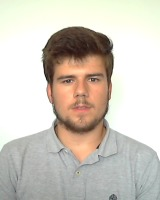
\includegraphics[width=0.25\columnwidth]{figures/sousa.jpg}} &
\textbf{Ricardo B. Sousa} obtained a Master of Science (M.Sc.) degree in Electric and Computers Engineering (ECE) at Faculty of Engineering of the University of Porto (FEUP), in 2020.
He is currently working towards the Ph.D. degree in electrical and computer engineering with FEUP, and he has a graduate research scholarship from FCT -- Fundação para a Ciência e a Tecnologia at the Centre for Robotics in Industry and Intelligent Systems from INESC TEC.
Also, he is an invited assistant lecturing the courses Software Design and Industrial Informatics from the M.Sc. in ECE at FEUP.
His research interests include robotics, sensor fusion, and localization and mapping for autonomous robots.\\
\end{tabular}

%\hfill\break
\newpage

\begin{tabular}{p{0.25\columnwidth} p{0.68\columnwidth}}
\raisebox{-0.925\totalheight}{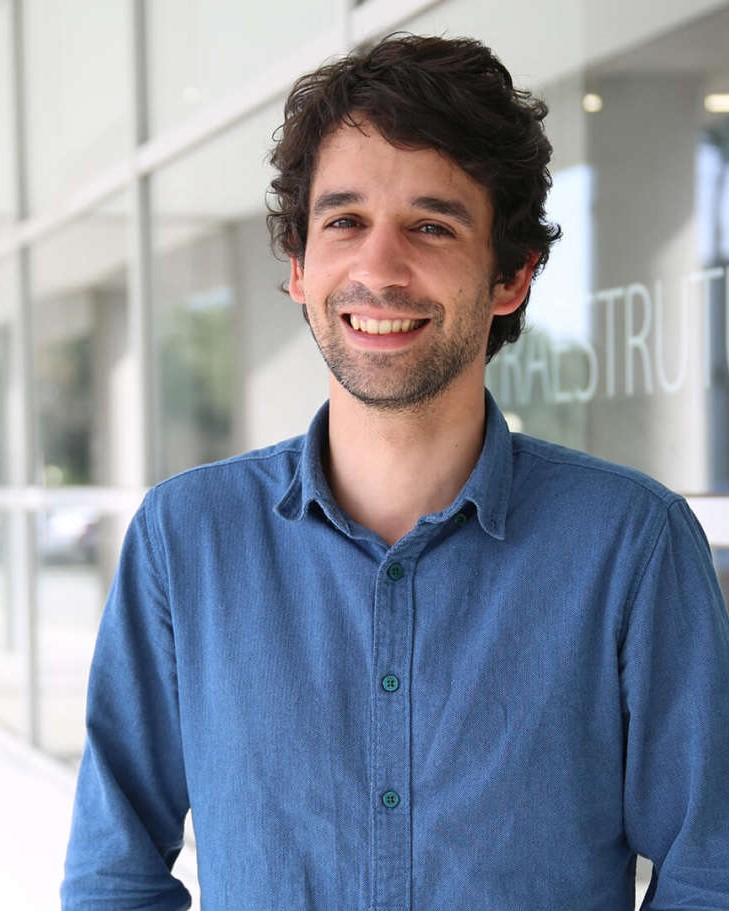
\includegraphics[width=0.25\columnwidth]{figures/sobreira.jpg}} &
\textbf{H\'{e}ber M. Sobreira} was born in Leiria, Portugal, in July 1985. He graduated with an M.Sc. degree (2009) and a Ph.D. degree (2017) in Electrical Engineering from the University of Porto. Since 2009, he has been developing his research within the Centre for Robotics in Industry and Intelligent Systems at INESC TEC. His main research areas are navigation and control of indoor autonomous vehicles.\\
\end{tabular}

%\hfill\break
%\newpage

\begin{tabular}{p{0.25\columnwidth} p{0.68\columnwidth}}
\raisebox{-0.925\totalheight}{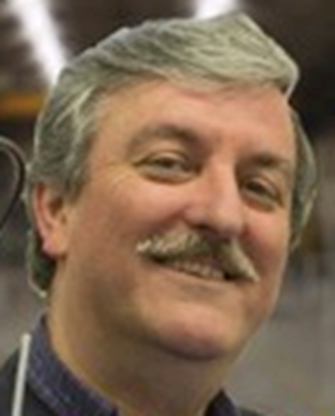
\includegraphics[width=0.25\columnwidth]{figures/moreira.png}} &
\textbf{Ant\'{o}nio Paulo Moreira} graduated with a degree in electrical engineering at the University of Oporto, in 1986. Then, he pursued graduate studies at University of Porto, obtaining a M.Sc. degree in electrical engineering -- systems in 1991 and a Ph.D. degree in electrical engineering in 1998. Presently, he is Associate Professor with tenure at the Faculty of Engineering of the University of Porto and researcher and head of the Centre for Robotics in Industry and Intelligent Systems at INESC TEC. His main research interests are process control and robotics.\\
\end{tabular}



%% APPENDIXES

\cleardoublepage

\section{Introduction}
\label{sec:intro}

An autonomous mobile robot requires a representation of its surroundings to localize itself relative to the environment.
Simultaneous Localization and Mapping (SLAM) addresses this problem by incorporating the robot state estimation (pose and possibly other state variables) concurrently with the mapping process. This process builds a representation of the environment perceived by the robot originating a map incrementally built when exploring unknown areas or refined on passages through known locations.

In a static scene, the robot would only need to map once because it would be always consistent with the environment.
However, autonomous systems deployed in industrial locations, outdoor environments, or even service-oriented applications such as shopping centers or homes deal with moving elements in the scene (humans, objects), environment reconfiguration (machines moving places), and appearance variations (lighting, weather, seasonal, or daytime changes).
These varying conditions are a challenge for the SLAM system, where the system should decide how (consider the most current state or only the most static changes?) and when to update the map (when the variations occur or after a certain time?).
This challenge is also known as the stability-plasticity dilemma, where the long-term localization and mapping should both adapt to new environment changes and preserve old states over time~\parencite{biber-duckett:2009:0278364908096286}.

Furthermore, the map would grow indefinitely when gathering new information from the environment. This ever-growing problem poses another challenge for the SLAM system in the long-term due to the limited computational resources of the mapping vehicle. Indeed, the map size should be dependent on the environment area and not on the trajectory length of the mapping process nor operation time, only growing when the robot would explore unknown locations~\parencite{kretzschmar-stachniss:2012:0278364912455072}.

Although several studies overview SLAM literature, only a subset of those studies mentions long-term challenges of performing SLAM.
\cite{purpose:study:cadena:2016} has a brief survey on the robustness and scalability of autonomous systems focused on loop closure validation, dynamic environments, pose graph sparsification, and parallel and distributed computing for metric and semantic SLAM.
In contrast, \cite{purpose:study:lowry:2016} limits the study to vision-based topological SLAM discussing also the challenge of varying conditions.
While \cite{purpose:study:bresson:2017} overviews autonomous driving trends in terms of scalability, map updatability, and dynamicity, the survey limits the discussion to algorithms that have both odometry and mapping modules, excluding localization-only works. Also, \cite{purpose:study:bresson:2017} focuses more on the modules of the SLAM (relocalization, localization against a map).
\cite{purpose:study:kunze:2018} gives a brief overview of Artificial Intelligence (AI) -related works for robustness to appearance changes and learning dynamics of the environment, discussing areas in which AI enables long-term operation of autonomous systems.
As for \cite{purpose:study:zaffar:2018}, the study evaluates the long-term autonomy of sensors such as monocular and stereo cameras, and LiDAR.
However, to the best of the authors knowledge, none of the existing studies overviews the trends for dealing with long-term challenges in SLAM. Also, the studies that overview some of the challenges of lifelong SLAM do not clarify the process for identifying the cited works, not allowing other researchers to repeat the identification process of records when searching in bibliographic databases.

Therefore, this paper presents a systematic literature review on long-term localization and mapping following the Preferred Reporting Items for Systematic reviews and Meta-Analysis~(PRISMA)~\parencite{methodology:prisma} statement.
The systematic method followed in this review allows the replication of the results by other researchers and leads to the inclusion of 142 works for discussion and analysis.
Also, this paper makes available a public GitHub repository\footnote{\url{https://github.com/sousarbarb/slr-ltlm-mr}} with all the documentation and scripts used during the process of systematic revision of the literature.
The main contributions of this paper relative to the existing studies on SLAM are the following ones:

\begin{itemize}[nosep]
\item discussion on methodologies and trends focused on appearance invariance, dynamic elements, map sparsification and multi-session techniques, and other computational concerns;
\item comparative analysis on the public datasets and experimental data used in the included works in terms of environment conditions, sensorization, and distance and time properties;
\item presentation of common evaluation metrics used by the included works in the experimental results.
\end{itemize}

This review does not intend to review the fundamentals of SLAM nor the main formulations. The reader should refer to \cite{purpose:study:durrant-whyte-bailey:2006:1} and \cite{purpose:study:durrant-whyte-bailey:2006:2} for the Extended Kalman Filter (EKF) and particle filter probabilistic formulations, and to \cite{purpose:study:grisetti:2010} for the pose graph formulation of SLAM.





\subsection{Paper organization}

The rest of this review is organized as follows.
Section~\ref{sec:purpose} discusses the limitations of existent studies and reviews and presents the purpose and motivations of this paper.
Section~\ref{sec:methodology} explains the methodology followed in this review to search and select the included records, and the data extraction process for synthesis and analysis. In Appendix~\ref{a2:data-extraction}, Table~\ref{tab:a2:data-extraction} presents the data extraction results of the included records.
Next, Section~\ref{sec:overview} analyzes the bibliographic information of the 142 included works in this review in terms of the identification results of each data source considered in the methodology, keywords co-occurrence and co-authorship relations, the year of publication, and the publication venue.
Section~\ref{sec:discussion} discusses the methodologies found in the included records related to long-term localization and mapping and analyzes the experimental data and evaluation metrics used in the experiments by the authors.
Then, Section~\ref{sec:future} outlines challenges and future directions.
Section~\ref{sec:limitations} discusses possible limitations of this study.
Lastly, Section~\ref{sec:conclusions} presents the conclusions.

\section{Purpose of the study}
\label{sec:purpose}

\subsection{Limitations of current studies}

\begin{table}[h]
  \renewcommand{\arraystretch}{1.2}
  \setlength{\tabcolsep}{1.75pt}
  \caption[Existent Literature Reviews, Surveys, and Tutorials on SLAM.]{Existent Literature Reviews, Surveys, and Tutorials on SLAM.}
  \label{tab:purpose:current-literature}
  \centering
  {\scriptsize
  \begin{tabular}{p{0.595\columnwidth} p{0.395\columnwidth}}

\hline
\textbf{Topic} & \textbf{Reference}\\
\hline
Probabilistic approaches and data association%
& \cite{background:slam:durrant-whyte-bailey,background:slam:bailey-durrant-whyte}\\
SLAM back end%
& \cite{background:slam:grisetti}\\
Multi-robot SLAM%
& \cite{review:saeedi:2016}\\
Visual odometry%
& \cite{background:slam:scaramuzza-fraundorfer,background:slam:fraundorfer-scaramuzza}\\
Overview of challenges in SLAM%
& \cite{review:cadena:2016}\\
Trends in SLAM for autonomous vehicles%
& \cite{review:bresson:2017}\\
\textbf{Completar tabela!}\\
\hline

  \end{tabular}}
\end{table}

\subsection{Motivations and goals}

Research question: What is the current state of the art of long-term localization and mapping using mobile robots?

Goals of this review:

\begin{itemize}[nosep]
\item which are the main strategies for accomplishing long-term operations with mobile robots;
\item how to deal with varying conditions of the environment;
\item how do autonomous robots deal with the dynamics of the environment;
\item which are the main strategies to deal with the limited computational resources of a mobile robot on long-term operations.
\end{itemize}

PICO framework (Population--Intervention--Comparison--Outcome) helps to frame the research questions of this systematic review into a more structured framework:

\begin{itemize}[nosep]
\item \textbf{Population:} mobile robots;
\item \textbf{Intervention:} localization, mapping, SLAM;
\item \textbf{Comparison:} \textit{not applicable to this study};
\item \textbf{Outcome:} long-term operation, lifelong autonomy, robust.
%\item \textbf{Context:} continuous operation, service robots, industrial environments.
\end{itemize}


\section{Methodology}
\label{sec:methodology}

A systematic literature review uses explicit, rigorous, and reproducible systematic methods to synthesize the findings of studies related to a particular research question, topic area, or phenomenon of interest. This type of review assures the quality and trustworthiness of the review's findings by presenting a complete, organized, and summarized analysis of all works considered while allowing others to replicate or update the reviews. The most common standard for performing a systematic review is the Preferred Reporting Items for Systematic reviews and Meta-Analysis~(PRISMA)~\parencite{methodology:prisma} statement. Although the PRISMA statement has been designed originally for evaluating the effects of health interventions, the checklist items of the methodology are general and applicable to other subject areas. Thus, the methodology used in this systematic review follows the PRISMA~\parencite{methodology:prisma} guidelines.

This section presents the detailed methodology used in this study. First, the eligibility criteria decide which studies to include in the review. Next, the search strategy details the information sources considered in the review and the base string and search fields used for inquiring these sources. Furthermore, the selection process focuses on describing its stages and the quality evaluation criteria used to select works for the synthesis and analysis phase of the review. Lastly, the data extraction process details the relevant data collected for synthesis and analysis.
Parsifal \parencite{methodology:parsifal} is the online tool used to support the literature review in designing the methodology protocol, removing duplicates, screening and selecting works including their quality assessment. Additional documentation and scripts developed within the scope of this review related to removing duplicates, checking and processing the bibliographic references, and data extraction are available in a public GitHub repository\footnote{\url{https://github.com/sousarbarb/slr-ltlm-mr}}.

\subsection{Eligibility criteria}
\label{sec:methodology:eligible}

Table~\ref{tab:methodology:exclusion-criteria} presents the exclusion criteria used to determine the eligible studies for the selection process. These eligibility criteria focus mainly on the type of paper and availability. The index criterion rejects all publications not indexed in a scientific publication venue. This rejection guarantees that the eligible works were peer-reviewed by the scientific community. Also, the exclusion criteria reject short papers and gray, secondary, and tertiary literature. Short papers do not usually present a detailed methodology of their scientific contribution. As for only considering primary literature in the review, this criterion increases the relevance of search results by favoring original articles and simultaneously guaranteeing peer-revision of the works. In terms of language, only considering studies with English full-texts increases the scope and visibility of the review. Similarly, the eligibility criteria reject studies not available in digital libraries for reproducibility and accessibility reasons.

\begin{table}[h]
  \renewcommand{\arraystretch}{1.25}
  \setlength{\tabcolsep}{3pt}
  \caption[Exclusion criteria for the selection process.]{Exclusion criteria for the selection process.}
  \label{tab:methodology:exclusion-criteria}
  \centering
  {\scriptsize
  \begin{tabular}{c m{0.28\columnwidth} m{0.6\columnwidth}}

\hline
\textbf{E\#} & \textbf{Criteria} & \textbf{Statement}\\
\hline
E1 &
Index &
Papers not indexed in a scientific publication venue\\
\hline
E2 &
Language &
Full-text of the papers not published in English\\
\hline
E3 &
Subject Area &
Papers not classified in the databases as Computer Science, Engineering, Mathematics, or Multidisciplinary\\
\hline
E4 &
Short Papers &
Papers classified as short papers accordingly to the publication venue\\
\hline
E5 &
Gray, Secondary, and Tertiary Literature &
Books, preprints, reports, reviews, thesis, ...\\
\hline
E6 &
Availability &
Full-text of the papers not available in digital libraries\\
\hline
E7 &
Dataset &
Papers that focus only on data collection\\
\hline
E8 &
Coverage &
Papers using only odometry for localization\\
\hline
E9 &
Scope &
Papers that focus on different and not related subjects\\
\hline

  \end{tabular}}
\end{table}

Another exclusion criterion considered in the review is relative to the studies' categorization of their subject areas by bibliographic databases. The ones considered in the review are Computer Science, Engineering, Mathematics, or Multidisciplinary areas. In the list provided by the Clarivate's Journal Citation Reports\footnote{\url{https://jcr.clarivate.com/jcr/browse-categories}}, these four subject areas include the artificial intelligence, interdisciplinary applications, electrical and computers engineering, robotics, and applied mathematics categories, among others. These categories are intrinsically related to the localization and mapping problem for long-term operation of mobile robots.

The final three criteria presented in Table~\ref{tab:methodology:exclusion-criteria} focus on the scientific contribution of the studies. The dataset criterion rejects all works that focus only on sharing a data collection. Although these works are important for the evolution of localization and mapping algorithms in providing a benchmark for comparison and reference purposes, their scientific contribution is not directly comparable to research articles. Odometry-only approaches are unusable over long distances invalidating their use for long-term operations with mobile robots. As for the scope criterion, this review does not consider eligible for selection papers not related to long-term localization and mapping.

\subsection{Search strategy}
\label{sec:methodology:search}

The search phase consists of identifying the data sources that could be relevant for this literature review, and defining the base string and which search fields considered to obtain the results for the review. \citetitle{methodology:search:db:wos} and \citetitle{methodology:search:db:scopus} are traditionally the two most widely used bibliographic databases. However, previous studies demonstrate that different databases differ significantly in their scientific coverage~\parencite{methodology:search:db:coverage:scopus-wos,methodology:search:db:coverage:dim-scopus-wos}. Thus, the data sources considered in this review are the following ones: \citetitle{methodology:search:db:acm}, \citetitle{methodology:search:db:dimensions}, \citetitle{methodology:search:db:ieee-xplore}, \citetitle{methodology:search:db:inspec}, \citetitle{methodology:search:db:scopus}, and \citetitle{methodology:search:db:wos}.

Moreover, May 17, 2022, is the date of the last full inquiry. Future reviews on the topic of this study should consider this final date as theirs initial one. As for inquiring the data sources, the base string used is the following one:

\vspace{1em}

\noindent\begin{center}
\begin{tabular}{l l}
\texttt{(robot* OR vehicle*)}                     & \texttt{AND}\\
\texttt{((locali* AND map*) OR "slam")}           & \texttt{AND}\\
\texttt{("long term" OR "life long" OR lifelong)}\\
\end{tabular}
\end{center}

\vspace{1em}

The first terms, \texttt{robot* OR vehicle*}, attempt to focus the search results to the desired population. These two terms have multiple synonyms within the scope of autonomous mobile robots: mobile robots, autonomous vehicles, robotics, agricultural robots, intelligent robots, service robots, unmanned aerial/ground/underwater vehicles, among other terms. Therefore, by adding the asterisk to the end of the terms robot and vehicle (\texttt{robot*} and \texttt{vehicle*}, respectively), and by only considering the terms with asterisk in the inquiry, all the synonyms are covered for the desired population. Given the incompatibility of the \citetitle{methodology:search:db:dimensions} database with wildcards (e.g., using the asterisk), the first part of the base string becomes as follows when searching in this database: \texttt{robot OR robots OR robotics OR vehicle OR vehicles}.

The next part of the query focus on the intervention side of the systematic review. Given the interest of this review on searching for localization and mapping algorithms, \texttt{locali*} and \texttt{map*} summarize all the synonyms for the localization and mapping terms, respectively. For example, \texttt{locali*} not only is agnostic to the US versus UK spelling differences (localization vs localisation, respectively) but also resumes several synonyms: localization, localize, or localizing. The term \texttt{map*} also attempts to cover its respective synonyms such as map, maps, or mapping.
Also, the acronym \texttt{"slam"} is another alternative to search for localization and mapping algorithms. Even though its definition is compatible with \texttt{locali* AND map*}, some authors only refer to SLAM.
Similarly to the inquiry's first part, the second one becomes as follows for searching in \citetitle{methodology:search:db:dimensions}: \texttt{((localize OR localization OR localizing OR localise OR localisation OR localising) AND (map OR maps OR mapping)) OR "slam"}.

As for \texttt{"long term" OR "life long" OR lifelong}, this part of the base string is relative to the outcome of the PICO framework, presented in Section~\ref{sec:purpose}. The reason for having both \texttt{"life long"} and \texttt{lifelong} terms is the existing confusion in which term is grammatically the correct one.

Furthermore, the Title, Abstract, and Keywords are the fields considered for obtaining the search results. The third one includes the author keywords, the indexed terms by the databases, and the uncontrolled ones if they are available. The selection of these search fields for this review improves the relevance of the results compared to using all fields and the full text by focusing the search on the summary items of the works. Indeed, the main contributions of scientific works should be summarized in at least the title, abstract, or the author keywords. The indexed terms also help in obtaining records only related to the base string used in this review.
However, not all data sources have available the search fields considered in the review or some of them require an adaptation when performing the search. 
Although the \citetitle{methodology:search:db:acm} allows searching within multiple search fields, including the ones considered in this review, the advanced search query on this library sets by default an AND operator between the different fields. This setting must be changed manually in the query syntax to the desired OR operator. Also, there are two options to search items in the \citetitle{methodology:search:db:acm}: \textit{The ACM Full-Text Collection} and \textit{The ACM Guide to Computing Literature}. Given that the latter includes all the content from the former, the identification process in this source performs the search using \textit{The ACM Guide to Computing Literature} option.
Other than searching in the publications' full data, \citetitle{methodology:search:db:dimensions} only has the title and abstract search fields compatible with this review. Given the limitation of \citetitle{methodology:search:db:ieee-xplore} to 7 wildcards, the search results of this digital library using the base string for the inquiry are the grouping of different searches considering only a search field at a time, importing each search results to Parsifal and removing the duplicates. As for \citetitle{methodology:search:db:inspec}, \citetitle{methodology:search:db:scopus}, and \citetitle{methodology:search:db:wos}, these databases have available all the search fields considered in the review.

In terms of the publication date, this review does not restrict it to avoid ignoring important works and to improve the discussion. Indeed, to best of the authors knowledge, there is not available a systematic review on long-term localization and mapping for mobile robots to provide an initial date for rejecting older publications. Even though the number of publications per year could indicate an initial date on when the topic gained relevance, the date filtering could still reject important works.

\subsection{Selection process}
\label{sec:methodology:selection}

The selection process of this review summarized in Figure~\ref{fig:methodology:prisma-flow} has three phases: identification, screening, and quality assessment. The first phase consists of inquiring each data source discussed previously with the base string and adapting it if needed. The second phase requires screening the papers. In this review, screening is equivalent to reading the publications' title and abstract and deciding whether the study is eligible or not based on the exclusion criteria. Then, a set of evaluation criteria assesses the quality of the eligible records. The records obtained after the three phases of the selection process are for the data extraction phase.

\begin{figure}[h]
  \centering
  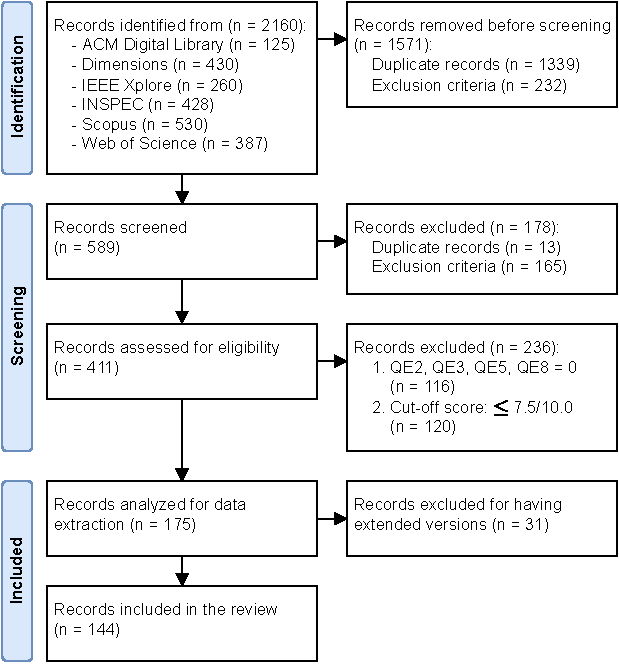
\includegraphics[width=\columnwidth]{figures/selection.pdf}
  \caption{PRISMA flow diagram for the selection process.}
  \label{fig:methodology:prisma-flow}
\end{figure}

\subsubsection{Identification}

In the identification phase of this review, the search strategy is applied to all data sources. \citetitle{methodology:search:db:acm}, \citetitle{methodology:search:db:dimensions}, \citetitle{methodology:search:db:inspec}, \citetitle{methodology:search:db:scopus}, and \citetitle{methodology:search:db:wos} data sources only require a single inquiry to obtain the search results.
Given the limitation of the \citetitle{methodology:search:db:ieee-xplore} for using wildcards mentioned in Section~\ref{sec:methodology:search}, the number of records for this source presented in Figure~\ref{fig:methodology:prisma-flow} represents the results of 7 inquiries (using the fields title, abstract, author keywords, IEEE terms, INSPEC controlled terms, and the INSPEC uncontrolled ones, respectively) after removing the duplicates with the support of Parsifal. Although the total number of search results found is 2160, Parsifal is used to remove duplicates from different data sources, excluding 1339 records. Following the duplicates removal, the exclusion criteria defined in Section~\ref{sec:methodology:search} exclude 232 works from the review. This exclusion is possible due to \citetitle{methodology:search:db:inspec}, \citetitle{methodology:search:db:scopus}, or \citetitle{methodology:search:db:wos} having filters related to the publication's type, subject area, and language.

The works excluded from the search results also include the ones that do not meet the exclusion criteria E4 and E7. For the first one, a Python script available in the GitHub repository of this review searches studies with a number of pages lower or equal to 4. Even though short papers have a maximum number of 3 pages, the papers with 4 pages do not usually present a detailed methodology.
As for the E7 exclusion criterion, some works are possible to remove from the review by searching in their title for the term ``dataset''.
All excluded articles of this review are double-checked to certify if the exclusion criteria are correctly applied. For example, articles published in the Remote Sensing journal from MDPI do not meet the E3 criterion. Indeed, the Journal Citations Reports from Clarivate classifies it by the following categories: Remote Sensing, Geosciences Multidisciplinary, Environmental Sciences, and Imaging Science \& Photographic Technology. However, most search results from this journal found in the identification phase are directly related to the topic of this review and the respective subject areas. Thus, in these cases and in other ones related to the remaining exclusion criteria, the decision is reverted to consider the initially rejected studies for the next phase of the review.

\subsubsection{Screening}

Next, the screening phase in this review consists of reading the title and abstract of the publications and rejecting the ones that meet the exclusion criteria. However, the initially rejected papers have another assessment for validating the exclusion. The analysis of the results and conclusions of these publications considering the exclusion criteria either confirms the exclusion decision or reverses it to eligible works for quality assessment. As a result of the screening phase, 178 studies are rejected from the initial identified 589 works. The duplicate records found in screening and removed manually are due to titles with invalid characters originated by exporting the search results from the \citetitle{methodology:search:db:dimensions}~database.

\subsubsection{Quality assessment}

The quality evaluation in this review of the selected works from screening follows the 8 Quality Evaluation (QE) criteria presented in Table~\ref{tab:methodology:quality-assessment}. All of them are subjective criteria derived from the analysis of the eligible works. The score column establishes the possible values for the QE criteria, in which the minimum, intermediate, and maximum values correspond to none, partial, and full compliance, respectively.
Furthermore, QE1, QE2, QE4, and QE8 focus on the details provided in the papers, specifically, if the discussion of the related work, the proposed methodology, the experimental setup, and the results are detailed and thoroughly analyzed in the publication, respectively.
The possible scores for QE3 are twice the value of QE1, QE2, QE4, and QE8 due to this criterion being directly related to the topic of the review. A work focusing on both localization and mapping problems will have a score of 2.0 (full compliance). If the study only focuses on one of these problems or none of them, the scores will be 1.0 or 0.0, i.e., partial or no compliance, respectively.
QE5 evaluates the long-term results of the eligible studies and is either 2.0 (full) or 0.0 (no compliance). This criterion has the same range as QE3 for similar reasons, given the focus of this review on long-term localization and mapping algorithms.
The definition of long-term experiments for assigning full compliance in QE5 is the following one: dynamic changing environments (e.g., dynamic elements or semi-static ones), increasing environments or feature maps in terms of their size, redundant data removal, or varying conditions (e.g., different seasons of the year or lighting conditions).
QE6 and QE7 can only be 1.0 or 0.0. The former criterion intends to highlight works that compare themselves to the state of the art and/or ground-truth data. The latter emphasizes the importance of having available either the implementation of the proposed methodology or the data used in the experiments for other works to be able to compare the proposed methodologies.
Lastly, considering the possible scores for the QE criteria in Table~\ref{tab:methodology:quality-assessment}, each work can only have a  maximum score of 10.0.

\begin{table}[h]
  \renewcommand{\arraystretch}{1.25}
  \setlength{\tabcolsep}{3pt}
  \caption[Quality evaluation criteria and score range.]{Quality evaluation criteria and score range.}
  \label{tab:methodology:quality-assessment}
  \centering
  {\scriptsize
  \begin{tabular}{c m{0.68\columnwidth} c}

\hline
\textbf{QE\#} & \textbf{Criteria} & \textbf{Score}\\
\hline
QE1 &
Does the paper have an updated state of the art on long-term localization and mapping? &
\{0.0, 0.5, 1.0\}\\
\hline
QE2 &
Is the methodology appropriate and detailed? &
\{0.0, 0.5, 1.0\}\\
\hline
QE3 &
Does the methodology consider both localization and mapping problems? &
\{0.0, 1.0, 2.0\}\\
\hline
QE4 &
Is the hardware and/or software used in the experiments detailed? &
\{0.0, 0.5, 1.0\}\\
\hline
QE5 &
Does the paper presents any kind of long-term experimental results? &
\{0.0, 2.0\}\\
\hline
QE6 &
Does the paper presents comparative results with other methods and/or ground-truth data? &
\{0.0, 1.0\}\\
\hline
QE7 &
Does the work's implementation and/or the data used in the experiments are publicly available? &
\{0.0, 1.0\}\\
\hline
QE8 &
Is the discussion of the results and conclusions appropriate and detailed? &
\{0.0, 0.5, 1.0\}\\
\hline

  \end{tabular}}
\end{table}

After evaluating the 411 eligible works accordingly to the previously discussed QE criteria (the scores of each record are available in the GitHub repository), the first conclusion of the authors is that works with a non-detailed or not appropriate methodology, results' discussion, or conclusions should not be included in the review. Another conclusion is relative to rejecting works that do not consider either localization or mapping problems, or do not present any long-term experimental results, given the focus of this review on the long-term localization and mapping problem for mobile robots. Furthermore, the quality assessment phase should consider a cut-off score to filter works with low quality scores. Consequently, the assessment phase considers the following two reasons to reject a record:

\begin{enumerate}\setlength\itemsep{-0.5em}
\item QE2, QE3, QE5, QE8: reject works with a 0.0 (no compliance) score;
\item cut-off score: reject works with a score lower or equal to 7.5/10.0.
\end{enumerate}

The distribution of the evaluation scores and the QE criteria itself justify the selection of a 7.5/10.0 cut-off score. 
Figure~\ref{fig:methodology:qe} illustrates the scores distribution for all eligible works versus the scores of the ones that pass the first criterion defined previously for the QE phase (related to the compliance on the QE2, QE3, QE5, and QE8 criteria). The assessment of this criterion rejects 116 records (28\%) of the 411 eligible works (see Figure~\ref{fig:methodology:prisma-flow}). 
Even though the distribution of the evaluation scores changes significantly in the range of scores lower or equal to 7.5/10.0, as observed between Figures~\ref{fig:methodology:qe:qe_wo-r1} and~\ref{fig:methodology:qe:qe}, only one work with a score higher than 7.5 is rejected due to not having a detailed and appropriate discussion of the results. This result indicates that interesting works are associated with high scores, as intended when using a quality assessment methodology, while also suggests that the range between 8.0 and 10.0 have the most interesting and quality works compatible with the focus of this review on long-term localization and mapping. Although only assessing the eligible works would seem to lead to the same results in terms of records included in the review, the rejection criterion on QE2/3/5/8 prevents outliers related to the quality assessment.
From the remaining 295 eligible works, cut-off scores from 7.5 up to 8.5 have the following corresponding rejection rates:

\begin{itemize}[nosep]
\item 7.5/10.0 \phantom{$\xrightarrow{\text{reject}}$} 120 records (40.7\%) \phantom{$\xrightarrow{\text{include}}$} 175 records
\item 8.0/10.0 $\xrightarrow{\text{reject}}$ 160 records (54.2\%) $\xrightarrow{\text{include}}$ 135 records
\item 8.5/10.0 \phantom{$\xrightarrow{\text{reject}}$} 203 records (68.8\%) \phantom{$\xrightarrow{\text{include}}$} 92 records
\end{itemize}

\begin{figure}[h]
  \centering
  \subfloat[][]{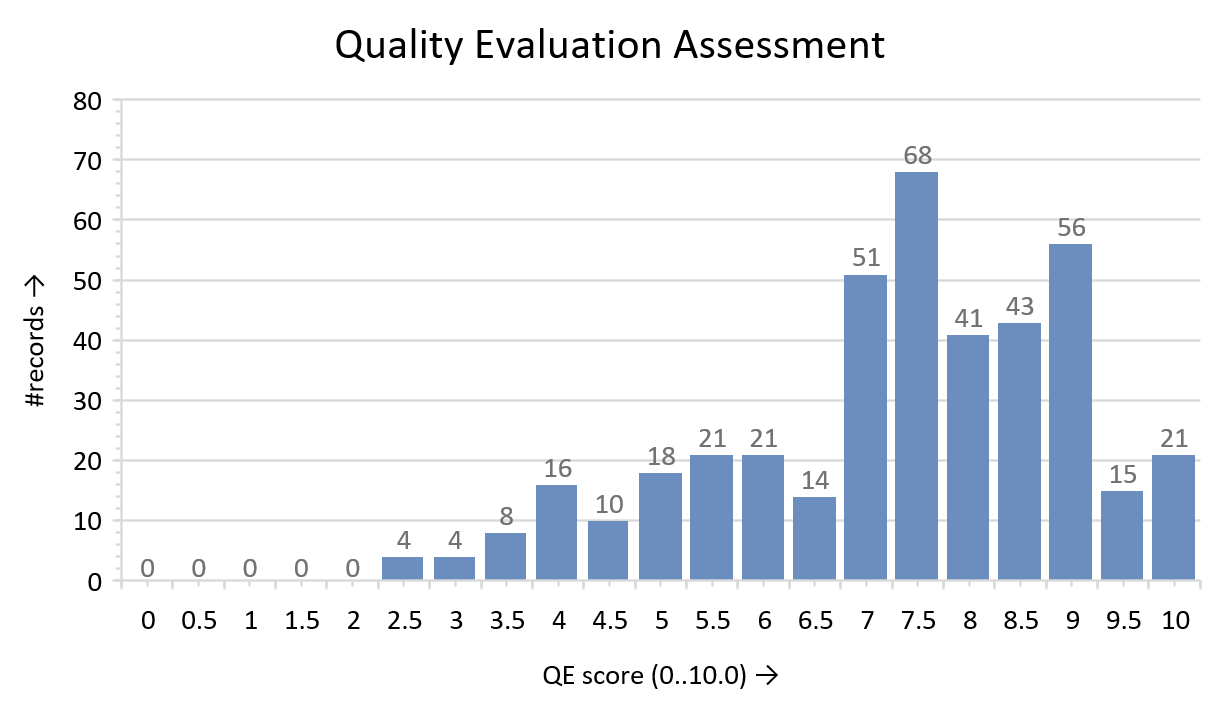
\includegraphics[width=\columnwidth]{figures/qe.png}%
  \label{fig:methodology:qe:qe}}
  \linebreak
  \subfloat[][]{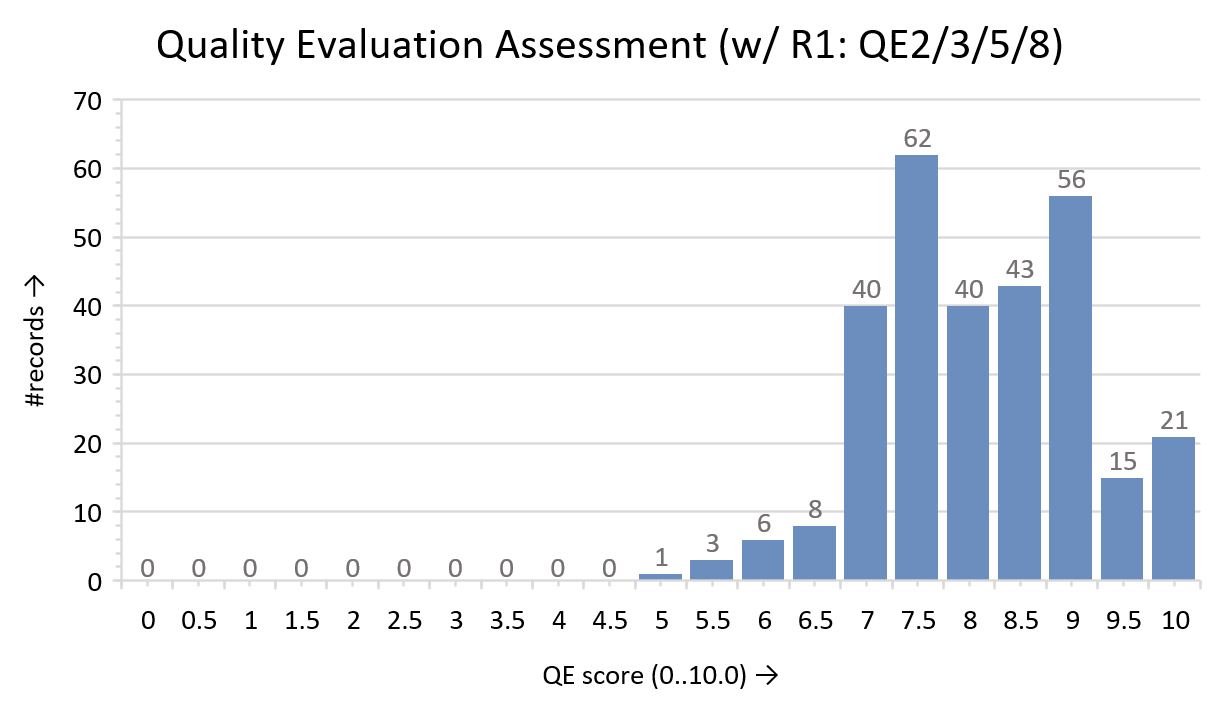
\includegraphics[width=\columnwidth]{figures/qe_wo-r1.png}%
  \label{fig:methodology:qe:qe_wo-r1}}
  \caption{Distribution of the quality evaluation scores obtained from assessing the eligible works considered in the review: (a) all eligible works; (b) works that pass the rejection criterion during the QE assessment related to QE2/3/5/8 = 0.0 (no compliance).}
  \label{fig:methodology:qe}
\end{figure}

The 8.5 cut-off score would not be suitable because methods that focus only on localization or mapping, or not having either the implementation or the experimental data publicly available would be obligated to have maximum scores in the other criteria to be included in the review. In these cases, a work would have a maximum score of 9.0 due to partial compliance on QE3 or no compliance on the QE7 criteria. Likewise, a cut-off score of 8.0 would only leave a margin for having a single partial compliance on QE1, QE2, QE4 or QE8 criteria in similar cases, even though it would reject 160/295 (54\%) records. Therefore, the 7.5/10.0 cut-off score is more appropriate for the quality assessment phase in this review by leaving margin for works to have partial compliance in more than one criterion. Indeed, this cut-off score allows an article with no public data and/or implementation (e.g., due to confidentiality agreements) to have up to four criteria with partial compliance, depending on the criterion's maximum score or if the work has available the experiments data and/or implementation. Another example is articles that only focus on localization or mapping. In these cases, the work could have no public implementation, even though requiring a maximum score on all other criteria, or, if the work has public data or implementation available, two other criteria could have partial compliance.

Overall, as illustrated in Figure~\ref{fig:methodology:prisma-flow}, the quality assessment of the 411 eligible works considering the two rejection criteria previously mentioned leads to rejecting a total of 236 (57\%) records. As a result, the remaining 175 records will be analyzed for data extraction.

\subsection{Data extraction}
\label{sec:methodology:data}

The data extraction process analyzes the records selected after the quality assessment phase and extracts information from these works. In the scope of this review, the Data Extraction (DE) items required for each record are the following ones:

\begin{itemize}[nosep]
\item $\left[\textbf{DE1}\right]$ \textbf{Long-term considerations} -- long-term factors the works consider in their proposed approach and experiments. Considering the knowledge obtained in the previous phases of this review's methodology, the authors considered the following factors for categorizing the included works:
  \begin{itemize}[nosep]
  \item appearance: varying conditions, appearance changes;
  \item dynamics: environment dynamics, dynamic elements;
  \item sparsity: map pruning, redundant data removal;
  \item multi-session: map management;
  \item computational: memory management, efficiency.
  \end{itemize}
\item $\left[\textbf{DE2}\right]$ \textbf{Localization} -- how the robot localizes itself and the type of localizer;
\item $\left[\textbf{DE3}\right]$ \textbf{Mapping} -- type of the map;
\item $\left[\textbf{DE4}\right]$ \textbf{Multi-robot} -- if the proposed methodologies consider multi-robot systems;
\item $\left[\textbf{DE5}\right]$ \textbf{Execution mode} -- offline, online, if requires both, or if no information on this item;
\item $\left[\textbf{DE6}\right]$ \textbf{Environment and domain} -- type of environment (indoor, outdoor) and domains (air, ground, water) tested with the proposed methodologies;
\item $\left[\textbf{DE7}\right]$ \textbf{Sensory setup} -- which sensors considered in the methodologies;
\item $\left[\textbf{DE8}\right]$ \textbf{Non-public experiments} -- if the authors performed experiments or tests with non-public data;
\item $\left[\textbf{DE9}\right]$ \textbf{Ground-truth} -- how ground-truth for non-public data is obtained or its type, if available;
\item $\left[\textbf{DE10}\right]$ \textbf{Distance and time characteristics} -- relative to the non-public experiments if available, as follows:
  \begin{itemize}[nosep]
  \item total distance (km) of the non-public experiments;
  \item path (km), in the case of repetitive paths;
  \item total time (h) in terms of continuous operation;
  \item time interval (day/week/month/year, or d/w/m/y) between the first and the last run.
  \end{itemize}
\item $\left[\textbf{DE11}\right]$ \textbf{Datasets} -- if and which public datasets are used in the experiments;
\item $\left[\textbf{DE12}\right]$ \textbf{Evaluation metrics} -- which metrics are used for evaluation.
\end{itemize}

In Section~\ref{sec:discussion}, a comparison table of the public datasets identified by the DE11 will contain the sensory setup, ground-truth data availability from the datasets, and the distance and time characteristics, similar to the data extraction items for non-public data, among other aspects. As a result, the distinction between public and non-public data availability represented in DE8, DE9, and DE10 allows to understand the distance and time characteristics of non-public data independently from the public datasets.

Although the data extraction phase in a systematic literature review usually does not remove any records, 31 of the analyzed 179 works have extended versions of the proposed methodologies, more detailed ones, or equivalent methods applied in different conditions.
Thus, these records are not included in the review to improve the discussion section in terms of singularity and originality of proposed approaches for the long-term localization and mapping problem.
The extracted information helped identifying the corresponding extended and more complete versions of these works.
A document containing the association of the removed versions to the records included in the review is available in the public GitHub repository, including their bibliographic references. 

Consequently, 144 original works are included in this review for an overview of these records in Section~\ref{sec:overview}, and their synthesis and discussion in Section~\ref{sec:discussion}. The information relative to the 12 data items for each of the included records is available in Appendix~\ref{a2:data-extraction} and also in the repository. The included works represent 35\% of the 411 eligible records for this review. This result indicates that the methodology followed in this review led to a high percentage of quality results.


\section{Results Overview}
\label{sec:overview}

In this section, the main goal is to overview the results not in terms of their scientific contribution but in terms of their bibliographic data for presenting an overview of the included records in the review. First, statistic results of the data sources in which the 142 included records could be identified in the methodology allow the evaluation of the coverage between the sources.
Next, the tool VOSviewer~\parencite{results:vosviewer:1,results:vosviewer:2} is used to obtain the co-occurrence analysis for the keywords and the authors. The former focus on the keywords recency and their occurrence in the sources, while the latter discusses the research networks between the authors, and the ones with more publications in long-term localization and mapping.
Lastly, two analysis are presented relative to the evolution of the publication year and most relevant publication venues.

\subsection{Data source}
\label{sec:overview:db}

The results on the identification phase are exported to BibTeX files from each data source. This exportation considers all the information available in the data sources, such as citation (e.g., author, title, publication venue, and type of record) and bibliographic (e.g., affiliation and the publisher) information of each record, the abstract, and author and indexed keywords. Next, using the \texttt{bibtexparser}\footnote{\url{https://bibtexparser.readthedocs.io/en/master/}} Python library, the BibTeX files are processed to identify uncompleted records. For example, the DOI must be specified and, if not available, the record's information must be manually completed with a corresponding URL. Then, considering the 142 included records in this review, a Python script searches each record in the BibTeX files corresponding to each data source. This search uses the DOI, URL, and title data to identify if a data source had in its identification results the searched record. Given that these three fields can contain lower and upper letters, the respective strings must be compared only after converting them to lower cases. As a result, the number of identified records by each data source of the 142 included ones in the review are the following ones:

\begin{itemize}[nosep]
\item \citetitle{methodology:search:db:acm}: 25 records (17.6\%);
\item \citetitle{methodology:search:db:dimensions}: 84 records (59.2\%);
\item \citetitle{methodology:search:db:ieee-xplore}: 67 records (47.2\%);
\item \citetitle{methodology:search:db:inspec}: 102 records (71.8\%);
\item \citetitle{methodology:search:db:scopus}: 120 records (84.5\%);
\item \citetitle{methodology:search:db:wos}: 105 records (73.9\%).
\end{itemize}

The database \citetitle{methodology:search:db:scopus} is the source that identified the greatest number of included records. This result was expected given that \citetitle{methodology:search:db:scopus} is considered as one of the largest curated databases~\parencite{methodology:search:db:coverage:dim-scopus-wos}, indexing more than 25000 active titles (e.g., conferences proceedings, journals) and 7000 publishers\footnote{\url{https://www.elsevier.com/solutions/scopus/how-scopus-works}}.
Two other sources with more than 70\% of identified records are \citetitle{methodology:search:db:inspec} and \citetitle{methodology:search:db:wos}. Similarly to \citetitle{methodology:search:db:scopus}, these two databases index also records from thousands of journals, conferences, and publishers\footnote{\url{https://www.elsevier.com/solutions/engineering-village/content/inspec}}\textsuperscript{,}\footnote{\url{https://clarivate.com/webofsciencegroup/solutions/web-of-science/}}.
Although \citetitle{methodology:search:db:dimensions} is also a bibliographic database covering millions of publications from thousands of sources, this database is the newest one (created in 2018) relative to the other three considered in this review (\citetitle{methodology:search:db:inspec}, \citetitle{methodology:search:db:scopus}, and \citetitle{methodology:search:db:wos}) and could be a factor to why it obtained a lower percentage (59.2\%) than the other three databases. Another possible reason is that \citetitle{methodology:search:db:scopus} and \citetitle{methodology:search:db:wos} have the majority of their coverage in Life Sciences, Physical Sciences, and Technology Area (including the Engineering subject area related to the topic of this review), while \citetitle{methodology:search:db:dimensions} has better coverage in Social Sciences and Arts \& Humanities~\parencite{methodology:search:db:coverage:dim-scopus-wos}.
Even though \citetitle{methodology:search:db:ieee-xplore} is a digital library and only indexes works published by IEEE and its partners, this data source returns 47.2\% of the include records in the review. The main reason is that this library indexes publications related to electrical engineering and computer science, subject areas related to long-term localization and mapping\footnote{\url{https://ieeexplore.ieee.org/Xplorehelp/overview-of-ieee-xplore/about-ieee-xplore}}.
Finally, the \citetitle{methodology:search:db:acm} using \textit{The ACM Guide to Computing Literature} collection only finds published records by ACM and possible links to other records focused exclusively on computing\footnote{\url{https://libraries.acm.org/digital-library/acm-guide-to-computing-literature}} and not directly related to the Computer Science or Engineering subject areas, explaining why this source obtained a lower coverage percentage of the included results than the other sources for this review.

Furthermore, Table~\ref{tab:overview:source} presents a coverage analysis of the identified results from each data source for the 142 included records in this review. Table~\ref{tab:overview:source:intersect} presents the pairwise overlap between sources. The corresponding percentage is the ratio of records identified by both sources to the one between the two that has the smallest number of results: $\#\{A\cap B\} / \text{min}\{\#A,\#B\}$, where $\#A$ and $\#B$ is the number of results for a data source $A$ and $B$, respectively, and $\#\{A\cap B\}$ is the intersection results between the two sources. For example, if the pairwise results is 100\%, it means that the data source with more records found was capable of obtaining all the results, i.e., had full coverage over the other source. Table~\ref{tab:overview:source:union} reports the percentage of records identified by at least one of two data sources over all 142 included records: $\#\{A\cup B\} / 142$, where $A\cup B$ is the union correspondence results of the sources $A$ and $B$. This percentage represents the joint coverage of two databases over the 142 included records.
					
\begin{table}[h]
  \centering
  \caption{Pairwise coverage analysis of the data sources considered in the review over the 142 included records: (a) identification only on both pairwise sources ($\#\{A\cap B\} / \text{min}\{\#A,\#B\}$); (b) on either ones ($\#\{A\cup B\} / \#\text{records}$). Legend: dim -- \citetitle{methodology:search:db:dimensions}, ieee -- \citetitle{methodology:search:db:ieee-xplore}, insp -- \citetitle{methodology:search:db:inspec}, scop -- \citetitle{methodology:search:db:scopus}, wos -- \citetitle{methodology:search:db:wos}.}
  \label{tab:overview:source}
  \subfloat[][]{%
  \label{tab:overview:source:intersect}%
  \begin{tabular}{l|P{0.08\columnwidth}P{0.08\columnwidth}P{0.08\columnwidth}P{0.08\columnwidth}P{0.08\columnwidth}P{0.08\columnwidth}}
\hline
$A\cap B$ & \textbf{acm} & \textbf{dim} & \textbf{ieee} & \textbf{insp} & \textbf{scop} & \textbf{wos}\\
\hline
\textbf{acm}  & -- & 96.0\% & 44.0\% & 88.0\% & 96.0\% & 96.0\%\\
\textbf{dim}  & -- & --     & 68.7\% & 77.4\% & 97.6\% & 96.4\%\\
\textbf{ieee} & -- & --     & --     & 89.6\% & 91.0\% & 74.6\%\\
\textbf{insp} & -- & --     & --     & --     & 87.3\% & 69.6\%\\
\textbf{scp}  & -- & --     & --     & --     & --     & 89.5\%\\
\textbf{wos}  & -- & --     & --     & --     & --     & --\\
\hline
    \end{tabular}%
  }
  \linebreak
  \subfloat[][]{%
  \label{tab:overview:source:union}%
  \vspace{0.5em}
  \begin{tabular}{l|P{0.08\columnwidth}P{0.08\columnwidth}P{0.08\columnwidth}P{0.08\columnwidth}P{0.08\columnwidth}P{0.08\columnwidth}}
\hline
$A\cup B$ & \textbf{acm} & \textbf{dim} & \textbf{ieee} & \textbf{insp} & \textbf{scop} & \textbf{wos}\\
\hline
\textbf{acm}  & -- & 59.9\% & 57.0\% & 73.9\% & 85.2\% & 74.6\%\\
\textbf{dim}  & -- & --     & 73.9\% & 85.2\% & 85.9\% & 76.1\%\\
\textbf{ieee} & -- & --     & --     & 76.8\% & 88.7\% & 85.9\%\\
\textbf{insp} & -- & --     & --     & --     & 93.7\% & 95.8\%\\
\textbf{scp}  & -- & --     & --     & --     & --     & 92.3\%\\
\textbf{wos}  & -- & --     & --     & --     & --     & --\\
\hline
  \end{tabular}%
  }
\end{table}

Analyzing the coverage results in Table~\ref{tab:overview:source}, the first observation is that the pairwise union results of two sources increase the independent coverage of each source. This observation validates the need identified in the methodology discussed in Section~\ref{sec:methodology} to consider several data sources in the identification phase of a review. Moreover, the pairwise union coverage of \citetitle{methodology:search:db:inspec}, \citetitle{methodology:search:db:scopus}, and \citetitle{methodology:search:db:wos} is greater than 90\% of the included records. When evaluating the joint coverage of these three databases, they identify all 142 of the included records, i.e., a 100\% coverage. Although this result could indicate that those three sources guarantee full coverage of the long-term localization and mapping research topic, it is always advisable to consider as most as possible sources in the methodology. Another observation is relative to the overlap of \citetitle{methodology:search:db:scopus} with the other sources, which is greater than 85\%. This overlap indicates that \citetitle{methodology:search:db:scopus} covers results not only on the topic of this review but also the results obtained by the other sources considered in the methodology. Lastly, \citetitle{methodology:search:db:inspec} and \citetitle{methodology:search:db:wos} achieve a pairwise overlap percentage of 69.6\% between themselves, while their union represents 95.8\% of the included records. This discrepancy indicates that these two sources identify unique results between themselves. Indeed, \citetitle{methodology:search:db:inspec} identifies 31/142 records not found by \citetitle{methodology:search:db:wos}, and vice-versa for \citetitle{methodology:search:db:wos}, with 34/142 unique records.

\subsection{Keywords co-occurrence}
\label{sec:overview:kw}

Next, VOSviewer~\parencite{results:vosviewer:1,results:vosviewer:2} is used to analyze the co-occurrence of keywords in the included articles. This co-occurrence is the relatedness of items determined based on the number of documents in which the keywords occur together.
For this analysis, first, a Python script processes the BibTeX file containing the citation and bibliographic information, the author and the indexed keywords, and the abstract of the records to join the author with the indexed keywords in the same \texttt{keywords} field. Then, an online tool\footnote{\url{https://www.bibtex.com/c/bibtex-to-ris-converter/}} converts this processed BibTeX to a RIS file.
Even though VOSviewer supports file types directly exported from \citetitle{methodology:search:db:dimensions}, \citetitle{methodology:search:db:scopus}, or \citetitle{methodology:search:db:wos} as input, none of these data sources obtained all the 142 included records of the review in the identification phase. Given that VOSviewer does not support BibTeX files, the conversion to RIS file is required for using as input.
The disadvantage of using this file format in VOSviewer is only allowing to perform co-occurrence of items (e.g., keywords or authors), while bibliographic data from \citetitle{methodology:search:db:dimensions}, \citetitle{methodology:search:db:scopus}, or \citetitle{methodology:search:db:wos} in CSV files would allow other analysis such as citation, co-citation, or bibliographic coupling.
However, the creation of these CSV files follow different templates depending on the data source. So, RIS files allow the integration of all 142 included records for obtaining the two co-occurrence analysis presented in this review (namely, keywords and co-authorship).

In Figure~\ref{fig:overview:kw:original}, the network presents the overlay visualization of the keywords co-occurrence in the included records weighted by the number of occurrences of each term, using full counting for the links' strength. The latter computes the strength of the links directly by the number of co-occurrences of the respective two terms.
The overlay visualization colors the keywords differently according to the average publication year of the included records in which each of the keywords appears. This coloring allows analyzing which are the ones that are associated with the most recent publications.
As for the keywords' weighting, the number of occurrences dictates the size of the circles.
Furthermore, the minimum number of occurrences of a keywords set in VOSviewer for obtaining the graph is 5 originating the 34 keywords illustrated in Figure~\ref{fig:overview:kw:original}. This parameter was selected for visualization purposes while also filtering uninteresting keywords.
Similarly, setting the attraction and repulsion parameters to 2 and 0, respectively, distances the terms more from each other than using the values recommended in the VOSviewer manual\footnote{\url{https://www.vosviewer.com/documentation/Manual_VOSviewer_1.6.8.pdf}} (2 and 1, respectively). These two parameters only interfere in the localization of the terms in the map, not in the graph connections.
Lastly, a thesaurus of the keywords (available in the repository) is used to join similar terms: spelling differences (e.g., localization -- localisation), full terms versus abbreviations (simultaneous localization and mapping -- SLAM), while also allowing the concatenation of long keywords for visualization reasons.

\begin{figure*}[!t]
  \centering
  \subfloat[][]{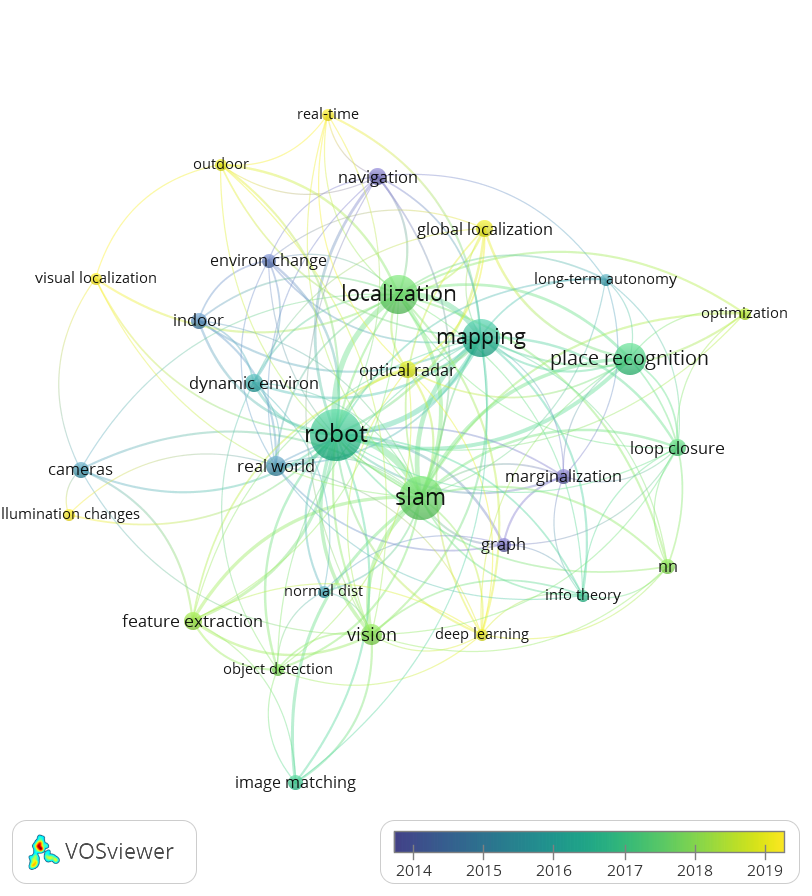
\includegraphics[width=\columnwidth]{figures/kw.png}%
  \label{fig:overview:kw:original}}
  \hfill
  \subfloat[][]{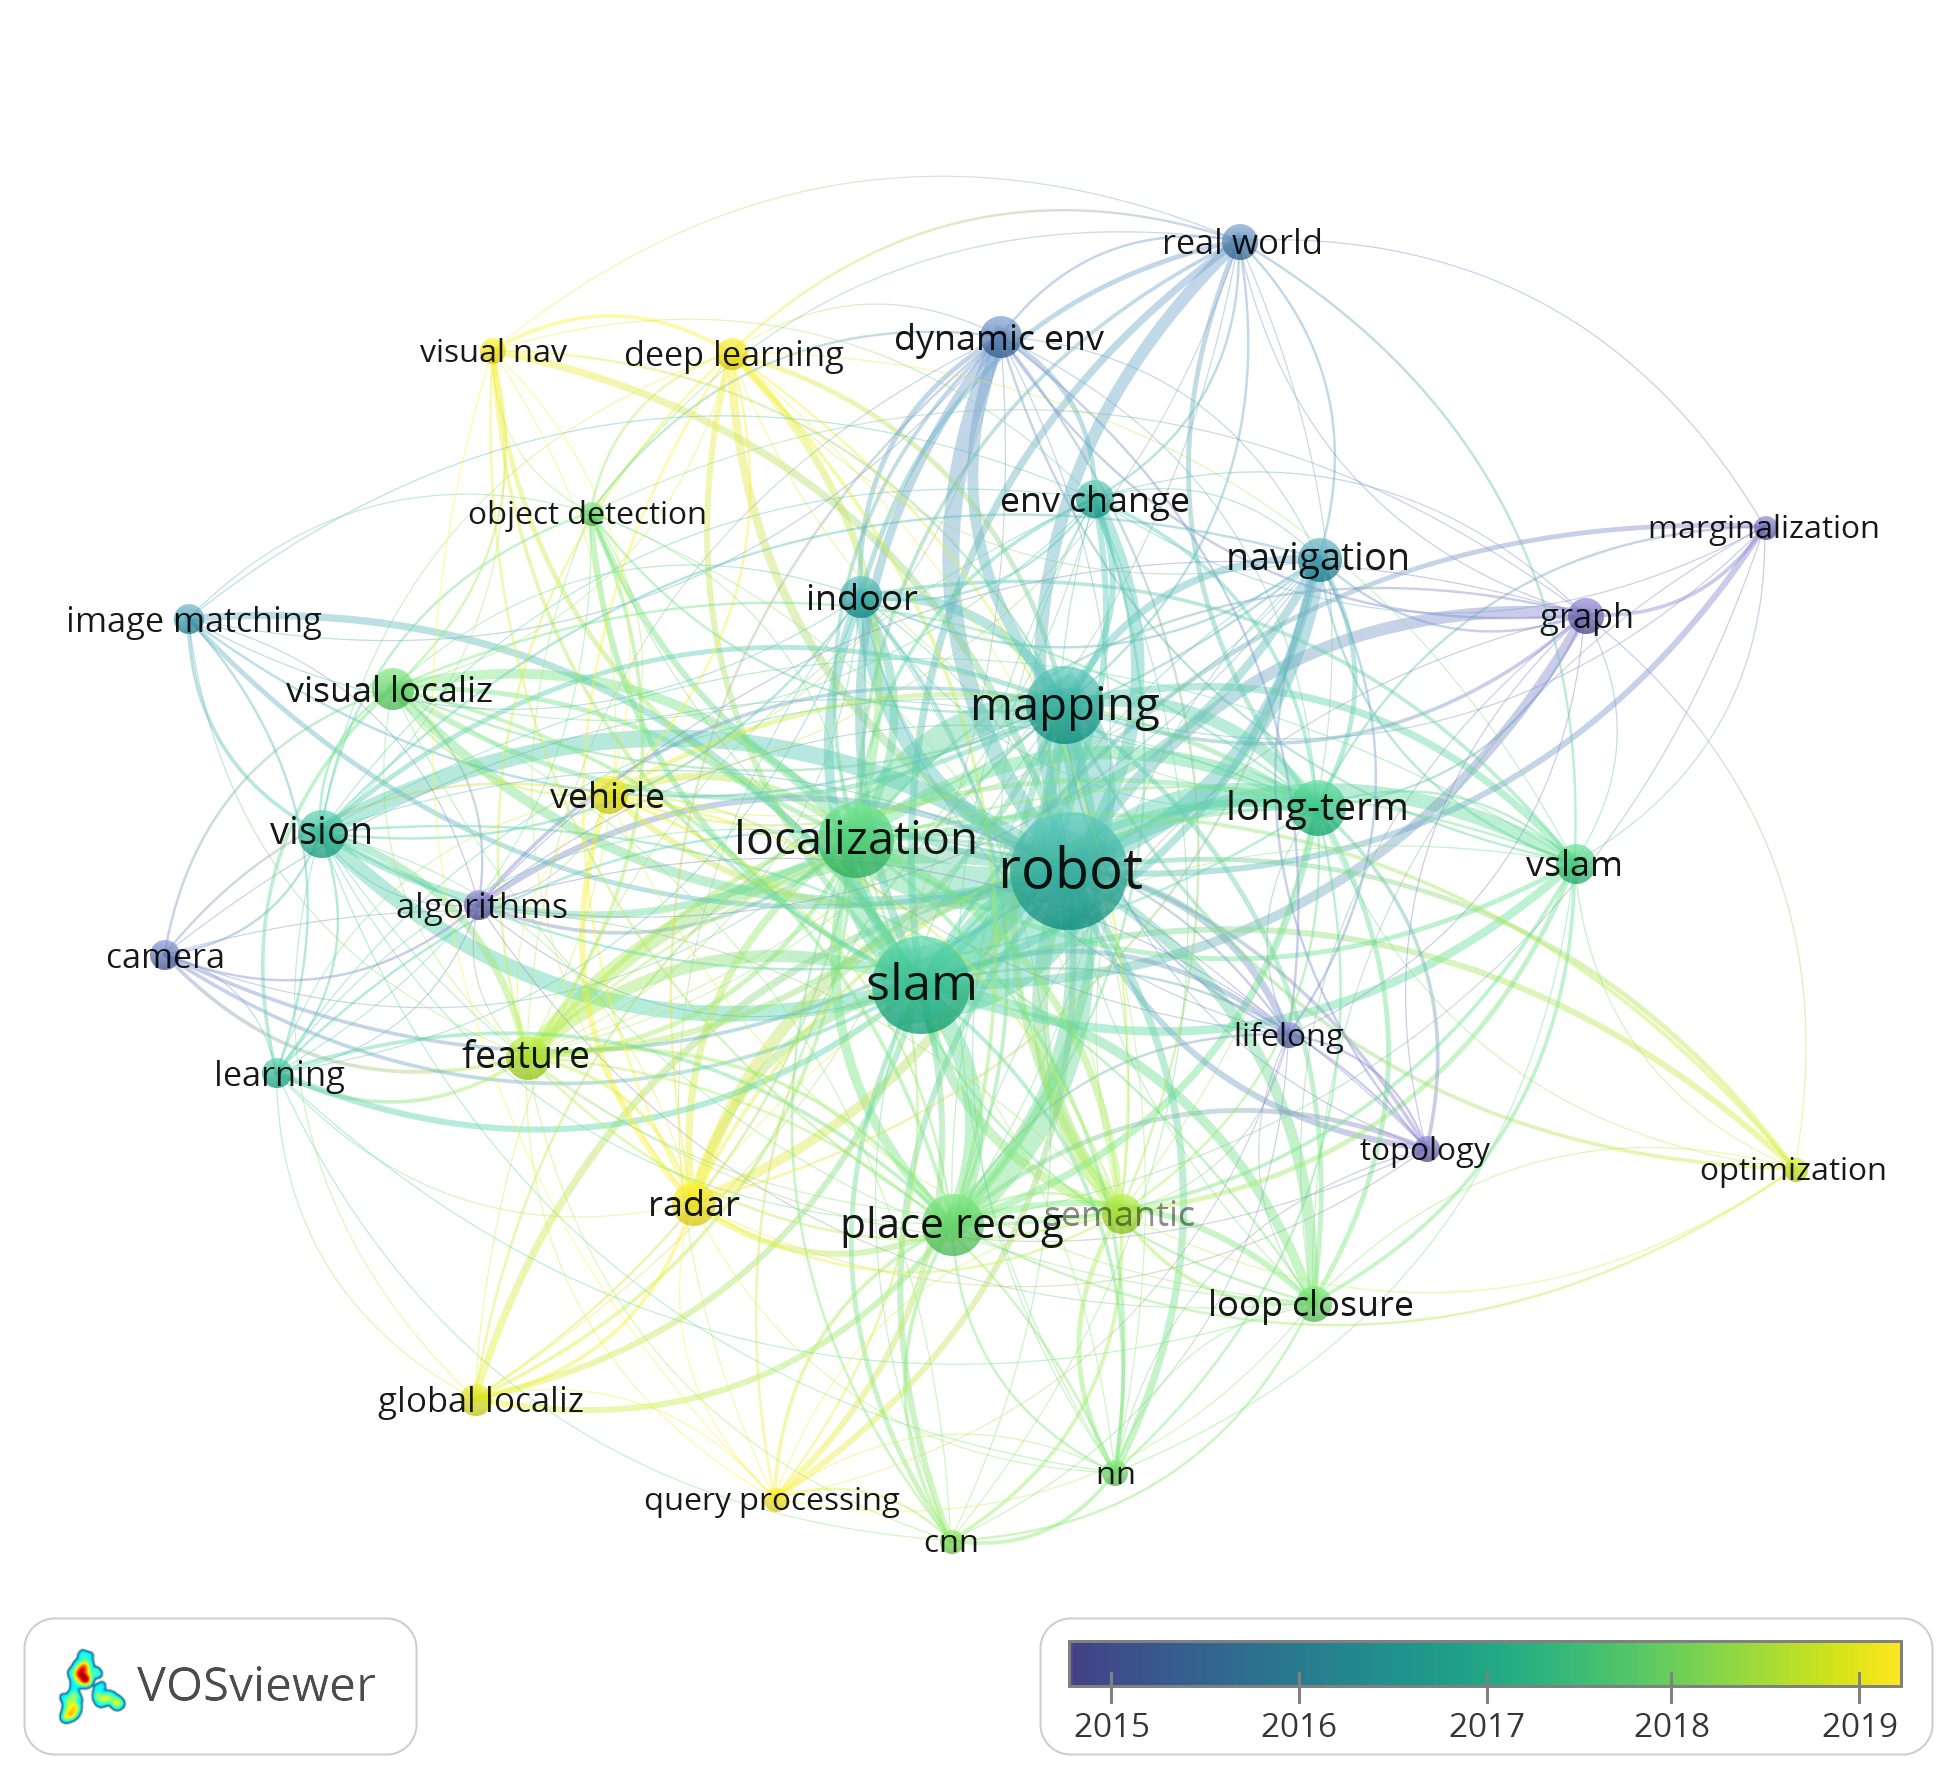
\includegraphics[width=\columnwidth]{figures/kw_long-term.png}%
  \label{fig:overview:kw:long-term}}
  \caption{Keywords co-occurrence analysis on the 142 included records generated by VOSviewer with overlay visualization by the average publication year: (a) original keywords; (b) all keywords containing long-term and lifelong summarized by the terms themselves. Parameters used for generating the co-occurrence network: minimum number of occurrences = 5, attraction = 2, repulsion = 0, scale = 1.49, circles size variation = 0.5, lines size validation = 1.0. Legend: \texttt{cnn} -- Convolutional Neural Networks, \texttt{env} -- environment, \texttt{localiz} -- localization, \texttt{nav} -- navigation, \texttt{nn} -- Neural Networks, \texttt{recog} -- recognition, \texttt{vslam} -- visual SLAM.}
  \label{fig:overview:kw}
\end{figure*}

Overall, the keyword \texttt{robot} is the one that appears more times in the included records: 109 occurrences, links with 33 other terms, and has a total link strength of 390 (sum of co-occurrences of all of its links). This result is expected due to the relation of this review's topic to robotics.
Similarly, three other keywords in the network related to long-term localization and mapping topic with high values of occurrence, number of links, and total link strength are \texttt{slam} (74, 33, and 280), \texttt{mapping} (47, 32, and 196), and \texttt{localization} (46, 31, and 188, respectively). The methodology for the search strategy discussed in Section~\ref{sec:methodology:search} considers all of these four keywords. Thus, the significant influence of \texttt{robot}, \texttt{slam}, \texttt{mapping}, and \texttt{localization} in the keywords co-occurrence analysis indicates that, after the all the phases executed in this review's methodology, the 142 included records have a high correlation with the keywords considered in the search query. Given that the keywords are usually selected or indexed to capture the essence of the document, this correlation indicates that the search query is appropriate to obtain the search results, even considering only the keywords as search fields.

As for keywords related to the outcome of the PICO framework, \texttt{long-term autonomy} occurs only 6 times in the included records, linking with 16 other keywords and having a total link strength of 27. This low occurrence could indicate that the term \texttt{long-term autonomy} is not usually used by the authors nor indexed by the databases. 
However, the specific term of \texttt{long-term autonomy} does not summarize all the possibilities for the outcome of the PICO framework (see Section~\ref{sec:purpose}). Indeed, for this reason, the search query for the identification phase uses only the following single terms: \texttt{"long term"} and \texttt{"life long"} (resumes the possibility of having a space or a hyphen), and \texttt{lifelong}.
Figure~\ref{fig:overview:kw:long-term} presents the keywords co-occurrence analysis using the same parameters for obtaining Figure~\ref{fig:overview:kw:original}. The difference to the latter network is using a thesaurus that summarizes all the keywords that contain \texttt{long-term} and \texttt{lifelong} into the terms themselves, obtaining 35 keywords with a minimum of 5 occurrences in the 142 included records.
In terms of occurrences, number of links, and total link strength, the impact of the thesaurus keyword \texttt{long-term} is 25, 27, and 103, and for lifelong 6, 17, and 31, respectively. These values are much higher than the ones respective only to \texttt{long-term autonomy} from Figure~\ref{fig:overview:kw:original}.
The reason is that \texttt{long-term} in Figure~\ref{fig:overview:kw:long-term} compiles the occurrences of keywords such as \texttt{long-term autonomy}, \texttt{long-term mapping}, and \texttt{long-term localization} (6, 2, and 2 occurrences, respectively), and \texttt{lifelong} sum up, for example, three different versions of \texttt{lifelong learning} (using \texttt{lifelong}, \texttt{life-long} and \texttt{life long} with 2, 1, and 2 occurrences, respectively) and \texttt{lifelong slam} (1 occurrence). Hence, these results proves that the third \texttt{AND} part of the search query (\texttt{"long term" OR "life long" OR lifelong}) covers well the PICO framework's outcome. Plus, they also show no consensus among the authors and by the databases indexation on how to define a keyword for the topic of long-term localization and mapping.

In terms of the average year of publication, analyzing the diagrams in Figure~\ref{fig:overview:kw} on its colorization, the first observation is the recency of terms related to visual localization. The keywords visual SLAM (\texttt{vslam}), visual navigation (\texttt{visual nav}), and visual localization (\texttt{visual localiz}) have all an average publication year higher than 2017. This recency indicates that recent approaches related to the topic of this review, long-term localization and mapping, are more inclined to use vision as a sensorization input.
Another sensor that appeared with high relevance in the network is \texttt{radar}, with 15 occurrences and an average publication year of 2019.20. This sensor is agnostic to the environment changes such as illumination and season changes intrinsically associated with vision and could be the reason why the recent works related to long-term localization and mapping are using it.
Moreover, place recognition (\texttt{place recog}) stands out not only by its recency but importance. The keyword itself (\texttt{place recog}) occurs 31 times and an average publication year of 2017.77, with terms related to place recognition such as \texttt{loop closure} and global localization (\texttt{global localiz}) with recent average publication years (2017.82 and 2018.75, respectively) and strong link to place recognition (5 co-occurrences for each of the links between \texttt{loop closure} and \texttt{global localiz} with \texttt{place recog}). Lastly, machine learning also seems to be used in recent works included in this review. The keywork learning occurs 7 times with an average publication year of 2017.00. Neural Netowrks (\texttt{nn}), Convolutional Neural Networks (\texttt{cnn}), and \texttt{deep learning} have a similar number of occurrences (6, 5, and 8) and publication years higher than 2017 (2017.83, 2018.00, and 2019.12, respectively). These results could mean another trend of using machine learning to improve the long-term autonomy of mobile robots.

Although the recency of keywords related to dynamic environments is lower than 2017 (2015.50 and 2016.75 for \texttt{dynamic env} and \texttt{env change}), they have a high occurrence (14 and 12, respectively), located close to each other in the network, and have a strong link between them (4 co-occurrences). Three keywords also located near each other are \texttt{graph} and \texttt{marginalization} while having similar average publication years (2014.70 and 2014.60, respectively). Even though the number of occurrences of these terms is low (10 and 5 for \texttt{graph} and \texttt{ marginalization}, respectively), their map proximity could indicate a focus in the past on the topic of graph sparsity, i.e., maintaining the graph in the long-term to only depend on the environment size and not on the robot's operation time.

The keywords co-occurrence analysis also relates to the categories of DE1 (see Section~\ref{sec:methodology:data}). Works associated with place recognition, global localization, and loop closure terms require invariance to the appearance changes in the environment, equivalent to the appearance category. The dynamics category is associated with works focused on dynamic environments. As for the other group of keywords with a high occurrence and strong links between each other, the ones related to graph and marginalization, the respective works focus on removing uninformative data from the map~\parencite{kretzschmar-stachniss:2012:0278364912455072}, which is related to map sparsification, and so, to the sparsity category of DE1. These relations between the appearance, dynamics, and sparsity categories to the semantic analysis of the keywords co-occurrence supports the categorization of DE1 considered in this review, while also indicating that the discussion on the proposed methodologies should focus on each one of the categories. Even though the two remaining categories of DE1 (multi-session and computational) are not represented in the keyword analysis, the execution of the data extraction phase identified the need for having these two categories, given the importance of multi-session handling and computational efficiency for long-term localization and mapping. However, each category of DE1 will be discussed in Section~\ref{sec:discussion} in further detail.


\subsection{Co-authorship analysis}
\label{sec:overview:authors}

The other analysis obtained using VOSviewer is the co-authorship network presented in Figure~\ref{fig:overview:authors}. Similar to the keywords network illustrated in Figure~\ref{fig:overview:kw}, the co-occurrence of the authors' names creates links among them in the graph. The strength of these links is dictated by the number of documents the two authors of a link are co-authors in the same record, and the number of co-authored works determines the size of the circles respective to each author in the graph. 
In contrast to Figure~\ref{fig:overview:kw}, the network in Figure~\ref{fig:overview:authors} does not have any overlay specific to coloring depending on the average publication year. Instead, the main goal of the co-authorship analysis in this review is to present possible research networks detected in the 142 included records. Thus, the coloring in Figure~\ref{fig:overview:authors} represents the clusters of authors detected by VOSviewer. This network only considers authors with a minimum of 3 works for relevance and visualization reasons, resulting in 27 authors.
Also, authors identified only by the initial of the first name and by the surname can lead to incorrect correspondences in terms of co-authorship. VOSviewer detects 392 authors in the 142 included records using the original RIS file used in Section~\ref{sec:overview:kw} compared to 413 after checking the authors names. Indeed, a manual check is performed on all authors of the included records to guarantee no false correspondences for the co-authorship analysis with VOSviewer. This manual check ensures each author has its full first and surname and any middle initials while also using the same name for an author in different records.

\begin{figure}[h]
  \centering
  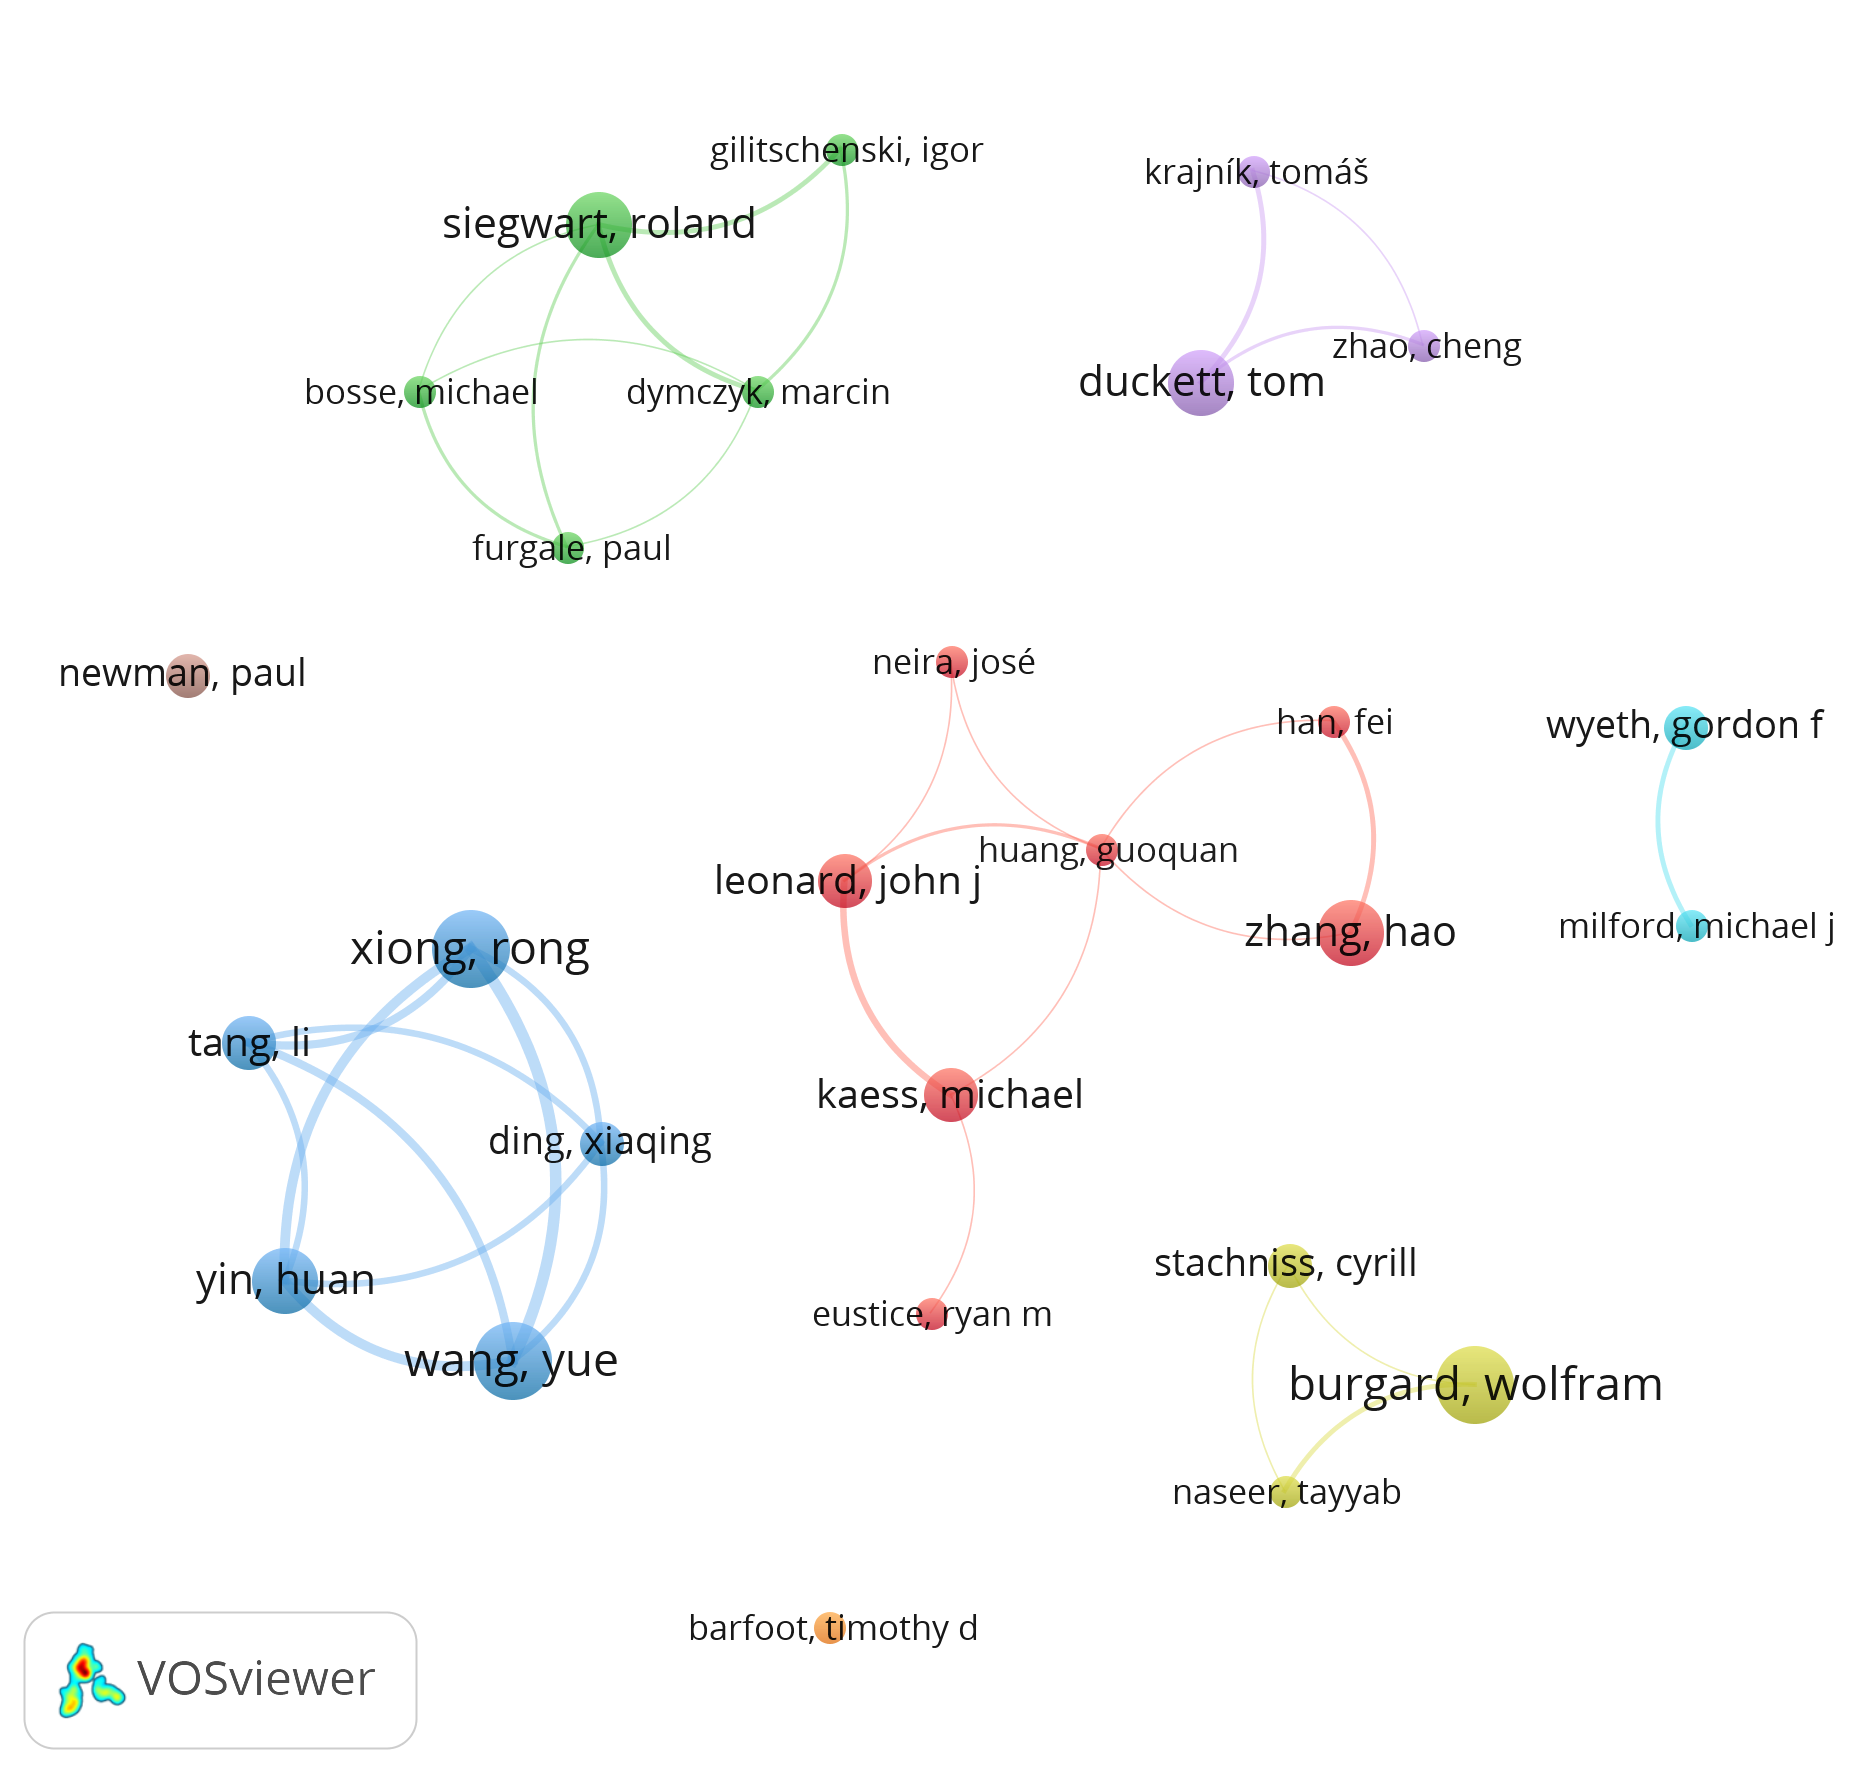
\includegraphics[width=\columnwidth]{figures/authors.png}
  \caption{Co-authorship analysis on the 142 included records generated by VOSviewer. Parameters used for generating the co-occurrence network: minimum number of occurrences = 3, attraction = 4, repulsion = -2, scale = 1.49, circles size variation = 1.0, lines size validation = 1.0.}
  \label{fig:overview:authors}
\end{figure}

Analyzing Figure~\ref{fig:overview:authors}, the co-authorship network presents 8 clusters. These clusters are separated from each other, i.e., no link exists between authors from different clusters. However, this separation does not mean that there is not any co-authorship between authors from different clusters only indicating that for a minimum of 3 co-authored documents there is not a connection between the authors of these 8 clusters. Even so, the graph presented in Figure~\ref{fig:overview:authors} allows the identification of the most relevant research networks in terms of number of co-authored documents and in the context of long-term localization and mapping, considering the 142 records included in this review. As a results, the following enumeration presents the authors that belong to each cluster in the format of author (number of co-authored documents):

\begin{enumerate}\setlength\itemsep{-0.5em}
\item Rong Xiong \orcid{0000-0001-9318-9014}\textsuperscript{,}\scholar{1hI9bqUAAAAJ} (7),
      Yue Wang \orcid{0000-0002-0981-935X}\textsuperscript{,}\scholar{N543LSoAAAAJ} (7),
      Huan Yin \orcid{0000-0002-0872-8202}\textsuperscript{,}\scholar{1fNc3vUAAAAJ} (6),
      Li Tang \orcid{0000-0003-2590-6872} (5), and
      Xiaqing Ding \orcid{0000-0001-7802-0130}\textsuperscript{,}\scholar{6u5OHUcAAAAJ} (4);
\item Hao Zhang \scholar{Ug2VxyUAAAAJ} (6),
      John J. Leonard \orcid{0000-0002-8863-6550}\textsuperscript{,}\scholar{WPe7vWwAAAAJ} (5),
      Michael Kaess \scholar{27eupmsAAAAJ} (5),
      Fei Han \orcid{0000-0002-8619-3987} (3),
      Guoquan Huang \scholar{trMUyZIAAAAJ} (3),
      José Neira \orcid{0000-0003-0668-977X}\textsuperscript{,}\scholar{scoMbR8AAAAJ} (3), and
      Ryan M. Eustice \orcid{0000-0002-9989-4942}\textsuperscript{,}\scholar{WroYmiAAAAAJ} (3);
\item Wolfram Burgard \orcid{0000-0002-5680-6500}\textsuperscript{,}\scholar{zj6FavAAAAAJ} (7),
      Cyrill Stachniss \orcid{0000-0003-1173-6972}\textsuperscript{,}\scholar{8vib2lAAAAAJ} (4), and
      Tayyab Naseer \orcid{0000-0002-3350-3005}\textsuperscript{,}\scholar{1FePZqEAAAAJ} (3);
\item Roland Siegwart \orcid{0000-0002-2760-7983}\textsuperscript{,}\scholar{MDIyLnwAAAAJ} (6),
      Igor Gilitschenski \orcid{0000-0001-6426-365X}\textsuperscript{,}\scholar{Nuw1Y4oAAAAJ} (3),
      Marcin Dymczyk \orcid{0000-0003-3667-8764}\textsuperscript{,}\scholar{XYHy7U8AAAAJ} (3),
      Michael Bosse \scholar{eopb1VgAAAAJ} (3), and
      Paul Furgale \orcid{0000-0002-7367-1046}\textsuperscript{,}\scholar{RNDtSG8AAAAJ} (3);
\item Tom Duckett \orcid{0000-0003-2971-7905}\textsuperscript{,}\scholar{et1GU2EAAAAJ} (6),
      Cheng Zhao \orcid{0000-0001-8502-3233}\textsuperscript{,}\scholar{EAC-8m0AAAAJ} (3), and
      Tomáš Krajník \orcid{0000-0002-4408-7916}\textsuperscript{,}\scholar{Qv3nqgsAAAAJ} (3);
\item Gordon F. Wyeth \orcid{0000-0002-4996-3612}\textsuperscript{,}\scholar{yfXZfXEAAAAJ} (4) and
      Michael J. Milford \orcid{0000-0002-5162-1793}\textsuperscript{,}\scholar{TDSmCKgAAAAJ} (3);
\item Paul Newman \scholar{BtO5fTUAAAAJ} (4);
\item Timothy D. Barfoot \orcid{0000-0003-3899-631X}\textsuperscript{,}\scholar{N_vPIhoAAAAJ} (3).
\end{enumerate}

When analyzing the affiliations of the authors mentioned previously at the time of publication, all authors of the first cluster belonged to the State Key Laboratory of Industrial Control and Technology (SKLICT) and the Institute of Cyber-Systems and Control at Zhejiang University in China. Even though Huan Yin, Yue Wang, Xiaqing Ding, Li Tang, and Rong Xiong mention their affiliation to the Joint Centre for Robotics Research between Zhejiang University, China, and the University of Technology Sydney, Sydney, in the work \cite{yin-et-al:2020:2905046}, this specific affiliation only appeared in this article. The total link strength (sum of all links weights) of each of the authors in that cluster is higher than 16, meaning a high co-authorship between them. Indeed, all five authors have links between all of them.
Similar to the first cluster, the third, fourth, fifth, and sixth clusters have common affiliations within each one: the Autonomous Intelligent Systems at the University of Freiburg in Germany, the Autonomous Systems Lab (ASL) at ETH Zürich in Switzerland, the Lincoln Centre for Autonomous Systems (LCAS) at the University of Lincoln in UK, and the School of Electrical Engineering and Computer Science at Queensland University of Technology (QUT) in Australia, respectively.
However, the interlinking between the authors is not as strong as in the first cluster, as shown in Figure~\ref{fig:overview:authors} by the authors of these clusters not being connected between all the ones within each cluster. Even so, the common affiliation shows there is considerable interest by these research units in the long-term localization and mapping topic.

The affiliation analysis in the second cluster is more complex given that there was no affiliation common to all authors at the time of the records' publication. Instead, the following affiliations were found: Fei Han and Hao Zhang with the Department of Computer Science at Colorado School of Mines in the USA, Guoquan Huang with the Department of Mechanical Engineering at the University of Delaware in the USA, John J. Leonard and Michael Kaess with the Computer Science and Artificial Intelligence Laboratory (CSAIL) at the Massachusetts Institute of Technology (MIT) in the USA, Ryan M. Eustice with the Perceptual Robotics Laboratory (PeRL) at the University of Michigan in the USA, and José Neira with the Instituto Universitario de Investigación en Ingeniería de Aragón (I3A) at the Universidad de Zaragoza in Spain.
Although there are 5 different affiliations to which the 7 authors stated in the respective records, 4 of the research institutions noted for the second cluster are in the USA, indicating a possible reason for facilitating the linkage between these authors from different research units.

In terms of the clusters composed by single authors, the affiliations of Paul Newman and Timothy D. Barfoot are the Oxford Robotics Institute at the University of Oxford in UK and the Autonomous Space Robotics Laboratory (ASRL) at the University of Toronto Institute for Aerospace Studies (UTIAS) in Canada, respectively. Even though these two authors are not linked with any others in the network, the co-authorship analysis indicates that they have an interest in long-term localization and mapping. This interest is shown by their number of co-authored records: 4 and 3 by Paul Newman and Timothy D. Barfoot, respectively.

As for the number of co-authored publications, considering the 142 included records, the authors that appeared to have more research on the review's topic are Rong Xiong, Yue Wang, and Wolfram Burgard, given the 7 co-authored publications of each one. However, Rong Xiong and Yue Wang have co-authored the 7 documents attributed to each of them. This relation and similar ones can biase the analysis of which authors are having more impact in the review's topic.
The clustering shown in Figure~\ref{fig:overview:authors} allows a more unbiased analysis relative to the co-authorship links between authors. Thus, based on the clustering and which author from each cluster has the most co-authored publications, the most influential authors in long-term localization and mapping are the following ones: Rong Xiong (or Yue Wang), Hao Zhang, Wolfram Burgard, Roland Siegwart, Tom Duckett, Gordon F. Wyeth, Paul Newman, and Timothy D. Barfoot.

\subsection{Year of publication}
\label{sec:overview:year}

The relevance of the long-term localization and mapping topic can be evaluated by the evolution of the number of publications. Figure~\ref{fig:overview:year} presents this evolution from the earliest year of publication of the included records to the year at the time of writing this article. The latter has its respective data dashed to indicate that the last year is not completed at the time of writing. Analyzing Figure~\ref{fig:overview:year}, this review's topic seems to have gain relevance in 2009 with 6 works, compared to only one publication in 2007 and another in 2002 in the previous years to 2009. From that year onwards, the graph has an almost linear tendency reaching a maximum of 23 records in 2021, while already having 8 publications in 2022 until May 17, 2022. This tendency shows that long-term localization and mapping is gaining interest throughout the years and, consequently, supports the importance and relevance of this review for the scientific community.

\begin{figure}[!h]
  \centering
  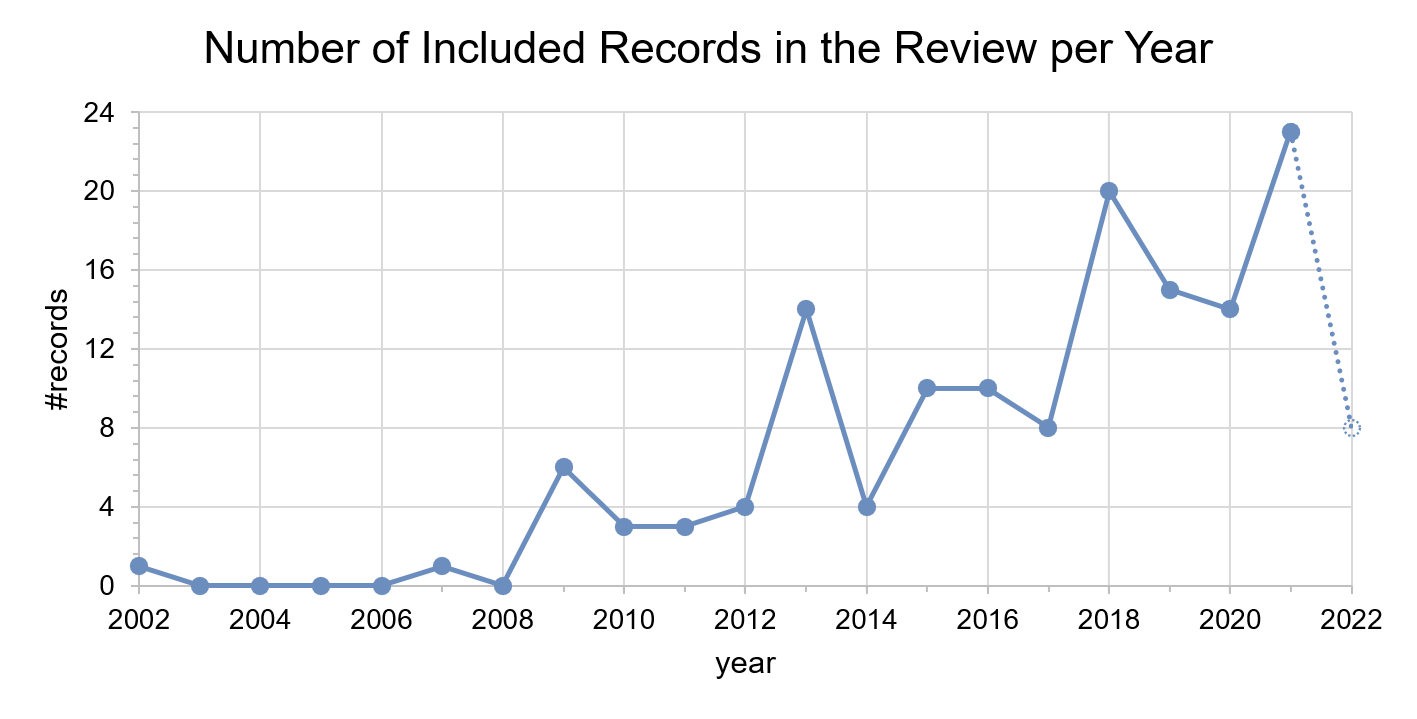
\includegraphics[width=\columnwidth]{figures/year.png}
  \caption{Evolution of published records per year considering the 142 included records in this review.}
  \label{fig:overview:year}
\end{figure}

\subsection{Publication venue}
\label{sec:overview:publication}

Finally, the last overview of the 142 included records in the review is relative to the publication venue. Table~\ref{tab:overview:publication} presents the venues with more than 1 publication, separating the journals and conferences in two different tables (Tables~\ref{tab:overview:publication:journal} and \ref{tab:overview:publication:conference}, respectively).
The columns $\mu$ present the average year of publication of the records associated to a certain venue, while $\text{max}$ columns display the publishing recency by the year of the most recent publication in the venue. For comparing to the average value ($\mu$), the third column ($\sigma$) of each table presents the standard deviation based on the publication year data.
The last column state the number of records published in the venue from the 142 records included in the review for discussion.

\begin{table}[!h]
  \centering
  \caption{Publication venues of the included records in this review with more than one record published in the venue: (a) journals; (b) conferences. Legend: $\mu$ -- average year of publication, $\sigma$ -- standard deviation of the publication year, $\text{max}$ -- maximum year of publication, \# -- number of records published at a certain venue.}
  \label{tab:overview:publication}
  \subfloat[][]{%
  \begin{tabular}{p{0.55\columnwidth}cccc}
\hline
                 & \multicolumn{3}{c}{\textbf{Year}} & \\
\cline{2-4}
\textbf{Journal} & $\mu$ & $\sigma$ & $\text{max}$ & \textbf{\#}\\
\hline
Robotics and Autonomous Systems & 2016 & 3.9 & 2021 & 13\\
IEEE Robotics and Automation Letters & 2019 & 1.7 & 2022 & 12\\
International Journal of Robotics Research & 2014 & 3.2 & 2022 & 11\\
Journal of Field Robotics & 2017 & 3.5 & 2022 & 8\\
Autonomous Robots & 2017 & 2.2 & 2020 & 7\\
IEEE Transactions on Intelligent Transportation Systems & 2021 & 0.8 & 2022 & 4\\
Sensors & 2019 & 0.8 & 2020 & 4\\
IEEE Transactions on Robotics & 2017 & 3.1 & 2022 & 4\\
IEEE Sensors Journal & 2020 & 1.5 & 2021 & 2\\
International Journal of Advanced Robotic Systems & 2020 & 1.5 & 2021 & 2\\
\hline
  \end{tabular}\label{tab:overview:publication:journal}%
  }
  \linebreak
  \subfloat[][]{%
  \begin{tabular}{p{0.55\columnwidth}cccc}
\hline
                    & \multicolumn{3}{c}{\textbf{Year}} & \\
\cline{2-4}
\textbf{Conference} & $\mu$ & $\sigma$ & $\text{max}$ & \textbf{\#}\\
\hline
IEEE International Conference on Robotics and Automation (ICRA) & 2016 & 3.9 & 2021 & 22\\
IEEE/RSJ International Conference on Intelligent Robots and Systems (IROS) & 2017 & 3.6 & 2021 & 17\\
IEEE International Conference on Robotics and Biomimetics (ROBIO) & 2019 & 2.1 & 2021 & 3\\
IEEE International Intelligent Transportation Systems Conference (ITSC) & 2018 & 2.4 & 2021 & 3\\
European Conference on Mobile Robots (ECMR) & 2014 & 0.9 & 2015 & 3\\
IEEE Intelligent Vehicles Symposium (IV) & 2019 & 0.5 & 2019 & 2\\
International Conference on 3D Vision (3DV) & 2018 & 1.5 & 2019 & 2\\
International Conference on Advanced Robotics (ICAR) & 2011 & 2.0 & 2013 & 2\\
\hline
  \end{tabular}\label{tab:overview:publication:conference}%
  }
\end{table}

In terms of journals, the Robotics and Autonomous Systems, IEEE Robotics and Automation Letters, and the International Journal of Robotics stand out with more than 10 publications. Also, these journals have a high standard deviation (greater than 1.5), indicating that the publications spread out throughout the years.
In the case of the IEEE Robotics and Automation Letters, these results gain more relevance indicating a recent trend on publishing on this journal, considering that its creation was only on 2015\footnote{\url{https://www.ieee-ras.org/publications/ra-l}}.
With more than 5 publications, the Journal of Field Robotics and the Autonomous Robots have recent average of publication (2017) with a high standard deviation (greater than 2.0), similarly indicating that authors have been publishing in these two journals along the years.
In contrast, the IEEE Transactions on Intelligent Transportation Systems and Sensors journals have a standard deviation lower than 1 year, with an average publication year of at least 2019. The recency of publication on these two journals with a very low deviation suggests a recent interest of the authors to publish in these two journals works related to long-term localization and mapping.

As for conferences, the data in Table~\ref{tab:overview:publication:conference} shows a high discrepancy in the number of publications related to this review's topic in ICRA and IROS compared to the other venues. Indeed, all the other conferences have only a maximum of 3 records published in them, compared to 22 and 17 papers in ICRA and IROS, respectively. When considering that 60 of the 142 included records are published in conferences, ICRA and IROS with a total of 39 published works related to this review's topic represent 65\% of works published in conferences and 27.5\% of all included records. This result expresses the high relevance of ICRA and IROS in the topic of long-term localization and mapping.


\section{Discussion}
\label{sec:discussion}

The main goal of this review is to synthesize methodologies focused on long-term localization and mapping. Therefore, the discussion first analyzes the techniques proposed in the 142 included works for the five categories of DE1 (see Section~\ref{sec:methodology:data}). Section~\ref{sec:discussion:appearance} discusses methodologies related to dealing with the varying appearance of environments for localization and place recognition. Section~\ref{sec:discussion:dynamics} analyzes works focused on modeling the environment dynamics or identifying dynamic objects within the environment. Section~\ref{sec:discussion:sparsity} focuses on approaches for removing redundant data from the map or identifying novelty data to keep the map size constrained to the environment size. Section~\ref{sec:discussion:multisession} discusses how methods handle multi-session in terms of mapping. Section~\ref{sec:discussion:computational} reviews works related to computation concerns over long-term localization and mapping, in addition to the ones relative to map sparsification discussed in Section~\ref{sec:discussion:sparsity}. However, the discussion should also focus on how the included works evaluated their results in long-term operations. Thus, Section~\ref{sec:discussion:experiments} analyzes the experimental data and datasets used in the experiments, and Section~\ref{sec:discussion:metrics} presents the evaluation metrics used for evaluating the proposed methodologies.





\subsection{Appearance variance}
\label{sec:discussion:appearance}

Next, the discussion focuses on included works categorized in DE1 as appearance. The different methodologies found in these works deal with variable lighting changes, perspective or viewpoint variance, moving elements in the scene, different weather conditions, or changes caused by the year's seasons.
In order to improve the discussion, the analysis of the proposed techniques related with appearance invariance is organized into the following topics: experience maps for treating different appearances as multiples experiences, handcrafted features, features extracted using Convolutional Neural Networks (CNN), assessment of feature stability, multi-modal features, leverage of temporal coherence by image sequence matching, and a discussion of the different sensors modalities used in the included works for appearance invariance.



\subsubsection{Experience maps}
\label{sec:discussion:appearance:exp-maps}

One way to deal with the appearance variance of environments is by treating different conditions as multiple experiences.
The biologically inspired RatSLAM~\parencite{ball-et-al:2013:9} introduces the experience map as a semi-metric topological map, where each experience is a view of the environment at a certain position and wheel odometry provides the relative pose for the links. New experiences are created when none of the previous ones saved in the map are sufficiently similar in appearance to the current scene.
\cite{glover-et-al:2010:5509547} combines the mapping of RatSLAM with the place recognition of FAB-MAP~\parencite{discussion:fab-map}. The latter improves the loop closure detection of the original RatSLAM due to FAB-MAP having light invariant characteristics for data association by learning a generative model for the Bag of Words (BoW) model~\parencite{discussion:bow}.
Both RatSLAM and the hybrid RatSLAM+FAB-MAP systems uses visual data to retrieve information from the environment.
Although \cite{martini-et-al:2020:s20216002} uses also experience-based mapping, the main sensor is a radar, where an experience is represented by a point cloud from the sensor and the point descriptors retrieved from it. Radar is known for being less affected by environment changes such as different illumination or weather conditions compared to vision sensors~\parencite{hong-et-al:2022:02783649221080483}.

The concept of adding the environment changes to the map identified by the degradation in localization is also employed by \cite{konolige-bowman:2009:5354121} and \cite{tang-et-al:2019:7}.
The former implements a keyframe SLAM system created from the Visual Odometry (VO) module, where each keyframe represents a view of the environment, while a place recognition module tries to match the current frame to similar views already in the map for loop closure.
The latter applies a similar idea to experience maps based on the 2D manifold assumption for locally smooth navigation. Even though the proposed topological local-metric framework encodes geometric information in the edges, the nodes do not require global pose, i.e., no restriction for global consistency. New nodes are trigered either from localization failure or after a certain length is traveled by the robot. The goal is to restrict the erroneous alignment computed from odometry locally.

Instead of considering an experience as a location or a view of the current scene, \cite{churchill-newman:2013:0278364913499193} defines it as a whole sequence of the saved poses and related features directly obtained from VO. In this case, the topological mapping links experiences not geometrically but instead if two experiences observe the same space. However, the method does not implement a specific place recognition module for loop closure, assuming that the robot will subsequently return to a place that can have successful localization.
\cite{gadd-newman:2016:7759843} builds on the work of \cite{churchill-newman:2013:0278364913499193} for multi-robot systems. This method adds FAB-MAP for place recognition in the existing map maintained by a centralized versioning framework. The selection of the most relevant experiences by the centralized framework for localizing multiple agents in the system assumes that appearance change is only driven by the passage of day time.

Another example of experience maps is Visual Teach \& Repeat systems using spatial-temporal pose graphs, as implemented in \cite{mactavish-et-al:2018:21838} and \cite{zhang-et-al:2018:8460674}.
Similar to \cite{churchill-newman:2013:0278364913499193}, an experience is the output of the VO module defining the appearance of a scene throughout a path. In the teaching phase, the robot is teleoperated by humans creating privileged experiences in the graph.
Autonomous experiences are the ones relative to the repetition phase. These experiences are linked either temporally or spatially if they are sequential in time or related metrically by multi-experience matching, respectively.
Unlike \cite{churchill-newman:2013:0278364913499193}, new experiences have a known metric pose relative to the others in the pose graph.

In general, experience-based navigation methods try to generate new experiences if the environment changes, expecting that at a certain point in time the robot will be able to localize itself relative to previous experiences, not requiring new ones to be added to the map.
However, these approaches are not scalable in the long-term time frame nor to deal with dynamic elements, even using central servers as in \cite{gadd-newman:2016:7759843} with more computational resources than the robots.
Pruning algorithms would be required to remove redundant or outdated information, as in \cite{konolige-bowman:2009:5354121} or \cite{tang-et-al:2019:7}.
Also, other methods should be employed to deal not only with long-term appearance changes (weather conditions or seasonal changes) but also with dynamic elements in the scene.



\subsubsection{Illumination transformations}
\label{sec:discussion:appearance:illumination}

As a preprocessing step, illumination invariant transformations can be applied to color images for increasing the robustness of visual localization to changing lighting conditions and shadows.
One example is the illumination invariant space that combines the log-responses of the 3 color channels into an one-dimensional space with a weighting parameter conditioned by the peak spectral responses of each channel, usually available in the camera specifications. This one-dimensional space is only dependent on the sensor and elements in the scene, while being independent of the intensities and colors.
Both works of \cite{arroyo-et-al:2018:7} and \cite{yang-et-al:2021:12054} uses this transformation for preprocessing the color images into grayscale ones demonstrating the robustness of the illumination invariant space when lighting changes appear.

An alternative to using predefined illumination invariant transformations is to learn them.
\cite{clement-et-al:2020:2967659} learns a nonlinear transformation mapping function from the RGB color space to grayscale also combining the three-channel log-responses, but relaxing the constraints of the one-dimensional space due to the original weighting parameter used in \cite{arroyo-et-al:2018:7} and \cite{yang-et-al:2021:12054}. Instead of using the same parameters independently of the image content, \cite{clement-et-al:2020:2967659} trains an encoder to predict the optimal transformation weighting parameters of the three-channel log-responses.
The objective function chosen for maximization is based on the number of inlier feature matches from a vision localization pipeline.
The learned nonlinear RGB to grayscale transformation helped achieving a full-day cycle using a single mapping experience and the applying the optimized transformation to the color images.

Even though the Gamma correction does not transform an image to an invariant color space, this transformation can be used to strengthen low-illumination changes. \cite{sun-et-al:2021:9635886} uses the Gamma transform to synthesize low-illumination night-time images from daytime ones. Applying the transformation in the HSV (Hue, Saturation, Value) space, the gamma parameter adjusts the value channel without distorting the colors. Then, the synthesized images are used for training the DarkPoint descriptor proposed by \cite{sun-et-al:2021:9635886} to improve day-to-night matching.



\subsubsection{Handcrafted features}
\label{sec:discussion:appearance:handcrafted}

Many localization and mapping algorithms rely on detection and extraction of features. The designation of handcrafted features refers to properties derived from the sensors data as a two-step process: a keypoint detector to locate the features and their characterization by computing a descriptor capable of distinguishing each feature from the others~\parencite{discussion:handcrafted-features}.
Algorithms for long-term localization and mapping using handcrafted feature should be robust to changing conditions such as illumination, appearance, weather and seasonal changes.


\paragraph{Visual features}

A way to improve long-term feature-based visual localization is to enhance the descriptiveness of visual feature descriptors and their long-term stability.
\cite{kawewong-et-al:2013:826410} defines the Position Invariant Robust Features (PIRF). In a sliding window framework, PIRF tracks the motion of local features such as Scale-Invariant Feature Transform (SIFT) or Speeded Up Robust Features (SURF) selecting the stable ones.
Using an incremental tree-like PIRF (with inverted index as in BoW) dictionary, the method has shown robustness to viewpoint variance and unstable features. Also, PIRF-based localization improved the recall over FAB-MAP in the experiments.

Moreover, Histogram of Oriented Gradients (HOG) features have been used in different works to improve robustness to appearance variance, given that HOG descriptors capture local gradient information robust to seasonal changes \parencite{naseer-et-al:2015:7324181}.
\cite{li-et-al:2015:7139706} computes local HOG descriptors from visually-salient image patch features in an underwater environment. Using a trained Support-Vector Machine (SVM) to classify the matching between corresponding patches, the method achieved approximately 80\% accuracy with dramatic appearance changes.
Although \cite{naseer-et-al:2015:7324181} computes HOG descriptors from each cell of a partitioned image, a global descriptor for the whole image joins all the cell ones. The global descriptor proved to be robust to foliage color changes, occlusions, and seasonal changes.
\cite{vysotska-et-al:2015:7139576} uses the same global HOG descriptor as in \cite{naseer-et-al:2015:7324181}, but applied to image sequence matching requiring a rough global pose estimation for the images (e.g., GPS) for efficient matching.

Local Difference Binary (LDB) features also include gradient comparisons. These features are used in the Able for Binary-appearance Loop-closure Evaluation (ABLE) \parencite{arroyo-et-al:2018:7} approach to achieve higher descriptiveness power for appearance invariance.
ABLE outperformed FAB-MAP in terms of precision-recall evaluation metrics. An advantage of using binary features such as LDB is the possibility of using the Hamming distance to compute descriptor similarity, improving the computational efficiency of this process over cosine similarity or Euclidean distance.

Another work from the included records focused on improving the long-term performance of handcrafted visual features is from \cite{karaoguz-bozma:2016:4}. Their approach uses bubble descriptors for preserving the relative $S^2$ geometry of visual features, being rotationally invariant. The experimental results demonstrated improvements on viewpoint and illumination invariance of bubble features-based localization.

Instead of preserving the long-term appearance-invariance of visual descriptors, \cite{neubert-et-al:2015:005} introduces the SuperPixel-based Appearance Change Prediction (SP-ACP) to predict extreme appearance changes across seasons.
SP-ACP extracts descriptors (combination of color histogram in Lab color space with upright SURF descriptor) from the image superpixels and clusters the descriptors into seasonal-specific vocabularies using hierarchical k-means.
With training images with pixel-accurate alignment between images, the known pixel association creates a translation dictionary between seasons to synthesize a predicted image for cross-season place recognition.
SP-ACP was able to improve cross-season place recognition performance compared to not comparing with the predicted image, although the method has the limitation of requiring pixel-wise alignment in training.

The work of \cite{griffith-pradalier:2017:21664} considers GPS and compass data in addition to visual data. \cite{griffith-pradalier:2017:21664} builds on SIFT Flow to find dense correspondences among images for survey registration in long-term lakeshore monitoring. SIFT Flow combines the precision of point-based feature matching with the robustness of whole-image matching, while the GPS, the feature tracks from a visual SLAM, and the compass measurements bias the image registration. The proposed method was able to match images from different surveys separated by several months with dramatic changes relative to lighting, occlusions, seasonal changes, and even the sun glare.

Even though \cite{cao-et-al:2018:2815956} and \cite{cao-et-al:2021:2962416} require a 2D or a 3D laser for place recognition and not a visual sensor, these methods use 2D image representations of a point cloud to extract visual handcrafted features.
\cite{cao-et-al:2018:2815956} transforms the 3D point clouds of a 3D laser into 2D images using the bearing angle 2D representation (image according to the relative position among adjacent laser points, without projecting the point cloud onto a certain surface). Using a BoW approach with the dictionary learned using ORB features, the query image is matched to the database ones, while performing geometric verification by reprojecting the ORB features into the 3D coordinate frame. One main advantage of using LiDAR in the experiments was its less sensitivity to lighting conditions relative to visual sensors while not being incapacitated in dark environments. The proposed method outperformed M2DP~\parencite{discussion:m2dp} -- global descriptor for point clouds --, given that M2DP could not deal in situations where the point clouds distributions were centralized and similar to each other.
As for \cite{cao-et-al:2021:2962416}, the proposed method accepts also 2D laser data by accumulating a sequence of scans. The 2D representation used differs from \cite{cao-et-al:2018:2815956} by projecting the point cloud into cylindrical coordinates and using the centroid of the point cloud to ensure viewpoint invariance.
Using Gabor filters to detect and describe the contours of the images, \cite{cao-et-al:2021:2962416} generates Binary Robust Independent Elementary Features (BRIEF) descriptors for matching images using a nearest neighbors search. In addition to showing the seasonal appearance variance in laser data (e.g., different foliage in the scene), the proposed methodology outperforms SeqSLAM~\parencite{discussion:seqslam} (sequential place recognition) and PointNetVLAD~\parencite{discussion:pointnetvlad} (CNN-based place recognition for 3D point clouds) on precision-recall.

In terms of visual features from radar data, \cite{hong-et-al:2022:02783649221080483} extracts visual features used for tracking using a blob detector based on a Hessian matrix. These features are extracted from a 2D cartesian image transformed from the polar image representation of radar, while also compensating the distortion from the vehicle's motion.
As for loop closure detection, the peaks in intensity from the polar radar image are evaluated to remove noise of areas without a real object due to speckle noise. Then, the processed polar image is transformed into a point cloud and the M2DP descriptor adapted to 2D point clouds is used to detect loop closure.
The proposed methodology improved the radar odometry tracking, while also outperforming ORB-SLAM2~\parencite{discussion:orb-slam2}.


\paragraph{Environment structure features}

The structure of the environment defined by its geometry is more robust to appearance variance than the appearance itself. Common structure features extracted from sensors data are line and edge features.
\cite{biswas-veloso:2013:0278364913503892} extracts 2D line segments corresponding to the walls from depth and 2D laser sensors. The line segment-based localization had a low failure rate on an over-a-year long-term indoor deployment even in areas with movable objects, due to the long-term stability of the line segment features.
\cite{nuske-et-al:2009:20306} extracts 3D edge features of the scenes using a monocular camera to get the edges of the buildings in the environment, while employing an exposure control to maximize the strength of edges corresponding to the mapped ones. The proposed method was able to successfully track the edges of the buildings along an all-day outdoor experiment.
Instead of using the walls of the buildings, \cite{an-et-al:2016:0} formulates a visual node descriptor based on ceiling salient edge points. Even though the method achieved good results in lighting changing conditions, the method's performance decreases using low and inclined ceilings, due to the image perspective effect that may lead to matching failure in the implemented Iterative Closest Point (ICP) framework.

Furthermore, \cite{meng-et-al:2021:3062647} extracts edge and planar features by evaluating the large and small values of the local surface smoothness over the points of a 3D laser, respectively. ICP estimates the laser odometry while the histogram cross-correlation of the Normal Distribution Transform (NDT) that computes local probability density functions of the surface smoothness identifies the loop closures.
The proposed methods outperformed an ICP-based SLAM approach on Absolute Trajectory Error (ATE) in the experiments.
As for \cite{bosse-zlot:2009:009}, 2D point clouds segmented into connected components are clustered at regions of high curvature to get high curvature keypoints from multiple scans.
The proposed descriptor based on the moment grid improves outdoor place recognition relative to SIFT or Hough transform peaks due to the moment grid descriptor includes higher order of moments relative to other descriptors.

Poles are structures also used for long-term localization.
\cite{schaefer-et-al:2021:103709} retrieves the 2D coordinates of poles registered with a 3D laser. Results demonstrated the ability of reliable long-term localization over more than one year.
In addition to poles, \cite{berrio-et-al:2019:8814289} extracts also corner features from the 3D laser point cloud, being able to localize over a 6 month experiment at different times of the day.

Another possible application of environment structure features found in the included works is in crop fields for agriculture.
\cite{chebrolu-et-al:2018:2849603} formulates an aerial image registration algorithm based on the positions of the crops and the gaps between them remaining the same over time. The method computes a vegetation mask by exploiting the Excess Green Index (ExG) of RGB images. Using the Hough transform to find lines between vegetation, the center of the crops are the peaks on vegetation histograms perpendicular to the rows.
The testing results demonstrated invariance of the registration algorithm to changing conditions caused by weather and crop growth over one month.



\subsubsection{Convolutional Neural Networks (CNN)}
\label{sec:discussion:appearance:cnn}

A more recent direction noted in the included works is the use of CNN.
The evolution of deep learning in computer vision led to researching how CNN could be used for generating feature representations robust to appearance variance, as an alternative to handcrafted features.
CNN-based features are known to offer more discriminate power compared to handcrafted features while being able to be more robust in challenging environments~\parencite{taisho-kanji:2016:7866383}.
The feature representations can be retrieved from the layers of CNN, with earlier ones usually extract low-level features such as edges or corners, while deeper layers extract high-level ones such as semantic structures~\parencite{chen-et-al:2018:2859916}.
In addition to using the CNN feature maps, the included works also used CNN for semantic segmentation to extract semantic information from sensor data and appearance-content disentanglement for generating appearance-invariant descriptors.


\paragraph{CNN feature maps}

One application of CNN features is for image place recognition as a classification task. Instead of comparing pairs or triplets of images, the place recognition is formulated as a classification problem~\parencite{chen-et-al:2018:2859916}.
In \cite{taisho-kanji:2016:7866383}, the layer fc6 (fully connected) of AlexNet extracts 4096-dimensional CNN features from box regions in the query image, then reduced to 128-dimensional features with Principal Component Analysis (PCA). Comparing these features to the ones extracted from the reference images in a cross-domain library (collected in different routes and seasons), \cite{taisho-kanji:2016:7866383} defines the query image as a set of nearest neighbor library features (similar to BoW) and employs the image-to-class distance with the Naive Bayes Nearest Neighbor (NBNN) method. The proposed PCA-NBNN descriptor outperformed BoW and FAB-MAP on a cross-season experiment in precision-recall metrics.
\cite{chen-et-al:2018:2859916} also formulates a classification task for place recognition, using a VGG16 network for generating local features, while adding a convolutional a fully-connected, and a softmax layer to learn the correct label output for classification. The proposed architecture outperformed FABMAP and SeqSLAM on seasonal changing conditions.

Place recognition can also be formulated as a coarse to fine image matching problem. An initial set of reference image candidates is obtained based on nearest neighbor distances of image-wise global descriptors~\parencite{xin-et-al:2017:8310121,camara-et-al:2020:9196967,liu-et-al:2021:9561126}, while local features are used for obtaining a more accurate estimation based on spatial matching~\parencite{xin-et-al:2017:8310121,camara-et-al:2020:9196967} or geometrical verification~\parencite{liu-et-al:2021:9561126}.
\cite{xin-et-al:2017:8310121} extracts both global and local features using a convolutional layer (conv3) of the AlexNet network, where local features are extracted from regions of the image with candidate regions sorted by the objectness score (improves viewpoint invariance).
Instead of using AlexNet, \cite{camara-et-al:2020:9196967} uses layers from VGG16 for feature extraction, specifically, conv5-2 and conv4-2 layers for global and local features, respectively.
As for \cite{liu-et-al:2021:9561126}, the MobileNetV2 network is selected for global feature extraction due to its computational efficiency. However, their work uses grid-based motion statistics with Oriented FAST and Rotated BRIEF (ORB) local features instead of CNN features.

Deep features can be combined with handcrafted features and preprocessing techniques to facilitate learning and further enhance their discriminative properties.
\cite{zhang-et-al:2022:3086822} uses the Key.Net network for keypoint generation, given that combines handcrafted and learned filters to detect keypoints at different scale levels, helping reduce the number of learnable parameters. Combined with HardNet for descriptor extraction, the method outperformed a BoW approach in viewpoint and illumination changing conditions.
\cite{yin-et-al:2020:2905046} proposes a handcrafted rotational invariant feature to be the input of a LocNet network for 3D laser-based place recognition. The proposed handcrafted feature reduced the complexity of the network and improved the efficiency on similarity evaluation.
As for preprocessing techniques to help in training, \cite{sun-et-al:2021:9635886} uses a the Gamma transform and other transformations (translation, scale, in-plane rotation, and symmetric perspective distortion) to generate day-nigh image pairs from daytime ones. These images are used for training the proposed visual descriptor DarkPoint on the keypoints generated by the SuperPoint keypoint detector. DarkPoint achieved approximately 1.7x more inliers during navigation than the original SuperPoint in day-night experiments.

Given that feature maps can extract different types of features depending on the deepness of the respective layers, \cite{zhu-et-al:2018:8500686} extracts features from three different layers (conv3-3, conv4-4, conv5-3) of a VGG16 network and concatenates these to form a global descriptor for an image. A cross-season experiment showed an increasing performance in precision-recall when the single layer gets deeper.
These results are conformal to ones obtained in \cite{yang-et-al:2021:12054}. The conv5-3 achieved higher accuracy than conv4-4 and conv3, indicating that the spatial information increases in deeper layers improving the place recognition. \cite{zhu-et-al:2018:8500686} also showed that fusing the three layers used in their work by concatenating them into a global descriptor improves even further the place recognition performance.
Moreover, \cite{yu-et-al:2019:8961714} chooses DenseNet for feature extraction due to this network reusing feature maps, i.e., connecting all layers with the same map sizes directly with each other. Then, \cite{yu-et-al:2019:8961714} uses the Weighted Vector of Locally Aggregated Descriptor (WVLAD) encoding for obtaining a global descriptor of the image. The proposed descriptor improved precision-recall over other architectures (VGG16, ResNet50) and to a BoW place recognition method.

The included works also focus on LiDAR and radar place recognition with CNN features. However, the raw point cloud data is not directly suitable for the CNN inputs. The most common solution is to project the point clouds onto the surface plane, the so-called Bird's-Eye View (BEV).
\cite{yin-et-al:2018:8593562} encodes directly the BEV of a LiDAR into a low dimensional global feature using a bidirectional Generative Adversarial Network (GAN). Using the extracted features within the SeqSLAM framework, the proposed method improved the precision-recall metrics over the original SeqSLAM in changing conditions.
Similarly, \cite{martini-et-al:2020:s20216002} extracts a global descriptor from the BEV using NetVLAD but with the point cloud from a radar sensor.
\cite{kim-et-al:2019:2897340} formulates the point cloud descriptor Scan Context Image (SCI), also known as ScanContext. The 3D point cloud is converted to a polar representation of BEV named Scan Context (SC) matrix, where each cell of the 2D matrix contains the maximum height of points around a scene. Using the jet colormap to transform the SC into the SCI as a three-channel image suitable for the CNN inputs, \cite{kim-et-al:2019:2897340} uses a LeNet network for feature extraction and place classification. The proposed architecture outperforms PointNetVLAD~\parencite{discussion:pointnetvlad} and the handcrafted point cloud feature M2DP in precision-recall.
Based on SCI~\parencite{kim-et-al:2019:2897340}, \cite{xu-et-al:2021:3060741} proposes the Differentiable Scan Context with Orientation (DiSCO) descriptor. This method distinguishes from SCI by applying the Fast Fourier Transformation (FFT) to convert the polar BEV representation to the frequency domain. Given that frequency spectrum is translation-invariant, DiSCO becomes rotation invariant. The results showed a superior performance to SCI and PointNetVLAD in changing conditions.
Similar to DiSCO~\parencite{xu-et-al:2021:3060741}, \cite{yin-et-al:2021:661199} also uses SCI and FFT for feature extraction of point clouds. The difference is the use of a shared U-Net architecture to extract features of LiDAR and radar data, training simultaneously the radar-to-radar, LiDAR-to-radar, and LiDAR-to-Lidar place recognition tasks. The proposed method had similar or improved performance in these three recognition tasks relative to SCI and DiSCO.
In addition to BEV, \cite{yin-et-al:2021:3061375} also uses the spherical view. Using two separated 2D CNN following the convolutional layers in VGG16 to encode local features, a VLAD layer extracts place features from each view (BEV and spherical). A tightly-coupled fusion network fuses the features of each view. The proposed FusionVLAD descriptor outperformed PointNetVLAD and M2DP on the recall metric in appearance variant conditions.

Lastly, a trend found in the included works to improve the discriminative power of CNN features is the use of triplets~\parencite{martini-et-al:2020:s20216002,liu-et-al:2021:9561126,piasco-et-al:2021:6,sun-et-al:2021:9635886,yin-et-al:2021:3061375,yin-et-al:2021:661199} in training.
A triplet consists in an anchor image, a positive corresponding match, and an unrelated negative example. Triplet loss tries to minimize the matching distance between positive pairs (anchor, positive) and maximize that between negative ones (anchor, negative)~\parencite{sun-et-al:2021:9635886}.
Additionally, \cite{piasco-et-al:2021:6} uses also depth information during training, given that depth maps and their geometric information remain more stable across time than visual ones. A CNN encoder aggregates local features to produce a global descriptor, while a decoder reconstructs the scene geometry from the features obtained by the encoder. Then, triplet loss during training uses the fusion of image and depth map descriptors. In the experiments, the depth map training supervision provided building shapes understanding while improving the performance compared to not using side information.


\paragraph{Semantic segmentation}

Instead of using the feature maps of CNN, the networks can also segment raw data to extract semantic information.
\cite{naseer-et-al:2017:7989305} uses the Fast-Net network for extracting saliency maps for stable structures. These structures considered in training are man-made ones such as buildings or signs that are presumable to be stable in long-term. Then, the salient maps boost the importance of features retrieved from a convolutional layer (conv3) for place recognition. The proposed method improved the precision-recall metrics compared to HOG and place recognition without boosting stable structures on a cross-season experiment.

The included works also use semantic features from pixel-wise labeling of image data.
\cite{qin-et-al:2020:9340939} modifies an U-Net for semantic feature detection specifically trained for parking lots. This network generates pixel-wise segmentation of lanes, parking lines, guide signs, speed bumps, free space, obstacles, and wall, used in both localization and feature mapping. In the experiments, the semantic features were robust to light changes, texture-less-regions, motion blur, and appearance change.
\cite{berrio-et-al:2021:3094485} also segments an image with pixel-wise labels, discriminating 12 classes: pole, building, road, vegetation, undrivable road, pedestrian, rider, sky, fence, vehicle, and unknown. Using the extrinsic parameters of the 3D laser--camera, the pixel-wise semantic information from the labeled images is transferred to the 3D point cloud. Then, pole and corner features are retrieved from the projected point cloud onto the horizontal plane based on the IMU data for localization and mapping. The long-term evaluation of the map corrections showed a decrease over time demonstrating the stability of these features in outdoor environments.
In addition to pixel-wise segmentation, \cite{singh-et-al:2021:9564866} connects the regions of each instance of the semantic classes to characterize them in terms of their centroid in 3D camera coordinates (using also depth information from a stereo camera) and connections to other regions. The proposed global semantic-geometric descriptor defines a location in terms of how the pairs of semantic entities are distributed in the scene. The proposed method obtained higher accuracy when compared to SeqSLAM, FAB-MAP, and a BoW-based place recognition methods in a highly dynamic outdoor experiment.

Similar to \cite{singh-et-al:2021:9564866}, graph embedding of semantic features also tries to integrate the relationships between features for improving the robustness of place recognition.
\cite{han-et-al:2018:2856274} proposes the Holism-And-Landmark Graph Embedding (HALGE) descriptor. In the training phase, an image is represented by its global HOG descriptor and semantic features (static or stable elements such as houses, traffic signs, trees).
A graph relates the training images from different domains and locations, where the nodes are images or the semantic classes, and the edges represent the presence of a semantic class in an image or if two images represent the same location.
Then, HALGE learns a projection matrix of each template database image from the graph to generate an appearance invariant feature from the original global HOG descriptor. The proposed method improved the performance over HOG, SURF, and color and AlexNet-based descriptors in changing conditions.
As for \cite{gao-zhang:2020:9196906}, the proposed method formulated the place recognition task into a graph matching problem. The graph represents each semantic feature (same classes as in \cite{singh-et-al:2021:9564866}) by its central position in the image coordinate frame, while the edges that relate the features represent theirs spatial distance and angular relations, and their appearance similarity (Euclidean distance of local HOG descriptors). Then, a graph optimization optimizes a correspondence matrix between the features in the query to the ones in the template images for obtaining the final matching scores, assuming a long-term worst-case scenario (maximizes the distance and angular similarities of features that have the least similar appearance).
The proposed method outperformed \cite{han-et-al:2018:3} and an HOG-based place recognition method on recall at higher precision in outdoor experiments with seasonal and weather changing conditions.

Semantic information can also be retrieved from other sensors such as LiDAR. \cite{wang-et-al:2021:9739599} uses the RangeNet++ network for inferring semantic labels of 3D point clouds from LiDAR data. Even though the network can label 10 different categories, the method only used the categories representative of pole-like objects (poles, tree trunks). The method achieved a higher localization accuracy than SCI~\parencite{kim-et-al:2019:2897340} in an outdoor experiment with moving elements and dense vegetation.


\paragraph{Appearance-content disentanglement}

A location has different representations due to weather or seasonal changing conditions in the long-term perspective, among other factors. In terms of image data, the information retrieved from these representations could be separated in terms of its contents and appearance. The included works studied this possibility by learning the appearance-content disentanglement for feature representation that assumes the decomposition of the images latent space into apperance and content spaces~\parencite{qin-et-al:2020:103561}.

\cite{oh-eoh:2021:app11198976} adopts a Variational AutoEncoders (VAE) architecture that uses an encoder to generate the appearance and content feature vectors, while a decoder reconstructs the original image from these vectors.
Instead of using a single encoder, \cite{qin-et-al:2020:103561} proposes the Feature Disentanglement Network (FDNet) consisting of independent content and an appearance encoders, a decoder, and also an appearance discriminator to ensure the vectors are unrelated. Even though the content feature vector demonstrated to invariant to seasonal changes, the method significantly reduced its performance on high viewpoint variance, where the content vector changed greatly while the appearance one did not changed at all. This results indicated that viewpoint change is considered to be content in the proposed algorithm.
With a similar architecture to \cite{qin-et-al:2020:103561}, \cite{tang-et-al:2021:17298814211037497} also considers a place domain discriminator to ensure that the content discriminator only contains the place information and not also its appearance, while also using data augmentation in training to increase robustness against viewpoint changes. In the experiments, all images generated from a zero-appearance feature vector looked similar, while their place information remains conserved indicating that the proposed method can disentangle the input image across appearance changes.

Even though \cite{hu-et-al:2022:1003907} does not extract appearance and content independent features from the images, the proposed architecture builds on the same assumption of appearance-content disentanglement that a content representation of a location is shared across multiple domains.
\cite{hu-et-al:2022:1003907} adopts a multi-domain image-to-image architecture that expands the CycleGAN architecture from two to multiple domains, with domain-specific encoder-decoder pairs and discriminators.
For obtaining a shared-latent feature across different domains, the descriptor is learned using the feature consistency loss for domain-invariance.
In the experiments, even though night-time images were not included in the training, the model was able to learn the content space of the places, while also outperforming FAB-MAP.



\subsubsection{Feature stability}

Although long-term handcrafted or CNN-based features intend to remain invariant to changing conditions of the environment, their long-term stability is not guaranteed to be the same for all detected features. In this context, \cite{dymczyk-et-al:2016:66} proposes a CNN architecture based on AlexNet for evaluating the feature stability for long-term visual localization. The network is trained using a set of labeled data pairs (image patch around the feature keypoint, label) or triplets (adds depth information), where the feature label is binary - stable or unstable - computed for training by assessing the number of the feature observations over multiple sessions. In the experiments of over 15 months and changing conditions, the proposed method outperformed random selection of features for localization in terms of f-score, while the addition of depth information improved the method's performance.

Other approaches in the included works define predictor functions for evaluating the feature stability.
\cite{berrio-et-al:2019:8814289} defines the following predictors to evaluate the pole and corner features extracted from a 3D laser: the number of observations, maximum detected and possible spanning angle, maximum length driven while observing the feature, maximum detection area, and concentration ratio. A regression algorithm adjusts the weights of each predictor based on the number of observations across sessions to define the scoring function. A threshold based on the histogram of the feature scores determines which features to include in the long-term map.
Although \cite{berrio-et-al:2021:3094485} also uses the concentration ratio and maximum driven length as predictors, their approach simplifies the selection by including features that have been observed for more than 1m and conserving the ones in sparse density areas to avoid localization failures. \cite{berrio-et-al:2021:3094485} also defines a visibility measure related to the maximum range from where the feature is detected at a particular angle and the respective probability of detection to only the feature metrics when it is a match or if both not detected and not occluded.

Furthermore, \cite{egger-et-al:2018:8593854} and \cite{derner-et-al:2021:103676} propose methodologies for updating the map upon detecting changing conditions of the environment.
\cite{egger-et-al:2018:8593854} defines a minimum time interval between evaluations and the number of reconfirmations before updating the map with new stable and persistent features. The change in the conditions is determined by an overlap measure between the current view and the existing map that measures the relative amount of matched surfels extracted from a 3D laser. The proposed methodology led to a successful deployment of a robot over 18 months in changing conditions.
Even though \cite{derner-et-al:2021:103676} does not add features after creating the visual database used as a map, the method updates the feature weights saved that represent their stability and reliability for localization. After computing the transformation between the current view and the best database match, the descriptors of the latter are compared with their transformed counterparts, i.e., reprojecting the keypoints of the database on the query image using the transformation and re-compute the respective descriptors. The descriptors similarity, a spatial and temporal constraints, and the number of successful matches determine if the environment changed to update the feature weights based on their previous value and on the descriptors similarity. The method outperformed the localization without the weights update.

Instead of assuming observability independence, the observation of the features may be correlated between them.
\cite{nobre-et-al:2018:8461111} models the feature persistence using a Bayesian filter in a time-varying feature-based environmental model. The model considers the correlation between features without assuming no specific-sensor feature descriptor. The approach follows a survivability formulation where each map feature has a latent survival-time (represents the time when the feature ceases to exist) and a persistence variable. The marginal persistence is estimated probabilistically given the detection sequence of all features, following the intuition that if a set of features is co-observed and geometrically close, the likelihood that they belong to the same semantic object is high. The marginal feature persistence weights the data associations. The method was able to maintain track of the localization and updating the map accordingly in a semi-static changing environment.
\cite{luthardt-et-al:2018:8569323} proposes the Long-term Landmarks (LLamas) as persistent features, where the candidate points are the inlier feature tracks from visual odometry (short-term stable points). Considering that the map holds quality and viewpoint information, the correlated quality between neighboring viewpoints is modeled by Markov Random Field. The experiments showed that the identified LLamas over a 2 month experiment consisted on persistent structures in the environment such as curbstone, sign, or a street lamp, discarding varying structures like vegetation, parked carts or shadows.
As for \cite{bürki-et-al:2019:21870}, the proposed appearance equivalence class measure models the probability of observing the feature given the past map sessions. This model expects to observe again the same features together with those already co-observed in the past.
Although the proposed selection measure outperformed the random selection of features in changing environments, the method suffered from the lock-in effect due to abrupt changes in the environment not being reflected in the observation sessions.



\subsubsection{Multi-modal features}

Another type of approach to feature-based localization and mapping is the use of multi-modal features, given that these features can be more discriminative than only considering a single feature space~\parencite{latif-et-al:2017:016}.
\cite{filliat:2007:364080} proposes a two-stage voting scheme for localization integrating 3 different feature spaces: SIFT, local color histograms, and local normalized grey level histograms. First, each feature space votes for the estimated location based on an incremental dictionary, without considering features seen in all known locations. Then, the votes of the different modalities are joined into a score that determines which location is the correct one.
On the contrary, \cite{latif-et-al:2017:016} tested the use of multi-modal features -- GIST and feature maps from a CNN -- by concatenating their descriptors into a single vector. 
In both \cite{filliat:2007:364080} and \cite{latif-et-al:2017:016}, the use of multiple feature spaces improved the localization performance over considering only a single feature space.

The included works also cover a more specific approach to multi-modal features by formulating the place recognition task as a regularized sparse optimization problem. The optimization uses training data for learning the weight of each feature modality when computing the matching score between the query and database images~\parencite{han-et-al:2017:2662061,han-et-al:2018:3,siva-zhang:2018:8461042,siva-et-al:2020:9340992}.
\cite{han-et-al:2017:2662061} formulates the Shared Representative Appearance Learning (SRAL) for fusing multi-modal visual features from 6 different spaces applied on downsampled images as scene descriptors: color histograms, GIST, HOG, Local Binary Patterns (LBP), SURF, and AlexNet (conv3). SRAL outperformed the individual feature spaces and also the concatenation of the 6 spaces into a single descriptor.
\cite{han-et-al:2018:3} proposes the RObust Multimodal Sequence-based loop closure detection (ROMS), that is the adaptation of the regularized optimization to image sequence matching. The modalities considered are LDB \parencite{arroyo-et-al:2018:7}, GIST, Faster R-CNN, and ORB. ROMS outperformed both FAB-MAP and SeqSLAM in appearance changing conditions, while improving the performance over considering a single feature space.
In addition to learn discriminative modalities, \cite{siva-zhang:2018:8461042} formulates the Fusion of Omnidirectional Multisensory Perception (FOMP) that learns the weights representative of discriminative views (omnidirectional vision) and considers both image and depth modalities of features. The feature spaces considered are GIST, HOG, LBP, and AlexNet (conv3). In a cross-season experiment, the depth-related modalities had more importance than the image ones, indicating that the latter are more susceptible to appearance change. Also, FOMP outperformed feature concatenation and only using the front field of view.
As for \cite{siva-et-al:2020:9340992}, the proposed Voxel-Based Representation Learning (VBRL) method identifies representative feature modalities and voxels from 3D point cloud. The feature spaces considered are the HOG in the XY, XZ, and YZ planes, the subvoxel occupancy scene descriptors, and the covariance points containe within each voxel. VBRL outperforms only considering discriminative voxels or features, and also outperformed descriptor concatenation in changing conditions.



\subsubsection{Image sequence matching}

The temporal coherence of a sequence of visual data improves the performance of long-term place recognition in appearance variant conditions due to higher discriminative properties while exploring the temporal sequential relationships of the images~\parencite{ouerghi-et-al:2018:s18040939,nguyen-et-al:2013:004}.
\cite{ouerghi-et-al:2018:s18040939} builds on SeqSLAM~\parencite{discussion:seqslam} by proposing the Sequence Matching Across Route Traversals (SMART) system. The original SeqSLAM defines a location as a sequence of images by searching first for the best sequence match and then performing a local search for place recognition. Given the SeqSLAM's drawback on lack of viewpoint invariance due to global matching, SMART introduces a variable offset in the image match to compare each frame with the database within a range of image offsets, while also fusing the place recognition with visual odometry using an Extended Kalman Filter (EKF). The fusion of topological with local metric localization improved the mean error distance error over visual odometry in changing conditions, while SeqSLAM only provides a location-wise estimation.
\cite{han-et-al:2018:3} compared frame-to-frame matching to the proposed ROMS algorithm that models frame correlation and formulates the image sequence matching problem into a regularized sparse optimization (in addition to learning the features modalities). ROMS improved the place recognition over frame-to-frame matching, while outperforming SeqSLAM and FAB-MAP in changing conditions.

Moreover, \cite{vysotska-et-al:2015:7139576} defines image sequence matching between a query and a database as a data association graph, encoding in the graph the cost proportional to the similarity between two images given by a HOG descriptor~\parencite{naseer-et-al:2015:7324181}. Instead of formulating the sequence matching as a network flow optimization problem, \cite{vysotska-et-al:2015:7139576} estimates the shortest path in the graph. This approach requires a rough global pose estimation for the images (e.g., GPS) to search efficiently through the graph for possible image matches.
\cite{naseer-et-al:2015:7324181} leverages the temporal sequence of images by requiring ordered sequential images in the database. The state transition model of the Bayes filter allows transitions between all places but modeled with different probabilities, while a sequence filtering searches for sequences of local peaks of matching images. The sequential information is accounted by imposing a minimum sequence length and maximum gap in frames between two matches to avoid false-positives.
Both \cite{vysotska-et-al:2015:7139576} and \cite{naseer-et-al:2015:7324181} outperformed SeqSLAM and network flow in the experiments.

Although an image sequence is a set of images, the sequence itself can be described by a descriptor. In both \cite{arroyo-et-al:2018:7} and \cite{zhu-et-al:2018:8500686}, the sequence descriptor is the concatenation of the single images, and the sequence matching is the computation of Hamming distance between the descriptors. \cite{arroyo-et-al:2018:7} uses the LDB binary descriptors for single images, and the experiments showed a lower accuracy for single image matching in long-term compared to the sequence descriptor. Also, the proposed method outperformed FAB-MAP and SeqSLAM in terms of precision-recall metrics.
As for \cite{zhu-et-al:2018:8500686}, the feature maps from VGG16 are normalized into a binary descriptor. The method outperformed FAB-MAP, SeqSLAM, and ABLE~\parencite{arroyo-et-al:2018:7} in a cross-season experiment.

Lastly, \cite{nguyen-et-al:2013:004} proposes an approach to identify topological places based on an image stream. 
The method uses a clustering scheme K-iteration Fast Learning Neural Network (FLANN) to organize the visual input images into scene tokens. These tokes are the input to a Spatio-Temporal Long-Term Memory (LTM) architecture equivalent to an NN-based memory structure, in which the topological locations defined as image sequences are stored in the memory structure (LTM cells). Then, the proposed architecture models the topological structure of an environment by linking the scene clusters into a temporally ordered sequence using a one-shot learning mechanism and only requiring a single representation of the sequence.
A pooling system determines the current topological location of the robot.
The method was able to localize different topological sequences in appearance changing conditions.



\subsubsection{Sensor modalities}

The appearance variance in the environments affects visual sensors as well as ranging-based ones such as 2D/3D lasers or radar. Visual data is affected by the illumination changes of day-night situations, the weather changing conditions, and the changes on visual data caused by the different seasons of the year. Laser-based localization does not suffer from illumination variance. However, the laser is affected by low reflections or occlusions  in unfavorable conditions such as fog, direct light, or moving elements in the scene. As for radar, the sensor is invariant to lighting and weather changes. Still, noisy measurements affect the performance of radar-based localization and mapping in long-term scenarios~\parencite{yin-et-al:2021:661199}.

Consequently, long-term localization and mapping algorithms should also consider fusing different sensor modalities to use the advantages of each one and improve the overall robustness to appearance changes. In addition to the works already discussed previously,\cite{pérez-et-al:2015:y}, \cite{coulin-et-al:2022:3136241}, and \cite{nguyen-et-al:2022:3094157} also focus on appearance invariance upon changing environments while using more than one modality.
\cite{pérez-et-al:2015:y} introduces an appearance-based particle injection in the Monte Carlo Localization (MCL) framework to account the visual place recognition of FAB-MAP~\cite{discussion:fab-map}. The BoW model of FAB-MAP is created using visual data recorded at different hours and changing conditions. Then, using the BoW model and a 2D occupancy grid as prior, the MCL fuses the odometry (wheel encoders and IMU data), the 2D laser, and the loop closure detection from FAB-MAP. The method did not need any manual recovery even in the case of global localization in a crowded environment with significant lighting changing conditions.
\cite{coulin-et-al:2022:3136241} proposes the use of a magnetic map with a Multi-State Constraint Kalman Filter (MSCKF). The magnetic map is built offline using visual-inertial SLAM in conjunction with global optimization to provide ground-truth positions for the map readings. As for localization, the tightly-coupled visual-inertial MSCKF reuses the magnetic map, while simultaneously estimating the magnetometer bias to avoid calibrating it every session. The experiments compared the proposed method to a visual-inertial SLAM algorithm with a visual map on a run one year after the creation of the map. The proposed method outperformed the other one given that visual data was variant to appearance changes in the environment, while reducing the ATE from 2.4m to 0.033m compared to using vision-only in the MSCKF.
As for \cite{nguyen-et-al:2022:3094157}, the proposed Visual-Inertial-Ranging-Lidar (VIRAL) sensor fusion algorithm includes an IMU, LiDAR, a camera, and Ultra-Wide-Band (UWB) data for localizing an aerial vehicle in indoor environments, with the first three sensor modalities for odometry and UWB for absolute positioning in the world frame. VIRAL formulates cost functions of the sensors evaluated at every time step for inclusion in the optimization. The method improved over ORB-SLAM3~\parencite{discussion:orb-slam3} in the experiments performed with an aerial vehicle in changing lighting conditions.





\subsection{Dynamics modeling}
\label{sec:discussion:dynamics}

This section analyzes included works focused on modeling and identifying dynamic elements in the environment, categorized in DE1 as dynamics.
Even though Section~\ref{sec:discussion:appearance} already discusses appearance changes in the environment that can include moving elements in the scene, this section focuses on how the methods identify these elements and handle them for long-term localization and mapping.
The discussion on dynamics modeling is organized into the following topics: specific map representations used to model or deal with dynamic elements in the scene, identification of dynamic elements matching the current observation to the current map, future prediction of dynamic properties of scene elements, and semantic identification of dynamic objects.



\subsubsection{Map representation}
\label{sec:discussion:dynamics:map}

Inspired by the human memory, \cite{dayoub-et-al:2011:013} and \cite{bacca-et-al:2013:003} adapt the multi-store model of \cite{discussion:atkinson:stm+ltm} for robot mapping. This model divides the memory into three stores: Sensory Memory (SM) to save the perceived information, Short-Term Memory (STM), and Long-Term Memory (LTM).
Three mechanisms move information between memories: selective attention for SM to STM, rehearsal to commit information from STM to LTM or which one is forgotten, and the retrieval mechanism to move unused information from LTM back to STM.
\cite{dayoub-et-al:2011:013} implements two types of state machines for rehearsal and retrieval mechanisms of the STM and LTM. In rehearsal, a STM feature moves closer to LTM or moves back to the initial state (or forgotten if already in that state) when observed consecutively or if not, respectively. Similar for retrieval, where a feature in LTM moves to the initial state or closer to forget if observed in the current view or not.
Consequently, LTM and STM save the most static and dynamic features based on their observability in the current view, respectively.
In a changing environment, the method decreases the localization failure rate compared to a static view.
Instead of using a state machine, \cite{bacca-et-al:2013:003} implements a Feature Stability Histogram (FSH) depending on the feature observability to distinguish between STM and LTM features using k-means clustering. This modification allows that an input feature in SM can bypass STM and become part of LTM depending on the feature strength.
The method was able to filter out pedestrian dynamics from the 2D laser and camera data while also achieving a more accurate representation of the environment compared to a static approach.

Although \cite{biber-duckett:2009:0278364908096286} does not adopt specific memory mechanisms, they implement STM and LTM maps. The method implements a dynamic map as a set of local maps, each maintaining submaps representing different timescales. The timescale parameter of each submap determines probabilistically when to add samples from 2D laser scans.
The dynamics of the environment are represented by using 5 different timescales, where the smaller one ($\sim$3.1s) represents an STM map updated at every instant and the other 4 are LTM submaps ranging from $\sim$0.43session to $\sim$13.5day, updated after each season or daily. Instead of only localizing on the LTM maps as in\cite{dayoub-et-al:2011:013} and \cite{bacca-et-al:2013:003}, \cite{biber-duckett:2009:0278364908096286} selects the best representation of both STM and LTM maps that best explain the sensor data.
In a 5 weeks experiment, the localization with a dynamic map improved while a static representation degraded over time, while the timescales led to static parts as walls emerging in LTM and dynamic elements disappearing from the STM maps.

Similar to \cite{dayoub-et-al:2011:013} and \cite{bacca-et-al:2013:003}, two maps can represent a more stable and a more dynamic representations of the environment.
In \cite{walcott-bryant-et-al:2012:6385561}, an active map represents the most current state of the environment, including parts that did not change from previous passes and objects added to the environment. A dynamic map only saves the points of a 2D laser scan that changed over time.
\cite{wang-et-al:2019:8793499} uses a tracking map with short-term static points and a long-term map only containing long-term static points identified by a semantic segmentation module with ORB-SLAM2~\parencite{discussion:orb-slam2}.
Also, \cite{zhu-et-al:2021:9561584} creates offline a semi-dynamic map and a static one, where the former has semi-dynamic objects (parked cars in a parking lot environment) and the latter has both static and semi-dynamic objects.
The main goal of representing two different dynamics is usually to favor the most stable one in the long-term.
\cite{walcott-bryant-et-al:2012:6385561} and \cite{wang-et-al:2019:8793499} only use static parts in the most current representation of the environment (active and the long-term maps, respectively) for localization.
In the experiments, \cite{walcott-bryant-et-al:2012:6385561} showed that their method was able to identify static parts, although it was affected by false positives and negatives, and by the blur effect in the 2D grid map.
\cite{wang-et-al:2019:8793499} improved the ATE in a dynamic environment over ORB-SLAM2 and DynaSLAM~\parencite{bescos-et-al:2018:2860039}.
As for \cite{zhu-et-al:2021:9561584}, its MCL framework reduces the weight corresponding to observations of moved semi-dynamic objects. The method improved the localization in a parking lot compared to a standard MCL.



\subsubsection{Map matching}

Environment dynamics can be identified by comparing the current observation to the map.
Assuming a prior vector map as a permanent map, \cite{biswas-veloso:2017:005} determines the probability of observed features being long-term ones by the 2D laser scan-to-map matching distance. Short-term features are determined by the scan-to-scan matching distance, while the remaining ones are considered dynamic features and not considered for localization. Compared to MCL with a static map and to \cite{tipaldi-et-al:2013:0278364913502830}, \cite{biswas-veloso:2017:005} had lower localization error in a parking-lot environment. However, the method would not handle semi-static changes.
Instead of using a permanent map, \cite{zhang-et-al:2019:8814347} maintains a Signed Distance Field (SDF) representation based on a prior occupancy map. The method rejects dynamic points identified by range flow and updates the SDF-based map with semi-static changes observed in the scan-to-map difference. Compared to MCL in a semi-static environment, the proposed method had lower pose errors and an improved representation of the environment.
\cite{boniardi-et-al:2019:003} detects semi-static changes leveraging the ICP scan-to-map consistency and a CAD prior of the environment, and updates the map accordingly. The method was capable of maintaining a consistent map when dealing with substantial reconfiguration of the environment.
\cite{du-et-al:2022:3028218} minimizes the Gibbs energy defined on the proposed Long-term Consistent Conditional Random Field (LC-CRF) for detecting dynamic points, considering that these points have often a large reprojection error in frame-to-map matching and points tend to have the same dynamic properties as the neighbor ones. In a dynamic scene, LC-CRF achieved lower ATE than ORB-SLAM.

Furthermore, \cite{pan-et-al:2019:s19194252} and \cite{ding-et-al:2020:2942760} leverage clustering properties of the observations evaluating the observations count.
\cite{pan-et-al:2019:s19194252} segments the points of a LiDAR point cloud into different clusters assuming that dynamic points do not appear frequently in the same place. The map only considers clusters that appear in same location more than 10 times.
As for \cite{ding-et-al:2020:2942760}, the method build on the assumption that dynamic and static parts of the environment have a clustering property relative to its neighbors (similar to \cite{du-et-al:2022:3028218}). The number of observations in different sessions combined with its consistency relative to its neighbors determine if a map point is static throughout the sessions.
Both representations of the environment in \cite{pan-et-al:2019:s19194252} and \cite{ding-et-al:2020:2942760} were stable to structural changes in the environment.

The concept of ray tracing is also used by the included works to handle dynamic changes.
\cite{lázaro-et-al:2018:8594310} uses ray tracing to exploit the free space information. When comparing two 2D point clouds from a viewpoint, the ray tracing evaluation identifies new objects added to the scene (observed point closer to viewpoint than the old one) and outdated information (observed point further way), allowing the identification of dynamic changes and having an up-to-date representation for localization.
Given that ray tracing in 3D is expensive in terms of memory and requires dense map representations, \cite{pomerleau-et-al:2014:6907397} uses directly the sparse point cloud from a 3D laser. The map points are associated with each single reading in small conical apertures in spherical coordinates, updating the observed points closer than the mapped ones and the further ones are left untouched. The approximation of ray tracing results are used to update the probability of points in the map to be dynamic, based on a Bayesian approach. The probability of being dynamic can be used in ICP to not trust dynamic points and indeed, in the experiments, \cite{pomerleau-et-al:2014:6907397} had a more precise and cleaner map of the environment than using a standard ICP matching.
Instead of weighting the map points, \cite{an-et-al:2016:0} proposes the Dynamic Edge Link (DEL) to model the dynamics in the edges of a pose graph instead on the data itself. The observation of moving obstacles between two poses change the weight of the respective edge, decrease gradually the weight until not detecting the obstacle. Integrating DEL in an exploration scheme, nodes with a edge weight average lower than a certain threshold, meaning frequent moving obstacles or changed structure near that node, are not considered for exploration due to the robot may be unable to move to that position.

Although the standard NDT representation does not model free space, \cite{einhorn-gross:2013:6698849}, \cite{saarinen-et-al:2013:0278364913499415}, and \cite{einhorn-gross:2015:008} use NDT with occupancy maps to model explicitly the free space and adopt exponential weighted moving average and covariance for new measurements having an higher influence than old ones.
\cite{einhorn-gross:2015:008} proposes a generic 2D/3D mapping using NDT and occupancy maps. The hit cells considering the current observation are updated incrementally with exponential weighting. The other cells along the sensor beam potentially empty are updated using the standard update rule of occupancy maps based on the log-odds of the occupancy value and on the inverse range sensor model.
Instead of using the standard occupancy map update, the sensor model in \cite{saarinen-et-al:2013:0278364913499415} depends on the inconsistency between observation and map. Also, the occupancy value describes the confidence of the NDT based on past observations.
As for \cite{einhorn-gross:2015:008}, the method defines two probabilities for the occupancy map: occupancy and statically occupied, where the first is updated based on the sensor model (2D/3D generic beam sensor), and the second one is adapted slowly to high probability for static objects in the environment. The statically occupancy probability follows the proposed ad-hoc model that is parameterized to control how fast the static occupancy probabilities are adapted, depending also on the occupancy probability itself.
\cite{einhorn-gross:2013:6698849} and \cite{einhorn-gross:2015:008} were able to handle semi-static and dynamic changes having a consistent and up-to-date representation of the environment, while \cite{saarinen-et-al:2013:0278364913499415} favored long-term static structures in dynamic environments.



\subsubsection{Prediction modeling}

In the included works, Markov processes are used to predict the dynamics of the environment.
\cite{tipaldi-et-al:2013:0278364913502830} uses a dynamic occupancy grid and exploits the stationary distribution and the state holding time associated with Hidden Markov Models (HMM) on a 2D grid. The method uses past observations for each run to learn the state transition probabilities iteratively to estimate the HMM parameters. Then, the localization can infer how often is expected to see a dynamic object in the environment and for how long. Comparing the proposed HMM-based localization to MCL using a standard grid, the former had a lower localization failure rate than MCL, capable of dealing with high dynamics (moving cars) and lower ones (parked cars).
\cite{rapp-et-al:2015:77} implements a semi-Markov process extended by a Levy process to model a time dependency on the state holding time of Markov processes, also predicting as \cite{tipaldi-et-al:2013:0278364913502830} the expected retention time for each cell being in a specific state. In the experiments, the proposed model integrated in MCL improved the classic MCL in a dynamic environment.

The environment dynamics can have periodic patterns associated with them.
Assuming periodic changing patterns, \cite{krajník-et-al:2017:2665664} proposes the FreMEn (Frequency Map Enhancement) to model the probability of occupancy or feature visibility in a grid as a combination of harmonic functions related to periodic processes. FreMEn uses spectral analysis (Fourier transform) to compute the harmonic functions and predict future state with a given confidence. In a changing environment, FreMEn outperformed a static map and experience maps~\parencite{churchill-newman:2013:0278364913499193} in terms of localization error by selecting the most likely visible features at each location for localization.
\cite{santos-et-al:2016:2516594} adopts the FreMEn within an exploration scheme, where the planner predicts which areas are more likely to change at a certain time and generate the subsequent locations to explore. The experimental results showed that considering the environment dynamics increases the amount of information gathered compared to static models.
Unlike FreMEn, \cite{wang-et-al:2020:9468884} models both aperiodic and periodic changes by an Auto-regressive Moving Average Model (ARMA). This model describes time series as stationary stochastic processes in terms of polynomials. While FreMEn is able to update recursively its model online, ARMA only is updated once a day based on past observations. However, the model achieved a higher prediction accuracy than FreMEn and a lower localization failure rate than both FreMEn and \cite{tipaldi-et-al:2013:0278364913502830}.

Instead of modeling the dynamics in the map, \cite{thomas-et-al:2021:9561701} uses a KPConv network to predict online dynamic motion labels of points with single 3D laser scans as input. The method is a self-supervised learning approach with two main modules: PointMap and PointRay. PointMap is an ICP-based SLAM algorithm to provide a point cloud map for the annotation process. PointRay uses a similar approach to \cite{pomerleau-et-al:2014:6907397} to approximate ray tracing using spherical coordinates for obtaining the training annotation of dynamic labels: permanent (static points over all sessions), ground (to avoid ray tracing ground samples), and long-term (still objects in single sessions but relocated between sessions) and short-term (dynamic objects) movables, with the localization not considering the latter two. In the simulation experiments, PointMap with the proposed prediction module led to lower localization pose errors than an MCL algorithm.



\subsubsection{Dynamic objects detection}

In terms of detecting dynamic objects, \cite{yue-et-al:2020:9197072} proposes a collaborative dynamic mapping for detecting humans using visual and thermal images and a 3D LiDAR. The YOLOv3 algorithm extracts the bounding boxes from the images relative to humans. The 3D point cloud projection onto the images allows the creation of a static point cloud for localization and mapping of each robot by filtering out the points corresponding to humans. In the experiments, the dynamic objects removal generated a more accurate relative transformation of the collaborative maps compared to not removing those objects.
\cite{zhu-et-al:2021:9561584} also uses YOLOv3 to extract bounding boxes of dynamic classes (parked cars) from a RGB image, and the projection of LiDAR points allows the creation of the static and semi-dynamic maps required for localization. Even though Zhu does not discard the dynamic objects, the localization module reduce the importance of weight of the corresponding observations.
Instead of using visual data to detect object classes, \cite{sun-et-al:2018:2856268} adapts the PointNet for object recognition (pedestrian, cyclist, car, or background) to classify the scan points of a LiDAR. The proposed Recurrent-OctoMap maintains the occupancy and semantic information, whereas the latter specifies the cell semantic state and the probability of the prediction. The transition between states is learned by a Long Short-Term Memory (LSTM) Recurrent Neural Network (RNN). In a long-term experiment, the method was able to improve its 3D semantic map compared to a standard Bayes update.

Moreover, pixel-wise semantic segmentation is another way to identify dynamic objects.
Additionally to the proposed semantic-descriptor in \cite{singh-et-al:2021:9564866}, the method sets lower weights to features detected on sky and dynamic classes (person, car, etc.) from the semantic segmentation of EdgeNet.
Instead of identifying object classes, \cite{song-et-al:2019:8967749} proposes the MD-Net CNN to segment a grayscale image into unstable, static, and moving pixel points, only using static points for localization. The localization error was reduced compared to not estimated the pixel dynamic attribute.
\cite{ganti-waslander:2019:00024} proposes the Semantically Informed Visual Odometry (SIVO) to improve the performance of ORB-SLAM2 by using the Bayesian neural network SegNet for segmentation and computation of the network uncertainty. SegNet is trained to distinguish different object classes for identifying dynamic objects (sky, car, truck/bus, person/rider, motorcycle/bicycle, and void) from static ones (road, traffic sign, building, wall/fence, pole, vegetation, sidewalk, traffic light, and terrain). Only static keypoints that reduce the most of the state's uncertainty (considering the network uncertainty) are considered as input for ORB-SLAM2.
SIVO was able to remove uninformative and dynamic keypoints from the current frame. However, the immediate rejection of potential dynamic objects without verifying if they are moving reduced the localization performance of the module in certain scenarios.

Dynamic objects identification can be improved by verifying geometric constraints.
\cite{bescos-et-al:2018:2860039} proposes DynaSLAM as a front end for ORB-SLAM2 to segment potential dynamic classes using a Mask R-CNN. The semantic labeling is improved using a multi-view geometry verification. DynaSLAM outperformed ORB-SLAM2 in highly dynamic scenarios while having similar accuracy in static ones. However, its performance reduced in slower dynamics.
Similar to DynaSLAM, \cite{wang-et-al:2019:8793499} implements a front end for ORB-SLAM2 to identify movable objects with a ResNet-based network for segmentation. The segmentation of the previous frame and a geometric verification based on the reprojection error improves the labeling of dynamic objects. The method improved the ATE over DynaSLAM and ORB-SLAM2 in a scenario with movable objects.
Instead of using semantic segmentation, the Semantic and Geometric Contraints Visual SLAM (SGC-VSLAM)~\parencite{yang-et-al:2020:s20082432} uses YOLOv3 to extract bounding boxes of dynamic objects for also improving ORB-SLAM2. A constraint based on epipolar geometry improves the labeling. SGC-VSLAM decrease the RMSE of the ATE by 96\% compared to ORB-SLAM2 in highly dynamic environments. However, similar to DynaSLAM, its performance decreased in lower dynamics.
Finally, \cite{xing-et-al:2022:22062} proposes the DE-SLAM to deal with Short-Term Dynamics (STD) and Long-Term Dynamics (LTD) at the same time. A MobileNetv2 identifies bounding boxes of movable objects (cars, persons, etc.) classified as STD. A motion check of STD elements recognizes all moving objects in the current keyframe. As for LTD, DE-SLAM uses HOG features extracted from ORB keypoints to improve its invariance to illumination changes. In the experiments, DE-SLAM improved the localization over ORB-SLAM2 in a changing environment.
All of these methods using geometric constraints to improve the identification of dynamic objects only use static features for localization and mapping.





\subsection{Map sparsification}
\label{sec:discussion:sparsity}

The next subject in this discussion is the analysis of the included works categorized as sparsity in DE1. The methodologies proposed in those works manage the map size of the environment representation perceived by the mapping agent, where the size should be dependent on the operation area and not on the trajectory length of the robots.
Hence, the discussion on map sparsification is organized into the following topics: sparsification of graph SLAM to remove redundant nodes or outdated environment observations, management of the keyframe graph and its features relative to the keyframe formulation of the SLAM problem, and generic sparsification methods proposed in the included works for feature maps.



\subsubsection{Pose graph SLAM}

In graph-based SLAM, the constant update of the map leads to the ever-growing problem of the pose graph, where most basic approaches grow with the length of the trajectory or operation time. However, this growth should be bounded only by the size of the mapped environment. Information-theoretic methods focus on removing redundant nodes based on the concept of mutual information for limiting graph growth~\parencite{kretzschmar-stachniss:2012:0278364912455072}. Outdated nodes should also be removed to limit the graph size and update the current map representation upon changes in the environment. Additionally, the spatial distribution, time recency, and fusion of information onto existing nodes can also enable the reduction of nodes over time.


\paragraph{Mutual information}

The concept of mutual information from information theory can be used to determine which nodes to remove from the pose graph.
\cite{kretzschmar-et-al:2010:2} and \cite{kretzschmar-stachniss:2012:0278364912455072} estimate the expected information gain of a node based on its entropy contributing to the robot's pose belief in the current pose's neighborhood. The nodes with the lowest information gain are removed until the value is greater than a threshold. \cite{kretzschmar-stachniss:2012:0278364912455072} also sets a limit on the total number of nodes of the graph.
However, these two methods differ on how to marginalize the edges.
\cite{kretzschmar-et-al:2010:2} removes all $N$ edges of a removed node and adds $N-1$ edges between the removed one and a neighbor node. The latter is selected as the node that minimizes the edges length of the affected nodes by the removal. Effectively, the method only decreases by 1 the total number of edges per node removal.
As for \cite{kretzschmar-stachniss:2012:0278364912455072}, this method summarizes the information of the original edges into the nodes that are kept using an approximate marginalization that preserves sparsity. This approximation is based on using Chow-Liu trees to approximate a local probability distribution of the graph minimizing the relative entropy, or also known as the Kullback-Leibler Divergence (KLD), to reduce the number of edges locally.
In the experiments, both \cite{kretzschmar-et-al:2010:2} and \cite{kretzschmar-stachniss:2012:0278364912455072} stabilize the number of nodes and edges over time, limiting the computational requirements of online execution, while full marginalization (densely connected graph after removal) leads to an increasing number of edges.

The works focused on edge marginalization assume the prior selection of the node for removal.
\cite{carlevaris-bianco-et-al:2014:2347571} proposes the Generic Linear Constraints (GLC) to produce a set of constraints over the subset of nodes affected by the node removal. These constraints can produce either the full marginalization (dense GLC) or a sparse approximation using a Chow-Liu tree (sparse GLC). The repeated application of a sparse GLC node removal only had a low difference in both mean pose error and KLD compared to the full graph.
\cite{ozog-et-al:2016:21582} applies the same graph marginalization as \cite{carlevaris-bianco-et-al:2014:2347571} on a pose graph map obtained with an underwater vehicle. The system also had similar KLD compared to full graph.
\cite{huang-et-al:2013:6698835} formulates an $l_1$-regularized optimization problem to minimize the KLD of the approximation estimating Generic Linear Constraints (GLC) from the discarded measurements. The proposed method did not impact the localization error while also reducing by 77\% the non-zero elements of the information matrix, improving the sparsity of the graph.
As for \cite{mazuran-et-al:2016:0278364915581629}, this work proposes the Nonlinear Factor Recovery (NFR) edge marginalization, recovering the set of nonlinear factors that best represent the marginal distribution of the subset of nodes affected in the removal in terms of KLD, while considering both global and local linearization points. \cite{mazuran-et-al:2016:0278364915581629} demonstrated that NFR is equivalent to GLC when using only relative measurements. In the experiments, NFR tended to achieve similar or improved performance relative to GLC between the sparsified and full graph, having similar results or improved KLD depending on good or poor linearization points, respectively.

Other methods in the included works doe not require edge marginalization.
\cite{maddern-et-al:2012:6224622} does not impose global geometric corrections on loop closure to ensure similar odometric sequences on different passages in the same locations, only requiring the update on existent odometric edges. The method sets a maximum limit on the number of nodes eliminating the ones with lowest relative information content computed by the negative log of odometric and appearance-based matching likelihoods. The algorithm stabilized at a constant execution time and memory occupation due to the limit of nodes.
\cite{ila-et-al:2017:0278364917691110} proposes an incremental solution to decide whether a node should be added or not. Only nodes part of informative links or establishing informative links are added to the graph, avoiding to add unnecessary edges and thus not requiring edge marginalization. Although the method was able to slow the growth rate of nodes and edges in the experiments, the method was not able to bound it.
\cite{egger-et-al:2018:8593854} filters all poses with an overlap with their closest neighbors of the respective submaps higher than a threshold. The removal also updates the scores of affected neighbors relative to the number of observations required for evaluating the stability of the 3D LiDAR surfel features. Considering an overlap threshold of 0.6, the resulting map in the experiments was 9.4MB compared to the 5GB of the initial point cloud map.


\paragraph{Outdated information}

Instead of selecting nodes based on mutual information, the removal of outdated nodes based on the current information can limit the size of the pose graph.
\cite{walcott-bryant-et-al:2012:6385561} removes inactive nodes that do not represent the current state of the environment, considering the creation of nodes for each run to be able to create the active and dynamic maps required for dealing with dynamic environments. The removed points labeled in the dynamic map (points no longer present in the active map) over time allow the identification of inactive nodes. In the experiments, the method was only able to remove approximately 50\% of the nodes and edges compared to the full graph.
\cite{tang-et-al:2019:7} filters submaps in the proposed manifold navigation considering the number of successful localization in each location versus the attempted ones to indicate the outdated submaps. Even though the number of nodes stabilizes over time, the stabilization only happens on the third day, possibly due to the proposed manifold navigation treating new conditions of the environment as new nodes.
\cite{boniardi-et-al:2019:003} also evaluates the current localization of the robot to select nodes for removal. The method prunes outdated nodes when the pose's belief drops below a tolerance level, possibly related to changes in the environment. Additionally, upon loop detection, the method builds a local map from the subset of nodes candidate for loop closure. This local map allows for discarding candidates that are not topologically consistent with the local environment surrounding the robot using ray tracing, avoiding the addition of unnecessary edges. The method was able to limit the graph size in the same environment over multiple runs, being dependent on the size of the operational area and not on the operation time.


\paragraph{Spatial density and time recency}

The spatial distribution of the nodes is another approach to evaluate the graph sparsity.
\cite{johannsson-et-al:2013:6630556} proposes an incremental approach for managing the addition of new nodes, similar to \cite{ila-et-al:2017:0278364917691110}. However, the method only adds a new node if there is no existing node in the current position, instead of being based on mutual information. If a loop is detected, though the first one would not generate any new node due to the spatial constraint, in the case of a second loop, the method compounds the chain of constraints between the first and second loops to add a new constraint.
In contrast to \cite{johannsson-et-al:2013:6630556}, \cite{zeng-si:2021:6} adds nodes upon revisiting locations for optimizing the pose graph. Then, the method identifies redundant nodes clustering loop closure edges to identify similar trajectories.
Both works showed reduced growth compared to the full graph in the number of nodes in the experiments, even though the growth did seem to stabilize.

In addition to the spatial density, the time recency of the node can be another factor for selecting nodes for removal.
\cite{kurz-et-al:2021:9636530} tries to keep the spatial density of nodes below a certain threshold across the entire map. The proposed scale-invariant density measure determines to remove the nodes with the highest densities, marginalizing their edges with an approach similar to \cite{kretzschmar-et-al:2010:2}, until the density is lower than a threshold. The removal process keeps the most recent nodes from being removed, even though the density measure is computed considering all nodes. The method reduced the growth in the number of nodes compared to the full graph, having stabilized over time.
Similarly, \cite{ali-et-al:2021:3100882} also favors older nodes for removal, moving older nodes after a certain traveled distance from the online graph to an offline database to not lose the information. Also, upon loop detection, the older submap is substituted with a new one. Compared to \cite{discussion:orb-slam2}, the proposed method had lower computational requirements in terms of CPU and memory usage.


\paragraph{Information fusion}

The information fusion between nodes and/or with the current observation also allows the reduction of the graph growth.
Both \cite{einhorn-gross:2013:6698849} and \cite{einhorn-gross:2015:008} fuse NDT map fragments that cover a similar region of the environment, only fusing nodes whose relative pose is known with low uncertainty. The marginalization of the affected edges is performed using the same approach as \cite{kretzschmar-et-al:2010:2}. In the experiments, the number of vertices in both works did not increase significantly on revisiting locations.
Assuming that a loop closure occurs due to spatial closeness having overlap between the affected nodes, Lazaro merges loop closure-related nodes (including intra- and inter-sessions) following a similar methodology to the ray tracing one used for detecting dynamic changes in the environment. The oldest point cloud is used as a reference for refinement with the newest one based on their timestamps. Edge marginalization is based on condensed measurements where the remaining node is connected to the neighbors using a star-like topology. The method achieved a 50\% node reduction in an experiment while retaining the localization accuracy.
\cite{karaoguz-bozma:2020:2} uses a Topological Spatial Cognition (TSC) model to organize the visual place memory as a collection of appearances and respective descriptors for each robot, with a hierarchical organization to cluster places with a similar appearance. Based on the similarity of the descriptors, \cite{karaoguz-bozma:2020:2} merges place memories of TSC models on a multi-robot system, incorporating all places known by other robots but not known to itself. The merge is performed based on the nature of overlap of the descriptor hyperspheres in appearance space. Although the method was able to merge the TSC models between two robots leading to 18 final locations, the merged locations are more than the 15 predicted ones due to limited field of view and appearance changes.



\subsubsection{Keyframe SLAM}

A specific formulation of the pose graph is the keyframe SLAM, where the keyframes are selected from the frames usually captured by a camera, the 3D map points are triangulated considering features extracted from the camera images, and the edges determine the keyframes that observe the map points. Odometry and shared observations of map points induce additional edges between keyframes~\parencite{schmuck-chli:2019:00071}.
The keyframe SLAM also suffers the same ever-growing graph problem as the standard pose graph formulation. Thus, long-term localization and mapping methods using keyframe SLAM should employ policies to manage the growth of the number of keyframes and map points, or restricting the selection of the frames from the views captures from a sensor to ensure the graph sparsity.


\paragraph{Keyframe graph management}

Clustering techniques are employed in the included works to identify keyframes for removal.
\cite{konolige-bowman:2009:5354121} proposes the Least-Recently Used (LRU) algorithm to limit the keyframes in a local neighborhood, while preserving their diversity and removing preferably older unmatched views. LRU clusters keyframes  based on its feature matching closeness, assuming that keyframes capturing similar environment appearances will be in the same cluster. If the number of local keyframes exceeds a threshold, older ones are removed from each cluster. Then, having clusters only with a single view, LRU removes the oldest exemplars. LRU reduced significantly the number of views and edges relative to having no management rule for keyframes while preserving the mean number of clusters in local neighborhoods, i.e., preserving the diversity.
Instead of evaluating single keyframes, \cite{bouaziz-et-al:2022:4} exploits the similarity between traversals in the keyframe map that represent runs possibly in different environment conditions. Hierarchical clustering on a proposed similarity matrix between traversals identifies which one to remove when their number exceeds a predefined threshold, trying to maintain the map diversity as possible as in \cite{konolige-bowman:2009:5354121}. The limitation on the number of traversals bound the computational requirements of the method.

Moreover, \cite{gadd-newman:2016:7759843} implements a merge process in its centralized versioning framework to measure the relevance of discovered segments by every single agent using stereo matching from visual odometry. The merging strategy with multiple agents built the map in an experiment in 3.6h, while a single agent would require 12.4h, while the size of the merged database was smaller than a single agent due to the redundancy check.
Similar to methods for sparsification of the standard pose graph, \cite{ding-et-al:2019:8968550} uses the KLD measure to determine which keyframe to remove based on their contribution. When adding a new one, the method updates the KLD of each keyframe that has common features to the new frame. The keyframes with KLD lower than a threshold are removed using GLC for edge marginalization if needed. The proposed sparsification approach reduced the map size for transmitting it between an external agent and the robot.

Although the keyframe management removes map points indirectly, e.g., when the points are not well constrained with less than 2 observations~\parencite{schmuck-chli:2019:00071}, management techniques on the keyframe graph can also remove points directly from the feature map.
LLamaSLAM~\parencite{luthardt-et-al:2018:8569323} considers only high-quality LLama points for adding to the map, while ensuring their spatial coverage in a 2D grid selecting only the best 10 points within each cell. The keyframe selection is based on the overall quality threshold of the observed LLama points in the frame.
Furthermore, \cite{mur-artal-et-al:2015:2463671} implements in ORB-SLAM both keyframe and feature addition and removal rules. ORB-SLAM only adds a keyframe if the current view tracks at least 50 points in the sliding window and less than 90\% of the points of the current reference keyframe, while discards all keyframes whose 90\% points are seen in at least more than 3 other keyframes. As for map points, the points are only retained if the tracking finds them in more than 25\% of the frames which are predicted to be observed in and must be observed from at least 3 keyframes.
\cite{zhang-et-al:2018:1729881418780178} implements the same map management method as ORB-SLAM in a multi-robot system to reduce redundant data, where each robot executes independently monocular SLAM and communications their map with other robots.
Instead of using thresholds, \cite{schmuck-chli:2019:00071} modifies ORB-SLAM with a redundancy score to classify the map points. The method defines a maximum score of 1 for features seen in more than 5 keyframes (also removing these points from the map) and a score of 0 for the minimum of 2 observations, while scoring the keyframes by the normalized sum of their features' scores. Considering a maximum limit of keyframes, the algorithm was able to compress up to 50\% relative to no management while also outperforming the original ORB-SLAM in RMSE.

The selection process of features for removal in the keyframe graph can use more than a single scoring function.
\cite{dymczyk-et-al:2015:7139575} scores the map points on the number of observations (considering a lower bound for removal, while restraining the deletion in rarely visited areas and not well-constrained points), the descriptors variance (rejecting the ones with high variances), and the number of observations between different sessions. The method also sets a minimum number of keypoints to retain a keyframe and a total limit on the number of map points. These policies led to an approximately constant number of keyframes and map points in posterior sessions in the same environment.


\paragraph{Representative keyframes}

Another approach to reduce the growth of keyframe graph found in the included works is to restrict the selection of the keyframes from the sensor live data.
\cite{pirker-et-al:2011:6048253} only adds keyframes to the graph if at least 55\% of the image area is covered by keypoints used for tracking, in contrast with the standard rule of adding frames accordingly to a certain motion relative to the previous keyframe. Also, the method removes points based on their visibility accordingly to the Histogram of Oriented Cameras (HOC) descriptor that represents a map point. The method was able to keep the map size proportional to explored space stabilizing the number of features.

Topic-probabilistic models used in both \cite{paul-newman:2013:0278364913509859} and \cite{murphy-sibley:2014:6907022} also try to identify the most representative keyframes from camera images.
\cite{paul-newman:2013:0278364913509859} applies Latent Dirichlet Allocation (LDA) as a probabilistic topic model to identify perplexing observations and for retrieving images similar in thematic content, providing a compact representation of the sampling set to improve the timing efficiency of FAB-MAP. Topic models provide a low-dimensional representation of BoW, capturing their thematic content via word-occurrences. Although the method reduced the number of generated keyframes, Paul did not implemented a deletion or forgetting rule for the map frames.
As for \cite{murphy-sibley:2014:6907022}, their approach implements probabilistic Latent Semantic Indexing (pLSI) as the topic modeling engine in an incremental manner to expand the vocabulary and perform topic updating online. The topic clustering using DBSCAN identifies temporally smoothed unique places. In the experiments, the proposed method retained up to 1.06\% of the image stream while having similar precision and recall metrics relative to considering all frames, respectively.



\subsubsection{Features management}

In addition to feature management policies applied in keyframe SLAM and discussed previously, the included works also propose techniques for sparsification of feature maps for improving the mapping scalability in the long-term time frame.
\cite{hochdorfer-schlegel:2009} and \cite{hochdorfer-et-al:2009:5339626} focus on ensuring the spatial distribution of the features in the environment, removing the ones that cover nearly the same region.
The first clusters SURF-based features based on the $l_1$ distance of their 2D position in the map using k-means with the number of clusters as 25\% of known features in the map. Considering feature information content as dependent on the covariance matrix, the proposed approach selects the cluster with the maximum difference in information content and removes the feature with the lowest localization benefit while limiting the number of map features to 50. This limit constrains the computation requirements of the method. The second work uses DBSCAN instead of k-means because the former is a density-based algorithm while the latter is a partitioning one. Even though both \cite{hochdorfer-schlegel:2009} and \cite{hochdorfer-et-al:2009:5339626} limit the number of map features and improve their spatial coverage, the DBSCAN-based method led to a better spatial distribution of features compared to k-means.

The evaluation on matching observations with the features in the map versus the number of attempts could indicate unstable or dynamic features that could be removed from the map and reducing its size.
\cite{davison-murray:2002:1017615} deletes features after a predetermined number of matching fails when they should be visible and sets a maximum of 2 features in the map, the minimum for the robot to localize itself. Even though the limit was to improve the computational efficiency with the resources available at the time, the map should have consider more features to improve localization robustness.
Similar to \cite{davison-murray:2002:1017615}, the STM/LTM memory scheme implemented by \cite{dayoub-et-al:2011:013} and \cite{bacca-et-al:2013:003} imposes a consecutive observation of the features for retaining them in the map. \cite{bacca-et-al:2013:003} showed in its experimental results that removing useless and old features avoided the ever-increasing number of features, leading to an approximately constant map size over different runs.

Furthermore, the use of multiple predictors for evaluating feature stability on changing conditions also helps the sparsification of the feature map.
The removal of features with low scores on the predictor proposed by \cite{berrio-et-al:2019:8814289} had similar localization covariance in the experiments while removing up to 70\% of the least valuable features in the map.
\cite{berrio-et-al:2021:3094485} also evaluates the concentration ratio and maximum driven length predictors used in their work. Features in high concentration areas and low visibility in terms of the maximum driven length while observing them are discarded from the map. The removal method contributed to the map size being approximately constant in later runs throughout a 24 weeks experiment.
Similar to \cite{berrio-et-al:2019:8814289}, \cite{dymczyk-et-al:2016:7759673} formulates a regression for optimizing the weights given to the predictors and combining all predictors into a single score. The method considers as predictors the number of frames the feature is re-observed, traveled distance while observing the landmark and the one between the two most distant keyframes while tracking, maximum angle between observation rays, the mean reprojection error, a gravity constant to favor anchored objects presumable more useful for localization, the vertical coordinate, and the descriptor appearance classification. The results showed a 80\% reduction on data transfers with similar localization recall when selecting a subset of the map features compared to retaining all features.
Also, \cite{mühlfellner-et-al:2016:21595} creates a Summary Map from a map gathered over multiple traversals in the environment by selecting a limited number of features, first, based on the observations in distinct traversals, and then, on the total number of observations. The authors compared the Summary Map with 1200 features to only selecting features seen during the most recent traversals, features seen in two or more traversals, and to the works of \cite{konolige-bowman:2009:5354121} and \cite{dayoub-et-al:2011:013}. The proposed selection method, \cite{konolige-bowman:2009:5354121}, and retaining features seen in two or more traversals achieved the higher localization accuracy, while the Summary Map had higher accuracy that the other methods at the same map size.

In terms of managing a BoW dictionary, \cite{tsintotas-et-al:2021:103782} presents an incremental Bow model to remove multiple codewords of repetitive patterns representing the same environmental elements at different time instants. A spatial check identifies the redundant words upon loop closure, where the words are ignored if not associated with the chosen loop image and are merged with the ones in the database accordingly to the median of the descriptors. The incremental approach reduced the model size compared to other BoW-based approaches while also improving the timing efficiency due to having fewer visual words for searching for loop closures.
Instead of managing the addition and removal of words from the BoW model, \cite{opdenbosch-et-al:2018:00114} proposes a culling map point algorithm by minimizing the points coding cost to keep map points that exhibit good compression properties and favor the ones with many visually similar observations when assigning the features descriptors to its closest visual word from a pre-trained BoW model. The method allows the definition of an apriori size of the desired BoW model to constrain the computation requirements. The integration of the proposed method in ORB-SLAM2 reduced by 3 times the map size (3MB to 1MB) having a similar localization success rate, while also reducing the number of points substantially (17426 to 2370). 

Lastly, the works of \cite{schaefer-et-al:2021:103709} and \cite{wang-et-al:2021:9739599} that retrieve pole features from 3D LiDAR data for appearance invariance in changing conditions also employ feature management policies to avoid redundant points in the maps.
\cite{schaefer-et-al:2021:103709} merges ambiguous poles by projecting them onto the ground plane and evaluate their overlap. The merge process computes a weighted average over their center coordinates and widths over the mean pole score, determined by averaging over the scores of all voxels that touch the pole.
\cite{wang-et-al:2021:9739599} segments the point clouds into clusters based on the semantic labels obtained with the RangeNet++ network. For each cluster, the label is voted by the statistical number of the point labels in the cluster. Considering the clusters of the global map versus the ones found in the current laser scan, each cluster of the current scan is searched by the closest neighbor and is only added into the map if the cluster is not found in the global map.





\subsection{Multi-session}
\label{sec:discussion:multisession}

This section analyzes works categorized as multi-session in DE1 focusing on methodologies for dealing with the start of the robot in each operation session. A multi-session system must handle the data acquired in each session by a robot without having a prior initial pose relative to the current map. This system should avoid the restart of the mapping procedure in all runs while being capable of localizing the robot in the existing map~\parencite{labbé-michaud:2019:21831}.
In the context of long-term localization and mapping, a multi-session solution is desirable to integrate new information acquired over different operation runs without requiring a known initial pose for accomplishing a continuous autonomous operation in a changing and dynamic environment.
Even though global localization is required for multi-session to localize the robot in a known map without any prior knowledge, Sections~\ref{sec:discussion:appearance}~and~\ref{sec:discussion:dynamics} already discuss methodologies for topological and metrical localization robust to changes and moving elements in the scene.

One methodology found in the included works is the implementation of global multi-session where both localization and mapping processes consider a global common frame between all sessions~\parencite{ozog-et-al:2016:21582}.
\cite{bürki-et-al:2019:21870} implements an offline process to localize a new mapping session against an existing map. This process generates an initial pose estimation for the vehicle in the new dataset and the feature association between the new dataset and the features in the map. New map points are created from unmatched features in the multi-session association step. Then, the system optimizes the resulting global multi-session map again with bundle adjustment.

Instead of assuming that the localization is always possible to perform in the current map similarly to global multi-session, another possibility is considering independent sessions at the beginning of each run.
\cite{latif-et-al:2012:6385879} proposes the RRR method that defines 2 types of loop closures: intra- and inter-session. If no inter-session loop, RRR considers all sessions unconnected between them. Assuming that the front-end of graph SLAM deals with odometry outliers, the graph error introduced by each constraint would be caused only by loop closing links. Then, RRR clusters loop hypotheses accordingly to its impact on the graph error, where small and similar errors versus greater and contradictory would be caused by correct and false loop closures, respectively. The method was able to recover from 600 wrong loop closures in a 4 session experiment.
\cite{oberländer-et-al:2013:6766479} starts a new mapping session in each run. Eventually, the independent graph will be connected to previous sessions by matching the submaps of the graph nodes, similar to the inter-loop considered by \cite{latif-et-al:2012:6385879}.
Similar implementations are considered by \cite{mühlfellner-et-al:2016:21595}, \cite{lázaro-et-al:2018:8594310}, and \cite{labbé-michaud:2019:21831}, allowing inter-loop links connect different sessions when the data association module of localization and mapping finds a candidate loop between sessions. Also, the experimental results in \cite{mühlfellner-et-al:2016:21595} showed an improvement in terms of increasing localization recoveries from failures when considering a multi-session map compared to single-session.

The representation of independent mapping sessions can be represented in the same graph using anchor nodes as \cite{ozog-et-al:2016:21582}.
Each robot session has an associated anchor node containing the transformation from the global to the session's reference frames. This representation allows individual sessions to optimize their pose graphs before any links are formed between sessions while allowing faster convergence than global multi-session in the pose graph formulation of the SLAM problem.
Additionally, \cite{ozog-et-al:2016:21582} uses GLC constraints~\parencite{carlevaris-bianco-et-al:2014:2347571} for graph sparsification, as discussed previously.
The method was capable of merging a multi-session experiment with 12 sessions 3 years apart.





\subsection{Computational}
\label{sec:discussion:computational}

Next, this section discusses the works categorized as computational in DE1. These works focus on computational concerns of long-term localization and mapping apart from map sparsification, as the latter subject is already discussed in Section~\ref{sec:discussion:sparsity} and belongs to another category in DE1 (sparsity).
The discussion is organized by the following topics: mechanisms to manage map storage, techniques for reducing the descriptor dimensions, parallel computing, and timing efficiency improvements for place recognition in long-term localization and mapping.



\subsubsection{Map management}

Although map sparsification techniques try to maintain constrained memory and processing requirements by removing redundant or outdated information from the map, these techniques could not be enough to guarantee computational stability in online execution. Thus, a methodology followed by \cite{oberländer-et-al:2013:6766479} and \cite{labbé-michaud:2019:21831} only maintains a sampled version of the map in RAM while the remaining part or the whole map is saved in the disk memory.
\cite{oberländer-et-al:2013:6766479} makes the proposed multi-session submap graph compatible with serialization, allowing its nodes to be transparently swapped out to disk. The online execution maintains only a smaller version of the entire graph in RAM. This version allows faster localization estimates, where the full-resolution map can be brought back into memory on demand when detailed comparisons are needed for localization. The oldest scans are moved to disk upon adding new ones to limit the memory to a constant size.
As for \cite{labbé-michaud:2019:21831}, the proposed Real-Time Appearance-Based Mapping (RTAB-Map) implements a memory system resembling the one adopted by \cite{dayoub-et-al:2011:013}: STM, Working Memory (WM), and LTM. However, these memories only define which nodes of the graph are considered in the online execution. Indeed, STM assembles the sensor data into a node for adding to the graph, WM is the nodes considered for operation, and LTM are nodes transferred from LTM to satisfy the online requirements of RTAB-Map, where the latter is an SQLite offline database. This transfer is dictated by a weighting mechanism to favor frequently observed locations to be preserved in WM.
Both works satisfied the online requirements of the respective localization and mapping algorithms in the experiments due to capping the memory and computation requirements of the online execution.

In the context of Earth-scale mapping, \cite{kim-et-al:2021:3047421} presents a Geodetic Normal Distribution (GND) map structure. A geodetic quad-tree tiling organizes the Earth's surface into spatial tiles with the same angular size in latitude and longitude directions, where a unique identification number inferred by location allows real-time searching. This tiling organization allows large-scale localization and a way to manage submaps of different locations on the Earth. Also, the 3D LiDAR point cloud conversion into normal distributions compresses the map size of each location.
The method was able to compress the map size by 85\% relative to only considering a point cloud while satisfying the localization requirements of the experimental setup. Also, the method was able to map and localize three different continents (Europe, Asia, and America) with the GPS information inferring the quad-key tile of vehicle's localization.



\subsubsection{Descriptor dimension reduction}

The reduction of features descriptor dimensions can reduce the overall map size and increase the efficiency in feature searching and matching.
An example is the work of \cite{bosse-zlot:2009:009} that performs a nonlinear normalization on each descriptor while reducing the the proposed moment grid descriptor's dimensions to remove elements with low signal-to-noise ratio. Both normalization functions and dimension reduction require training their respective parameters in map data from a similar environment to the expected one. The method showed that reducing the dimension of feature descriptors reduces the computation required for nearest searching neighbors and the map size.

One of the most used techniques for reducing descriptors' dimensions of CNN-based features is Principal Component Analysis (PCA). This compression algorithm requires learning its model using extracted features from a database of example images as training data. Both \cite{taisho-kanji:2016:7866383} and \cite{camara-et-al:2020:9196967} used PCA for reducing from a 4096-dim AlexNet and a 25088-dim VGG16 descriptors to 128 and 100 dimensions, respectively. The results presented in both works showed that PCA does not affect significantly the accuracy of the place recognition methods while reducing the computation time.
Also, PCA can be combined with whitening as in \cite{piasco-et-al:2021:6} to make the features less correlated with each other and have all the same variance while reducing the descriptor dimensions.

Furthermore, the random selection of descriptor components to reduce its dimensions is employed in \cite{naseer-et-al:2017:7989305} and \cite{xin-et-al:2017:8310121} due to not requiring a learning phase, unlike PCA.
\cite{naseer-et-al:2017:7989305} uses Sparse Random Projection for embedding its FastNet-based descriptor with approximately 130000 dimensions into a reduced 4096-dim descriptor. The compression procedure achieved similar f-score, and precision-recall metrics compared to the uncompressed descriptor.
\cite{xin-et-al:2017:8310121} evaluated the compressing of the 64896-dim AlexNet-based feature used in their work using a random selection of the descriptor's components. The results showed similar precision while speeding up 17 times the matching speed and achieving a compression ratio of 93.7\% considering descriptors with 4096 dimensions.
Also, max-pooling the descriptors of CNN-based features by channel is another technique for dimension reduction.
\cite{yu-et-al:2019:8961714} uses 4-max pooling to reduce 1024-dim descriptors into 256 dimensions. Even though the accuracy of place recognition was slightly lower than PCA in the experiments, the pooling reduction scheme had lower computational complexity.

Semantic hashing implemented in \cite{ikeda-tanaka:2010:5509579} focuses on learning a compact binary code for image retrieval. The method uses GIST scene descriptors as input to the network architecture that progressively maps the high-dimensional input vector to lower dimensions. The network's output is binarized by a threshold learned in the training phase for obtaining the final lower-dim binary descriptor, where the binary code allows searching directly in a hash table. In the experiments, the method achieved a compact feature representation scalable for large environments, with an 8KB visual dictionary, and a 5.3MB of visual words on approximately 20km in mapping and localization trajectories. However, semantic hashing had the same problems as pre-trained dictionaries as BoW, where there is a semantic gap between the dataset used for learning the dictionary and the one for localization.



\subsubsection{Parallel computing}

In terms of improving the overall efficiency of the computational resources, parallel computing allows the simultaneous execution of algorithms.
\cite{williams-et-al:2014:0278364914531056} proposes concurrent filtering and smoothing for pose graph formulations of SLAM to achieve faster updates of the current solution while optimizing simultaneously the full graph even in presence of loop closures. The method factorizes the graph into three groups: a small number of most recent states, a large group of states for global smoothing, and separator states to make the filter and smoother ones conditionally independent. If the computation of the filtering stage exceeds a real-time threshold, the algorithm moves the older states in filtering to the smoother thread for further optimization. Periodic synchronization exchanges updated information between the filter and smoother threads after concurrent updates while also accounting for delays. The method achieved a constant filtering time update while concurrently performing full optimization of the graph. Even though the smoother update time increased over time, the smoother optimization required to improve the consistency of the graph over time did not interfere with the filtering stage.
\cite{yang-et-al:2021:12054} also uses multi-threading computing. The multi-thread approach splits an image into multiple grids for high parallelism and feature extraction for loop closure. The results showed a reduction in computational complexity by checking 4 candidates in parallel for each frame.

The use of external computation resources allows parallel computation of different algorithms, even though delays may occur.
\cite{ding-et-al:2019:8968550} divides the localization task between the robot and the cloud. The latter is responsible to maintain a map and refine the localization estimation of the robot considering visual-inertial odometry constraints sent to the cloud. This refinement performs an alignment of the data received from the robot to the laser and visual points of the cloud map. As for the robot, only maintains a local sliding window and implements a delayed state EKF to account the refined localization estimators computed by the cloud. Even with a network latency of 5s, the EKF was able to converge and achieve a robust localization in terms of ATE.
Similarly, \cite{ali-et-al:2020:3389033} stores the global map in an external computing system, in their case, an edge device. The method adapts ORB-SLAM2 for mobile-edge parallel execution, where only the most recent data is kept in the mobile device and the edge device performs the heavier computation tasks such as global bundle adjustment and optimization of the graph relations. The method achieved constant memory usage and execution time on the mobile device in the experiments due to outsourcing computation tasks to the edge device.



\subsubsection{Timing efficiency}

Finally, three other included works focus on improving the timing efficiency related to the place recognition process.
\cite{mohan-et-al:2015:7139966} considers 2 discretization levels for the words of a BoW model: a finer level representing the images and a coarse one representing environments. The method implements 2 nested levels of inverted indexes for fast computation, where one encodes the co-occurrence of words in a high-level environment index, and another index stores the BoW image words of the environments. As for place recognition, the query image is transformed into 2 BoW vectors representing the fine and coarse levels to perform a coarse-to-fine search in the respective indexes. Compared to a single inverted-index as in a standard BoW model, the hierarchical inverted index achieves similar accuracy in loop recognition while decreasing the execution time, allowing large dictionaries for the same execution time.
The second work focused on timing efficiency is \cite{latif-et-al:2017:016}. This method formulates a sparse $l_1$ minimization problem that is convex  for place recognition instead of nearest neighbor search to find a vector whose elements best explain the image also represented by a vector. This formulation is independent of the representations (e.g., BoW, scene features) leveraging fast convergent optimizers to ensure real-time generation of loop closure hypotheses. As for the vector solution of the optimization, it is expected to be very sparse (only 1 non-zero, if current image matches perfectly one of the dictionary). However, the method only declares a valid loop only when it is globally unique, to avoid false positives. The experiments showed similar precision to a BoW-based approach and lower recall due to being more conservative on loop closure detection, while being compatible with a real-time implementation (116.45ms mean time for 4800-dim image descriptors in a database of 8358 images).
As for the third work, \cite{wu-wu:2019:8968599} uses a deep supervised hashing network to learn hash codes for direct access of similar features in a hash table, similar to \cite{ikeda-tanaka:2010:5509579}. Even when using brute force for matching hash codes, the method achieved a 6.67ms matching time with a 8192-dim descriptor in a 10000 image database, while having similar precision-recall and f-score compared to SeqSLAM or AlexNet-based place recognition.





\subsection{Long-term experimental data}
\label{sec:discussion:experiments}

While the previous subsections of the discussion in this review focus on the methodologies for performing long-term localization and mapping, this section focuses on the analysis of the experimental data used by the authors in their experiments. The analysis is organized as follows: identification and discussion of the public datasets used by the included works in the review, discussion of the distance and time characteristics of the experimental data, and identification of the types of ground-truth data more used and proposed for evaluating the proposed methodologies.



\subsubsection{Public datasets}

The analysis of the data extraction item DE11 shows that 89 of the 142 (62.7\%) included works in this review used public datasets to evaluate the proposed methodologies. This percentage indicates the importance of using datasets in the experiments, possibly due to facilitating the accessibility to the experimental data and allowing comparisons between works that use the same datasets and evaluation metrics. Even considering the 77 works that also performed private experiments, 24 (31\%) of those also used datasets for evaluating the proposed methods.
Also, Figure~\ref{fig:discussion:datasets} presents the usage of public datasets over time versus the records published per year.
This graph shows similar linear tendencies between the two series and an usage over than 65\% in the past 5 years. The latter percentage strengths the indication of the importance of using public datasets in the experiments given by the included works in this review.

\begin{figure}[!t]
  \centering
  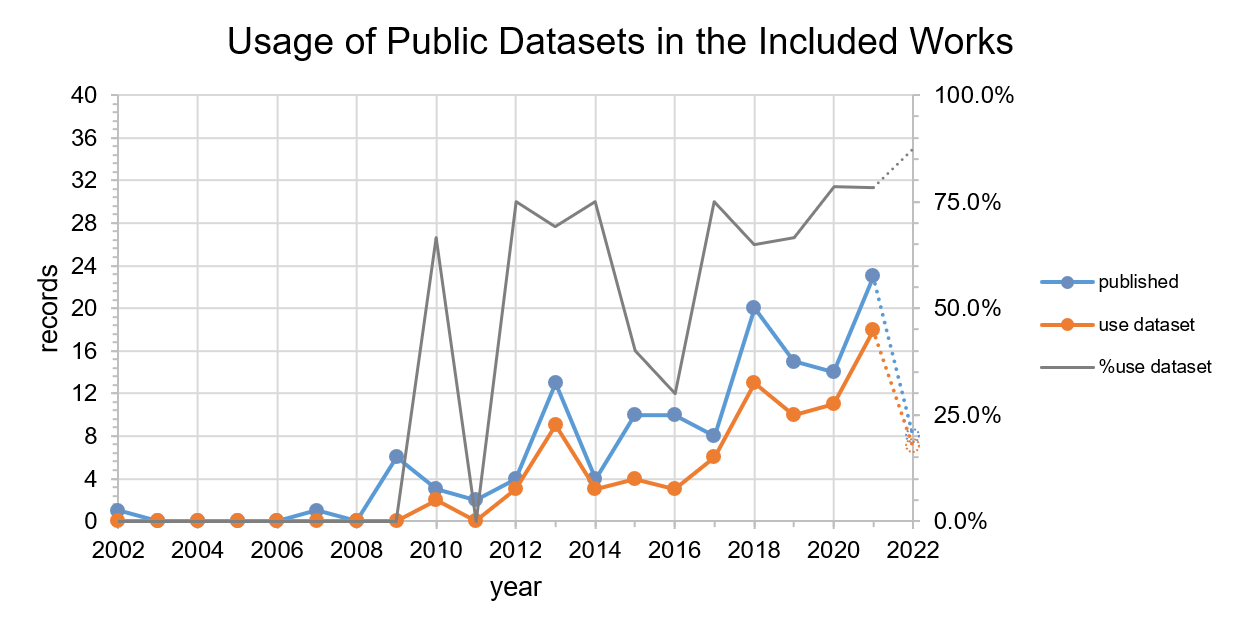
\includegraphics[width=\columnwidth]{figures/datasets.png}
  \caption{Evolution of the usage of public datasets per year considering the 142 included records in this review.}
  \label{fig:discussion:datasets}
\end{figure}

Although DE11 indicates which datasets are used in the experiments, this item does not characterize the datasets. Thus, Table~\ref{tab:discussion:datasets} presents a comparison table with the following items: long-term characteristics of the dataset in terms of the environment conditions (lighting, day and night sequences, weather and seasonal changing conditions, dynamic elements, and sparsity), type of environment (indoor, outdoor, or both), the domain of the agent used for acquiring data (ground, air, or water, and the commercial unit used if indicated), sensorization, if the dataset provides intrinsic and extrinsic calibration of the sensor setup used, type of ground-truth data, format, and long-term characteristics in terms of distance, time, and the number of runs. Next, the discussion focuses on comparing the datasets based on the column items presented in Table~\ref{tab:discussion:datasets} and correlating their usage in terms of DE1.

\onecolumn

\renewcommand{\arraystretch}{1.125}
\setlength{\tabcolsep}{1.5pt}

\begin{tiny}

\begin{longtable}{@{\extracolsep{1pt}}
p{0.065\textwidth}                          % Dataset name
c|                                          % Year
cccccc|                                     % Long-term
p{0.095\textwidth}                          % Environment
p{0.095\textwidth}|                         % Domain
c|                                          % Sensory setup: odo
ccccccc|                                    %                camera
cc|                                         %                laser
cccc|                                       %                radar, sonar, imu, gps
cc|                                         % Sensor calibrations
p{0.095\textwidth}p{0.095\textwidth}|       % Ground-truth + Format
ccccc@{}}                                   % Distance, time, \#sequences
  \caption{Datasets used in the 144 included records for long-term localization and / or mapping experiments. Legend: odo -- odometry (wheeled, laser, visual, inertial, or a combination of odometry sources, dist. -- total distance length of the dataset, path -- total path distance if repeated several times, time -- total operation time, int. -- time interval between the start and end acquisition dates / time instants (d/w/m/y equivalent to day/week/month/year, 0 if only 1 run), and seq. -- number of sequences of the dataset.}
  %\vspace{0.5em}
  \label{tab:discussion:datasets}\\

%% FIRST TABLE HEADER
\hline
&&
\multicolumn{6}{c|}{\textbf{Long-term}} &
&&
\multicolumn{14}{c|}{\textbf{Sensor}} &
\multicolumn{2}{c|}{\textbf{Calib.}} &
&&
&&&&\\
&&&&&&&&&&
\multicolumn{1}{c}{} &
\multicolumn{7}{c}{\textbf{camera}} &
\multicolumn{2}{c}{\textbf{laser}}  &
&&&&
&&
&&
&&&&\\
\cline{12-18}
\cline{19-20}
\textbf{Dataset} & \textbf{Year} &
\rotatebox{90}{\textbf{lighting}} & \rotatebox{90}{\textbf{day/night}} & \rotatebox{90}{\textbf{weather}} & \rotatebox{90}{\textbf{seasonal}} & \rotatebox{90}{\textbf{dynamics}} & \rotatebox{90}{\textbf{sparsity}} & 
\textbf{Environ.} & \textbf{Domain} & 
\multicolumn{1}{c}{\rotatebox{90}{\textbf{odo}}} &
\rotatebox{90}{\textbf{gray}} & \rotatebox{90}{\textbf{color}} & \rotatebox{90}{\textbf{monocular}} & \rotatebox{90}{\textbf{stereo}} & \rotatebox{90}{\textbf{omni}} & \rotatebox{90}{\textbf{RGBD}} & \multicolumn{1}{c}{\rotatebox{90}{\textbf{thermal}}} &
\rotatebox{90}{\textbf{2D}} & \multicolumn{1}{c}{\rotatebox{90}{\textbf{3D}}} &
\rotatebox{90}{\textbf{radar}} & \rotatebox{90}{\textbf{sonar}} & \rotatebox{90}{\textbf{IMU}} & \rotatebox{90}{\textbf{GPS}} &
\rotatebox{90}{\textbf{intrinsic}} & \rotatebox{90}{\textbf{extrinsic}} & 
\textbf{GT data} & \textbf{Format} & 
\rotatebox{90}{\textbf{dist.} (km)} & \rotatebox{90}{\textbf{path} (km)} & \rotatebox{90}{\textbf{time} (h)} & \rotatebox{90}{\textbf{int.} (d/w/m/y)} & \rotatebox{90}{\textbf{\#seq.}}\\
\hline
\endfirsthead

%% TABLE HEADER IN THE FOLLOWING PAGES
\multicolumn{27}{l}{\itshape{\tablename\ \thetable{}: continued from previous page}}
\vspace{0.5em}\\
\hline
&&
\multicolumn{6}{c|}{\textbf{Long-term}} &
&&
\multicolumn{14}{c|}{\textbf{Sensor}} &
\multicolumn{2}{c|}{\textbf{Calib.}} &
&&
&&&&\\
&&&&&&&&&&
\multicolumn{1}{c}{} &
\multicolumn{7}{c}{\textbf{camera}} &
\multicolumn{2}{c}{\textbf{laser}}  &
&&&&
&&
&&
&&&&\\
\cline{12-18}
\cline{19-20}
\textbf{Dataset} & \textbf{Year} &
\rotatebox{90}{\textbf{lighting}} & \rotatebox{90}{\textbf{day/night}} & \rotatebox{90}{\textbf{weather}} & \rotatebox{90}{\textbf{seasonal}} & \rotatebox{90}{\textbf{dynamics}} & \rotatebox{90}{\textbf{sparsity}} & 
\textbf{Environ.} & \textbf{Domain} & 
\multicolumn{1}{c}{\rotatebox{90}{\textbf{odo}}} &
\rotatebox{90}{\textbf{gray}} & \rotatebox{90}{\textbf{color}} & \rotatebox{90}{\textbf{monocular}} & \rotatebox{90}{\textbf{stereo}} & \rotatebox{90}{\textbf{omni}} & \rotatebox{90}{\textbf{RGBD}} & \multicolumn{1}{c}{\rotatebox{90}{\textbf{thermal}}} &
\rotatebox{90}{\textbf{2D}} & \multicolumn{1}{c}{\rotatebox{90}{\textbf{3D}}} &
\rotatebox{90}{\textbf{radar}} & \rotatebox{90}{\textbf{sonar}} & \rotatebox{90}{\textbf{IMU}} & \rotatebox{90}{\textbf{GPS}} &
\rotatebox{90}{\textbf{intrinsic}} & \rotatebox{90}{\textbf{extrinsic}} & 
\textbf{GT data} & \textbf{Format} & 
\rotatebox{90}{\textbf{dist.} (km)} & \rotatebox{90}{\textbf{path} (km)} & \rotatebox{90}{\textbf{time} (h)} & \rotatebox{90}{\textbf{int.} (d/w/m/y)} & \rotatebox{90}{\textbf{\#seq.}}\\
\hline
\endhead

%% TABLE FOOTER
\hline
\endfoot
\hline
\endlastfoot



\citetitle{dataset:fhw} & 2001 &  &  &  &  &  & x & indoor (museum) & ground (TOURBOT) & x &  &  &  &  &  &  &  & x &  &  &  &  &  &  &  & -- & CARMEN & -- & -- & 1.98 & -- & 1\\
\hline
\citetitle{dataset:fr079} & 2003 &  &  &  &  &  & x & indoor (office) & ground (robot) & x &  &  &  &  &  &  &  & x &  &  &  &  &  &  &  & -- & CARMEN & -- & -- & 0.29 & -- & 1\\
\hline
\citetitle{dataset:fr101} & 2003 &  &  &  &  &  & x & indoor (office) & ground (robot) & x &  &  &  &  &  &  &  & x &  &  &  &  &  &  &  & -- & CARMEN & -- & -- & 0.29 & -- & 1\\
\hline
\citetitle{dataset:intel03} & 2003 &  &  &  &  &  & x & indoor (office) & ground (robot) & x &  &  &  &  &  &  &  & x &  &  &  &  &  &  &  & -- & CARMEN & 0.506 & -- & 0.75 & -- & 1\\
\hline
\citetitle{dataset:mit-kilian} & 2004 &  &  &  &  &  & x & indoor (office) & ground (robot) & x &  &  &  &  &  &  &  & x &  &  & x &  &  &  &  & -- & CARMEN & 2.2 & -- & 2.5 & -- & 1\\
\hline
\citetitle{dataset:city-center-fabmap} & 2008 & x &  &  &  & x &  & outdoor (urban) & ground (robot) &  &  & x & x &  &  &  &  &  &  &  &  &  & x & x &  & GPS, manual & plain text (non-image), jpg (image) & 2 & -- & -- & -- & 1\\
\hline
\citetitle{dataset:lip6indoor} & 2008 &  &  &  &  &  &  & indoor (office) & ground (handheld) &  &  & x & x &  &  &  &  &  &  &  &  &  &  & x &  & manual & ppm (images) & -- & -- & 0.11 & -- & 1\\
\hline
\citetitle{dataset:lip6outdoor} & 2008 & x &  &  &  & x &  & outdoor (campus) & ground (handheld) &  &  & x & x &  &  &  &  &  &  &  &  &  &  & x &  & manual & ppm (images) & -- & -- & 0.3 & -- & 1\\
\hline
\citetitle{dataset:new-college-fabmap} & 2008 & x &  &  &  & x &  & outdoor (campus) & ground (robot) &  &  & x & x &  &  &  &  &  &  &  &  &  & x & x &  & GPS, manual & plain text (non-image), jpg (image) & 1.9 & -- & -- & -- & 1\\
\hline
\citetitle{dataset:stlucia07} & 2008 & x &  &  &  & x &  & outdoor (urban) & ground (car) &  & x &  & x &  &  &  &  &  &  &  &  &  &  &  &  & -- & -- & 66 & -- & 1.67 & -- & 1\\
\hline
\citetitle{dataset:bicocca-indoor} & 2009 & x &  &  &  & x & x & indoor (office) & ground (Robocom) & x & x & x & x & x & x &  &  & x &  &  & x & x &  & x & x & map model, laser-based & plain text (non-image), png (image) & -- & -- & 2.5 & 3d & 5\\
\hline
\citetitle{dataset:cold} & 2009 & x & x & x &  & x &  & indoor (office) & ground (Pioneer 3, ATRV Mini, PeopleBot) & x &  & x & x &  & x &  &  & x &  &  &  &  &  &  &  & laser-based, manual & plain text (non-image), jpg (image) & 0.92 & -- & 0.99 & -- & 76\\
\hline
\citetitle{dataset:malaga-2009} & 2009 & x &  &  &  & x &  & outdoor (parking, campus) & ground (car) &  &  & x & x &  &  &  &  & x &  &  &  & x & x & x & x & RTK-GPS & Rawlog MRPT & 6.358 & -- & -- & -- & 6\\
\hline
\citetitle{dataset:newcollege} & 2009 & x &  &  &  & x &  & outdoor (campus) & ground (Segway) & x & x & x &  & x & x &  &  & x &  &  &  & x & x & x & x & GPS & plain text (non-image), png (stereo), jpg (omni) & 2.2 & -- & 0.73 & -- & 1\\
\hline
\citetitle{dataset:albert-b} & 2010 & x &  &  &  &  & x & indoor (office) & ground (iRobot B21r) & x &  & x & x &  &  &  &  & x &  &  &  &  &  &  &  & -- & CARMEN (non-image), jpg (image) & -- & -- & 0.18 & -- & 1\\
\hline
\citetitle{dataset:cmu-vl} & 2011 & x &  &  & x & x &  & outdoor (urban) & ground (car) &  &  & x & x &  &  &  &  &  &  &  &  &  & x & x & x & GPS & -- & -- & 8.5 & -- & 1y & 16\\
\hline
\citetitle{dataset:ford} & 2011 & x &  &  &  & x &  & outdoor (campus, urban) & ground (car) &  &  & x &  &  & x &  &  & x & x &  &  & x & x & x & x & RTK-GPS & LCM log & -- & -- & -- & 2m & --\\
\hline
\citetitle{dataset:utias} & 2011 & x &  &  &  &  &  & indoor (empty space) & ground (iRobot Create) & x &  & x & x &  &  &  &  &  &  &  &  &  &  & x &  & external tracking system & jpg (image), dat (non-image) & -- & -- & 4.78 & -- & 9\\
\hline
\citetitle{dataset:alderley} & 2012 & x &  & x &  & x &  & outdoor (urban) & ground (car) &  &  & x & x &  &  &  &  &  &  &  &  &  &  &  &  & manual & -- & 16 & 8 & -- & -- & 2\\
\hline
\citetitle{dataset:tum-rgbd} & 2012 & x &  &  &  & x &  & indoor (office, industrial hall) & ground (handheld, Pioneer 3) &  &  & x &  &  &  & x &  &  &  &  &  & x &  & x & x & external tracking system & plain text (non-image), png (image + depth), ROS bag & 0.285 & -- & 0.35 & -- & 15\\
\hline
\citetitle{dataset:cobot} & 2013 & x &  &  & x & x & x & indoor (office) & ground (robot) & x &  & x &  &  &  & x &  & x &  &  &  &  &  &  & x & -- & ROS bag & 131 & -- & 260 & 2y3m & 1082\\
\hline
\citetitle{dataset:kitti} & 2013 & x &  &  &  & x &  & outdoor (urban) & ground (car) &  & x & x & x & x &  &  &  &  & x &  &  & x & x & x & x & RTK-GPS & png (image), binary (laser), plain text (imu, gps) & -- & -- & 1.18 & 8d & 61\\
\hline
\citetitle{dataset:mit-stata} & 2013 & x &  &  & x & x & x & indoor (office) & ground (PR2) & x &  & x &  & x &  & x &  & x &  &  &  & x &  &  & x & map model & ROS bag & 42 & -- & 38 & 1y9m & 84\\
\hline
\citetitle{dataset:nordlandsbanen} & 2013 & x &  & x & x &  &  & outdoor (railway) & ground (train) &  &  & x & x &  &  &  &  &  &  &  &  &  & x &  &  & GPS & mp4 (video stream), plain text (gps) & 2916 & 729 & 39.74 & -- & 4\\
\hline
\citetitle{dataset:gardens-qut} & 2014 & x & x &  &  & x &  & indoor, outdoor (campus) & ground (handheld) &  &  & x & x &  &  &  &  &  &  &  &  &  &  &  &  & ground-plane position & png (images), plain text (ground plane) & -- & -- & -- & -- & 3\\
\hline
\citetitle{dataset:lcas-strands} & 2014 & x & x &  & x & x &  & indoor (office) & ground (SCITOS-G5) &  &  & x &  &  &  & x &  & x &  &  &  &  &  &  & x & -- & ROS bag & -- & -- & -- & 1y1m & 368\\
\hline
\citetitle{dataset:kaist} & 2015 & x & x &  &  & x &  & outdoor (urban) & ground (car) &  &  & x &  & x &  &  & x &  &  &  &  & x & x & x & x & RTK-GPS & png (images), plain text (imu, gps) & 84 & -- & -- & 18d & 36\\
\hline
\citetitle{dataset:euroc} & 2016 & x &  &  &  &  &  & indoor (industrial hall, office) & air (AscTec Firefly) &  & x &  & x & x &  &  &  &  &  &  &  & x &  & x & x & external tracking system & ROS bag & 0.8936 & -- & 0.37 & -- & 11\\
\hline
\citetitle{dataset:nclt} & 2016 & x &  & x & x & x &  & indoor, outdoor (campus) & ground (Segway) &  &  & x &  &  & x &  &  & x & x &  &  & x & x & x & x & RTK-GPS, SLAM-based & binary (laser), tiff (image), plain text (non-laser or image) & 147.4 & -- & 34.9 & 1y4m & 27\\
\hline
\citetitle{dataset:kudamm} & 2017 & x &  &  &  & x &  & outdoor (urban) & ground (car) &  &  & x & x &  &  &  &  &  &  &  &  &  &  &  &  & manual & jpg (image) & -- & -- & -- & -- & 2\\
\hline
\citetitle{dataset:oxford-robotcar} & 2017 & x & x & x & x & x &  & outdoor (urban) & ground (car) & x &  & x & x & x &  &  &  & x & x &  &  & x & x & x & x & RTK-GPS & png (image), binary (laser), plain text (imu, gps, odo) & 1010.46 & 10 & -- & 1y8m & 133\\
\hline
\citetitle{dataset:yq21} & 2017 & x &  &  &  & x &  & outdoor (campus) & ground (car) &  &  & x & x & x &  &  &  &  & x &  &  & x & x & x & x & RTK-GPS & binary (laser), jpg (images), plain text (gps) & 23 & -- & 6.5 & 1w & 21\\
\hline
\citetitle{dataset:cmu-seasons} & 2018 & x &  &  & x & x &  & outdoor (urban) & ground (car) &  &  & x & x &  &  &  &  &  &  &  &  &  &  & x & x & manual & jpg (image) & -- & 8.5 & -- & 330d & 17\\
\hline
\citetitle{dataset:fas} & 2018 & x &  &  & x & x &  & outdoor (urban) & ground (car) &  &  & x &  & x &  &  &  &  &  &  &  &  & x &  &  & GPS, manual & jpg (image) & 110 & -- & -- & 3y & 3\\
\hline
\citetitle{dataset:robotcar-seasons} & 2018 & x &  & x &  & x &  & outdoor (urban) & ground (car) &  &  & x & x & x &  &  &  &  &  &  &  &  &  & x & x & manual & jpg (image) & -- & 10 & -- & 178d & 10\\
\hline
\citetitle{dataset:bonn} & 2019 &  &  &  &  & x &  & indoor (office) & ground &  &  & x &  &  &  & x &  &  &  &  &  &  &  & x & x & external tracking system & png (images, depth), plain text (imu, gps) & -- & -- & -- & -- & 26\\
\hline
\citetitle{dataset:cbd} & 2019 & x &  &  &  & x &  & outdoor (urban) & ground &  &  & x & x & x &  &  &  &  &  &  &  &  &  &  &  & manual & png (images) & -- & -- & -- & -- & 1\\
\hline
\citetitle{dataset:mulran} & 2020 &  &  &  &  & x &  & outdoor (urban) & ground (car) &  &  &  &  &  &  &  &  &  & x & x &  & x & x &  & x & SLAM-based & binary (laser), CSV (global pose, radar ray), png (radar polar image) & 41.2 & -- & -- & 2m15d & 12\\
\hline
\citetitle{dataset:robotcar-radar} & 2020 & x &  & x &  & x &  & outdoor (urban) & ground (car) & x &  & x & x & x &  &  &  &  & x & x &  & x & x & x & x & RTK-GPS, SLAM-based & png (image, raw laser, radar), binary (laser), plain text (imu, gps, odo) & 280 & 10 & -- & 1m & 32\\
\hline
\citetitle{dataset:usyd} & 2020 & x &  & x & x & x &  & outdoor (campus) & ground (car) & x &  & x & x &  &  &  &  &  & x &  &  & x & x & x & x & GPS & ROS bag & -- & -- & -- & 1y & 52\\
\hline
\citetitle{dataset:iplt} & 2021 & x & x & x & x & x &  & outdoor (parking) & ground (car) & x & x &  & x &  &  &  &  & x &  &  &  &  & x & x & x & GPS & ROS bag & -- & 0.2 & -- & 2y & 127\\
\hline
\citetitle{dataset:radiate} & 2021 & x & x & x &  & x &  & outdoor (parking, urban) & ground (car) &  &  & x & x & x &  &  &  &  & x & x &  & x & x & x & x & RTK-GPS & ROS bag & -- & -- & 4.98 & -- & --\\
\hline
\citetitle{dataset:ntu} & 2022 & x &  &  &  &  &  & indoor, outdoor (campus) & air (DJI M600) &  & x &  & x & x &  &  &  &  & x &  &  & x &  & x & x & external tracking system & ROS bag & 1.845 & -- & 0.9 & -- & 9\\



%  \end{tabular}}
%\end{table*}
\end{longtable}

\end{tiny}

\twocolumn

\renewcommand{\arraystretch}{1.25}
\setlength{\tabcolsep}{3pt}



\paragraph{Environment}

The outdoor environment is the most seen one in the 43 datasets, with 27 being acquired outdoors compared to 19 indoors, and 3 datasets (\citetitle{dataset:gardens-qut}, \citetitle{dataset:nclt}, and \citetitle{dataset:ntu}) having indoor and outdoor sequences.
The environment changing conditions more present in indoor datasets are lighting changes and dynamic elements, e.g., in office environments where the exterior and artificial light influence the visual perception and moving people increase environment dynamics (not only the people, but moving objects taken by persons).
Although night periods, weather and seasonal changes also influence indoor conditions, this influence is mostly in the lighting conditions and only appear in 4 indoor-only datasets (\citetitle{dataset:cold}, \citetitle{dataset:cobot}, \citetitle{dataset:mit-stata}, and \citetitle{dataset:lcas-strands}), accordingly to the respective dataset descriptions.
Similarly, the outdoor datasets are more affected by changing lighting and moving objects. However, these datasets consider more frequently and are more influenced by other changes. This influence is not only in lighting conditions but also in visual perception (color of the leaves in different seasons) and moving elements in the scene (water of the rain or moving tree branches due to strong wind).
In terms of recency, in the past 5 years, only 2 of the 14 datasets released during that period are in indoor locations. This recent tendency and the fact of 27/43 datasets having outdoor sequences indicate more interest in this type of environment by the included works in this review.

As for the diversity of the acquisition conditions, the most diverse datasets are \citetitle{dataset:cold}, \citetitle{dataset:lcas-strands}, \citetitle{dataset:nclt}, \citetitle{dataset:usyd}, \citetitle{dataset:radiate}, \citetitle{dataset:iplt}, and \citetitle{dataset:oxford-robotcar}. The latter two have all changing conditions in the environment, i.e., lighting, day/night sequences, dynamic elements, and weather and seasonal changes. Even though the remaining diverse datasets do not consider one of these conditions, the datasets are still interesting in the long-term localization and mapping context with a high diversity of environment conditions.

The datasets categorized as sparsity are intended for testing map maintenance algorithms to constrain the graph size in the graph SLAM formulation to the operation area and not to the trajectory length due to usually being available the full graph map of the dataset. Although these datasets are useful for evaluating map maintenance, they normally lack several other changing conditions that influence long-term localization and mapping while also all of those datasets being indoors. Only \citetitle{dataset:cobot} and \citetitle{dataset:mit-stata} datasets seem to be more diverse in terms of environment conditions by capturing sequences with different lighting conditions and dynamic elements in the scene.


\paragraph{Sensorization}

In terms of the type of sensors used for acquiring data, the ones utilized in the datasets are odometry (wheeled, visual, inertial, laser, or a combination of different odometric sources), cameras (monocular, stereo, omnidirectional, RGBD, or thermal), lasers (2D/3D), radar, sonar, IMU, and GPS, similar to the sensors found in the data extraction phase of this review. The more common type of sensor is camera used in 37/43 (86\%) datasets. This predominance is conformal with the high usage in 104/142 (73.2\%) included works and occurrence of related keywords in the analysis presented in Figure~\ref{fig:overview:kw} (both vision and camera keywords appear in the graph with 18 and 7 occurrences, respectively), indicating an interest of using camera sensors in data acquisition and long-term localization and mapping.
Also, the omnidirectional vision used in 5 datasets can be accomplished by using an hyperbolic mirror (\citetitle{dataset:bicocca-indoor}, \citetitle{dataset:cold}), joining the image of several cameras and using their extrinsic calibrated parameters, or using an omnidirectional camera (\citetitle{dataset:ford}, \citetitle{dataset:nclt}, \citetitle{dataset:newcollege}) such as the Point Grey LadyBug 2 5-view.
Although the thermal camera is only present in \citetitle{dataset:kaist}, this sensor can be interesting for building inspection \parencite{yue-et-al:2020:9197072}.

Moreover, datasets used in the included works recently released also use 3D laser (or LiDAR) and radar sensors. Although the older dataset with 3D laser is from 2011 (\citetitle{dataset:ford}), 5/10 (50\%) datasets using this sensor were released over the past 5 years from a total of 14 datasets released in this same period. This trend is noted also when analyzing the DE7 item of the included works, where 24/27 (89\%) methods using a 3D laser were proposed since 2018, indicating a recent importance of this sensor for long-term localization and mapping.
As for radar data, all 3 datasets using the sensor (\citetitle{dataset:mulran}, \citetitle{dataset:robotcar-radar}, and \citetitle{dataset:radiate}) were released since 2020. A corresponding recency is noted in included works with 3/4 (75\%) methods (\cite{martini-et-al:2020:s20216002}, \cite{yin-et-al:2021:661199}, and \cite{hong-et-al:2022:02783649221080483}) using the sensor are also from 2020 onwards. This recent usage indicates a recent interest of using radar data within the scope of this review's topic, probably due to being less affected by changing lighting or weather conditions compared to visual sensors~\parencite{hong-et-al:2022:02783649221080483}.

As for the other sensors used in the dataset, odometry data, IMU, 2D laser, and GPS are also extensively used in the datasets.
The first two provide relative motion information of the vehicle and are used in 16 and 17 datasets and 33 and 19 included works, respectively.
Although the 2D laser is used in 17 datasets, 15 of those are from 2016 and previous years. However, the sensor is still used in the included works over the years, especially in indoor environments, with 21/25 works for indoors using 2D lasers.
As for GPS data, this sensor is usually used as ground-truth data, as will be discussed later.

Sensor calibration is important for achieving long-term localization and mapping, not only for avoiding the propagation of inconsistency pose errors between sensors through time, but also to process the perceived data from the environment in the same coordinate referential frame. The intrinsic calibration is usually relative to camera sensors, where 25/37 (68\%) datasets with this sensor provide the intrinsic parameters to the user. Some of the datasets with cameras do not provide those parameters due to being intended only for image-based place recognition (e.g., \citetitle{dataset:city-center-fabmap}, \citetitle{dataset:cbd}, or \citetitle{dataset:fas}).
In terms of extrinsic calibration, 24/43 (56\%) datasets provide these parameters, being useful for evaluating methods where the parameters are required to be processed in the same reference frame.

The datasets more diverse in terms of their sensor setup are \citetitle{dataset:bicocca-indoor}, \citetitle{dataset:oxford-robotcar}, and \citetitle{dataset:robotcar-radar}, with 7, 6, and 6 different types of sensors, respectively.


\paragraph{File format}

Most of the datasets used by the included works define a specific format for organizing the respective data. These formats use standard file types such as plain text, CSV, or binary files having the advantage of not being tied to any particular software. Even so, there are common characteristics between those specific formats.
Images are usually saved in JPG or PNG files, whereas PNG files are also used in the datasets for saving depth information of RGBD sensors.
The laser data is usually saved in binary files due to its easiness for parsing by different programming languages and size considerations~\parencite{dataset:kitti,dataset:oxford-robotcar}.
Another common aspect of specific formats found in the datasets of Table~\ref{tab:discussion:datasets} is the use of plain text or CSV files to save IMU, GPS, and/or odometry data.
As for radar data, the respective polar representations are saved in PNG files.

However, the datasets also make available standard log formats compatible with different types of sensor data.
The most used one is ROSbag from the Robot Operating System (ROS) framework in 9 datasets. This log format is compatible with common messages defined in ROS for different sensors\footnote{\url{http://wiki.ros.org/common_msgs}}.
The other standard format used in more than one dataset is CARMEN log files defined in the CARMEN robot navigation toolkit\footnote{\url{https://carmen.sourceforge.net/}}. Although this log format supports different sensor data such as odometry or lasers, the CARMEN navigation toolkit is not updated since 2008 (version 0.7.4-beta), considered to be deprecated.


\paragraph{Usage relation with the included records}

As for relating the datasets usage with this review's included works, the datasets can be related with the DE1 categorization of the records. From the appearance category in DE1, 50/75 (67\%) works use 32 different public datasets from Tabl~\ref{tab:discussion:datasets} to evaluate the proposed methodologies. The datasets most used are \citetitle{dataset:kitti}, \citetitle{dataset:nordlandsbanen}, \citetitle{dataset:nclt}, \citetitle{dataset:stlucia07}, and \citetitle{dataset:oxford-robotcar} (13, 11, 9, 8, and 8 usages). \citetitle{dataset:kitti} is also the most used overall, given the 26 works utilizing it for evaluation. However, this dataset and \citetitle{dataset:stlucia07} do not have seasonal nor weather changing conditions that greatly influence the appearance invariance of the methods, as discussed in Section~\ref{sec:discussion:appearance}, even though those datasets have high usage by the appearance-related works. Indeed, more recent datasets such as \citetitle{dataset:nclt} or \citetitle{dataset:oxford-robotcar} already widely used for evaluation, or also \citetitle{dataset:usyd} and \citetitle{dataset:radiate} would be suitable for evaluating the appearance invariance of the localization and mapping algorithms due to the datasets' diversity in terms of varying conditions.

Although the works categorized as dynamics and sparsity also use public datasets for evaluation, the usage is slightly lower than for appearance-related methods (44\% and 51\%, respectively, compared to 67\%).
\citetitle{dataset:kitti}, \citetitle{dataset:tum-rgbd}, and \citetitle{dataset:lcas-strands} are the only datasets used in more than one work categorized as dynamic (7, 6, and 2 usages, respectively), considering a total of 10 different datasets used by these works. However, \citetitle{dataset:kitti} and \citetitle{dataset:tum-rgbd} could be not the most suitable datasets for evaluating the performance over different levels of dynamics in the environment due to the smaller total operation time of 1.18h and 0.35h, respectively, compared to other datasets classified as having dynamic elements in Table~\ref{tab:discussion:datasets}. For example, \citetitle{dataset:lcas-strands} has a time frame of 1 year and a month in an indoor office environment capturing different motion frequencies or habits of the persons working at the scene with an average of 1 daily acquisition run. \citetitle{dataset:oxford-robotcar} and \citetitle{dataset:usyd} are also interesting due to the long time frames of the data acquisition (1 year and 8 months, and 1 year, with 133 and 52 runs, respectively). Also, \citetitle{dataset:iplt} is captured in a parking lot environment capturing semi-static and dynamic moving cars in the scene.
As for sparsity-related works, 22 different datasets are used in the experiments, whereas \citetitle{dataset:kitti}, \citetitle{dataset:intel03}, \citetitle{dataset:mit-kilian}, \citetitle{dataset:mit-stata}, and \citetitle{dataset:euroc} being the most utilized ones (6, 5, 3, 3, and 3 usages, respectively). \citetitle{dataset:kitti} and \citetitle{dataset:euroc} are used for evaluating feature management techniques, though these datasets have small operation time frames and, possibly, trajectory lengths. Although \citetitle{dataset:mit-stata} would seem like a good dataset for evaluating the sparsity due to the long trajectory length and time frame (42km and 38h, respectively), the dataset's description indicates that hardware and calibration problems in the data acquisition setup may have created inconsistencies in the data. As for \citetitle{dataset:intel03}, \citetitle{dataset:mit-kilian}, and other datasets classified as sparsity in Table~\ref{tab:discussion:datasets}, these are widely used for graph sparsification due to repeated passages in same locations with a total of 15 usages, even though those datasets have usually only 1 data sequence. Other recent datasets could also be interesting for evaluation sparsification techniques of the map such as \citetitle{dataset:oxford-robotcar} and \citetitle{dataset:mulran}, given the repeated passages over the 10km path and the long trajectory length of 41.2km, respectively.

Furthermore, 5/7 multi-session works used datasets, whereas the \citetitle{dataset:mit-stata} and \citetitle{dataset:intel03} being the most used ones with 2 usages each. While each data sequence of \citetitle{dataset:mit-stata} may represent a single session~\parencite{lázaro-et-al:2018:8594310}, the unique data sequence of \citetitle{dataset:intel03} can be split into different sessions~\cite{latif-et-al:2012:6385879}. This approach is valid for applying to other datasets in Table~\ref{tab:discussion:datasets}.
As for the computational categorization on DE1, this category does not relate to the datasets used in the experiments because the computational efficiency is more dependent on the proposed localization and/or mapping algorithm than on the data.

In terms of multi-robot works~\parencite{gadd-newman:2016:7759843,zhang-et-al:2018:1729881418780178,karaoguz-bozma:2020:2,yue-et-al:2020:9197072} identified by the DE4, even though the dataset \citetitle{dataset:utias} collects data from 5 robots and being the only multi-robot dataset in Table~\ref{tab:discussion:datasets}, it is only used in \cite{nobre-et-al:2018:8461111} to test the reconfiguration of landmarks in the scene in different runs for single-robot localization and mapping. The only datasets used in multi-robot works are \citetitle{dataset:kitti} in \cite{zhang-et-al:2018:1729881418780178} and \citetitle{dataset:cold} in \cite{karaoguz-bozma:2020:2}. These works assume that different data sequences are acquired by different agents or segment the sequence in data subsets, similar to the evaluation with datasets of multi-session works.
However, the fact that only 4 multi-robot works are included in this review and only 1 public dataset used in the included records is acquired with multiple vehicles could indicate that the use of multi-robot systems is not yet widely studied in the long-term localization and mapping topic.



\subsubsection{Distance and time considerations}

Next, analyzing the total trajectory length of the private experiments on the included records (DE10 on Table~\ref{tab:a2:data-extraction}) and public datasets (see Table~\ref{tab:discussion:datasets}), 5 works and 6 datasets have a length greater than 100km.
Higher values on the trajectory length indicate possibly more interesting data for evaluating sparsity management techniques discussed in Section~\ref{sec:discussion:sparsity}, given that the desired behavior of a mapping algorithm is its scalability being only dependent on the environment size and not on the trajectory length. Although the total trajectory length does not necessarily relates directly with the environment area, the latter is rarely seen in the experiments description, and even for the trajectory length, only 36/77 works that perform private experiments and 22/43 datasets indicate the length.

The other distance measure considered in this review to characterize the experimental data is the one relative to repeating the same path, with 7/8 datasets and 3/8 included works that specify this metric having a repetitive path distance greater than 8km and more than 1 run. These low numbers do not necessarily indicate incomplete information in the experimental description due to a data acquisition can be performed on non-repetitive routes. Even so, repeating the same exact path under different environment conditions (i.e., appearance variance) could be a case study for evaluating the appearance invariance of localization and mapping algorithms discussed in Section~\ref{sec:discussion:appearance}.

In terms of time-related long-term characteristics of experimental data, longer total operation times indicate a robust evaluation of the proposed localization and mapping algorithms over long continuous periods, and greater time interval suggests data acquired under severe changing conditions (not only in the environment appearance but also semi-static modifications in the scene). However, only 2/10 works performing private experiments and indicating the total operation time test their methods over a total of 8h (equivalent to a work day), while also only 4/23 datasets that define the total log time in their description have more than 8h of data. On the contrary, 41/77 works and 18/43 datasets characterize the interval between the first and the last data sequence, which of those 29 works performing private experiments and 17 datasets have at least a 1 week interval. These results indicate that even though the included works in this review use experimental data with greater time intervals, often several days or weeks, not so much importance is given towards the total operation time.



\subsubsection{Ground-truth data}

As for the types of ground-truth data found in the included works (see DE9 in Table~\ref{tab:a2:data-extraction}) and the public datasets used for evaluation (see Table~\ref{tab:discussion:datasets}), the manual annotation is one of the most used types of ground-truth including image to image association (e.g., useful for evaluating image-based place recognition), manual alignment of maps~\parencite{biswas-veloso:2013:0278364913503892}, or manually segmenting images~\parencite{dataset:kitti}.
Although GPS-based data is also widely used in the experiments, whereas the RTK-GPS variant improves the pose precision compared to the basic positioning system, GPS is meant for use in outdoor environments. The alternative for indoor environments used in the experiments is external tracking systems using, e.g., reflective markers put on the robot to track them through systems such as OptiTrack\footnote{\url{https://optitrack.com/}} or Vicon\footnote{\url{https://www.vicon.com/}} to provide precise measurements of the robot's pose.
Simulation data used in 10 included works can also provide precise ground-truth data for the robot's pose or other types of information, even though not in a real environment.

Moreover, SLAM or laser-based ground-truth data are also found in the experimental evaluation of the included works and public datasets. The experimental methodology uses localization and mapping algorithms other than the one being evaluated to provide ground-truth data usually using a different sensor setup, or using the same algorithm but including all data sessions or global optimization over the entire pose graph.
Specifically, laser-based localization is widely used in the included works as ground-truth data to evaluate vision-based methods~\parencite{nuske-et-al:2009:20306}.
Similarly to SLAM-based ground-truth data, the experimental results of localization and mapping methods without pruning are also used as a reference for evaluating sparsification algorithms~\parencite{carlevaris-bianco-et-al:2014:2347571}.

As for model-based ground-truth data, the work of \cite{boniardi-et-al:2019:003} and the datasets \citetitle{dataset:bicocca-indoor} and \citetitle{dataset:mit-stata} propose the use of floor plans as a model of the environment to align the current estimation with the model and obtain a ground-truth for the trajectory of the robot on the map.
\cite{ozog-et-al:2016:21582}  is the other method using map models in the experimental evaluation but in the context of ship hull inspection, where the current map estimation is aligned with the ship hull CAD model for obtaining the trajectory ground-truth data.
However, the use of map-based ground-truth data to evaluate the mapping process is not seen in the included works, other than performing a visual quality evaluation over the mapping results and the sensor data.





\subsection{Evaluation metrics}
\label{sec:discussion:metrics}

The final topic of discussion over the included works in this review is the analysis on evaluation metrics used for assessing the performance of the proposed methodologies (see DE12 in Table~\ref{tab:discussion:datasets}).
This analysis is organized by metrics intended for place recognition, evaluation of the robot pose, assessment of map sparsity, and computational performance.



\subsubsection{Place recognition}

The evaluation of place recognition performance within the context of this review is intrinsically related to the invariance to changing conditions of long-term localization and mapping, and so, works categorized as appearance in DE1. The most used metrics for place recognition in the included works are precision and recall, where 50/142 works use these metrics in the experimental evaluation, and from those works 39 are categorized as appearance. These metrics characterize the performance of recognizing successfully different places related to the number of true and false positives and true and false negatives, and also include the precision-recall curve where a greater area under the curve indicates a better classifier for place recognition.

Other metrics less used in the included works but also important are the confusion matrix, the localization success rate, and the f-score and f-beta measures. The confusion matrix associates the predicted place to the true value in the case of each data entry representing a unique place, and a unique diagonal in the matrix would be the ideal result. This matrix is also used for comparing the data stream versus a reference database, where the appearance of multiple diagonals in the matrix indicates the capability of the place recognition algorithm to perform loop closure relative to the database.
The localization rate is the ratio between the number of successful localization versus and the attempts. As for the f-score and f-beta metrics, these measures combines the precision and recall in an unique value, where the f-beta allows the weighting of precision versus recall depending on which is more important for the method's use case.



\subsubsection{Robot pose}

Robot pose-related metrics are widely used in works categorized as appearance, dynamic, and sparsity methods (21/75, 18/32, and 16/45, respectively). The pose error indicates if the localization algorithm is affected by changing conditions over time. For dynamic-related methods, the pose error is also useful to show the influence of moving elements in the scene on the localization performance. As for sparsification techniques, the pose error cn characterize the influence of the map pruning algorithm over the localization estimator.

In terms of evaluating the robot pose, the pose error is also one of the most used metrics in the included works (50/142). These works evaluate the pose error metric in terms of its instant measurement over time or relative to a data sequence in terms of the mean, standard deviation, and/or RMSE values of the pose error. Also, a specific measure of pose error used in 15/142 works is the Absolute Trajectory Error (ATE) usually computed over an entire trajectory. This metric requires the time alignment between the localization estimation and the ground-truth data and computes the mean and standard deviation of the estimation differences between samples with the same time instant\footnote{See definition of ATE in the TUM dataset (\url{https://vision.in.tum.de/data/datasets/rgbd-dataset/tools\#absolute\_trajectory\_error\_ate}) and in the RAWSEEDS benchmarking toolkit (\url{http://www.rawseeds.org/rs/methods/view//9})}.

The covariance of the pose estimation is also considered in the included works for evaluating the robot pose error, where the covariance matrix represents the uncertainty of the robot's pose over an experiment. Also, in \cite{hochdorfer-schlegel:2009}, the covariance matrix's eigenvalues are used to evaluate the uncertainty of the estimator, where greater values represent greater uncertainties. Instead of computing the eigen values from the covariance matrix, \cite{dayoub-duckett:2008:4650701} computes these values from the inverse covariance matrix, and so, the logic also inverts relative to \cite{hochdorfer-schlegel:2009}, where smaller eigen values would mean smaller uncertainties in that case.



\subsubsection{Map sparsity}

As for evaluating the map sparsity, this evaluation is inherently related to the sparsity category of DE1.
In terms of metrics, the analysis of the evolution of the number of nodes is widely used in 19/45 sparsity-related works. This metric is useful to study the evolution of the graph size in the graph formulation of SLAM over the operation time and/or trajectory length.
The number of edges over time or the edge reduction ratio compared to no pruning data also indicate growth over time of the edges, while the gamma index of a graph (ratio between the number of existing edges and the possible ones) indicates the current sparsity over the graph connectivity.
Another important metric for evaluating the graph sparsification is the Kullback-Leibler Divergence (KLD) measure that defines the difference between two probabilistic distributions. The included works use the KLD to compare the information loss between the sparse graph and the one without pruning, in which a 0 value of KLD would mean that the two distributions have identical information, and so the graph pruning algorithm was able to remove only redundant data.
More generally, the evaluation of the number of map points over time is also presented in the results of sparsity-related works.



\subsubsection{Computational performance}

Finally, the evaluation of the computational performance is widely analyzed in the included works. This evaluation is not necessarily related to only the computational category of DE1 because an algorithm's computational performance impacts its online execution. Considering the 110 methods with online execution modes identified in Table 1 by DE5, 76 (69.1\%) works evaluate the computational resources required for online execution of the proposed methodology, indicating the importance of this type of experimental analysis in the included works. In terms of computational performance metrics, the execution time measurement is most used one being evaluated in 69 works. However, other metrics such as the runtime memory or the computational complexity are considered in the included works for evaluating the computational resources required to execute the proposed methodologies.





\section{Challenges and Future Directions}
\label{sec:future}

The growing interest in mobile robots and their usage in different applications and complex environments stress the importance of improving the robustness of autonomous systems. Although the localization and mapping algorithms included in this study help achieve long-term operations, these algorithms are not bulletproof.
So, in addition to the challenges discussed in Section~\ref{sec:discussion}, other potential challenges related to lifelong SLAM and research directions are listed below.



\paragraph{Vision-based global place recognition}

Given the limited field of view characteristic of vision sensors (apart from omnidirectional cameras), the analysis of the included records shows that it is still challenging to recognize places using vision-based global descriptors.
The limited field of view influences the visual content of the image, as shown in the experimental results of \cite{qin-et-al:2020:103561}, where the method significantly reduced its performance due to viewpoint variance.

One possible direction could be the usage of data augmentation as in \cite{tang-et-al:2021:17298814211037497} for learning global visual descriptors, even though the latter work does not clarify to what extent augmented data helped in viewpoint variance.
Another possible solution would be the use of omnidirectional vision, even though the networks traditionally used for learning CNN-based features (considered more discriminative compared to handcrafted features, as previously discussed in Section~\ref{sec:discussion:appearance:cnn}) may not be directly applicable due to the different aspect ratio of omnidirectional images.



\paragraph{Dynamics modeling}

Most of the included works modeling the environment dynamics determine the observations as static (permanent change), semi-static (short-term static object or static at the current observation instant), or dynamic (moving object in the scene) by either representing them in maps associated with different discrete meanings of dynamics or reasoning the relation between their semantic class and the expected dynamics. However, the determination of a dynamics value for the observations could be interesting to observe its evaluation over time for predicting the environment dynamics or accounting them in the localization and mapping processes.

In the included works, \cite{tipaldi-et-al:2013:0278364913502830} and \cite{rapp-et-al:2015:77} use Markov-based processes for predicting environment dynamics. However, these works assume the independence of observations, which could not be valid because static and dynamic objects may influence the dynamics of their surroundings. While FreMEn~\parencite{krajník-et-al:2017:2665664} estimates the dynamicity through spectral analysis, this method assumes only periodic changes in the environment. Even though ARMA~\parencite{wang-et-al:2020:9468884} models both aperiodic and periodic changes, its offline operation does not allow an online estimation of the observations' dynamicity value. So, it remains a challenge estimating online the dinamicity of environment observations unless the localization and mapping algorithms assume discrete levels for dynamics.



\paragraph{Online graph sparsification}

In the graph formulation for the SLAM problem, the methods GLC~\parencite{carlevaris-bianco-et-al:2014:2347571} and NFR~\parencite{mazuran-et-al:2016:0278364915581629} stand out in terms of their graph sparsification results, obtaining a graph growth approximately dependent only on the environment area and not on the operation time or trajectory length. However, these methods are mostly intended for offline execution (e.g., between operation sessions) due to their additional computational cost when operating online.
\cite{ila-et-al:2017:0278364917691110} seems to be an interesting alternative by proposing an incremental solution focused on the computational cost of graph sparsification. However, experimental results only showed that the method slows the graph's growth rate instead of bounding when operating in the same environment area. Even though \cite{boniardi-et-al:2019:003} achieves a bounded computation time by pruning nodes based on topological consistency, it remains to be seen the results of graph sparsification without the CAD prior and in more highly dynamic environments.
Thus, online graph sparsification is still an open research question and important for extended time periods of continuous operation periods.



\paragraph{Decentralized computation}

Given the computational complexity inherent to SLAM, an alternative to running locally in the robot is decentralizing the algorithm's execution, offloading some parts to external agents with more computational power.
In the included works, while \cite{ali-et-al:2020:3389033} implements a mobile-edge parallel execution bounding the computation time in the local device, the execution time and memory of the edge device grow over time. Furthermore, the state of the communication link influences the quality of localization and mapping, as shown in Ding when evaluating the proposed cloud-based visual localization system with different network delays and packet losses.
Although the solution proposed by \cite{ding-et-al:2019:8968550} can deal with delays up to 5s, the method requires a permanent link with the cloud due to the robot only performing localization.

Overall, the topic of decentralized computing either by using edge devices or cloud-based solutions is still not well studied in the context of long-term localization and mapping. For example, the external devices could be able to perform global optimizations and searches, improving the initial estimations given by the robot. Another use case for decentralized long-term SLAM would be the external agent keeping observations of the same location at different time instants to evaluate the appearance and dynamic changes in the scene, while the robot would access the most updated, invariant, and stable map for localization.



\paragraph{Multi-robot long-term SLAM}

Most of the current research discussed in this review focuses on single-robot long-term SLAM. Extending the current research for multi-robot systems would be interesting for optimizing the autonomous systems operation. However, the consideration of multi-robots also creates new challenges. One of would could be the decentralized and distribution SLAM execution within the multi-robot system (e.g., which information to exchange between robots) and the possibility of having external agents (e.g., edge or cloud devices) to the multi-robot system for offloading computation tasks. Another challenge would be considering the heterogeneous characteristics of the robots (domain, sensors, motion constraints) in merging information.



\paragraph{Active exploration}

Information-driven exploration is an interesting research topic consisting on actively planning the locations and times for the robot to visit. In the context of lifelong localization and mapping, active navigation could plan the robot trajectory, e.g., for avoiding locations that the robot predicts to be highly dynamic or for generating specific mapping tasks in locations known to be very susceptible to appearance changes to maintain an up to date representation of the environment.
One example found in the included works is \cite{santos-et-al:2016:2516594} that uses the dynamic prediction provided by the FreMEn module for the planner to predict which areas are more likely to change and define the locations to explore.
However, achieving active navigation would require a tightly coupling the planning process with the robot's localization and mapping estimations. Also, the reasoning and modeling of the environments changes would play an important role for planning the tasks.



\paragraph{Human-to-Machine Interfaces}

The persons interacting day-to-day with autonomous systems may also play an important role in achieving a successful long-term operation. An operator of the system can provide a priori information useful for the localization and mapping tasks. For example, if the relocalization estimation was not successful based on the current environment representation, the operator could define the robot's initial pose. Another example could be the dynamics modeling accounting also the operator input for specific areas.

However, the interaction with the user should not be through raw sensor data due to possibly increasing the need for special training for the operator, especially in industrial applications. \cite{boniardi-et-al:2019:003} presents an interesting work in terms of using CAD prior for localization and mapping while facilitating the interaction with the user. Another potential direction could be using higher levels of information for interaction such as high-level geometric and semantic features perceived by the robot.

\section{Limitations of the Study}
\label{sec:limitations}

Although this study follows a systematic methodology for selecting the included works in the review, the methodology followed by this study has limitations. One limitation is related to the goal of overview the long-term SLAM topic instead of providing an in-depth analysis, discussion, and comparison focused on a single challenge intrinsic to lifelong autonomy. This limitation leads to an extensive and complex discussion of the included works that may possibly not cover all the details of the proposed methods in the included records.
However, none of the existent reviews in SLAM focus on the long-term localization and mapping problem nor clarify the selection methodology of the works included in their studies. Also, not focusing on a single challenge related to long-term SLAM provides a broader and interesting discussion of the topic, given that some challenges may be related between each other. For example, removing elements from the current map estimation considered to be outdated due to appearance changes is related to both environment changing conditions and map management.
Even so, the broader discussion itself is a limitation of the study, and future ones may prefer to focus only on methodologies related to a single challenge of lifelong SLAM.

Furthermore, the quality assessment in the selection phase of this study only considers 2 criteria associated with the topic of this study, namely, QE3 and QE5. While the remaining quality criteria evaluate the eligible records in terms of their scientific contribution, only 2 out of 9 being related to the topic of the review may be considered a limitation of this study. This limitation is related to the previous one. Indeed, the QE not considering specific challenges and characteristics of long-term autonomy tries to avoid the a priori knowledge of the authors to the review on lifelong SLAM biasing the methods' selection methodology.
However, even though the followed methodology obtained two distinct peaks in the QE scores (see Figure~\ref{fig:methodology:qe}) that could be interpreted as belonging to 2 different clusters -- records to exclude versus the ones to include in the review --, the inclusion of more QE criteria would perhaps improve the distinction between the clusters.

The other limitation of this study is the discussion of the public datasets. Instead of considering a different query to find and select datasets, the discussion focused only on the ones used in the experiments by the included works. While this selection approach allowed the identification of 43 different datasets, it does not mean that these datasets are the best to use to evaluate methodologies related to long-term SLAM due to the identification of the datasets discussed in this study may be biased by the included works themselves. Although the main focus of this systematic literature review is on ways to achieve lifelong autonomy and not only on the experimental data, future studies should consider to review separately the datasets from the methodologies. Still, the inclusion of an analysis of common used datasets by the included works improves the interest of this review for researchers interested in long-term localization and mapping.

\section{Conclusions}
\label{sec:conclusions}



\end{document}
